\documentclass[]{book}
\usepackage{lmodern}
\usepackage{amssymb,amsmath}
\usepackage{ifxetex,ifluatex}
\usepackage{fixltx2e} % provides \textsubscript
\ifnum 0\ifxetex 1\fi\ifluatex 1\fi=0 % if pdftex
  \usepackage[T1]{fontenc}
  \usepackage[utf8]{inputenc}
\else % if luatex or xelatex
  \ifxetex
    \usepackage{mathspec}
  \else
    \usepackage{fontspec}
  \fi
  \defaultfontfeatures{Ligatures=TeX,Scale=MatchLowercase}
\fi
% use upquote if available, for straight quotes in verbatim environments
\IfFileExists{upquote.sty}{\usepackage{upquote}}{}
% use microtype if available
\IfFileExists{microtype.sty}{%
\usepackage{microtype}
\UseMicrotypeSet[protrusion]{basicmath} % disable protrusion for tt fonts
}{}
\usepackage[margin=1in]{geometry}
\usepackage{hyperref}
\hypersetup{unicode=true,
            pdftitle={Técnicas de Remuestreo},
            pdfauthor={Ricardo Cao Abad (rcao@udc.es) y Rubén Fernández Casal (ruben.fcasal@udc.es)},
            pdfborder={0 0 0},
            breaklinks=true}
\urlstyle{same}  % don't use monospace font for urls
\usepackage{natbib}
\bibliographystyle{apalike}
\usepackage{color}
\usepackage{fancyvrb}
\newcommand{\VerbBar}{|}
\newcommand{\VERB}{\Verb[commandchars=\\\{\}]}
\DefineVerbatimEnvironment{Highlighting}{Verbatim}{commandchars=\\\{\}}
% Add ',fontsize=\small' for more characters per line
\usepackage{framed}
\definecolor{shadecolor}{RGB}{248,248,248}
\newenvironment{Shaded}{\begin{snugshade}}{\end{snugshade}}
\newcommand{\KeywordTok}[1]{\textcolor[rgb]{0.13,0.29,0.53}{\textbf{#1}}}
\newcommand{\DataTypeTok}[1]{\textcolor[rgb]{0.13,0.29,0.53}{#1}}
\newcommand{\DecValTok}[1]{\textcolor[rgb]{0.00,0.00,0.81}{#1}}
\newcommand{\BaseNTok}[1]{\textcolor[rgb]{0.00,0.00,0.81}{#1}}
\newcommand{\FloatTok}[1]{\textcolor[rgb]{0.00,0.00,0.81}{#1}}
\newcommand{\ConstantTok}[1]{\textcolor[rgb]{0.00,0.00,0.00}{#1}}
\newcommand{\CharTok}[1]{\textcolor[rgb]{0.31,0.60,0.02}{#1}}
\newcommand{\SpecialCharTok}[1]{\textcolor[rgb]{0.00,0.00,0.00}{#1}}
\newcommand{\StringTok}[1]{\textcolor[rgb]{0.31,0.60,0.02}{#1}}
\newcommand{\VerbatimStringTok}[1]{\textcolor[rgb]{0.31,0.60,0.02}{#1}}
\newcommand{\SpecialStringTok}[1]{\textcolor[rgb]{0.31,0.60,0.02}{#1}}
\newcommand{\ImportTok}[1]{#1}
\newcommand{\CommentTok}[1]{\textcolor[rgb]{0.56,0.35,0.01}{\textit{#1}}}
\newcommand{\DocumentationTok}[1]{\textcolor[rgb]{0.56,0.35,0.01}{\textbf{\textit{#1}}}}
\newcommand{\AnnotationTok}[1]{\textcolor[rgb]{0.56,0.35,0.01}{\textbf{\textit{#1}}}}
\newcommand{\CommentVarTok}[1]{\textcolor[rgb]{0.56,0.35,0.01}{\textbf{\textit{#1}}}}
\newcommand{\OtherTok}[1]{\textcolor[rgb]{0.56,0.35,0.01}{#1}}
\newcommand{\FunctionTok}[1]{\textcolor[rgb]{0.00,0.00,0.00}{#1}}
\newcommand{\VariableTok}[1]{\textcolor[rgb]{0.00,0.00,0.00}{#1}}
\newcommand{\ControlFlowTok}[1]{\textcolor[rgb]{0.13,0.29,0.53}{\textbf{#1}}}
\newcommand{\OperatorTok}[1]{\textcolor[rgb]{0.81,0.36,0.00}{\textbf{#1}}}
\newcommand{\BuiltInTok}[1]{#1}
\newcommand{\ExtensionTok}[1]{#1}
\newcommand{\PreprocessorTok}[1]{\textcolor[rgb]{0.56,0.35,0.01}{\textit{#1}}}
\newcommand{\AttributeTok}[1]{\textcolor[rgb]{0.77,0.63,0.00}{#1}}
\newcommand{\RegionMarkerTok}[1]{#1}
\newcommand{\InformationTok}[1]{\textcolor[rgb]{0.56,0.35,0.01}{\textbf{\textit{#1}}}}
\newcommand{\WarningTok}[1]{\textcolor[rgb]{0.56,0.35,0.01}{\textbf{\textit{#1}}}}
\newcommand{\AlertTok}[1]{\textcolor[rgb]{0.94,0.16,0.16}{#1}}
\newcommand{\ErrorTok}[1]{\textcolor[rgb]{0.64,0.00,0.00}{\textbf{#1}}}
\newcommand{\NormalTok}[1]{#1}
\usepackage{longtable,booktabs}
\usepackage{graphicx,grffile}
\makeatletter
\def\maxwidth{\ifdim\Gin@nat@width>\linewidth\linewidth\else\Gin@nat@width\fi}
\def\maxheight{\ifdim\Gin@nat@height>\textheight\textheight\else\Gin@nat@height\fi}
\makeatother
% Scale images if necessary, so that they will not overflow the page
% margins by default, and it is still possible to overwrite the defaults
% using explicit options in \includegraphics[width, height, ...]{}
\setkeys{Gin}{width=\maxwidth,height=\maxheight,keepaspectratio}
\IfFileExists{parskip.sty}{%
\usepackage{parskip}
}{% else
\setlength{\parindent}{0pt}
\setlength{\parskip}{6pt plus 2pt minus 1pt}
}
\setlength{\emergencystretch}{3em}  % prevent overfull lines
\providecommand{\tightlist}{%
  \setlength{\itemsep}{0pt}\setlength{\parskip}{0pt}}
\setcounter{secnumdepth}{5}
% Redefines (sub)paragraphs to behave more like sections
\ifx\paragraph\undefined\else
\let\oldparagraph\paragraph
\renewcommand{\paragraph}[1]{\oldparagraph{#1}\mbox{}}
\fi
\ifx\subparagraph\undefined\else
\let\oldsubparagraph\subparagraph
\renewcommand{\subparagraph}[1]{\oldsubparagraph{#1}\mbox{}}
\fi

%%% Use protect on footnotes to avoid problems with footnotes in titles
\let\rmarkdownfootnote\footnote%
\def\footnote{\protect\rmarkdownfootnote}

%%% Change title format to be more compact
\usepackage{titling}

% Create subtitle command for use in maketitle
\providecommand{\subtitle}[1]{
  \posttitle{
    \begin{center}\large#1\end{center}
    }
}

\setlength{\droptitle}{-2em}

  \title{Técnicas de Remuestreo}
    \pretitle{\vspace{\droptitle}\centering\huge}
  \posttitle{\par}
    \author{Ricardo Cao Abad (\href{mailto:rcao@udc.es}{\nolinkurl{rcao@udc.es}}) y
Rubén Fernández Casal
(\href{mailto:ruben.fcasal@udc.es}{\nolinkurl{ruben.fcasal@udc.es}})}
    \preauthor{\centering\large\emph}
  \postauthor{\par}
      \predate{\centering\large\emph}
  \postdate{\par}
    \date{2019-09-09}

\usepackage{booktabs}
\usepackage{amsthm}
%\usepackage{animate}
\ifxetex
  \usepackage{polyglossia}
  \setmainlanguage{spanish}
  % Tabla en lugar de cuadro
  \gappto\captionsspanish{\renewcommand{\tablename}{Tabla}
          \renewcommand{\listtablename}{Índice de tablas}}

\else
  \usepackage[spanish,es-tabla]{babel}
\fi
\makeatletter
\def\thm@space@setup{%
  \thm@preskip=8pt plus 2pt minus 4pt
  \thm@postskip=\thm@preskip
}
\makeatother

\usepackage{amsthm}
\newtheorem{theorem}{Teorema}[chapter]
\newtheorem{lemma}{Lema}[chapter]
\newtheorem{corollary}{Corolario}[chapter]
\newtheorem{proposition}{Proposición}[chapter]
\newtheorem{conjecture}{Algoritmo}[chapter]
\theoremstyle{definition}
\newtheorem{definition}{Definición}[chapter]
\theoremstyle{definition}
\newtheorem{example}{Ejemplo}[chapter]
\theoremstyle{definition}
\newtheorem{exercise}{Ejercicio}[chapter]
\theoremstyle{remark}
\newtheorem*{remark}{Nota: }
\newtheorem*{solution}{Solución}
\let\BeginKnitrBlock\begin \let\EndKnitrBlock\end
\begin{document}
\maketitle

{
\setcounter{tocdepth}{1}
\tableofcontents
}
\chapter*{Prólogo}\label{prologo}
\addcontentsline{toc}{chapter}{Prólogo}

Este libro contiene los apuntes de la asignatura de
\href{http://eamo.usc.es/pub/mte/index.php/es/?option=com_content\&view=article\&id=2202\&idm=22\&a\%C3\%B1o=2019}{Técnicas
de Remuestreo} del \href{http://eio.usc.es/pub/mte}{Máster en Técnicas
Estadísticas}.

Este libro ha sido escrito en
\href{http://rmarkdown.rstudio.com}{R-Markdown} empleando el paquete
\href{https://bookdown.org/yihui/bookdown/}{\texttt{bookdown}} y está
disponible en el repositorio Github:
\href{https://github.com/rubenfcasal/book_remuestreo}{rubenfcasal/book\_remuestreo}.
Se puede acceder a la versión en línea a través del siguiente enlace:

\url{https://rubenfcasal.github.io/book_remuestreo}.

donde puede descargarse en formato
\href{https://rubenfcasal.github.io/book_remuestreo/book_remuestreo.pdf}{pdf}.

Para ejecutar los ejemplos mostrados en el libro será necesario tener
instalados los siguientes paquetes:
\href{https://cran.r-project.org/web/packages/boot/index.html}{\texttt{boot}},
\href{https://cran.r-project.org/web/packages/bootstrap/index.html}{\texttt{bootstrap}},
\href{https://cran.r-project.org/web/packages/survival/index.html}{\texttt{survival}},
\href{https://cran.r-project.org/web/packages/forecast/index.html}{\texttt{forecast}},
\href{https://cran.r-project.org/web/packages/MASS/index.html}{\texttt{MASS}}.
Por ejemplo mediante el comando:

\begin{Shaded}
\begin{Highlighting}[]
\KeywordTok{install.packages}\NormalTok{(}\KeywordTok{c}\NormalTok{(}\StringTok{"boot"}\NormalTok{, }\StringTok{"bootstrap"}\NormalTok{, }\StringTok{"survival"}\NormalTok{, }\StringTok{"forecast"}\NormalTok{, }\StringTok{"MASS"}\NormalTok{))}
\end{Highlighting}
\end{Shaded}

Para generar el libro (compilar) serán necesarios paquetes adicionales,
para lo que se recomendaría consultar el libro de
\href{https://rubenfcasal.github.io/bookdown_intro}{``Escritura de
libros con bookdown''} en castellano.

Este obra está bajo una licencia de
\href{https://creativecommons.org/licenses/by-nc-nd/4.0/deed.es_ES}{Creative
Commons Reconocimiento-NoComercial-SinObraDerivada 4.0 Internacional}
(esperamos poder liberarlo bajo una licencia menos restrictiva más
adelante\ldots{}).


\includegraphics{by-nc-nd-88x31.png}

\chapter{Motivación del principio Bootstrap}\label{cap1}

Etimología: bootstrap = cinta de la bota (oreja lateral para calzarse
las botas). Modismo anglosajón: to pull oneself up by one's bootstraps.

\section{Introducción}\label{introduccion}

El bootstrap es un procedimiento estadístico que sirve para aproximar la
distribución en el muestreo (normalmente) de un estadístico. Para ello
procede mediante remuestreo, es decir, obteniendo muestras mediante
algún procedimiento aleatorio que utilice la muestra original.

Su ventaja principal es que no requiere hipótesis sobre el mecanismo
generador de los datos. Sí las requiere, aunque suelen ser más
relajadas, para obtener propiedades asintóticas del mismo. Por otra
parte, su implementación en ordenador suele ser sencilla, en comparación
con otros métodos. Su principal inconveniente es la necesidad de
computación intensiva, debido a la fuerza bruta del método de Monte
Carlo. Con la capacidad computacional actual, esta mayor carga
computacional del bootstrap no suele ser un problema hoy en día. En
raras ocasiones el bootstrap no necesita del uso de técnicas de Monte
Carlo.

\subsection{Breve nota histórica}\label{breve-nota-historica}

Precursores teóricos remotos:

\begin{itemize}
\item
  Laplace (1810). Teoría límite de primer orden.
\item
  Chebychev (final siglo XIX). Teoría límite de segundo orden.
\end{itemize}

Primeras contribuciones:

\begin{itemize}
\item
  Hubback (1878-1968). Esquemas de muestreo espacial para ensayos
  agrícolas.
\item
  Mahalanobis (años 1930 y segunda guerra mundial). Precursor del
  bootstrap por bloques.
\end{itemize}

Otras contribuciones:

\begin{itemize}
\item
  Gurney, McCarthy, Hartigan (años 1960, 1970). Métodos de half-sampling
  para estimación de varianzas (U.S. Bureau of the Census).
\item
  Maritz, Jarret, Simon (años 1970, 1980). Métodos de permutaciones
  relacionados con el bootstrap.
\end{itemize}

En la actualidad:

\begin{itemize}
\item
  Bradley Efron (Stanford University, 1979). Creador oficial del método.
  Acuñó su nombre. Fusionó la potencia de Monte Carlo con la resolución
  de problemas planteados de forma muy general.
\item
  Peter Hall (1951-2016). Fue uno de los estadísticos contemporáneos más
  prolíficos. Dedicó al bootstrap gran parte de su producción a partir
  de los años 1980.
\end{itemize}

\subsection{Paradigma inferencial y análogo
bootstrap}\label{paradigma-inferencial-y-analogo-bootstrap}

\textbf{\emph{Paradigma inferencial}}

Suponemos que \(\mathbf{X}=\left( X_1,\ldots ,X_n \right)\) es una
m.a.s. de una población con distribución \(F\) y que estamos interesados
en hacer inferencia sobre \(\theta =\theta \left(F \right)\). Para ello
nos gustaría conocer la distribución en el muestreo de
\(R\left( \mathbf{X},F \right)\), cierto estadístico función de la
muestra y de la distribución poblacional. Por ejemplo:
\[R=R\left( \mathbf{X},F \right) =\theta \left( F_n \right) 
-\theta \left( F \right) = \hat \theta - \theta,\] siendo \(F_n\) la
función de distribución empírica.

A veces podemos calcular directamente la distribución de
\(R\left( \mathbf{X},F \right)\), aunque suele depender de cantidades
poblacionales, no conocidas en la práctica. Por ejemplo, bajo normalidad
\(X_i \overset{i.i.d.}{\sim} \mathcal{N}\left( \mu ,\sigma^2 \right)\),
si estamos interesados en
\[\theta \left( F \right) =\mu =\int x~dF\left( x \right) =\int xf\left( x \right) ~dx\]
como
\(\theta \left( F_n \right) = \int x~dF_n\left( x \right) = \sum \frac{1}{n}X_i = \bar{X}\),
podríamos considerar el estadístico:
\[R=R\left( \mathbf{X},F \right) = \bar{X} - \mu \sim \mathcal{N}\left( 0 ,\frac{\sigma^2}{n} \right).\]
Aunque en la práctica la varianza no es normalmente conocida y habría
que aproximarla (sería preferible considerar como estadístico la media
estudentizada).

Otras veces sólo podemos llegar a aproximar la distribución de
\(R\left( \mathbf{X},F \right)\) cuando \(n \rightarrow \infty\). Por
ejemplo, cuando estamos interesados en la media pero desconocemos la
distribución de los datos.

\textbf{\emph{Análogo bootstrap}}

El primer paso es reemplazar la distribución poblacional (desconocida)
\(F\) por una estimación, \(\hat{F}\), de la misma. Por ejemplo,
podríamos considerar la distribución empírica \(\hat{F}=F_n\) (bootstrap
uniforme; Sección \ref{cap1-unif}), o una aproximación paramétrica
\(\hat{F}=F_{\hat \theta}\) (bootstrap paramétrico; Sección
\ref{cap4-boot-par}).

Como ejemplo ilustrativo consideramos los datos simulados {[}Figura
\ref{fig:muestra-sim}{]}:

\begin{Shaded}
\begin{Highlighting}[]
\KeywordTok{set.seed}\NormalTok{(}\DecValTok{1}\NormalTok{)}
\NormalTok{muestra <-}\StringTok{ }\KeywordTok{rnorm}\NormalTok{(}\DecValTok{100}\NormalTok{)}
\KeywordTok{hist}\NormalTok{(muestra, }\DataTypeTok{freq =} \OtherTok{FALSE}\NormalTok{, }\DataTypeTok{xlim =} \KeywordTok{c}\NormalTok{(}\OperatorTok{-}\DecValTok{3}\NormalTok{, }\DecValTok{3}\NormalTok{),}
     \DataTypeTok{main =} \StringTok{''}\NormalTok{, }\DataTypeTok{xlab =} \StringTok{'x'}\NormalTok{, }\DataTypeTok{ylab =} \StringTok{'densidad'}\NormalTok{)}
\KeywordTok{curve}\NormalTok{(dnorm, }\DataTypeTok{lty =} \DecValTok{2}\NormalTok{, }\DataTypeTok{add =} \OtherTok{TRUE}\NormalTok{)}
\end{Highlighting}
\end{Shaded}

\begin{figure}[!htb]

{\centering 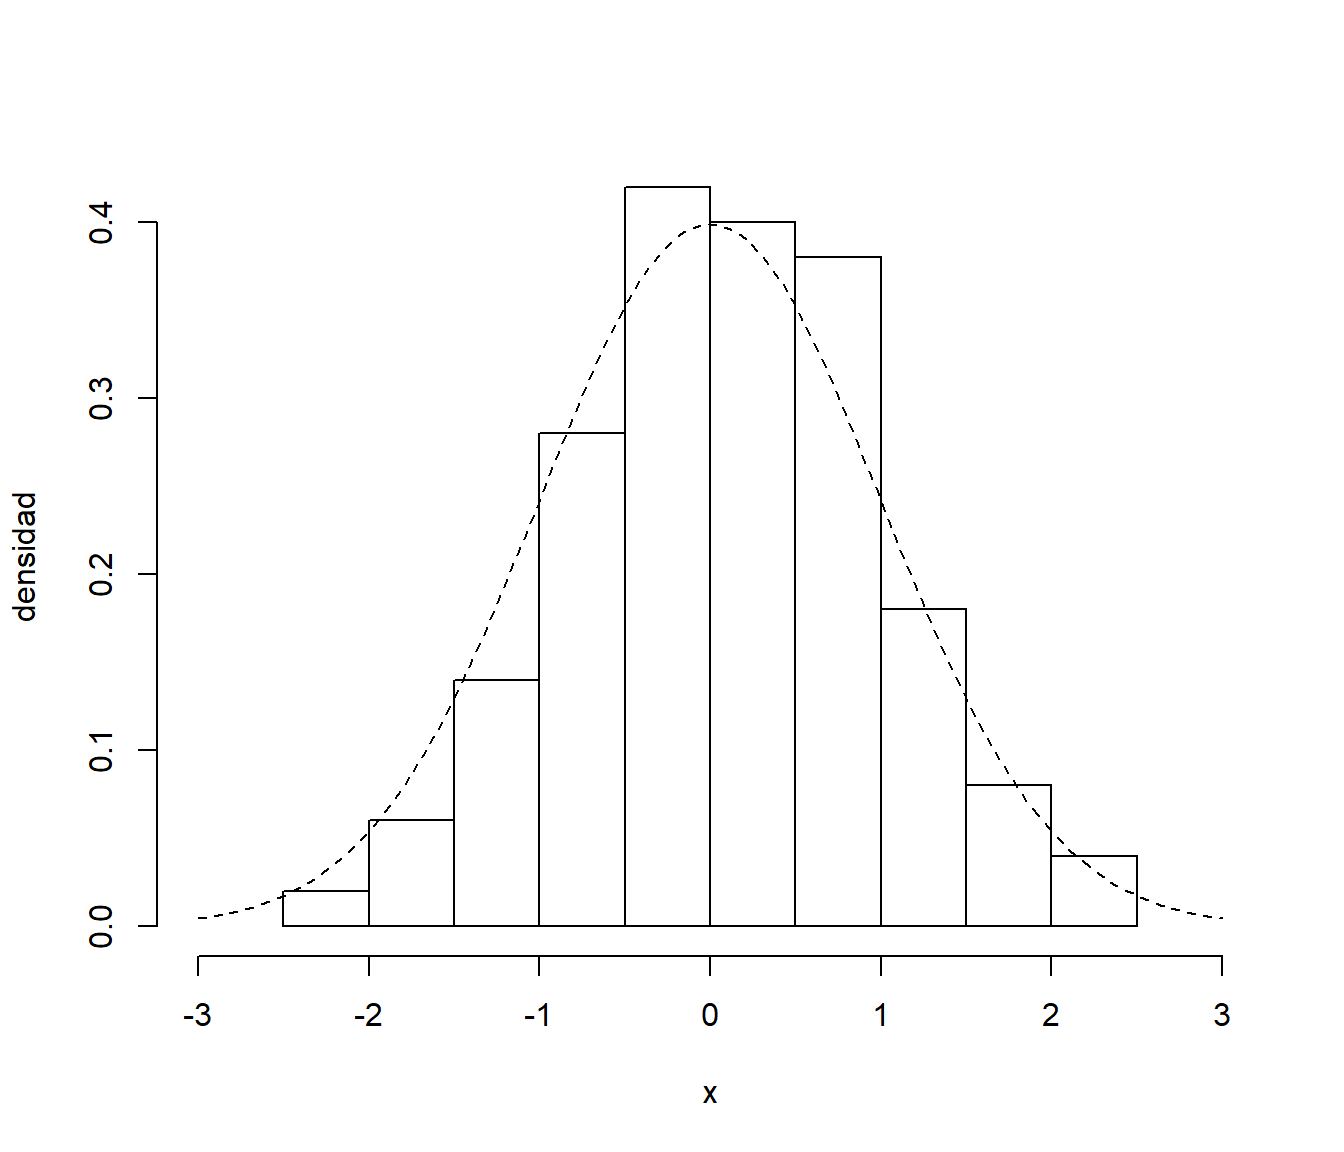
\includegraphics[width=0.7\linewidth]{01-intro_files/figure-latex/muestra-sim-1} 

}

\caption{Distribución de la muestra simulada.}\label{fig:muestra-sim}
\end{figure}

Como aproximación de la distribución poblacional, desconocida en la
práctica, siempre podemos considerar la distribución empírica (o una
versión suavizada: bootstrap suavizado; Sección \ref{cap4-boot-suav}).
Alternativamente podríamos asumir un modelo paramétrico y estimar los
parámetros a partir de la muestra {[}Figura
\ref{fig:muestra-sim-aprox}{]}.

\begin{Shaded}
\begin{Highlighting}[]
\CommentTok{# Distribución bootstrap uniforme}
\KeywordTok{curve}\NormalTok{(}\KeywordTok{ecdf}\NormalTok{(muestra)(x), }\DataTypeTok{xlim =} \KeywordTok{c}\NormalTok{(}\OperatorTok{-}\DecValTok{3}\NormalTok{, }\DecValTok{3}\NormalTok{), }\DataTypeTok{ylab =} \StringTok{"F(x)"}\NormalTok{, }\DataTypeTok{type =} \StringTok{"s"}\NormalTok{)}
\CommentTok{# Distribución bootstrap paramétrico (asumiendo normalidad)}
\KeywordTok{curve}\NormalTok{(}\KeywordTok{pnorm}\NormalTok{(x, }\KeywordTok{mean}\NormalTok{(muestra), }\KeywordTok{sd}\NormalTok{(muestra)), }\DataTypeTok{lty =} \DecValTok{2}\NormalTok{, }\DataTypeTok{add =} \OtherTok{TRUE}\NormalTok{)}
\CommentTok{# Distribución teórica}
\KeywordTok{curve}\NormalTok{(pnorm, }\DataTypeTok{lty =} \DecValTok{3}\NormalTok{, }\DataTypeTok{add =} \OtherTok{TRUE}\NormalTok{)}
\KeywordTok{legend}\NormalTok{(}\StringTok{"bottomright"}\NormalTok{, }\DataTypeTok{legend =} \KeywordTok{c}\NormalTok{(}\StringTok{"Empírica"}\NormalTok{, }\StringTok{"Aprox. paramétrica"}\NormalTok{, }\StringTok{"Teórica"), lty = 1:3)}
\end{Highlighting}
\end{Shaded}

\begin{figure}[!htb]

{\centering 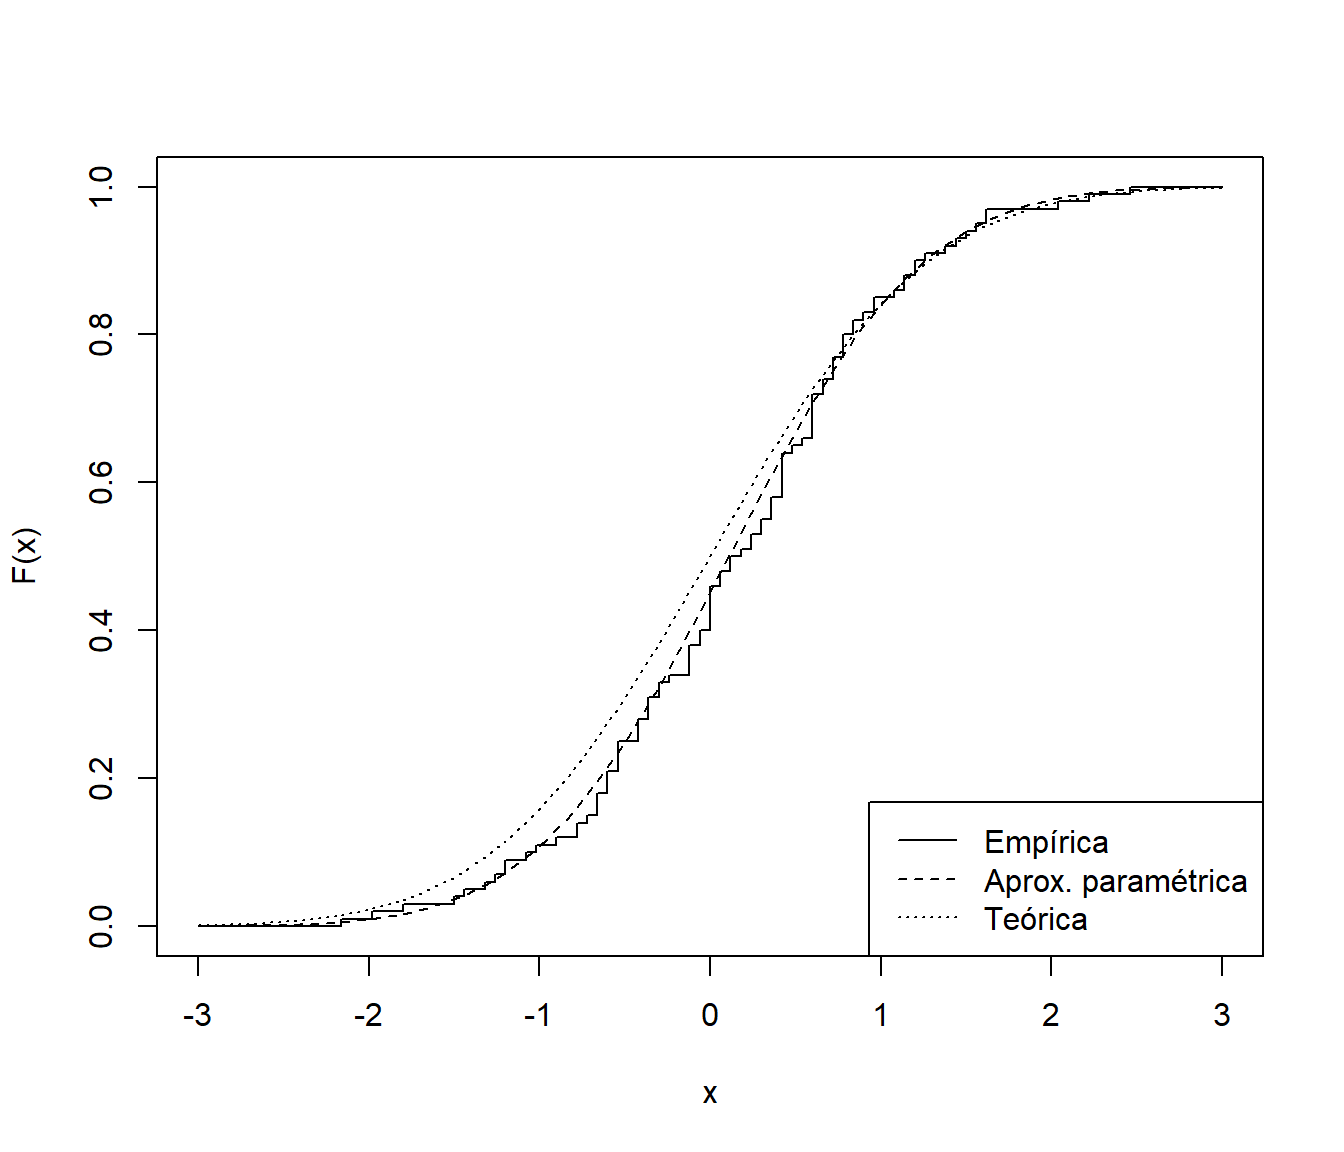
\includegraphics[width=0.7\linewidth]{01-intro_files/figure-latex/muestra-sim-aprox-1} 

}

\caption{Distribución teórica de la muestra simulada y distintas aproximaciones.}\label{fig:muestra-sim-aprox}
\end{figure}

A partir de la aproximación \(\hat{F}\) podríamos generar,
condicionalmente a la muestra observada, remuestras
\[\mathbf{X}^{\ast}=\left( X_1^{\ast},\ldots ,X_n^{\ast} \right)\] con
distribución \(X_i^{\ast} \sim \hat{F}\), que demoninaremos remuestras
bootstrap. Por lo que podemos hablar de la distribución en el remuestreo
de \[R^{\ast}=R\left( \mathbf{X}^{\ast},\hat{F} \right),\] llamada
distribución bootstrap.

La idea original (Efron, 1979) es que la distribución de
\(\hat{\theta}_{b}^{\ast }\) en torno a \(\hat{\theta}\) aproxima la
distribución de \(\hat{\theta}\) en torno a \(\theta\). Por tanto se
pretende aproximar la distribución en el muestreo de \(R\) por la
distribución bootstrap de \(R^{\ast}\).

En raras ocasiones la distribución bootstrap de \(R^{\ast}\) es
calculable directamente, pero siempre suele poder aproximarse por Monte
Carlo.

\subsection{Implementación en la práctica}\label{cap1-implementacion}

En el caso i.i.d., si empleamos como aproximación la distribución
empírica \(\hat{F}=F_n\), la generación de las muestras bootstrap puede
hacerse mediante remuestreo (manteniendo el tamaño muestral). Habría que
simular una muestra de tamaño \(n\) de una variable aleatoria discreta
que toma los valores \(X_1,\ldots ,X_n\) todos ellos con probabilidad
\(\frac{1}{n}\):

\begin{itemize}
\tightlist
\item
  Para cada \(i=1,\ldots, n\),
  \(P^{\ast}\left( X_i^{\ast}=X_j \right) =  \frac{1}{n}\),
  \(j=1,\ldots ,n\).
\end{itemize}

Existen multitud de algoritmos para simular variables discretas, pero en
este caso de equiprobabilidad hay un procedimiento muy eficiente (método
de la transformación cuantil con búsqueda directa) que se reduce a
simular un número aleatorio \(U\), con distribución
\(\mathcal{U}\left( 0,1 \right)\), y hacer
\(X^{\ast}=X_{\left\lfloor nU\right\rfloor +1}\), donde
\(\left\lfloor x\right\rfloor\) representa la parte entera de \(x\), es
decir, el mayor número entero que sea menor o igual que \(x\). Empleando
ese método, el procedimiento para generar la muestra bootstrap sería:

\begin{itemize}
\tightlist
\item
  Para cada \(i=1,\ldots ,n\) generar
  \(U_i\sim \mathcal{U}\left( 0,1 \right)\) y hacer
  \(X_i^{\ast}=X_{\left\lfloor nU_i\right\rfloor +1}\).
\end{itemize}

\begin{Shaded}
\begin{Highlighting}[]
\KeywordTok{set.seed}\NormalTok{(}\DecValTok{1}\NormalTok{)}
\NormalTok{n <-}\StringTok{ }\KeywordTok{length}\NormalTok{(muestra)}
\NormalTok{u <-}\StringTok{ }\KeywordTok{runif}\NormalTok{(n)}
\NormalTok{muestra_boot <-}\StringTok{ }\NormalTok{muestra[}\KeywordTok{floor}\NormalTok{(n}\OperatorTok{*}\NormalTok{u) }\OperatorTok{+}\StringTok{ }\DecValTok{1}\NormalTok{]}
\KeywordTok{head}\NormalTok{(muestra_boot)}
\end{Highlighting}
\end{Shaded}

\begin{verbatim}
## [1] -0.1557955 -0.0593134 -1.0441346 -0.5425200  0.9189774  0.2670988
\end{verbatim}

En \texttt{R} es recomendable\footnote{De esta forma se evitan posibles
  problemas numéricos al emplear el método de la transformación cuantil
  cuando \(n\) es extremadamente grande (e.g.
  \url{https://stat.ethz.ch/pipermail/r-devel/2018-September/076817.html}).}
emplear la función \texttt{sample} para generar muestras aleatorias con
reemplazamiento del conjunto de datos original:

\begin{Shaded}
\begin{Highlighting}[]
\NormalTok{muestra_boot <-}\StringTok{ }\KeywordTok{sample}\NormalTok{(muestra, }\DataTypeTok{replace =} \OtherTok{TRUE}\NormalTok{)}
\KeywordTok{head}\NormalTok{(muestra_boot)}
\end{Highlighting}
\end{Shaded}

\begin{verbatim}
## [1]  0.18879230 -0.41499456 -1.47075238 -0.47340064  0.02800216  0.78213630
\end{verbatim}

En el caso multidimensional, cuando trabajamos con un conjunto de datos
con múltiples variables, podríamos emplear un procedimiento análogo, a
partir de remuestras del vector de índices. Por ejemplo:

\begin{Shaded}
\begin{Highlighting}[]
\KeywordTok{data}\NormalTok{(iris)}
\KeywordTok{str}\NormalTok{(iris)}
\end{Highlighting}
\end{Shaded}

\begin{verbatim}
## 'data.frame':    150 obs. of  5 variables:
##  $ Sepal.Length: num  5.1 4.9 4.7 4.6 5 5.4 4.6 5 4.4 4.9 ...
##  $ Sepal.Width : num  3.5 3 3.2 3.1 3.6 3.9 3.4 3.4 2.9 3.1 ...
##  $ Petal.Length: num  1.4 1.4 1.3 1.5 1.4 1.7 1.4 1.5 1.4 1.5 ...
##  $ Petal.Width : num  0.2 0.2 0.2 0.2 0.2 0.4 0.3 0.2 0.2 0.1 ...
##  $ Species     : Factor w/ 3 levels "setosa","versicolor",..: 1 1 1 1 1 1 1 1 1 1 ...
\end{verbatim}

\begin{Shaded}
\begin{Highlighting}[]
\NormalTok{n <-}\StringTok{ }\KeywordTok{nrow}\NormalTok{(iris)}
\CommentTok{# i_boot <- floor(n*runif(n)) + 1}
\CommentTok{# i_boot <- sample.int(n, replace = TRUE)}
\NormalTok{i_boot <-}\StringTok{ }\KeywordTok{sample}\NormalTok{(n, }\DataTypeTok{replace =} \OtherTok{TRUE}\NormalTok{)}
\NormalTok{data_boot <-}\StringTok{ }\NormalTok{iris[i_boot, ]}
\KeywordTok{str}\NormalTok{(data_boot)}
\end{Highlighting}
\end{Shaded}

\begin{verbatim}
## 'data.frame':    150 obs. of  5 variables:
##  $ Sepal.Length: num  5 5.2 6.7 5 5.2 6.7 5.4 5.1 4.4 7.3 ...
##  $ Sepal.Width : num  3.5 4.1 3 3.5 3.5 3 3 3.8 3 2.9 ...
##  $ Petal.Length: num  1.3 1.5 5 1.3 1.5 5 4.5 1.5 1.3 6.3 ...
##  $ Petal.Width : num  0.3 0.1 1.7 0.3 0.2 1.7 1.5 0.3 0.2 1.8 ...
##  $ Species     : Factor w/ 3 levels "setosa","versicolor",..: 1 1 2 1 1 2 2 1 1 3 ...
\end{verbatim}

Esta forma de proceder es la que emplea por defecto el paquete
\texttt{boot} que describiremos más adelante (Sección
\ref{cap1-pkgboot}).

\BeginKnitrBlock{example}[Inferencia sobre la media con varianza conocida]
\protect\hypertarget{exm:media-dt-conocida}{}{\label{exm:media-dt-conocida}
\iffalse (Inferencia sobre la media con varianza conocida) \fi{} }
\vspace{0.5cm}

Hemos observado 15 tiempos de vida de microorganismos: 0.143, 0.182,
0.256, 0.260, 0.270, 0.437, 0.509, 0.611, 0.712, 1.04, 1.09, 1.15, 1.46,
1.88, 2.08. A partir de los cuales queremos obtener una estimación por
intervalo de confianza de su vida media, suponiendo que la desviación
típica es conocida e igual a 0.6 (en el Capítulo \ref{cap5} se tratará
con más detalle la construcción de intervalos de confianza).
\EndKnitrBlock{example}

\begin{Shaded}
\begin{Highlighting}[]
\NormalTok{muestra <-}\StringTok{ }\KeywordTok{c}\NormalTok{(}\FloatTok{0.143}\NormalTok{, }\FloatTok{0.182}\NormalTok{, }\FloatTok{0.256}\NormalTok{, }\FloatTok{0.26}\NormalTok{, }\FloatTok{0.27}\NormalTok{, }\FloatTok{0.437}\NormalTok{, }\FloatTok{0.509}\NormalTok{, }
    \FloatTok{0.611}\NormalTok{, }\FloatTok{0.712}\NormalTok{, }\FloatTok{1.04}\NormalTok{, }\FloatTok{1.09}\NormalTok{, }\FloatTok{1.15}\NormalTok{, }\FloatTok{1.46}\NormalTok{, }\FloatTok{1.88}\NormalTok{, }\FloatTok{2.08}\NormalTok{)}
\NormalTok{sigma <-}\StringTok{ }\FloatTok{0.6}
\KeywordTok{summary}\NormalTok{(muestra)}
\end{Highlighting}
\end{Shaded}

\begin{verbatim}
##    Min. 1st Qu.  Median    Mean 3rd Qu.    Max. 
##  0.1430  0.2650  0.6110  0.8053  1.1200  2.0800
\end{verbatim}

\begin{Shaded}
\begin{Highlighting}[]
\KeywordTok{sd}\NormalTok{(muestra)}
\end{Highlighting}
\end{Shaded}

\begin{verbatim}
## [1] 0.6237042
\end{verbatim}

\begin{Shaded}
\begin{Highlighting}[]
\KeywordTok{hist}\NormalTok{(muestra)}
\KeywordTok{rug}\NormalTok{(muestra)}
\end{Highlighting}
\end{Shaded}

\begin{figure}[!htb]

{\centering 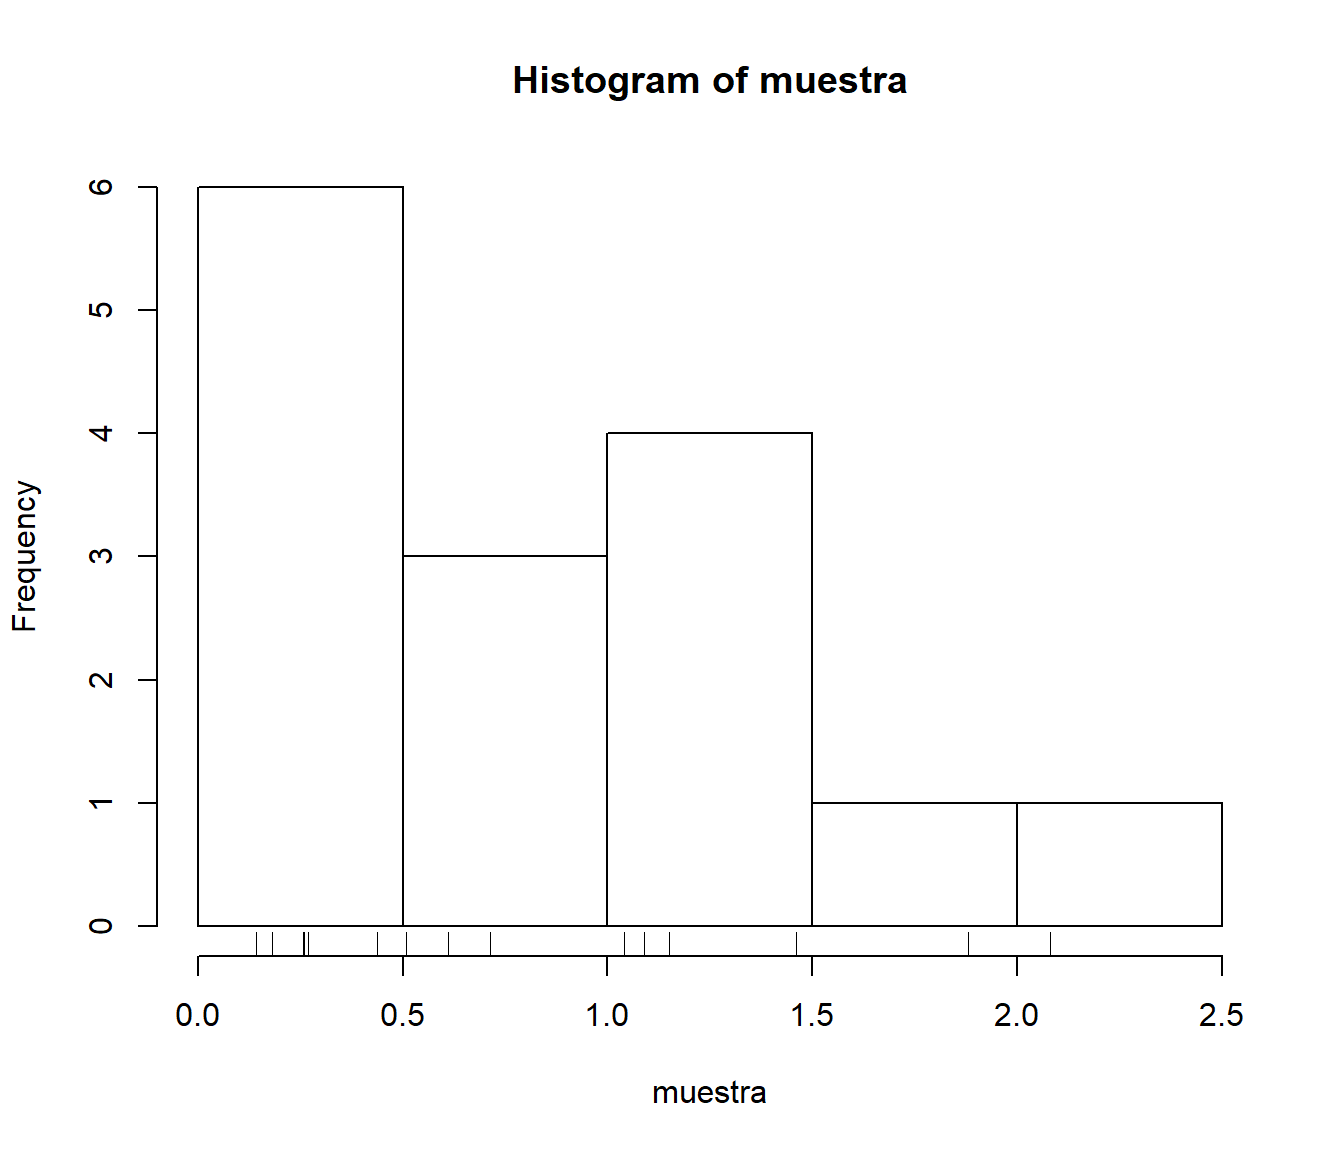
\includegraphics[width=0.7\linewidth]{01-intro_files/figure-latex/microorganismos-1} 

}

\caption{Distribución del tiempo de vida de microorganismos.}\label{fig:microorganismos}
\end{figure}

{[}Figura \ref{fig:microorganismos}{]}

\textbf{\emph{Contexto clásico}}

Suponemos que los datos \(\mathbf{X}=\left( X_1,\ldots ,X_n \right)\)
son una m.a.s. de una población con distribución \(F\), con \(\mu\)
desconocida y \(\sigma\) conocida, y que estamos interesados en hacer
inferencia sobre:
\[\theta \left( F \right) =\mu =\int x~dF\left( x \right)\] Para ello,
un estadístico adecuado para este caso es:
\[R=R\left( \mathbf{X},F \right) =\sqrt{n}\frac{\bar{X}-\mu }{\sigma},\]
con
\(\theta \left( F_n \right) =\int x~dF_n\left( x \right) = \bar{X}\).

Bajo normalidad
\(\left( X\sim \mathcal{N}\left( \mu ,\sigma^2 \right) \right)\),
\(R\sim N\left( 0,1 \right)\). Si \(F\) no es normal, tan sólo sabemos
que, bajo ciertas condiciones,
\(R\overset{d}{\rightarrow }\mathcal{N}\left( 0, 1 \right)\).

A partir de esta última aproximación, se obtiene el intervalo de
confianza asintótico (de nivel \(1-\alpha\)) para la media \(\mu\):
\[\hat{IC}_{1-\alpha}\left(  \mu\right)  = 
\left(  \overline{X}-z_{1-\alpha/2}\dfrac{\sigma}{\sqrt{n}},\ \overline{X} 
+ z_{1-\alpha/2}\dfrac{\sigma}{\sqrt{n}} \right).\]

\begin{Shaded}
\begin{Highlighting}[]
\NormalTok{alfa <-}\StringTok{ }\FloatTok{0.05}
\NormalTok{x_barra <-}\StringTok{ }\KeywordTok{mean}\NormalTok{(muestra)}
\NormalTok{z <-}\StringTok{ }\KeywordTok{qnorm}\NormalTok{(}\DecValTok{1} \OperatorTok{-}\StringTok{ }\NormalTok{alfa}\OperatorTok{/}\DecValTok{2}\NormalTok{)}
\NormalTok{ic_inf <-}\StringTok{ }\NormalTok{x_barra }\OperatorTok{-}\StringTok{ }\NormalTok{z}\OperatorTok{*}\NormalTok{sigma}\OperatorTok{/}\KeywordTok{sqrt}\NormalTok{(n)}
\NormalTok{ic_sup <-}\StringTok{ }\NormalTok{x_barra }\OperatorTok{+}\StringTok{ }\NormalTok{z}\OperatorTok{*}\NormalTok{sigma}\OperatorTok{/}\KeywordTok{sqrt}\NormalTok{(n)}
\NormalTok{IC <-}\StringTok{ }\KeywordTok{c}\NormalTok{(ic_inf, ic_sup)}
\NormalTok{IC}
\end{Highlighting}
\end{Shaded}

\begin{verbatim}
## [1] 0.7093151 0.9013516
\end{verbatim}

\textbf{\emph{Contexto bootstrap}}

Consideramos la función de distribución empírica \(\hat{F}=F_n\) como
aproximación de la distribución poblacional (bootstrap uniforme). Para
aproximar la distribución bootstrap del estadístico por Monte Carlo, se
generan \(B=1000\) muestras bootstrap
\(\mathbf{X}^{\ast (b)}=\left( X_1^{\ast (b)},\ldots ,X_n^{\ast (b)} \right)\)
de forma que
\(P^{\ast (b)}\left( X_i^{\ast}=X_j \right) = \frac{1}{n}\),
\(j=1,\ldots ,n\), para \(i=1,\ldots, n\) y \(b=1,\ldots, B\). A partir
de las cuales se obtienen las \(B\) réplicas bootstrap del estadístico:
\[R^{\ast (b)}=R\left( \mathbf{X}^{\ast (b)},\hat{F} \right) =\sqrt{n}\frac{
\bar{X}^{\ast  (b)}-\bar{X}}{\sigma }, \ b=1,\ldots, B, \] con
\(\bar{X}^{\ast (b)} = \frac{1}{n}\sum X_i^{\ast (b)}\).

\begin{Shaded}
\begin{Highlighting}[]
\KeywordTok{set.seed}\NormalTok{(}\DecValTok{1}\NormalTok{)}
\NormalTok{B <-}\StringTok{ }\DecValTok{1000}
\NormalTok{estadistico_boot <-}\StringTok{ }\KeywordTok{numeric}\NormalTok{(B)}
\ControlFlowTok{for}\NormalTok{ (k }\ControlFlowTok{in} \DecValTok{1}\OperatorTok{:}\NormalTok{B) \{}
\NormalTok{    remuestra <-}\StringTok{ }\KeywordTok{sample}\NormalTok{(muestra, n, }\DataTypeTok{replace =} \OtherTok{TRUE}\NormalTok{)}
\NormalTok{    x_barra_boot <-}\StringTok{ }\KeywordTok{mean}\NormalTok{(remuestra)}
\NormalTok{    estadistico_boot[k] <-}\StringTok{ }\KeywordTok{sqrt}\NormalTok{(n) }\OperatorTok{*}\StringTok{ }\NormalTok{(x_barra_boot }\OperatorTok{-}\StringTok{ }\NormalTok{x_barra)}\OperatorTok{/}\NormalTok{sigma}
\NormalTok{\}}
\end{Highlighting}
\end{Shaded}

Las características de interés de la distribución en el muestreo de
\(R\) se aproximan por las correspondientes de la distribución bootstrap
de \(R^{\ast}\). En este caso nos interesa aproximar los puntos críticos
\(x_{\alpha /2}\) y \(x_{1-\alpha /2}\), tales que:
\[P\left( x_{\alpha /2} < R < x_{1-\alpha /2} \right) = 1-\alpha.\] Para
lo que podemos emplear los cuantiles muestrales\footnote{Se podrían
  considerar distintos estimadores del cuantil \(x_{\alpha}\) (ver p.e.
  la ayuda de la función \texttt{quantile()}). Si empleamos directamente
  la distribución empírica, el cuantil se correspondería con la
  observación ordenada en la posición \(B \alpha\) (se suele hacer una
  interpolación lineal si este valor no es entero), lo que equivale a
  emplear la función \texttt{quantile()} de \texttt{R} con el parámetro
  \texttt{type\ =\ 1}. Esta función considera por defecto la posición
  \(1 + (B - 1) \alpha\) (\texttt{type\ =\ 7}). En el libro de Davison y
  Hinkley (1997), y en el paquete \texttt{boot}, se emplea
  \((B + 1) \alpha\) (equivalente a \texttt{type\ =\ 6}; lo que
  justifica que consideren habitualmente 99, 199 ó 999 réplicas
  bootstrap).}:

\begin{Shaded}
\begin{Highlighting}[]
\CommentTok{# Empleando la distribución empírica del estadístico bootstrap: }
\NormalTok{estadistico_boot_ordenado <-}\StringTok{ }\KeywordTok{sort}\NormalTok{(estadistico_boot)}
\NormalTok{indice_inf <-}\StringTok{ }\KeywordTok{floor}\NormalTok{(B }\OperatorTok{*}\StringTok{ }\NormalTok{alfa}\OperatorTok{/}\DecValTok{2}\NormalTok{)}
\NormalTok{indice_sup <-}\StringTok{ }\KeywordTok{floor}\NormalTok{(B }\OperatorTok{*}\StringTok{ }\NormalTok{(}\DecValTok{1} \OperatorTok{-}\StringTok{ }\NormalTok{alfa}\OperatorTok{/}\DecValTok{2}\NormalTok{))}
\NormalTok{pto_crit <-}\StringTok{ }\NormalTok{estadistico_boot_ordenado[}\KeywordTok{c}\NormalTok{(indice_inf, indice_sup)]}
\CommentTok{# Empleando la función `quantile`:}
\CommentTok{# pto_crit <- quantile(estadistico_boot, c(alfa/2, 1 - alfa/2), type = 1)}
\NormalTok{pto_crit <-}\StringTok{ }\KeywordTok{quantile}\NormalTok{(estadistico_boot, }\KeywordTok{c}\NormalTok{(alfa}\OperatorTok{/}\DecValTok{2}\NormalTok{, }\DecValTok{1} \OperatorTok{-}\StringTok{ }\NormalTok{alfa}\OperatorTok{/}\DecValTok{2}\NormalTok{))}
\NormalTok{pto_crit}
\end{Highlighting}
\end{Shaded}

\begin{verbatim}
##      2.5%     97.5% 
## -1.851858  1.873377
\end{verbatim}

A partir de los cuales obtenemos la correspondiente estimación por IC
boostrap: \[\hat{IC}^{boot}_{1-\alpha}\left(  \mu\right)  = 
\left(  \overline{X}-x_{1-\alpha/2}\dfrac{\sigma}{\sqrt{n}},\ \overline{X} 
- x_{\alpha/2}\dfrac{\sigma}{\sqrt{n}} \right).\]

\begin{Shaded}
\begin{Highlighting}[]
\CommentTok{# Construcción del IC}
\NormalTok{ic_inf_boot <-}\StringTok{ }\NormalTok{x_barra }\OperatorTok{-}\StringTok{ }\NormalTok{pto_crit[}\DecValTok{2}\NormalTok{] }\OperatorTok{*}\StringTok{ }\NormalTok{sigma}\OperatorTok{/}\KeywordTok{sqrt}\NormalTok{(n)}
\NormalTok{ic_sup_boot <-}\StringTok{ }\NormalTok{x_barra }\OperatorTok{-}\StringTok{ }\NormalTok{pto_crit[}\DecValTok{1}\NormalTok{] }\OperatorTok{*}\StringTok{ }\NormalTok{sigma}\OperatorTok{/}\KeywordTok{sqrt}\NormalTok{(n)}
\NormalTok{IC_boot <-}\StringTok{ }\KeywordTok{c}\NormalTok{(ic_inf_boot, ic_sup_boot)}
\KeywordTok{names}\NormalTok{(IC_boot) <-}\StringTok{ }\KeywordTok{paste0}\NormalTok{(}\DecValTok{100}\OperatorTok{*}\KeywordTok{c}\NormalTok{(alfa}\OperatorTok{/}\DecValTok{2}\NormalTok{, }\DecValTok{1}\OperatorTok{-}\NormalTok{alfa}\OperatorTok{/}\DecValTok{2}\NormalTok{), }\StringTok{"%"}\NormalTok{) }\CommentTok{# rev(names(IC_boot))}
\NormalTok{IC_boot}
\end{Highlighting}
\end{Shaded}

\begin{verbatim}
##      2.5%     97.5% 
## 0.7135570 0.8960555
\end{verbatim}

Nótese que este intervalo de confianza no está centrado en la media, al
contrario que el obtenido con la aproximación tradicional. Aunque en
este caso no se observan grandes diferencias ya que la distribución
bootstrap obtenida es muy similar a la aproximación normal (ver Figura
\ref{fig:estad-boot}).

\begin{Shaded}
\begin{Highlighting}[]
\KeywordTok{hist}\NormalTok{(estadistico_boot, }\DataTypeTok{freq =} \OtherTok{FALSE}\NormalTok{)}
\KeywordTok{lines}\NormalTok{(}\KeywordTok{density}\NormalTok{(estadistico_boot))}
\KeywordTok{abline}\NormalTok{(}\DataTypeTok{v =}\NormalTok{ pto_crit)}
\KeywordTok{curve}\NormalTok{(dnorm, }\DataTypeTok{lty =} \DecValTok{2}\NormalTok{, }\DataTypeTok{add =} \OtherTok{TRUE}\NormalTok{)}
\KeywordTok{abline}\NormalTok{(}\DataTypeTok{v =} \KeywordTok{c}\NormalTok{(}\OperatorTok{-}\NormalTok{z, z), }\DataTypeTok{lty =} \DecValTok{2}\NormalTok{)}
\end{Highlighting}
\end{Shaded}

\begin{figure}[!htb]

{\centering 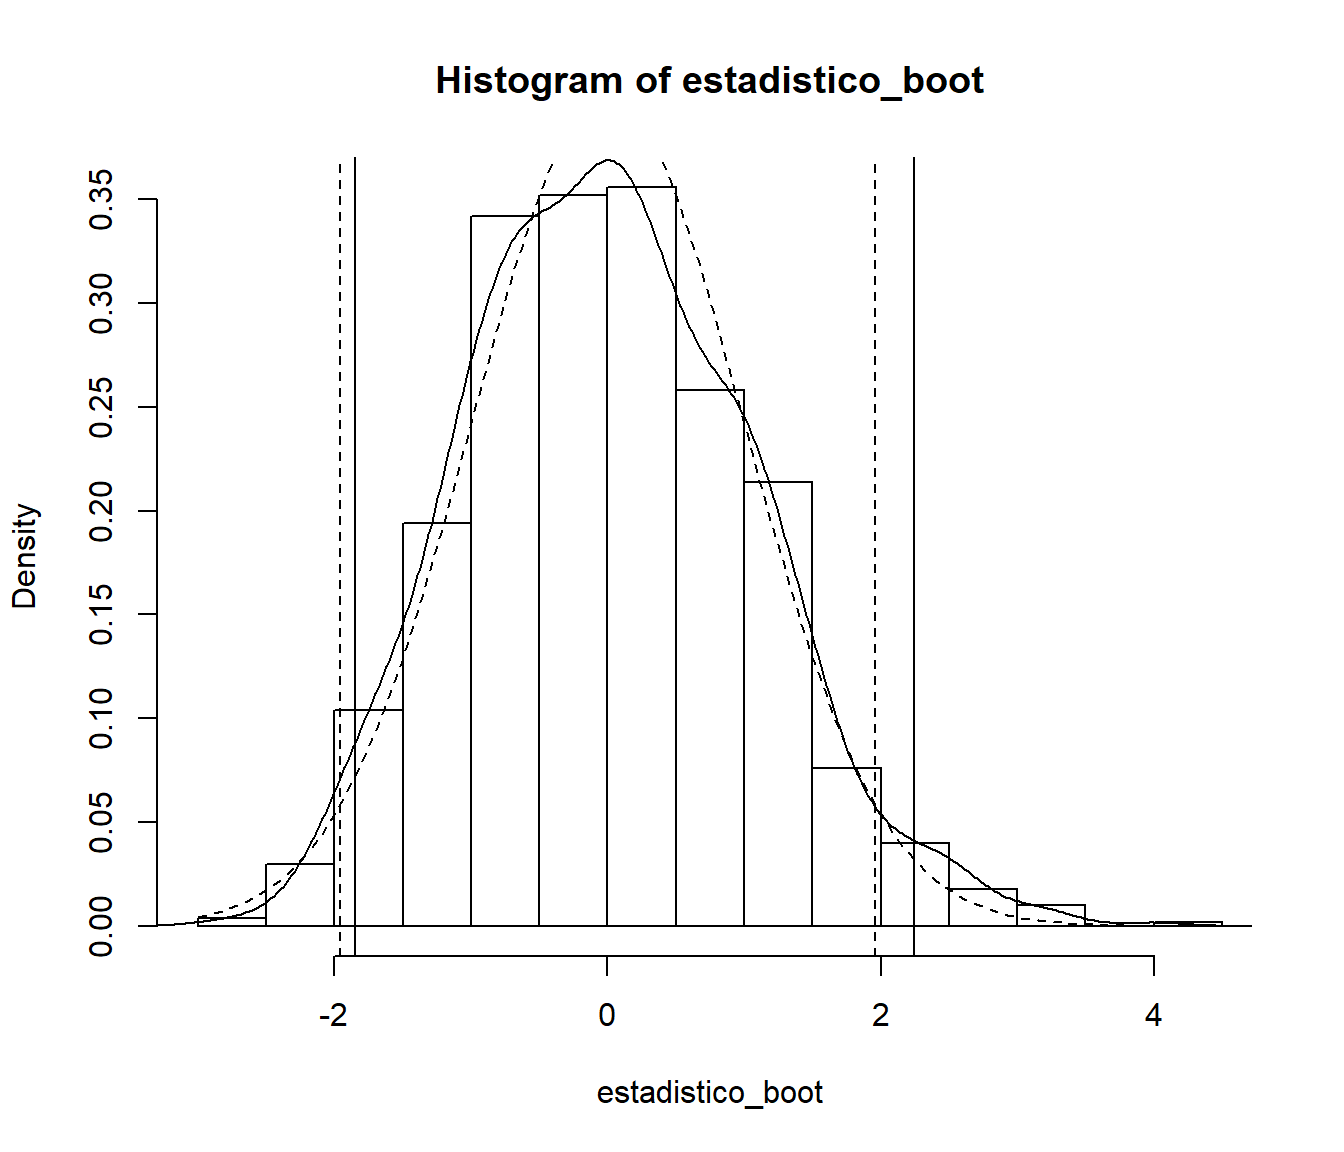
\includegraphics[width=0.7\linewidth]{01-intro_files/figure-latex/estad-boot-1} 

}

\caption{Distribución del estadístico boostrap y aproximaciones de los cuantiles. Con línea discontinua se muestra la distribución normal asintótica.}\label{fig:estad-boot}
\end{figure}

\section{El Bootstrap uniforme}\label{cap1-unif}

Como ya se comentó anteriormente el bootstrap uniforme es aquel en el
que se reemplaza la distribución poblacional (desconocida) por la
distribución empírica:
\[F_n\left( x \right) =\frac{1}{n}\sum_{i=1}^{n}\mathbf{1}\left\{ X_i\leq x\right\}.\]

Es decir \(\hat{F}=F_n\) y, por lo tanto,
\(R^{\ast}=R\left( \mathbf{X}^{\ast},F_n \right)\).

Conviene recordar algunas propiedades de la distribución empírica:
\[\begin{aligned}
nF_n\left( x \right) &= \sum_{i=1}^{n}\mathbf{1}\left\{ X_i\leq x\right\}
\sim \mathcal{B}\left( n,F\left( x \right) \right), \\
E\left( nF_n\left( x \right) \right) &= nF\left( x \right) \implies E\left(
F_n\left( x \right) \right) =F\left( x \right), \\
Var\left( nF_n\left( x \right) \right) &=  nF\left( x \right) \left(
1-F\left( x \right) \right) \\
&\implies  Var\left( F_n\left( x \right) \right) =\frac{F\left( x \right) \left( 1-F\left( x \right) \right)}{n}
\end{aligned}\]

Así pues, en este caso el algoritmo bootstrap uniforme (también llamado
bootstrap naïve) es el siguiente:

\begin{enumerate}
\def\labelenumi{\arabic{enumi}.}
\item
  Para cada \(i=1,\ldots ,n\) arrojar \(X_i^{\ast}\) a partir de
  \(F_n\), es decir
  \(P^{\ast}\left( X_i^{\ast}=X_j \right) =\frac{1}{n}\),
  \(j=1,\ldots ,n\)
\item
  Obtener
  \(\mathbf{X}^{\ast}=\left( X_1^{\ast},\ldots ,X_n^{\ast} \right)\)
\item
  Calcular \(R^{\ast}=R\left( \mathbf{X}^{\ast},F_n \right)\)
\end{enumerate}

Como veremos más adelante, a veces (muy poco frecuentemente) es posible
calcular exactamente la distribución bootstrap de \(R^{\ast}\). Cuando
eso no es posible, esa distribución es fácilmente aproximable por Monte
Carlo, arrojando una gran cantidad, \(B\), de réplicas de \(R^{\ast}\).
En ese caso, el algoritmo se convierte en:

\begin{enumerate}
\def\labelenumi{\arabic{enumi}.}
\item
  Para cada \(i=1,\ldots ,n\) arrojar \(X_i^{\ast}\) a partir de \(F_n\)
\item
  Obtener
  \(\mathbf{X}^{\ast}=\left( X_1^{\ast},\ldots ,X_n^{\ast} \right)\)
\item
  Calcular \(R^{\ast}=R\left( \mathbf{X}^{\ast},F_n \right)\)
\item
  Repetir \(B\) veces los pasos 1-3 para obtener las réplicas bootstrap
  \(R^{\ast (1)}, \ldots, R^{\ast (B)}\)
\item
  Utilizar esas réplicas bootstrap para aproximar la distribución en el
  muestreo de \(R\)
\end{enumerate}

\subsection{Ejemplos}\label{ejemplos}

\BeginKnitrBlock{example}[Inferencia sobre la media con varianza conocida, continuación]
\protect\hypertarget{exm:media-dt-conocida-perturbando}{}{\label{exm:media-dt-conocida-perturbando}
\iffalse (Inferencia sobre la media con varianza conocida, continuación)
\fi{} }
\EndKnitrBlock{example}

En el Ejemplo \ref{exm:media-dt-conocida} anteriormente visto de
inferencia para la media con varianza conocida, el algoritmo bootstrap
(basado en Monte Carlo) para aproximar la distribución en el muestreo de
\(R\) empleado fue:

\begin{enumerate}
\def\labelenumi{\arabic{enumi}.}
\item
  Para cada \(i=1,\ldots ,n\) arrojar
  \(U_i\sim \mathcal{U}\left( 0,1 \right)\) y hacer
  \(X_i^{\ast}=X_{\left\lfloor nU_i\right\rfloor +1}\)
\item
  Obtener \(\bar{X}^{\ast}=\frac{1}{n}\sum X_i^{\ast}\)
\item
  Calcular \(R^{\ast}=\sqrt{n}\frac{\bar{X}^{\ast}-\bar{X}}{ \sigma }\)
\item
  Repetir \(B\) veces los pasos 1-3 para obtener las réplicas bootstrap
  \(R^{\ast (1)}, \ldots, R^{\ast (B)}\)
\item
  Aproximar la distribución en el muestreo de \(R\) mediante la empírica
  de \(R^{\ast (1)}, \ldots, R^{\ast (B)}\)
\end{enumerate}

Como curiosidad podemos calcular la esperanza y la varianza de \(R\) y
la esperanza y varianza bootstrap de \(R^{\ast}\). Para \(R\) tenemos:
\[\begin{aligned}
E\left( R \right) &=\sqrt{n}\frac{E\left( \bar{X} \right) -\mu }{\sigma }
=0, \\
Var\left( R \right) &=n\frac{Var\left( \bar{X} \right)}{\sigma^2}=n
\frac{\frac{1}{n}\sigma^2}{\sigma^2}=1.
\end{aligned}\]

Para calcular esos mismos momentos de \(R^{\ast}\), resultará útil
obtener previamente la esperanza y varianza bootstrap de
\(\bar{X}^{\ast}\): \[\begin{aligned}
E^{\ast}\left( \bar{X}^{\ast} \right) &= \frac{1}{n}
\sum_{i=1}^{n}E^{\ast}\left( X_i^{\ast} \right) =\frac{1}{n}
\sum_{i=1}^{n}E^{\ast}\left( X_1^{\ast} \right) =E^{\ast}\left(
X_1^{\ast} \right) =\bar{X}, \\
Var^{\ast}\left( \bar{X}^{\ast} \right) &= \frac{1}{n^2}
\sum_{i=1}^{n}Var^{\ast}\left( X_i^{\ast} \right) =\frac{1}{n^2}
\sum_{i=1}^{n}Var^{\ast}\left( X_1^{\ast} \right) =\frac{1}{n}Var^{\ast
}\left( X_1^{\ast} \right) =\frac{S_n^2}{n},
\end{aligned}\] ya que \[\begin{aligned}
E^{\ast}\left( X_1^{\ast} \right) &= \sum_{j=1}^{n}X_jP^{\ast}\left(
X_1^{\ast}=X_j \right) =\sum_{j=1}^{n}\frac{1}{n}X_j=\bar{X}, \\
Var^{\ast}\left( X_1^{\ast} \right) &= E^{\ast}\left( X_1^{\ast
2} \right) -\left[ E^{\ast}\left( X_1^{\ast} \right) \right]
^2=\sum_{j=1}^{n}X_j^2P^{\ast}\left( X_1^{\ast}=X_j \right) -\bar{X}
^2 \\
&= \frac{1}{n}\sum_{j=1}^{n}X_j^2-\bar{X}^2=\frac{1}{n}
\sum_{j=1}^{n}\left( X_j-\bar{X} \right)^2=S_n^2
\end{aligned}\]

Así pues, la esperanza y la varianza bootstrap de \(R^{\ast}\) resultan:
\[\begin{aligned}
E^{\ast}\left( R^{\ast} \right) &= \sqrt{n}\frac{E^{\ast}\left( \bar{X}^{\ast} \right) -\bar{X}}{\sigma }=0, \\
Var^{\ast}\left( R^{\ast} \right) &= n\frac{Var^{\ast}\left( \bar{X}^{\ast} \right)}{\sigma^2}=n\frac{\frac{1}{n}S_n^2}{\sigma^2}=
\frac{S_n^2}{\sigma^2}.
\end{aligned}\]

Es curioso observar que la esperanza de \(R\) y la esperanza bootstrap
de \(R^{\ast}\) coinciden (son ambas cero), pero no ocurre lo mismo con
sus varianzas: la de \(R\) es \(1\) y la varianza bootstrap de
\(R^{\ast}\) es \(S_n^2/\sigma^2\), que, aunque tiende a \(1\) (en
probabilidad o de forma casi segura, bajo las condiciones adecuadas)
cuando \(n\rightarrow \infty\), no es igual a \(1\). Eso nos lleva a
intuir que el método de remuestreo bootstrap propuesto quizá podría
modificarse ligeramente para que imitase exactamente al caso no
bootstrap también en la varianza. Puede comprobarse que eso se consigue
remuestreando \(X^{\ast}\) de la distribución empírica de la muestra
modificada: \(\left( \tilde{X}_1,\ldots ,\tilde{X}_n \right)\), siendo
\[\tilde{X}_i=\bar{X}+\frac{\sigma }{S_n}\left( X_i-\bar{X}
 \right) \text{, }i=1,\ldots ,n.\]

Efectivamente, bajo ese nuevo remuestreo, se tiene \[\begin{aligned}
E^{\ast}\left( \bar{X}^{\ast} \right) &= E^{\ast}\left( X_1^{\ast
} \right) =\overline{\tilde{X}}=\frac{1}{n}\sum_{i=1}^{n}\left[ \bar{X}+
\frac{\sigma }{S_n}\left( X_i-\bar{X} \right) \right] \\
&= \bar{X}+\frac{1}{n}\frac{\sigma }{S_n}\sum_{i=1}^{n}\left( X_i-
\bar{X} \right) =\bar{X}, \\
Var^{\ast}\left( \bar{X}^{\ast} \right) &= \frac{1}{n}Var^{\ast
}\left( X_1^{\ast} \right) =\frac{\sigma^2}{n},
\end{aligned}\] ya que \[\begin{aligned}
Var^{\ast}\left( X_1^{\ast} \right) &= E^{\ast}\left( X_1^{\ast
2} \right) -\left[ E^{\ast}\left( X_1^{\ast} \right) \right]
^2=\sum_{j=1}^{n}\tilde{X}_j^2P^{\ast}\left( X_1^{\ast}=\tilde{X}
_j \right) -\overline{\tilde{X}}^2 \\
&= \frac{1}{n}\sum_{j=1}^{n}\tilde{X}_j^2-\overline{\tilde{X}}^2=\frac{
1}{n}\sum_{j=1}^{n}\left( \tilde{X}_j-\overline{\tilde{X}} \right)^2=
\frac{1}{n}\sum_{j=1}^{n}\left[ \frac{\sigma }{S_n}\left( X_j-\bar{X} \right) \right]^2 \\
&= \frac{\sigma^2}{S_n^2}\frac{1}{n}\sum_{j=1}^{n}\left( X_i-
\bar{X} \right)^2=\frac{\sigma^2}{S_n^2}S_n^2=\sigma^2.
\end{aligned}\] Como consecuencia \[\begin{aligned}
E^{\ast}\left( R^{\ast} \right) &= \sqrt{n}\frac{E^{\ast}\left( 
\bar{X}^{\ast} \right) -\bar{X}}{\sigma }=0, \\
Var^{\ast}\left( R^{\ast} \right) &= n\frac{Var^{\ast}\left( 
\bar{X}^{\ast} \right)}{\sigma^2}=n\frac{\frac{\sigma^2}{n}}{\sigma^2}
=1.
\end{aligned}\]

Esto es muy coherente con lo que nos diría la intuición pues, si la
varianza poblacional, \(\sigma^2\), es conocida (ese es el motivo de que
podamos usarla directamente en la definición del estadístico \(R\)), el
plan de remuestreo bootstrap también ha de conocer \(\sigma^2\), es
decir ha de diseñarse de modo que la distribución bootstrap de
\(X^{\ast}\) tenga también varianza bootstrap \(\sigma^2\). Eso ocurre
con el remuestreo uniforme de la muestra transformada
\(\left( \tilde{X}_1,\ldots ,\tilde{X}_n \right)\), pero no ocurre con
el remuestreo naïve (a partir de la distribución empírica de la muestra
original). Esto da pie a una de las consideraciones más importantes a la
hora de diseñar un buen método de remuestreo bootstrap: ha de procurarse
que \textbf{el bootstrap imite todas las condiciones que cumple la
población original}.

El código para realizar remuestreo bootstrap uniforme sobre la empírica
de la muestra perturbando es análogo:

\begin{Shaded}
\begin{Highlighting}[]
\CommentTok{# Remuestreo}
\NormalTok{B <-}\StringTok{ }\DecValTok{1000}
\NormalTok{estadistico_boot <-}\StringTok{ }\KeywordTok{numeric}\NormalTok{(B)}
\NormalTok{coeficiente <-}\StringTok{ }\NormalTok{sigma}\OperatorTok{/}\KeywordTok{sd}\NormalTok{(muestra)}
\NormalTok{muestra_perturbada <-}\StringTok{ }\NormalTok{x_barra }\OperatorTok{+}\StringTok{ }\NormalTok{coeficiente }\OperatorTok{*}\StringTok{ }\NormalTok{(muestra }\OperatorTok{-}\StringTok{ }\NormalTok{x_barra)}
\ControlFlowTok{for}\NormalTok{ (k }\ControlFlowTok{in} \DecValTok{1}\OperatorTok{:}\NormalTok{B) \{}
\NormalTok{  remuestra <-}\StringTok{ }\KeywordTok{sample}\NormalTok{(muestra_perturbada, n, }\DataTypeTok{replace =} \OtherTok{TRUE}\NormalTok{)}
\NormalTok{  x_barra_boot <-}\StringTok{ }\KeywordTok{mean}\NormalTok{(remuestra)}
\NormalTok{  estadistico_boot[k] <-}\StringTok{ }\KeywordTok{sqrt}\NormalTok{(n) }\OperatorTok{*}\StringTok{ }\NormalTok{(x_barra_boot }\OperatorTok{-}\StringTok{ }\NormalTok{x_barra)}\OperatorTok{/}\NormalTok{sigma}
\NormalTok{\}}

\CommentTok{# Aproximación bootstrap de los ptos críticos}
\NormalTok{pto_crit <-}\StringTok{ }\KeywordTok{quantile}\NormalTok{(estadistico_boot, }\KeywordTok{c}\NormalTok{(alfa}\OperatorTok{/}\DecValTok{2}\NormalTok{, }\DecValTok{1} \OperatorTok{-}\StringTok{ }\NormalTok{alfa}\OperatorTok{/}\DecValTok{2}\NormalTok{))}
\CommentTok{# Construcción del IC}
\NormalTok{ic_inf_boot <-}\StringTok{ }\NormalTok{x_barra }\OperatorTok{-}\StringTok{ }\NormalTok{pto_crit[}\DecValTok{2}\NormalTok{] }\OperatorTok{*}\StringTok{ }\NormalTok{sigma}\OperatorTok{/}\KeywordTok{sqrt}\NormalTok{(n)}
\NormalTok{ic_sup_boot <-}\StringTok{ }\NormalTok{x_barra }\OperatorTok{-}\StringTok{ }\NormalTok{pto_crit[}\DecValTok{1}\NormalTok{] }\OperatorTok{*}\StringTok{ }\NormalTok{sigma}\OperatorTok{/}\KeywordTok{sqrt}\NormalTok{(n)}
\NormalTok{IC_boot <-}\StringTok{ }\KeywordTok{c}\NormalTok{(ic_inf_boot, ic_sup_boot)}
\KeywordTok{names}\NormalTok{(IC_boot) <-}\StringTok{ }\KeywordTok{paste0}\NormalTok{(}\DecValTok{100}\OperatorTok{*}\KeywordTok{c}\NormalTok{(alfa}\OperatorTok{/}\DecValTok{2}\NormalTok{, }\DecValTok{1}\OperatorTok{-}\NormalTok{alfa}\OperatorTok{/}\DecValTok{2}\NormalTok{), }\StringTok{"%"}\NormalTok{)}
\NormalTok{IC_boot}
\end{Highlighting}
\end{Shaded}

\begin{verbatim}
##      2.5%     97.5% 
## 0.7132745 0.8953890
\end{verbatim}

\BeginKnitrBlock{example}[Inferencia sobre la mediana]
\protect\hypertarget{exm:mediana}{}{\label{exm:mediana} \iffalse (Inferencia
sobre la mediana) \fi{} } \vspace{0.5cm}

Continuando con el ejemplo de los tiempos de vida de microorganismos,
supongamos que queremos obtener una estimación por intervalo de
confianza de su vida mediana a partir de los 15 valores observados.
\EndKnitrBlock{example}

Consideramos la mediana poblacional como parámetro de interés:
\[\theta = \theta \left( F \right) = F^{-1}\left( \frac{1}{2} \right) 
= \inf \left\{ x\in \mathbb{R} : F\left( x \right) \geq \frac{1}{2}\right\}.\]
Dada una muestra \(\mathbf{X}=\left( X_1,\ldots ,X_n \right) \sim F\),
\(\theta\) puede estimarse mediante la mediana muestral
\[\begin{aligned}
\hat{\theta} &= \theta \left( F_n \right) =F_n^{-1}\left( \frac{1}{2} \right) 
=\inf \left\{ x\in \mathbb{R} : F_n\left( x \right) \geq \frac{1}{2}
\right\} \\
&= \left\{ 
\begin{array}{ll}
X_{(m)} & \text{si } n=2m-1 \text{ es impar} \\ 
\frac{X_{(m)}+X_{\left( m+1 \right)}}{2} & \text{si } n=2m \text{ es par}
\end{array}
\right.
\end{aligned}\] siendo \(X_{(1)},\ldots ,X_{(n)}\) los estadísticos
ordenados.

El estadístico interesante para realizar inferencia en este contexto es
\(R=\sqrt{n}\left( \hat{\theta}-\theta \right)\). Si la población de
partida es continua, puede demostrarse que su distribución asintótica
(i.e., cuando \(n \rightarrow \infty\)) viene dada por
\[R=\sqrt{n}\left( \hat{\theta}-\theta \right) \overset{d}{\rightarrow }
\mathcal{N}\left( 0,\frac{1}{f\left( \theta \right)^2} \right),\]donde
\(f\) es la función de densidad de la población. Como consecuencia, la
utilización de esta distribución límite,
\(\mathcal{N}\left( 0, 1/f\left( \theta \right)^2 \right)\), para
realizar inferencia sobre la mediana, además de comportar una
aproximación de la distribución en el muestreo real, no puede utilizarse
directamente porque la densidad (desconocida) aparece en la expresión de
la varianza asintótica. Para ser utilizable en la práctica deberíamos
estimar \(f\), lo cual es un problema añadido.

Esta es pues una situación muy natural en la que usar un método
bootstrap para aproximar la distribución de \(R\). Consideremos como
estimador de \(F\) la distribución empírica, \(F_n\), y procedamos según
un bootstrap uniforme (supongamos \(n=2m-1\), impar, por simplicidad):

\begin{enumerate}
\def\labelenumi{\arabic{enumi}.}
\item
  Para cada \(i=1,\ldots ,n\) arrojar
  \(U_i\sim \mathcal{U}\left( 0,1 \right)\) y hacer
  \(X_i^{\ast}=X_{\left\lfloor nU_i\right\rfloor +1}\)
\item
  Obtener \(X_{(1)}^{\ast},\ldots ,X_{(n)}^{\ast}\) los estadísticos
  ordenados de la remuestra bootstrap y quedarse con el que ocupa lugar
  central:
  \(\hat{\theta}^{\ast}=\theta \left( F_n^{\ast} \right) =X_{(m)}^{\ast}\)
\item
  Calcular
  \(R^{\ast}=\sqrt{n}\left( X_{(m)}^{\ast}-X_{\left(m \right)} \right)\)
\item
  Repetir \(B\) veces los pasos 1-3 para obtener las réplicas bootstrap
  \(R^{\ast (1)}, \ldots, R^{\ast (B)}\)
\item
  Aproximar la distribución en el muestreo de \(R\) mediante la empírica
  de \(R^{\ast (1)}, \ldots, R^{\ast (B)}\)
\end{enumerate}

El código implementando este algoritmo sería muy similar al de los casos
anteriores:

\begin{Shaded}
\begin{Highlighting}[]
\NormalTok{x_mediana<-}\StringTok{ }\KeywordTok{median}\NormalTok{(muestra)}

\CommentTok{# Remuestreo}
\NormalTok{B <-}\StringTok{ }\DecValTok{1000}
\NormalTok{estadistico_boot <-}\StringTok{ }\KeywordTok{numeric}\NormalTok{(B)}
\NormalTok{coeficiente <-}\StringTok{ }\NormalTok{sigma}\OperatorTok{/}\KeywordTok{sd}\NormalTok{(muestra)}
\ControlFlowTok{for}\NormalTok{ (k }\ControlFlowTok{in} \DecValTok{1}\OperatorTok{:}\NormalTok{B) \{}
\NormalTok{  remuestra <-}\StringTok{ }\KeywordTok{sample}\NormalTok{(muestra, n, }\DataTypeTok{replace =} \OtherTok{TRUE}\NormalTok{)}
\NormalTok{  x_mediana_boot <-}\StringTok{ }\KeywordTok{median}\NormalTok{(remuestra)}
\NormalTok{  estadistico_boot[k] <-}\StringTok{ }\KeywordTok{sqrt}\NormalTok{(n) }\OperatorTok{*}\StringTok{ }\NormalTok{(x_mediana_boot }\OperatorTok{-}\StringTok{ }\NormalTok{x_mediana)}
\NormalTok{\}}

\CommentTok{# Aproximación bootstrap de los ptos críticos}
\NormalTok{pto_crit <-}\StringTok{ }\KeywordTok{quantile}\NormalTok{(estadistico_boot, }\KeywordTok{c}\NormalTok{(alfa}\OperatorTok{/}\DecValTok{2}\NormalTok{, }\DecValTok{1} \OperatorTok{-}\StringTok{ }\NormalTok{alfa}\OperatorTok{/}\DecValTok{2}\NormalTok{))}
\CommentTok{# Construcción del IC}
\NormalTok{ic_inf_boot <-}\StringTok{ }\NormalTok{x_mediana }\OperatorTok{-}\StringTok{ }\NormalTok{pto_crit[}\DecValTok{2}\NormalTok{]}\OperatorTok{/}\KeywordTok{sqrt}\NormalTok{(n)}
\NormalTok{ic_sup_boot <-}\StringTok{ }\NormalTok{x_mediana }\OperatorTok{-}\StringTok{ }\NormalTok{pto_crit[}\DecValTok{1}\NormalTok{]}\OperatorTok{/}\KeywordTok{sqrt}\NormalTok{(n)}
\NormalTok{IC_boot <-}\StringTok{ }\KeywordTok{c}\NormalTok{(ic_inf_boot, ic_sup_boot)}
\KeywordTok{names}\NormalTok{(IC_boot) <-}\StringTok{ }\KeywordTok{paste0}\NormalTok{(}\DecValTok{100}\OperatorTok{*}\KeywordTok{c}\NormalTok{(alfa}\OperatorTok{/}\DecValTok{2}\NormalTok{, }\DecValTok{1}\OperatorTok{-}\NormalTok{alfa}\OperatorTok{/}\DecValTok{2}\NormalTok{), }\StringTok{"%"}\NormalTok{)}
\NormalTok{IC_boot}
\end{Highlighting}
\end{Shaded}

\begin{verbatim}
##  2.5% 97.5% 
## 0.510 0.713
\end{verbatim}

Sin embargo, como veremos más adelante, este caso de inferencia de la
mediana es uno de los pocos casos en los que la distribución bootstrap
se puede calcular de forma exacta, siendo dicha expresión utilizable en
la práctica.

\section{Cálculo de la distribución Bootstrap: exacta y
aproximada}\label{calculo-de-la-distribucion-bootstrap-exacta-y-aproximada}

\subsection{Distribución bootstrap
exacta}\label{distribucion-bootstrap-exacta}

En principio siempre es posible calcular la distribución en el
remuestreo del estadístico bootstrap de forma exacta. Al menos para el
bootstrap uniforme, que es el más habitual. El motivo es que la
distribución de probabilidad de la que se remuestrea en el universo
bootstrap es discreta y con un número finito de valores:
\(X_1,\ldots ,X_n\). Así pues, cada observación bootstrap,
\(X_i^{\ast}\), ha de tomar necesariamente alguno de esos \(n\) valores
y, por tanto, el número de posibles remuestras,
\(\mathbf{X}^{\ast}=\left( X_1^{\ast },\ldots ,X_n^{\ast} \right)\),
obtenibles mediante el bootstrap uniforme es finito, concretamente
\(n^{n}\). Aún siendo finito, este número es gigantescamente grande
incluso para tamaños muestrales pequeños (salvo casos extremos del tipo
\(n=2,\ldots ,9\)). Por ejemplo, para \(n=10\), tenemos \(10^{10}\)
(diez mil millones de) posibles remuestras bootstrap y para \(n=20\),
tendríamos \(20^{20}\simeq 10.4857\cdot 10^{25}\) (algo más de cien
cuatrillones). Incluso para estos tamaños muestrales el problema de
cálculo de la distribución bootstrap exacta de \(\mathbf{X}^{\ast}\) es
inabordable.

\subsection{Vectores de remuestreo}\label{vectores-de-remuestreo}

Una forma alternativa de representar las posibles remuestras bootstrap
es mediante los llamados vectores de remuestreo. Son utilizables en el
caso de que el estadístico de interés sea funcional, es decir, cuando
\(R\) depende de la muestra sólo a través de la distribución empírica o,
lo que es lo mismo, el valor de \(R\) no cambia cuando realizamos una
permutación arbitraria sobre los elementos de la muestra (los cambiamos
de orden). Consideremos la remuestra bootstrap
\(\mathbf{X}^{\ast} =\left( X_1^{\ast},\ldots ,X_n^{\ast} \right)\) y
denotemos por \[N_j=\#\left\{ i\in \left\{ 1,\ldots ,n\right\} : 
X_i^{\ast}=X_j\right\}.\] Obviamente, si el orden en el que se han
obtenido los elementos de la muestra no es importante, entonces el
vector \(\mathbf{N}=\left( N_1,\ldots ,N_n \right)\) contiene la misma
información que la remuestra bootstrap \(\mathbf{X}^{\ast}\).
Esencialmente lo que hace el vector \(\mathbf{N}\) es contabilizar
cuantas veces se repite cada elemento de la muestra original en la
remuestra bootstrap. Con esta notación, el vector de remuestreo
bootstrap,
\(\mathbf{P}^{\ast}=\left( P_1^{\ast},\ldots ,P_n^{\ast} \right)\), se
define como \(P_i^{\ast}=\frac{N_i}{n}\), \(i=1,\ldots ,n\).

La distribución en el remuestreo de \(\mathbf{N}\), bajo el bootstrap
uniforme, es multinomial:
\(\mathbf{N}\sim \mathcal{M}_n\left( n,\left( \frac{1}{n},\ldots ,\frac{1}{n} \right) \right)\).
Así que su masa de probabilidad, y por tanto la de
\(\mathbf{P}^{\ast}\), es fácilmente calculable: \[\begin{aligned}
P\left( N_1=m_1,\ldots ,N_n=m_n \right) &= \frac{n!}{m_1!\cdots
m_n!}\left( \frac{1}{n} \right)^{m_1}\cdots \left( \frac{1}{n} \right)
^{m_n} \\
&= \frac{n!}{m_1!\cdots m_n!n^{n}}\text{, } \\
\end{aligned}\] para \(m_1,\ldots ,m_n\) enteros con
\(\sum_{i=1}^{n}m_i = n\), donde el número de átomos de probabilidad de
\(\mathbf{N}\) es ahora \(\binom{n+n-1}{n}=\binom{2n-1}{n}\).

En general \(\binom{2n-1}{n}<n^{n}\), pues el hecho de que no importe el
orden de las componentes de las remuestras bootstrap provoca un menor
número de átomos de probabilidad. Aún así dicho cardinal es
prohibitivamente grande incluso para tamaños muestrales pequeños: para
\(n=10\), resultaría abordable pues \(\binom{19}{10}= 92\,378\), pero
para \(n=20\) tendríamos \(\binom{39}{20}= 68\, 923\,264\,410\). De toda
esa enorme cantidad de átomos, el de más grande probabilidad resulta
tener una probabilidad de \(\frac{n!}{n^{n}}\), que es
insignificantemente pequeña para tamaños pequeños como \(n=20\), con
\(\frac{20!}{20^{20}}\sim 2.\, 320\,2\times 10^{-8}\). De todas formas,
existen raras ocasiones en las que el número de átomos de probabilidad
de \(R^{\ast}\) resulta ser mucho menor que el de \(\mathbf{P}^{\ast}\).

Para tamaños muestrales realmente pequeños es posible encontrar todos
los átomos de probabilidad de la distribución bootstrap. Un ejemplo es
la media muestral con, por ejemplo, \(n=3\).

\BeginKnitrBlock{example}[Media muestral para una muestra de tamaño 3]
\protect\hypertarget{exm:media3}{}{\label{exm:media3} \iffalse (Media
muestral para una muestra de tamaño 3) \fi{} } \vspace{0.5cm}

Consideremos una muestra aleatoria simple de tamaño \(n=3\) de una
población con distribución \(F\) y tomemos como parámetro de interés la
media poblacional
\(\theta \left( F \right) =\mu =\int xdF\left( x \right)\). Tomemos como
estadístico de interés \(R=R\left( \mathbf{X},F \right) =\bar{X}\). El
análogo bootstrap de esta estadístico es
\(R^{\ast}=R\left( \mathbf{X}^{\ast},F_n \right) =\bar{X}^{\ast}\), cuya
distribución en el remuestreo se puede calcular de forma exacta debido
al reducido número de átomos de probabilidad que tiene. Esta es una
distribución discreta con 10 posibles valores, cuyo valor más probable
es precisamente \(\bar{X}\) que tiene una probabilidad bootstrap de
\(\frac{2}{9}\), como puede verse en la siguiente tabla.

\begin{longtable}[]{@{}lllll@{}}
\toprule
\begin{minipage}[b]{0.18\columnwidth}\raggedright\strut
\(\mathbf{X}^{\ast}\) (salvo permutaciones)\strut
\end{minipage} & \begin{minipage}[b]{0.16\columnwidth}\raggedright\strut
\(\mathbf{N}\) = \(\left( m_1,m_2,m_3 \right)\)\strut
\end{minipage} & \begin{minipage}[b]{0.16\columnwidth}\raggedright\strut
\(\mathbf{P}^{\ast}\) = \(\left(p_1,p_2,p_3 \right)\)\strut
\end{minipage} & \begin{minipage}[b]{0.17\columnwidth}\raggedright\strut
\(\frac{3!}{m_1!m_2!m_3!3^{3}}\)\strut
\end{minipage} & \begin{minipage}[b]{0.18\columnwidth}\raggedright\strut
\(\bar{X}^{\ast}\)\strut
\end{minipage}\tabularnewline
\midrule
\endhead
\begin{minipage}[t]{0.18\columnwidth}\raggedright\strut
\(\left( X_1,X_1,X_1 \right)\)\strut
\end{minipage} & \begin{minipage}[t]{0.16\columnwidth}\raggedright\strut
\(\left( 3,0,0 \right)\)\strut
\end{minipage} & \begin{minipage}[t]{0.16\columnwidth}\raggedright\strut
\(\left(1,0,0 \right)\)\strut
\end{minipage} & \begin{minipage}[t]{0.17\columnwidth}\raggedright\strut
\(\frac{1}{27}\)\strut
\end{minipage} & \begin{minipage}[t]{0.18\columnwidth}\raggedright\strut
\(X_1\)\strut
\end{minipage}\tabularnewline
\begin{minipage}[t]{0.18\columnwidth}\raggedright\strut
\(\left( X_2,X_2,X_2 \right)\)\strut
\end{minipage} & \begin{minipage}[t]{0.16\columnwidth}\raggedright\strut
\(\left( 0,3,0 \right)\)\strut
\end{minipage} & \begin{minipage}[t]{0.16\columnwidth}\raggedright\strut
\(\left(0,1,0 \right)\)\strut
\end{minipage} & \begin{minipage}[t]{0.17\columnwidth}\raggedright\strut
\(\frac{1}{27}\)\strut
\end{minipage} & \begin{minipage}[t]{0.18\columnwidth}\raggedright\strut
\(X_2\)\strut
\end{minipage}\tabularnewline
\begin{minipage}[t]{0.18\columnwidth}\raggedright\strut
\(\left( X_3,X_3,X_3 \right)\)\strut
\end{minipage} & \begin{minipage}[t]{0.16\columnwidth}\raggedright\strut
\(\left( 0,0,3 \right)\)\strut
\end{minipage} & \begin{minipage}[t]{0.16\columnwidth}\raggedright\strut
\(\left(0,0,1 \right)\)\strut
\end{minipage} & \begin{minipage}[t]{0.17\columnwidth}\raggedright\strut
\(\frac{1}{27}\)\strut
\end{minipage} & \begin{minipage}[t]{0.18\columnwidth}\raggedright\strut
\(X_3\)\strut
\end{minipage}\tabularnewline
\begin{minipage}[t]{0.18\columnwidth}\raggedright\strut
\(\left( X_1,X_1,X_2 \right)\)\strut
\end{minipage} & \begin{minipage}[t]{0.16\columnwidth}\raggedright\strut
\(\left( 2,1,0 \right)\)\strut
\end{minipage} & \begin{minipage}[t]{0.16\columnwidth}\raggedright\strut
\(\left( \frac{2}{3},\frac{1}{3},0 \right)\)\strut
\end{minipage} & \begin{minipage}[t]{0.17\columnwidth}\raggedright\strut
\(\frac{1}{9}\)\strut
\end{minipage} & \begin{minipage}[t]{0.18\columnwidth}\raggedright\strut
\(\frac{2X_1+X_2}{3}\)\strut
\end{minipage}\tabularnewline
\begin{minipage}[t]{0.18\columnwidth}\raggedright\strut
\(\left( X_1,X_1,X_3 \right)\)\strut
\end{minipage} & \begin{minipage}[t]{0.16\columnwidth}\raggedright\strut
\(\left( 2,0,1 \right)\)\strut
\end{minipage} & \begin{minipage}[t]{0.16\columnwidth}\raggedright\strut
\(\left( \frac{2}{3},0,\frac{1}{3} \right)\)\strut
\end{minipage} & \begin{minipage}[t]{0.17\columnwidth}\raggedright\strut
\(\frac{1}{9}\)\strut
\end{minipage} & \begin{minipage}[t]{0.18\columnwidth}\raggedright\strut
\(\frac{2X_1+X_3}{3}\)\strut
\end{minipage}\tabularnewline
\begin{minipage}[t]{0.18\columnwidth}\raggedright\strut
\(\left( X_1,X_2,X_2 \right)\)\strut
\end{minipage} & \begin{minipage}[t]{0.16\columnwidth}\raggedright\strut
\(\left( 1,2,0 \right)\)\strut
\end{minipage} & \begin{minipage}[t]{0.16\columnwidth}\raggedright\strut
\(\left( \frac{1}{3},\frac{2}{3},0 \right)\)\strut
\end{minipage} & \begin{minipage}[t]{0.17\columnwidth}\raggedright\strut
\(\frac{1}{9}\)\strut
\end{minipage} & \begin{minipage}[t]{0.18\columnwidth}\raggedright\strut
\(\frac{X_1+2X_2}{3}\)\strut
\end{minipage}\tabularnewline
\begin{minipage}[t]{0.18\columnwidth}\raggedright\strut
\(\left( X_2,X_2,X_3 \right)\)\strut
\end{minipage} & \begin{minipage}[t]{0.16\columnwidth}\raggedright\strut
\(\left( 0,2,1 \right)\)\strut
\end{minipage} & \begin{minipage}[t]{0.16\columnwidth}\raggedright\strut
\(\left( 0,\frac{2}{3},\frac{1}{3} \right)\)\strut
\end{minipage} & \begin{minipage}[t]{0.17\columnwidth}\raggedright\strut
\(\frac{1}{9}\)\strut
\end{minipage} & \begin{minipage}[t]{0.18\columnwidth}\raggedright\strut
\(\frac{2X_2+X_3}{3}\)\strut
\end{minipage}\tabularnewline
\begin{minipage}[t]{0.18\columnwidth}\raggedright\strut
\(\left( X_1,X_3,X_3 \right)\)\strut
\end{minipage} & \begin{minipage}[t]{0.16\columnwidth}\raggedright\strut
\(\left( 1,0,2 \right)\)\strut
\end{minipage} & \begin{minipage}[t]{0.16\columnwidth}\raggedright\strut
\(\left( \frac{1}{3},0,\frac{2}{3} \right)\)\strut
\end{minipage} & \begin{minipage}[t]{0.17\columnwidth}\raggedright\strut
\(\frac{1}{9}\)\strut
\end{minipage} & \begin{minipage}[t]{0.18\columnwidth}\raggedright\strut
\(\frac{X_1+2X_3}{3}\)\strut
\end{minipage}\tabularnewline
\begin{minipage}[t]{0.18\columnwidth}\raggedright\strut
\(\left( X_2,X_3,X_3 \right)\)\strut
\end{minipage} & \begin{minipage}[t]{0.16\columnwidth}\raggedright\strut
\(\left( 0,1,2 \right)\)\strut
\end{minipage} & \begin{minipage}[t]{0.16\columnwidth}\raggedright\strut
\(\left( 0,\frac{1}{3},\frac{2}{3} \right)\)\strut
\end{minipage} & \begin{minipage}[t]{0.17\columnwidth}\raggedright\strut
\(\frac{1}{9}\)\strut
\end{minipage} & \begin{minipage}[t]{0.18\columnwidth}\raggedright\strut
\(\frac{X_2+2X_3}{3}\)\strut
\end{minipage}\tabularnewline
\begin{minipage}[t]{0.18\columnwidth}\raggedright\strut
\(\left( X_1,X_2,X_3 \right)\)\strut
\end{minipage} & \begin{minipage}[t]{0.16\columnwidth}\raggedright\strut
\(\left( 1,1,1 \right)\)\strut
\end{minipage} & \begin{minipage}[t]{0.16\columnwidth}\raggedright\strut
\(\left( \frac{1}{3},\frac{1}{3},\frac{1}{3} \right)\)\strut
\end{minipage} & \begin{minipage}[t]{0.17\columnwidth}\raggedright\strut
\(\frac{2}{9}\)\strut
\end{minipage} & \begin{minipage}[t]{0.18\columnwidth}\raggedright\strut
\(\frac{X_1+X_2+X_3}{3}\)\strut
\end{minipage}\tabularnewline
\bottomrule
\end{longtable}
\EndKnitrBlock{example}

En algunas ocasiones es factible encontrar expresiones cerradas para la
distribución de \(R^{\ast}\), más allá de las obvias que consisten en
enumerar el ingente número de átomos de probabilidad de
\(\mathbf{P}^{\ast}\):
\[P^{\ast}\left( R^{\ast}=R\left( \left( m_1,\ldots ,m_n \right)
,F_n \right) \right)\] Veamos un ejemplo.

\subsection{Inferencia sobre la
mediana}\label{inferencia-sobre-la-mediana}

En el caso de la mediana, consideremos, por simplicidad el caso de
tamaño muestral impar, \(n=2m-1\). Supongamos también que no hay empates
en los valores de la muestra (si los hubiese las expresiones serían más
farragosas pero también calculables). La versión bootstrap del
estadístico sobre el cual pivota la inferencia es
\(R^{\ast}=X_{\left( m \right)}^{\ast}-X_{(m)}\). Su distribución
bootstrap podría calcularse si se obtuviese la de \(X_{(m)}^{\ast}\).
Pero ésta es factible de calcular por los pocos posibles valores que
puede tomar el estadístico \(X_{(m)}^{\ast}\) (tan sólo los valores de
la muestra original) y por la sencillez del bootstrap uniforme.
Veámoslo: \[P^{\ast}\left( X_{(m)}^{\ast}>X_{(j)} \right)
=P^{\ast}\left( \#\left\{ X_i^{\ast}\leq X_{(j)}\right\}
\leq m-1 \right),\] pero
\[\#\left\{ X_i^{\ast}\leq X_{(j)}\right\} \sim \mathcal{B}\left(
n,\frac{j}{n} \right),\] con lo cual
\[P^{\ast}\left( X_{(m)}^{\ast}>X_{(j)} \right)
=\sum_{k=0}^{m-1}\binom{n}{k}\left( \frac{j}{n} \right)^{k}
\left( \frac{n-j}{n} \right)^{n-k}\] y, por lo tanto, si \(j\geq 2\),
\[\begin{aligned}
P^{\ast}\left( X_{(m)}^{\ast}=X_{(j)} \right)
=&\ P^{\ast}\left( X_{(m)}^{\ast}>X_{\left( j-1 \right)} \right)
-P^{\ast}\left( X_{(m)}^{\ast}>X_{(j)} \right) \\
=&\ \sum_{k=0}^{m-1}\binom{n}{k}\left( \frac{j-1}{n} \right)^{k}\left( \frac{
n-j+1}{n} \right)^{n-k} \\
&-\sum_{k=0}^{m-1}\binom{n}{k}\left( \frac{j}{n} \right)^{k}\left( \frac{n-j}{
n} \right)^{n-k} \\
=&\ \sum_{k=0}^{m-1}\binom{n}{k}\left[ \left( \frac{j-1}{n} \right)^{k}\left( 
\frac{n-j+1}{n} \right)^{n-k}-\left( \frac{j}{n} \right)^{k}\left( \frac{n-j
}{n} \right)^{n-k}\right] .
\end{aligned}\]

Cuando \(j=1\), entonces \[\begin{aligned}
P^{\ast}\left( X_{(m)}^{\ast} = X_{(1)} \right)
&= 1-P^{\ast}\left( X_{(m)}^{\ast}>X_{(1)} \right) \\
&=  1-\sum_{k=0}^{m-1}\binom{n}{k}\left( \frac{1}{n} \right)^{k}
\left( \frac{n-1}{n} \right)^{n-k}.
\end{aligned}\]

\subsection{Distribución Bootstrap aproximada por Monte
Carlo}\label{distribucion-bootstrap-aproximada-por-monte-carlo}

Como ya se comentó anteriormente, al conocer el mecanismo que genera los
datos en el bootstrap, siempre se podrá simular dicho mecanismo mediante
el método de Monte Carlo. Por lo que el algoritmo general para la
aproximación de Monte Carlo del bootstrap uniforme es:

\begin{enumerate}
\def\labelenumi{\arabic{enumi}.}
\item
  Para cada \(i=1,\ldots ,n\) arrojar \(X_i^{\ast}\) a partir de \(F_n\)
\item
  Obtener
  \(\mathbf{X}^{\ast}=\left( X_1^{\ast},\ldots ,X_n^{\ast} \right)\)
\item
  Calcular \(R^{\ast}=R\left( \mathbf{X}^{\ast},F_n \right)\)
\item
  Repetir \(B\) veces los pasos 1-3 para obtener las réplicas bootstrap
  \(R^{\ast (1)}\), \(\ldots\), \(R^{\ast (B)}\)
\item
  Utilizar esas réplicas bootstrap para aproximar la distribución en el
  muestreo de \(R\)
\end{enumerate}

Como se mostró en la Sección \ref{cap1-implementacion}, el paso 1 se
puede llevar a cabo simulando una distribución uniforme discreta
mediante el método de la transformación cuantil:

\begin{enumerate}
\def\labelenumi{\arabic{enumi}.}
\tightlist
\item
  Para cada \(i=1,\ldots ,n\) arrojar
  \(U_i\sim \mathcal{U}\left( 0,1 \right)\) y hacer
  \(X_i^{\ast}=X_{\left\lfloor nU_i\right\rfloor +1}\)
\end{enumerate}

Aunque en \texttt{R} se recomienda emplear la función \texttt{sample}.

\BeginKnitrBlock{example}[Inferencia sobre la media con varianza desconocida]
\protect\hypertarget{exm:media-dt-desconocida}{}{\label{exm:media-dt-desconocida}
\iffalse (Inferencia sobre la media con varianza desconocida) \fi{} }
\vspace{0.5cm}

Continuando con el ejemplo de los tiempos de vida de microorganismos,
supongamos que queremos obtener una estimación por intervalo de
confianza de su vida media a partir de los 15 valores observados pero en
la situación mucho más realista de que la varianza sea desconocida.
\EndKnitrBlock{example}

Tenemos pues \(\mathbf{X}=\left( X_1,\ldots ,X_n \right) \sim F\,\), con
\(\mu\) y \(\sigma\) desconocidas

El parámetro de interés es
\[\theta \left( F \right) =\mu =\int x~dF\left( x \right)\] que se
estima mediante
\[\theta \left( F_n \right) =\int x~dF_n\left( x \right) =\bar{X}.\] Así
pues, el estadístico en el que basar la inferencia es
\[R=R\left( \mathbf{X},F \right) =\sqrt{n}\frac{\bar{X}-\mu }{S_{n-1}},\]
donde \(S_{n-1}^2\) es la cuasivarianza muestral:
\[S_{n-1}^2=\frac{1}{n-1}\sum_{j=1}^{n}\left( X_j-\bar{X} \right)^2.\]

Bajo normalidad
\(\left( X\sim \mathcal{N}\left( \mu ,\sigma^2 \right) \right)\), se
sabe que \(R\sim t_{n-1}\) y, en particular,
\(R\overset{d}{\rightarrow } \mathcal{N}\left( 0,1 \right)\) cuando
\(n\rightarrow \infty\). Si \(F\) no es normal entonces la distribución
de \(R\) ya no es una \(t_{n-1}\), pero también es cierto que, bajo
ciertas condiciones,
\(R\overset{d}{\rightarrow}\mathcal{N}\left(0,1 \right)\).

En el contexto bootstrap elegimos \(\hat{F}=F_n\,\), con lo cual se
trata de un bootstrap naïve o uniforme. El análogo bootstrap del
estadístico \(R\) será
\[R^{\ast}=R\left( \mathbf{X}^{\ast},F_n \right) =\sqrt{n}\frac{
\bar{X}^{\ast}-\bar{X}}{S_{n-1}^{\ast}},\] siendo \[\begin{aligned}
\bar{X}^{\ast} &= \frac{1}{n}\sum_{i=1}^{n}X_i^{\ast}, \\
S_{n-1}^{\ast 2} &= \frac{1}{n-1}\sum_{i=1}^{n}\left( X_i^{\ast}-
\bar{X}^{\ast} \right)^2.
\end{aligned}\]

El algoritmo bootstrap (aproximado por Monte Carlo) procedería así:

\begin{enumerate}
\def\labelenumi{\arabic{enumi}.}
\item
  Para cada \(i=1,\ldots ,n\) arrojar
  \(U_i\sim \mathcal{U}\left( 0,1 \right)\) y hacer
  \(X_i^{\ast}=X_{\left\lfloor nU_i\right\rfloor +1}\)
\item
  Obtener \(\bar{X}^{\ast}\) y \(S_{n-1}^{\ast 2}\)
\item
  Calcular
  \(R^{\ast}=\sqrt{n}\frac{\bar{X}^{\ast}-\bar{X}}{ S_{n-1}^{\ast}}\)
\item
  Repetir \(B\) veces los pasos 1-3 para obtener las réplicas bootstrap
  \(R^{\ast (1)}, \ldots, R^{\ast (B)}\)
\item
  Aproximar la distribución en el muestreo de \(R\) mediante la
  distribución empírica de \(R^{\ast (1)}, \ldots, R^{\ast (B)}\)
\end{enumerate}

El código para implementar este método es similar al del caso de
varianza conocida del Ejemplo \ref{exm:media-dt-conocida}:

\begin{Shaded}
\begin{Highlighting}[]
\NormalTok{muestra <-}\StringTok{ }\KeywordTok{c}\NormalTok{(}\FloatTok{0.143}\NormalTok{, }\FloatTok{0.182}\NormalTok{, }\FloatTok{0.256}\NormalTok{, }\FloatTok{0.26}\NormalTok{, }\FloatTok{0.27}\NormalTok{, }\FloatTok{0.437}\NormalTok{, }\FloatTok{0.509}\NormalTok{, }
             \FloatTok{0.611}\NormalTok{, }\FloatTok{0.712}\NormalTok{, }\FloatTok{1.04}\NormalTok{, }\FloatTok{1.09}\NormalTok{, }\FloatTok{1.15}\NormalTok{, }\FloatTok{1.46}\NormalTok{, }\FloatTok{1.88}\NormalTok{, }\FloatTok{2.08}\NormalTok{)}
\NormalTok{n <-}\StringTok{ }\KeywordTok{length}\NormalTok{(muestra)}
\NormalTok{alfa <-}\StringTok{ }\FloatTok{0.05}
\NormalTok{x_barra <-}\StringTok{ }\KeywordTok{mean}\NormalTok{(muestra)}
\NormalTok{cuasi_dt <-}\StringTok{ }\KeywordTok{sd}\NormalTok{(muestra)}

\CommentTok{# Remuestreo}
\KeywordTok{set.seed}\NormalTok{(}\DecValTok{1}\NormalTok{)}
\NormalTok{B <-}\StringTok{ }\DecValTok{1000}
\NormalTok{remuestra <-}\StringTok{ }\KeywordTok{numeric}\NormalTok{(n)}
\NormalTok{estadistico_boot <-}\StringTok{ }\KeywordTok{numeric}\NormalTok{(B)}
\ControlFlowTok{for}\NormalTok{ (k }\ControlFlowTok{in} \DecValTok{1}\OperatorTok{:}\NormalTok{B) \{}
\NormalTok{  remuestra <-}\StringTok{ }\KeywordTok{sample}\NormalTok{(muestra, n, }\DataTypeTok{replace =} \OtherTok{TRUE}\NormalTok{)}
\NormalTok{  x_barra_boot <-}\StringTok{ }\KeywordTok{mean}\NormalTok{(remuestra)}
\NormalTok{  cuasi_dt_boot <-}\StringTok{ }\KeywordTok{sd}\NormalTok{(remuestra)}
\NormalTok{  estadistico_boot[k] <-}\StringTok{ }\KeywordTok{sqrt}\NormalTok{(n) }\OperatorTok{*}\StringTok{ }\NormalTok{(x_barra_boot }\OperatorTok{-}\StringTok{ }\NormalTok{x_barra)}\OperatorTok{/}\NormalTok{cuasi_dt_boot}
\NormalTok{\}}

\CommentTok{# Aproximación bootstrap de los ptos críticos}
\NormalTok{pto_crit <-}\StringTok{ }\KeywordTok{quantile}\NormalTok{(estadistico_boot, }\KeywordTok{c}\NormalTok{(alfa}\OperatorTok{/}\DecValTok{2}\NormalTok{, }\DecValTok{1} \OperatorTok{-}\StringTok{ }\NormalTok{alfa}\OperatorTok{/}\DecValTok{2}\NormalTok{))}

\CommentTok{# Construcción del IC}
\NormalTok{ic_inf_boot <-}\StringTok{ }\NormalTok{x_barra }\OperatorTok{-}\StringTok{ }\NormalTok{pto_crit[}\DecValTok{2}\NormalTok{] }\OperatorTok{*}\StringTok{ }\NormalTok{cuasi_dt}\OperatorTok{/}\KeywordTok{sqrt}\NormalTok{(n)}
\NormalTok{ic_sup_boot <-}\StringTok{ }\NormalTok{x_barra }\OperatorTok{-}\StringTok{ }\NormalTok{pto_crit[}\DecValTok{1}\NormalTok{] }\OperatorTok{*}\StringTok{ }\NormalTok{cuasi_dt}\OperatorTok{/}\KeywordTok{sqrt}\NormalTok{(n)}
\NormalTok{IC_boot <-}\StringTok{ }\KeywordTok{c}\NormalTok{(ic_inf_boot, ic_sup_boot)}
\KeywordTok{names}\NormalTok{(IC_boot) <-}\StringTok{ }\KeywordTok{paste0}\NormalTok{(}\DecValTok{100}\OperatorTok{*}\KeywordTok{c}\NormalTok{(alfa}\OperatorTok{/}\DecValTok{2}\NormalTok{, }\DecValTok{1}\OperatorTok{-}\NormalTok{alfa}\OperatorTok{/}\DecValTok{2}\NormalTok{), }\StringTok{"%"}\NormalTok{)}
\NormalTok{IC_boot}
\end{Highlighting}
\end{Shaded}

\begin{verbatim}
##      2.5%     97.5% 
## 0.4940304 1.2260180
\end{verbatim}

Este procedimiento para la construcción de intervalos de confianza se
denomina \emph{método percentil-t} y se tratará en la Sección
\ref{cap5-perc-t}.

\subsection{Elección del número de réplicas Monte
Carlo}\label{eleccion-del-numero-de-replicas-monte-carlo}

Normalmente el valor de \(B\) se toma del orden de varias centenas o
incluso millares. En los casos en los que el bootstrap se utiliza para
estimar el sesgo o la varianza de un estimador, bastará tomar un número,
\(B\), de réplicas bootstrap del orden de \(B = 100, 200, 500\). Sin
embargo, cuando se trata de utilizar el bootstrap para realizar
contrastes de hipótesis o construir intervalos de confianza son
necesarios valores mayores, del tipo \(B = 500, 1000, 2000, 5000\).

Evidentemente, la función de distribución del estadístico de interés,
\(\psi \left( u \right) =P\left( R\leq u \right)\), se estimaría
mediante la distribución empírica de las \(B\) realizaciones de la
aproximación de Monte Carlo, \[\hat{\psi}_{B}\left( u \right) =
\frac{1}{B}\sum_{i=1}^{B}\mathbf{1}\left\{ R^{\ast (i)}\leq u\right\},\]
de la verdadera distribución bootstrap exacta:
\(\hat{\psi}\left(u \right) =P^{\ast}\left( R^{\ast}\leq u \right)\). El
error de MonteCarlo de \(\hat{\psi}_{B}\left( u \right)\) con respecto a
\(\hat{\psi}\left( u \right)\) viene dado por su varianza Monte Carlo,
pues su sesgo Monte Carlo es cero:

\[\begin{aligned}
E^{MC}\left( \hat{\psi}_{B}\left( u \right) \right) &= \frac{1}{B}
\sum_{i=1}^{B}E^{MC}\left( \mathbf{1}\left\{ R^{\ast (i)}\leq
u\right\} \right) =\frac{1}{B}\sum_{i=1}^{B}P^{\ast}\left( R^{\ast \left(
i \right)}\leq u \right) \\
&= \frac{1}{B}\sum_{i=1}^{B}\hat{\psi}\left( u \right) =\hat{\psi}\left(
u \right), \\
Var^{MC}\left( \hat{\psi}_{B}\left( u \right) \right) &= \frac{1}{B^2}
\sum_{i=1}^{B}Var^{MC}\left( \mathbf{1}\left\{ R^{\ast (i)}\leq
u\right\} \right) \\
&= \frac{1}{B^2}\sum_{i=1}^{B}P^{\ast}\left( R^{\ast (i)
}\leq u \right) \left[ 1-P^{\ast}\left( R^{\ast (i)}\leq
u \right) \right] = \\
&= \frac{1}{B^2}\sum_{i=1}^{B}\hat{\psi}\left( u \right) \left( 1-\hat{\psi}
\left( u \right) \right) =\frac{1}{B}\hat{\psi}\left( u \right) \left( 1-\hat{
\psi}\left( u \right) \right) \leq \frac{1}{4B}
\end{aligned}\]

Así, el error de la aproximación de Monte Carlo al bootstrap exacto
(raíz cuadrada de la varianza del Monte Carlo), puede acotarse por
\(\frac{1}{2\sqrt{B}}\).

\section{Herramientas disponibles en R sobre
bootstrap}\label{cap1-paquetes}

En \texttt{R} hay una gran cantidad de paquetes que implementan métodos
bootstrap. Por ejemplo, al ejecutar el comando \texttt{??bootstrap} (o
\texttt{help.search(\textquotesingle{}bootstrap\textquotesingle{})}) se
mostrarán las funciones de los paquetes instalados que incluyen este
término en su documentación (se puede realizar la búsqueda en todos los
paquetes disponibles de \texttt{R} a través de
\url{https://www.rdocumentation.org}).

De entre todos estas herramientas destacan dos librerías como las más
empleadas:

\begin{itemize}
\item
  \texttt{bootstrap}: contiene las rutinas (bootstrap, cross-validation,
  jackknife) y los datos del libro ``An Introduction to the Bootstrap''
  de B. Efron y R. Tibshirani, 1993, Chapman and Hall. La librería fue
  desarrollada originalmente en \texttt{S} por Rob Tibshirani y
  exportada a \texttt{R} por Friedrich Leisch. Es útil para desarrollar
  los ejemplos que se citan en ese libro.
\item
  \texttt{boot}: incluye las funciones y conjuntos de datos utilizados
  en el libro ``Bootstrap Methods and Their Applications'' de A. C.
  Davison y D. V. Hinkley, 1997, Cambridge University Press. Esta
  librería fue desarrollada originalmente en \texttt{S} por Angelo J.
  Canty y posteriormente exportada a \texttt{R} (ver Canty, 2002). Este
  paquete es mucho más completo que el paquete \texttt{bootstrap} y es
  el que emplearemos como referencia en este libro (ver Sección
  \ref{cap1-pkgboot}).
\end{itemize}

Por otra parte existen numerosas rutinas (scripts) realizadas en
\texttt{R} por diversos autores, que están disponibles en Internet (por
ejemplo, puede ser interesante realizar una búsqueda en
\url{https://rseek.org}).

El bootstrap uniforme se puede implementar fácilmente. Por ejemplo, una
rutina general para el caso univariante sería la siguiente:

\begin{Shaded}
\begin{Highlighting}[]
\CommentTok{#' @param x vector que contiene la muestra.}
\CommentTok{#' @param B número de réplicas bootstrap.}
\CommentTok{#' @param statistic función que calcula el estadístico.}
\NormalTok{boot.strap0 <-}\StringTok{ }\ControlFlowTok{function}\NormalTok{(x, }\DataTypeTok{B=}\DecValTok{1000}\NormalTok{, }\DataTypeTok{statistic=}\NormalTok{mean)\{}
\NormalTok{  ndat <-}\StringTok{ }\KeywordTok{length}\NormalTok{(x)}
\NormalTok{  x.boot <-}\StringTok{ }\KeywordTok{sample}\NormalTok{(x, ndat}\OperatorTok{*}\NormalTok{B, }\DataTypeTok{replace=}\OtherTok{TRUE}\NormalTok{)}
\NormalTok{  x.boot <-}\StringTok{ }\KeywordTok{matrix}\NormalTok{(x.boot, }\DataTypeTok{ncol=}\NormalTok{B, }\DataTypeTok{nrow=}\NormalTok{ndat)}
\NormalTok{  stat.boot <-}\StringTok{ }\KeywordTok{apply}\NormalTok{(x.boot, }\DecValTok{2}\NormalTok{, statistic)}
\NormalTok{\}}
\end{Highlighting}
\end{Shaded}

Podríamos aplicar esta función a la muestra de tiempos de vida de
microorganismos con el siguiente código:

\begin{Shaded}
\begin{Highlighting}[]
\NormalTok{fstatistic <-}\StringTok{ }\ControlFlowTok{function}\NormalTok{(x)\{}
  \CommentTok{#  mean(x)}
  \CommentTok{#  mean(x, trim=0.2)}
  \KeywordTok{median}\NormalTok{(x)}
  \CommentTok{#  max(x)}
\NormalTok{\}}

\NormalTok{B <-}\StringTok{ }\DecValTok{1000}
\KeywordTok{set.seed}\NormalTok{(}\DecValTok{1}\NormalTok{)}
\NormalTok{stat.dat <-}\StringTok{ }\KeywordTok{fstatistic}\NormalTok{(muestra)}
\NormalTok{stat.boot <-}\StringTok{ }\KeywordTok{boot.strap0}\NormalTok{(muestra, B, fstatistic)}

\NormalTok{res.boot <-}\StringTok{ }\KeywordTok{c}\NormalTok{(stat.dat, }\KeywordTok{mean}\NormalTok{(stat.boot)}\OperatorTok{-}\NormalTok{stat.dat, }\KeywordTok{sd}\NormalTok{(stat.boot))}
\KeywordTok{names}\NormalTok{(res.boot) <-}\StringTok{ }\KeywordTok{c}\NormalTok{(}\StringTok{"Estadístico"}\NormalTok{, }\StringTok{"Sesgo"}\NormalTok{, }\StringTok{"Error Std."}\NormalTok{)}
\NormalTok{res.boot}
\end{Highlighting}
\end{Shaded}

\begin{verbatim}
## Estadístico       Sesgo  Error Std. 
##   0.6110000   0.0374880   0.2580493
\end{verbatim}

La función \texttt{boot.strap0()} anterior no es adecuada para el caso
multivariante (por ejemplo cuando estamos interesados en regresión).
Como se mostró en la Sección \ref{cap1-implementacion} sería preferible
emplear remuestras del vector de índices. Por ejemplo:

\begin{Shaded}
\begin{Highlighting}[]
\CommentTok{#' @param datos vector, matriz o data.frame que contiene los datos.}
\CommentTok{#' @param B número de réplicas bootstrap.}
\CommentTok{#' @param statistic función con al menos dos parámetros, }
\CommentTok{#' los datos y el vector de índices de remuestreo, }
\CommentTok{#' y que devuelve el vector de estadísticos.}
\CommentTok{#' @param ... parámetros adicionales de la función statistic.}
\NormalTok{boot.strap <-}\StringTok{ }\ControlFlowTok{function}\NormalTok{(datos, }\DataTypeTok{B=}\DecValTok{1000}\NormalTok{, statistic, ...) \{}
\NormalTok{  ndat <-}\StringTok{ }\KeywordTok{NROW}\NormalTok{(datos)}
\NormalTok{  i.boot <-}\StringTok{ }\KeywordTok{sample}\NormalTok{(ndat, ndat}\OperatorTok{*}\NormalTok{B, }\DataTypeTok{replace=}\OtherTok{TRUE}\NormalTok{)}
\NormalTok{  i.boot <-}\StringTok{ }\KeywordTok{matrix}\NormalTok{(i.boot, }\DataTypeTok{ncol=}\NormalTok{B, }\DataTypeTok{nrow=}\NormalTok{ndat)}
\NormalTok{  stat.boot <-}\StringTok{ }\KeywordTok{drop}\NormalTok{(}\KeywordTok{apply}\NormalTok{(i.boot, }\DecValTok{2}\NormalTok{, }\ControlFlowTok{function}\NormalTok{(i) }\KeywordTok{statistic}\NormalTok{(datos, i, ...)))}
\NormalTok{\}}
\end{Highlighting}
\end{Shaded}

El paquete \texttt{boot}, descrito a continuación, emplea una
implementación similar.

\subsection{\texorpdfstring{El paquete
\texttt{boot}}{El paquete boot}}\label{cap1-pkgboot}

La función principal de este paquete es la función \texttt{boot()} que
implementa distintos métodos de remuestreo para datos i.i.d.. En su
forma más simple permite realizar bootstrap uniforme (denominado
\emph{bootstrap noparamétrico básico} en este paquete):

\begin{Shaded}
\begin{Highlighting}[]
\KeywordTok{boot}\NormalTok{(data, statistic, R)}
\end{Highlighting}
\end{Shaded}

donde \texttt{data} es un vector, matriz o \texttt{data.frame} que
contiene los datos, \texttt{R} es el número de réplicas bootstrap, y
\texttt{statistic} es una función con al menos dos parámetros (con las
opciones por defecto), los datos y el vector de índices de remuestreo, y
que devuelve el vector de estadísticos.

Por ejemplo, para hacer inferencia sobre la mediana del tiempo de
microorganismos, podríamos emplear el siguiente código:

\begin{Shaded}
\begin{Highlighting}[]
\KeywordTok{library}\NormalTok{(boot)}
\NormalTok{muestra <-}\StringTok{ }\KeywordTok{c}\NormalTok{(}\FloatTok{0.143}\NormalTok{, }\FloatTok{0.182}\NormalTok{, }\FloatTok{0.256}\NormalTok{, }\FloatTok{0.26}\NormalTok{, }\FloatTok{0.27}\NormalTok{, }\FloatTok{0.437}\NormalTok{, }\FloatTok{0.509}\NormalTok{, }
             \FloatTok{0.611}\NormalTok{, }\FloatTok{0.712}\NormalTok{, }\FloatTok{1.04}\NormalTok{, }\FloatTok{1.09}\NormalTok{, }\FloatTok{1.15}\NormalTok{, }\FloatTok{1.46}\NormalTok{, }\FloatTok{1.88}\NormalTok{, }\FloatTok{2.08}\NormalTok{)}

\NormalTok{statistic <-}\StringTok{ }\ControlFlowTok{function}\NormalTok{(data, i)\{}
  \CommentTok{# remuestra <- data[i]; median(remuestra)}
  \KeywordTok{median}\NormalTok{(data[i])}
\NormalTok{\}}

\KeywordTok{set.seed}\NormalTok{(}\DecValTok{1}\NormalTok{)}
\NormalTok{res.boot <-}\StringTok{ }\KeywordTok{boot}\NormalTok{(muestra, statistic, }\DataTypeTok{R =} \DecValTok{1000}\NormalTok{)}
\end{Highlighting}
\end{Shaded}

El resultado que devuelve esta función es un objeto de clase
\texttt{boot}, una lista con los siguientes componentes:

\begin{Shaded}
\begin{Highlighting}[]
\KeywordTok{names}\NormalTok{(res.boot)}
\end{Highlighting}
\end{Shaded}

\begin{verbatim}
##  [1] "t0"        "t"         "R"         "data"      "seed"     
##  [6] "statistic" "sim"       "call"      "stype"     "strata"   
## [11] "weights"
\end{verbatim}

Además de los parámetros de entrada (incluyendo los valores por
defecto), contiene tres componentes adicionales:

\begin{itemize}
\item
  \texttt{tO}: el valor observado del estadístico (su evaluación en los
  datos originales).
\item
  \texttt{t}: la matriz de réplicas bootstrap del estadístico (cada fila
  se corresponde con una remuestra).
\item
  \texttt{seed}: el valor inicial de la semilla (\texttt{.Random.seed})
  empleada para la generación de las réplicas.
\end{itemize}

Este tipo de objetos dispone de dos métodos principales: el método
\texttt{print()} que muestra un resumen de los resultados (incluyendo
aproximaciones bootstrap del sesgo y del error estándar de los
estadísticos; ver Capítulo \ref{cap2}):

\begin{Shaded}
\begin{Highlighting}[]
\NormalTok{res.boot}
\end{Highlighting}
\end{Shaded}

\begin{verbatim}
## 
## ORDINARY NONPARAMETRIC BOOTSTRAP
## 
## 
## Call:
## boot(data = muestra, statistic = statistic, R = 1000)
## 
## 
## Bootstrap Statistics :
##     original   bias    std. error
## t1*    0.611 0.042895   0.2495372
\end{verbatim}

y el método \texttt{plot()} que genera gráficas básicas de diagnosis de
los resultados (correspondientes al estadístico determinado por el
parámetro \texttt{index}, por defecto \texttt{=\ 1}): {[}Figura
\ref{fig:plot-res-boot}{]}

\begin{Shaded}
\begin{Highlighting}[]
\KeywordTok{plot}\NormalTok{(res.boot)}
\end{Highlighting}
\end{Shaded}

\begin{figure}[!htb]

{\centering 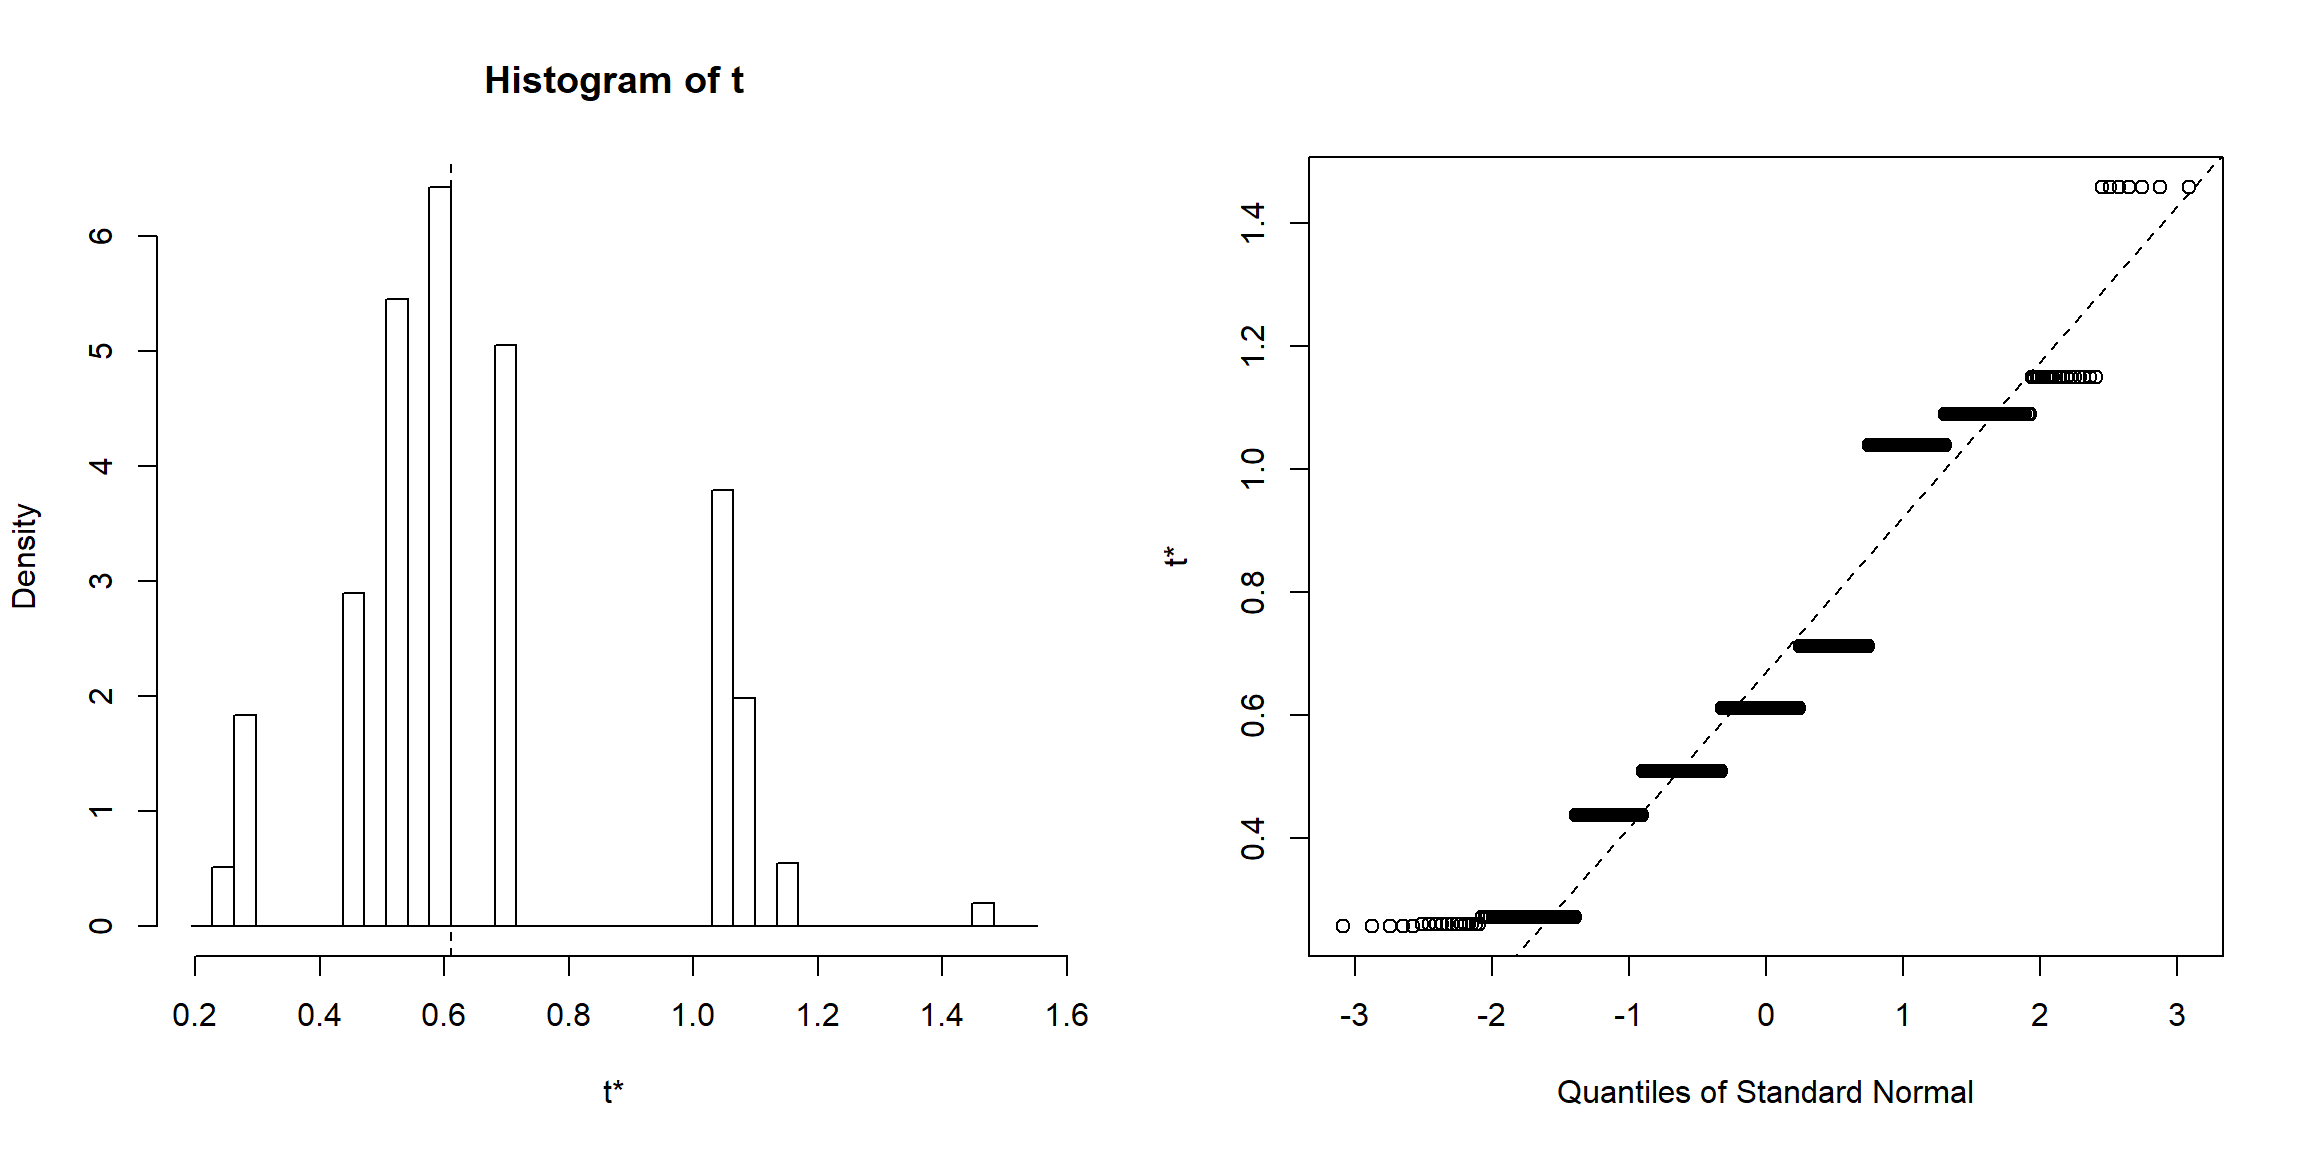
\includegraphics[width=0.7\linewidth]{01-intro_files/figure-latex/plot-res-boot-1} 

}

\caption{Gráficos de diagnóstico de los resultados bootstrap de la mediana de los tiempos de vida de microorganismos.}\label{fig:plot-res-boot}
\end{figure}

Además de estos métodos, las principales funciones de interés serían:

\begin{itemize}
\item
  \texttt{jack.after.boot()}: genera un gráfico para diagnósticar la
  inluencia de las observaciones individuales en los resultados
  bootstrap (se representan los cuantiles frente a las diferencias en el
  estadístico al eliminar una observación; este gráfico también se puede
  obtener estableciendo \texttt{jack\ =\ TRUE} en \texttt{plot.boot()}).
\item
  \texttt{boot.array()}: genera la matriz de índices a partir de la que
  se obtuvieron las remuestras (permite reconstruir las remuestras
  bootstrap).
\item
  \texttt{boot.ci()}: construye distintos tipos de intervalos de
  confianza (se tratarán en el Capítulo \ref{cap5}) dependiendo del
  parámetro \texttt{type}:

  \begin{itemize}
  \item
    \texttt{"norm"}: utiliza la distribución asintótica normal
    considerando las aproximaciones bootstrap del sesgo y de la
    varianza.
  \item
    \texttt{"basic"}: emplea el estadístico \(R = \hat \theta - \theta\)
    para la construcción del intervalo de confianza.
  \item
    \texttt{"stud"}: calcula el intervalo a partir del estadístico
    estudentizado
    \(R = \left( \hat \theta - \theta \right) / \sqrt{Var(\hat \theta)}\).
  \item
    \texttt{"perc"}: utiliza directamente la distribución bootstrap del
    estadístico (\(R = \hat \theta\)).
  \item
    \texttt{"bca"}: emplea el método \(BCa\) (``bias-corrected and
    accelerated'') propuesto por Efron (1987) (ver Sección 5.3.2 de
    Davison y Hinkley, 1997).
  \item
    \texttt{"all"}: calcula los cinco tipos de intervalos anteriores.
  \end{itemize}
\end{itemize}

Como ya se comentó, la función \texttt{boot()} admite estadísticos
multivariantes (haciendo que la función \texttt{statistic} devuelva un
vector en lugar de un escalar), pero por defecto las funciones
anteriores consideran el primer componente como el estadístico
principal. Para obtener resultados de otros componentes del vector de
estadísticos habrá que establecer el parámetro \texttt{index} igual al
índice deseado. Además, en algunos casos (por ejemplo para la obtención
de intevalos de confianza estudentizados con la función
\texttt{boot.ci()}) se supone, por defecto, que el segundo componente
del vector de estadísticos contiene estimaciones de la varianza del
estadístico para cada réplica boostrap.

\BeginKnitrBlock{example}[Inferencia sobre la media con varianza desconocida, continuación]
\protect\hypertarget{exm:media-dt-desconocida-boot}{}{\label{exm:media-dt-desconocida-boot}
\iffalse (Inferencia sobre la media con varianza desconocida,
continuación) \fi{} } \vspace{0.5cm}

Continuando con el Ejemplo \ref{exm:media-dt-desconocida} de inferencia
sobre la media con varianza desconocida. Para obtener la estimación por
intervalo de confianza del tiempo de vida medio de los microorganismos
con el paquete \texttt{boot}, podríamos emplear el siguiente código:
\EndKnitrBlock{example}

\begin{Shaded}
\begin{Highlighting}[]
\KeywordTok{library}\NormalTok{(boot)}
\NormalTok{muestra <-}\StringTok{ }\KeywordTok{c}\NormalTok{(}\FloatTok{0.143}\NormalTok{, }\FloatTok{0.182}\NormalTok{, }\FloatTok{0.256}\NormalTok{, }\FloatTok{0.26}\NormalTok{, }\FloatTok{0.27}\NormalTok{, }\FloatTok{0.437}\NormalTok{, }\FloatTok{0.509}\NormalTok{, }
             \FloatTok{0.611}\NormalTok{, }\FloatTok{0.712}\NormalTok{, }\FloatTok{1.04}\NormalTok{, }\FloatTok{1.09}\NormalTok{, }\FloatTok{1.15}\NormalTok{, }\FloatTok{1.46}\NormalTok{, }\FloatTok{1.88}\NormalTok{, }\FloatTok{2.08}\NormalTok{)}

\NormalTok{statistic <-}\StringTok{ }\ControlFlowTok{function}\NormalTok{(data, i)\{}
\NormalTok{  remuestra <-}\StringTok{ }\NormalTok{data[i]}
  \KeywordTok{c}\NormalTok{(}\KeywordTok{mean}\NormalTok{(remuestra), }\KeywordTok{var}\NormalTok{(remuestra)}\OperatorTok{/}\KeywordTok{length}\NormalTok{(remuestra))}
\NormalTok{\}}

\KeywordTok{set.seed}\NormalTok{(}\DecValTok{1}\NormalTok{)}
\NormalTok{res.boot <-}\StringTok{ }\KeywordTok{boot}\NormalTok{(muestra, statistic, }\DataTypeTok{R =} \DecValTok{1000}\NormalTok{)}
\NormalTok{res.boot}
\end{Highlighting}
\end{Shaded}

\begin{verbatim}
## 
## ORDINARY NONPARAMETRIC BOOTSTRAP
## 
## 
## Call:
## boot(data = muestra, statistic = statistic, R = 1000)
## 
## 
## Bootstrap Statistics :
##      original       bias    std. error
## t1* 0.8053333  0.001745067 0.157310082
## t2* 0.0259338 -0.001404917 0.007962592
\end{verbatim}

\begin{Shaded}
\begin{Highlighting}[]
\KeywordTok{boot.ci}\NormalTok{(res.boot)}
\end{Highlighting}
\end{Shaded}

\begin{verbatim}
## BOOTSTRAP CONFIDENCE INTERVAL CALCULATIONS
## Based on 1000 bootstrap replicates
## 
## CALL : 
## boot.ci(boot.out = res.boot)
## 
## Intervals : 
## Level      Normal              Basic             Studentized     
## 95%   ( 0.4953,  1.1119 )   ( 0.4945,  1.1121 )   ( 0.5055,  1.2705 )  
## 
## Level     Percentile            BCa          
## 95%   ( 0.4986,  1.1161 )   ( 0.5289,  1.1285 )  
## Calculations and Intervals on Original Scale
\end{verbatim}

El intervalo marcado como \texttt{Studentized} se obtuvo empleando el
mismo estadístico del Ejemplo \ref{exm:media-dt-desconocida}.

\textbf{\emph{Modificaciones del bootstrap uniforme}}

Establecenciendo parámetros adicionales de la función \texttt{boot} se
pueden llevar a cabo modificaciones del bootstrap uniforme. Algunos de
estos parámetros son los siguientes:

\begin{itemize}
\item
  \texttt{strata}: permite realizar remuestreo estratificado
  estableciendo este parámetro como un vector numérico o factor que
  defina los grupos.
\item
  \texttt{sim\ =\ c("ordinary"\ ,\ "parametric",\ "balanced",\ "permutation",\ "antithetic")}:
  permite establecer distintos tipos de remuestreo. Por defecto es igual
  a \texttt{"ordinary"} que se corresponde con el bootstrap uniforme,
  descrito anteriormente. Entre el resto de opciones destacaríamos
  \texttt{sim\ =\ "permutation"}, que permite realizar contrastes de
  permutaciones (remuestreo sin reemplazamiento), y
  \texttt{sim\ =\ "parametric"}, que permite realizar bootstrap
  paramétrico (Sección \ref{cap4-boot-par}). En este último caso también
  habrá que establecer los parámetros \texttt{ran.gen} y \texttt{mle}, y
  la función \texttt{statistics} no empleará el segundo parámetro de
  índices.
\item
  \texttt{ran.gen}: función que genera los datos. El primer argumento
  será el conjunto de datos original y el segundo un vector de
  parámetros adicionales (normalmente los valores de los parámetros de
  la distribución).
\item
  \texttt{mle}: parámetros de la distribución (típicamente estimados por
  máxima verosimilitud) o parámetros adicionales para \texttt{ran.gen} ó
  \texttt{statistics}.
\end{itemize}

Además hay otros parámetros para el procesamiento en paralelo:
\texttt{parallel\ =\ c("no",\ "multicore",\ "snow")}, \texttt{ncpus},
\texttt{cl}. Para más detalles sobre los parámetros consultar la ayuda
de la función \texttt{boot()} (\texttt{?boot}).

El paquete \texttt{boot} también incluye otras funciones que implementan
métodos boostrap para otros tipos de datos, como la función
\texttt{censboot()} para datos censurados (Capítulo \ref{cap8}) o la
función \texttt{tsboot()} para series de tiempo (Capítulo \ref{cap9}).

\chapter{Estimación de la precisión y el sesgo de un
estimador}\label{cap2}

Uno de los problemas más interesantes que pueden ser abordados desde la
perspectiva de los métodos de remuestreo es el de la estimación del
sesgo y la precisión de un estimador. En dicho contexto surgió el método
Jackknife (bastante antes que el bootstrap), que, en ese sentido, puede
considerarse el método de remuestreo más antiguo como tal.

\section{Estimación bootstrap de la precisión y el sesgo de un
estimador}\label{cap2-boot}

Consideremos \(\mathbf{X}=\left( X_1,\ldots ,X_n \right)\) una m.a.s. de
una población con distribución \(F\) y supongamos que tenemos interés en
realizar inferencia sobre un parámetro de la población
\(\theta =\theta \left( F \right)\). Consideremos un estimador,
\(\hat{\theta}=T\left( \mathbf{X} \right)\), de dicho parámetro y
definamos el estadístico
\[R=R\left( \mathbf{X}, F \right) = T\left( \mathbf{X} \right) 
- \theta \left( F \right) = \hat{\theta} - \theta.\] El sesgo del
estimador no es más que la esperanza del estadístico \(R\) y la varianza
de \(\hat{\theta}\) es también la varianza de \(R\) (pues \(\theta\) no
es aleatorio). Además, el error cuadrático medio del estimador también
se puede escribir como el momento de orden 2 de \(R\): \[\begin{aligned}
Sesgo\left( \hat{\theta} \right) &= E\left( \hat{\theta}-\theta \right)
=E\left( R \right), \\
Var\left( \hat{\theta} \right) &= Var\left( \hat{\theta}-\theta \right)
=Var\left( R \right), \\
MSE\left( \hat{\theta} \right) &= E\left[ \left( \hat{\theta}-\theta \right)
^2\right] =E\left( R^2 \right).
\end{aligned}\]

Dado que el principio bootstrap es útil para aproximar la distribución
en muestreo del estadístico \(R\), entonces también permitirá aproximar
sus momentos (su esperanza, su varianza, la esperanza de su cuadrado) y
así proceder según sigue:

\begin{enumerate}
\def\labelenumi{\arabic{enumi}.}
\item
  Estimar la función de distribución de probabilidad mediante
  \(\hat{F}\)
\item
  Para cada \(i=1,\ldots ,n\) arrojar \(X_i^{\ast}\) a partir de
  \(\hat{F}\) y obtener
  \(\mathbf{X}^{\ast}=\left( X_1^{\ast}, \ldots ,X_n^{\ast} \right)\)
\item
  Calcular
  \(R^{\ast}=R\left( \mathbf{X}^{\ast},\hat{F} \right) =T\left( \mathbf{X}^{\ast} \right) -\theta \left( \hat{F} \right) = \hat{\theta}^{\ast}- \hat \theta\)
\item
  Repetir \(B\) veces los pasos 2-3 para obtener las réplicas bootstrap
  \(R^{\ast (1)}, \ldots, R^{\ast (B)}\)
\item
  Calcular el estimador bootstrap del sesgo:
  \[Sesgo^{\ast}\left( \hat{\theta}^{\ast} \right) =\bar{R}^{\ast}=\frac{1
  }{B}\sum_{b=1}^{B}R^{\ast (b)}.\]
\end{enumerate}

El algoritmo anterior es útil para aproximar por bootstrap el sesgo. Si
se desea aproximar la varianza puede sustituirse al paso 5 por:

\begin{enumerate}
\def\labelenumi{\arabic{enumi}.}
\setcounter{enumi}{4}
\tightlist
\item
  Calcular el estimador bootstrap de la varianza:
  \[Var^{\ast}\left( \hat{\theta}^{\ast} \right) =\frac{1}{B}
  \sum_{b=1}^{B}\left( R^{\ast (b)}-\bar{R}^{\ast} \right)^2\]
\end{enumerate}

Si se trata de aproximar por bootstrap el error cuadrático medio, el
paso 5 pasaría a ser:

\begin{enumerate}
\def\labelenumi{\arabic{enumi}.}
\setcounter{enumi}{4}
\tightlist
\item
  Calcular el estimador bootstrap del error cuadrático medio:
  \(MSE^{\ast}\left( \hat{\theta}^{\ast} \right) =\frac{1}{B}\sum_{b=1}^{B}R^{\ast (b) 2}\)
\end{enumerate}

En el caso de la varianza podría ahorrarse algunos cálculos definiendo
directamente \(R=T\left( \mathbf{X} \right) =\hat{\theta}\) y,
consecuentemente,
\(R^{\ast}=T\left( \mathbf{X}^{\ast} \right) = \hat{\theta}^{\ast}\).
Así otro algoritmo de cálculo algo menos intensivo sería:

\begin{enumerate}
\def\labelenumi{\arabic{enumi}.}
\item
  Estimar la función de distribución de probabilidad mediante
  \(\hat{ F}\)
\item
  Para cada \(i=1,\ldots ,n\) arrojar \(X_i^{\ast}\) a partir de
  \(\hat{F}\) y obtener
  \(\mathbf{X}^{\ast}=\left( X_1^{\ast}, \ldots, X_n^{\ast} \right)\)
\item
  Calcular \(T\left( \mathbf{X}^{\ast} \right) = \hat{\theta}^{\ast}\)
\item
  Repetir \(B\) veces los pasos 2-3 para obtener las réplicas bootstrap
  \(\hat{\theta}^{\ast (1)}, \ldots, \hat{\theta}^{\ast(B)}\)
\item
  Calcular
  \(\overline{\hat{\theta}^{\ast}}=\frac{1}{B}\sum_{b=1}^{B}\hat{ \theta}^{\ast (b)}\)
  y, con ello,
  \(Var^{\ast}\left( \hat{\theta}^{\ast} \right) =\frac{1}{B}\sum_{b=1}^{B}\left( \hat{\theta}^{\ast \left(b \right)}-\overline{\hat{\theta}^{\ast}} \right)^2\)
\end{enumerate}

Es interesante mencionar que esto permite aproximar por bootstrap
(mediante Monte Carlo) la varianza de un estimador sin conocer una
expresión explícita para dicha varianza teórica. En general, el
estimador, \(\hat{F}\), de \(F\) a utilizar en los pasos 1-2 de estos
algoritmos se elije según proceda al caso. En el caso del bootstrap
uniforme sería \(\hat{F}=F_n\) y se puede proceder como se mostró en la
Sección \ref{cap1-implementacion}.

\subsection{Ejemplo: la media muestral}\label{ejemplo-la-media-muestral}

Consideremos como parámetro de interés la media de la población,
\(\theta =\theta \left( F \right) =\mu =\int xdF\left( x \right)\), y
tomemos como estimador la media muestral:
\(\hat{\theta}=\hat{\mu}=T\left( \mathbf{X} \right) =\bar{X}=\frac{1}{n}\sum_{j=1}^{n}X_j\).
Supongamos que deseamos estudiar la varianza de este estimador:
\(Var\left( \hat{\theta} \right) =Var\left( \bar{X} \right) =\frac{\sigma^2}{n}\).

A la hora de aproximar por bootstrap \(Var\left( \hat{\theta} \right)\),
si no disponemos de ninguna otra información adicional (como que la
distribución sea de cierta familia paramétrica o que sea continua),
parece razonable elegir como método de remuestreo el bootstrap uniforme.
En tal caso el algoritmo bootstrap de Monte Carlo procedería de esta
forma:

\begin{enumerate}
\def\labelenumi{\arabic{enumi}.}
\item
  Para cada \(i=1,\ldots ,n\) arrojar
  \(U_i\sim \mathcal{U}\left( 0,1 \right)\) y hacer
  \(X_i^{\ast}=X_{\left\lfloor nU_i\right\rfloor +1}\)
\item
  Calcular
  \(T\left( \mathbf{X}^{\ast} \right) =\bar{X}^{\ast}= \frac{1}{n}\sum_{i=1}^{n}X_i^{\ast}\)
\item
  Repetir \(B\) veces los pasos 1-2 para obtener las réplicas bootstrap
  \(\bar{X}^{\ast (1)}, \ldots, \bar{X}^{\ast (B)}\)
\item
  Calcular \(\overline{\bar{X}^{\ast}}=\frac{1}{B}\sum_{b=1}^{B}\)
  \(\bar{X}^{\ast (b)}\) y
  \(Var^{\ast}\left( \bar{X}^{\ast} \right) =\frac{1}{B} \sum_{b=1}^{B}\left( \bar{X}^{\ast (b)}-\overline{\bar{X}^{\ast}} \right)^2\)
\end{enumerate}

De todas formas, en este caso puede verse fácilmente que no es necesario
realizar Monte Carlo. En efecto, \[\begin{aligned}
Var^{\ast}\left( \bar{X}^{\ast} \right) & = \frac{1}{n^2}
\sum_{i=1}^{n}Var^{\ast}\left( X_i^{\ast} \right) =\frac{1}{n}Var^{\ast}\left( X_1^{\ast} \right) \\
& = \frac{1}{n}\left\{ E^{\ast}\left( X_1^{\ast 2} \right) -
\left[ E^{\ast}\left( X_1^{\ast} \right) \right]^2\right\} =\frac{1}{n}\left[ 
\frac{1}{n}\sum_{j=1}^{n}X_j^2-\left( \frac{1}{n}\sum_{j=1}^{n}X_j \right)^2 \right] \\
& = \frac{1}{n^2}\sum_{j=1}^{n}\left( X_j-\bar{X} \right)^2=\frac{S_n^2}{n},
\end{aligned}\] que es precisamente el estimador plug-in de la varianza
de la media muestral.

\BeginKnitrBlock{example}[Aproximación bootstrap de la precisión de estimaciones del tiempo de vida medio de microorganismos]
\protect\hypertarget{exm:estimacion-boot-precision}{}{\label{exm:estimacion-boot-precision}
\iffalse (Aproximación bootstrap de la precisión de estimaciones del
tiempo de vida medio de microorganismos) \fi{} } \vspace{0.5cm}

Continuando con el ejemplo de los tiempos de vida de microorganismos,
supongamos que queremos estimar la precisión de dos estimadores de su
vida media: media muestral y mediana muestral, a partir de los datos
observados: 0.143, 0.182, 0.256, 0.260, 0.270, 0.437, 0.509, 0.611,
0.712, 1.04, 1.09, 1.15, 1.46, 1.88, 2.08.
\EndKnitrBlock{example}

La estimación media muestral resulta \(\bar{X}=0.8053333\). Por su parte
la estimación mediana muestral es \(x_{\left( 8 \right)}=0.611\).

La varianza del estimador media muestral, \(\bar{X}\) es
\(Var\left( \bar{X} \right) =\frac{\sigma^2}{n}\), desconocida en este
caso. Su estimación bootstrap (idéntica a la plug-in) mediante un
remuestreo uniforme es calculable sin necesidad de realizar Monte Carlo
y resulta: \[Var^{\ast}\left( \bar{X}^{\ast} \right) =\frac{1}{n^2}
\sum_{j=1}^{n}\left( x_j-\bar{X} \right)^2=0.024204877.\] Con lo cual
\(\sqrt{Var^{\ast}\left( \bar{X}^{\ast} \right)}=\sqrt{ 0.024204877}= 0.155\,58\)

Si consideramos ahora la mediana muestral (como estimador de la media),
también sabemos que su distribución bootstrap puede calcularse de forma
explícita, sin necesidad de realizar Monte Carlo. Su masa de
probabilidad viene dada por:

\[\begin{aligned}
P^{\ast}\left( X_{\left( 8 \right)}^{\ast}=x_{(1)} \right)
&= 1-\sum_{k=0}^{m-1}\binom{n}{k}\left( \frac{1}{n} \right)^{k}\left( \frac{
n-1}{n} \right)^{n-k} \\
P^{\ast}\left( X_{\left( 8 \right)}^{\ast}=x_{(j)} \right)
&= \sum_{k=0}^{m-1}\binom{n}{k}\left[ \left( \frac{j-1}{n} \right)^{k}\left( 
\frac{n-j+1}{n} \right)^{n-k} - \left( \frac{j}{n} \right)^{k}\left( \frac{n-j}{n} \right)^{n-k}
\right] \\
\text{para }j &= 2,\ldots ,n
\end{aligned}\]

Con los datos concretos del ejemplo resulta: \[\begin{array}{ll}
P^{\ast}\left( X_{\left( 8 \right)}^{\ast} = 0.143 \right) = 1.639\times 10^{-6}\text{, } 
& P^{\ast}\left( X_{\left( 8 \right)}^{\ast} = 0.182 \right) = 2.655\times 10^{-4},\\
P^{\ast}\left( X_{\left( 8 \right)}^{\ast} = 0.256 \right) = 3.973\times 10^{-3}\text{, } 
& P^{\ast}\left( X_{\left( 8 \right)}^{\ast} = 0.260 \right) = 2.121\times 10^{-2}, \\
P^{\ast}\left( X_{\left( 8 \right)}^{\ast} = 0.270 \right) = 6.278\times 10^{-2}\text{, }
& P^{\ast}\left( X_{\left( 8 \right)}^{\ast} = 0.437 \right) = 0.1249, \\
P^{\ast}\left( X_{\left( 8 \right)}^{\ast} = 0.509 \right) = 0.1832\text{, }
& P^{\ast}\left( X_{\left( 8 \right)}^{\ast} = 0.611 \right) = 0.2073,\\
P^{\ast}\left( X_{\left( 8 \right)}^{\ast} = 0.712 \right) = 0.1832\text{, }
& P^{\ast}\left( X_{\left( 8 \right)}^{\ast} = 1.04 \right) = 0.1249,\\
P^{\ast}\left( X_{\left( 8 \right)}^{\ast} = 1.09 \right) = 6.278\times 10^{-2}\text{, }
& P^{\ast}\left( X_{\left( 8 \right)}^{\ast} = 1.15 \right) = 2.121\times 10^{-2}, \\
P^{\ast}\left( X_{\left( 8 \right)}^{\ast} = 1.46 \right) = 3.973\times 10^{-3}\text{, }
& P^{\ast}\left( X_{\left( 8 \right)}^{\ast} = 1.88 \right) = 2.655\times 10^{-4}, \\
P^{\ast}\left( X_{\left( 8 \right)}^{\ast} = 2.08 \right) = 1.639\times 10^{-6}. 
\end{array}\]

Como consecuencia, \[\begin{aligned}
E^{\ast}\left( X_{\left( 8 \right)}^{\ast} \right)
&= \sum_{j=1}^{15}x_{(j)}P^{\ast}\left( X_{\left( 8 \right)
}^{\ast}=x_{(j)} \right) =0.65749924 \\
E^{\ast}\left( X_{\left( 8 \right)}^{\ast 2} \right)
&= \sum_{j=1}^{15}x_{(j)}^2P^{\ast}\left( X_{\left( 8 \right)
}^{\ast}=x_{(j)} \right) =0.49500381 \\
Var^{\ast}\left( X_{\left( 8 \right)}^{\ast} \right)
&= 0.49500381-0.65749924^2=6.\, 2699\times 10^{-2} \\
\sqrt{Var^{\ast}\left( X_{\left( 8 \right)}^{\ast} \right)} &= \sqrt{
6.\, 2699\times 10^{-2}}=0.250\,40
\end{aligned}\]

Las estimaciones bootstrap de los errores cuadráticos medios de ambos
estimadores (como estimadores de la media poblacional) son:
\[\begin{aligned}
MSE^{\ast}\left( \bar{X}^{\ast} \right) &= \left( E^{\ast}\left( 
\bar{X}^{\ast} \right) -\bar{X} \right)^2+Var^{\ast}\left( 
\bar{X}^{\ast} \right) \\
&= Var^{\ast}\left( \bar{X}^{\ast} \right) =0.024204877, \\
MSE^{\ast}\left( X_{\left( 8 \right)}^{\ast} \right) &= \left( E^{\ast
}\left( X_{\left( 8 \right)}^{\ast} \right) -\bar{X} \right)
^2+Var^{\ast}\left( X_{\left( 8 \right)}^{\ast} \right) = \\
&= \left( 0.65749924-0.8053333 \right)^2+6.2699 \times 10^{-2}\\
&=  0.084554.
\end{aligned}\]

Una aproximación de Monte Carlo de estas varianzas bootstrap se puede
llevar a cabo mediante el siguiente código:

\begin{Shaded}
\begin{Highlighting}[]
\CommentTok{# Para la muestra de TIEMPOS DE VIDA, estima (plug-in) la precisión }
\CommentTok{# de la media muestral (desvmedia) y también aproxima por Monte Carlo}
\CommentTok{# la estimación bootstrap de dicha precisión (desvmediaboot) y}
\CommentTok{# también la precisión de la mediana muestral, de la cual no se}
\CommentTok{# conoce su expresión, (desvmedianaboot).}
\CommentTok{# También estima el sesgo bootstrap de esos dos estimadores }
\CommentTok{# (sesgomediaboot y sesgomedianaboot, respectivamente).}

\NormalTok{muestra <-}\StringTok{ }\KeywordTok{c}\NormalTok{(}\FloatTok{0.143}\NormalTok{, }\FloatTok{0.182}\NormalTok{, }\FloatTok{0.256}\NormalTok{, }\FloatTok{0.26}\NormalTok{, }\FloatTok{0.27}\NormalTok{, }\FloatTok{0.437}\NormalTok{, }\FloatTok{0.509}\NormalTok{,}
    \FloatTok{0.611}\NormalTok{, }\FloatTok{0.712}\NormalTok{, }\FloatTok{1.04}\NormalTok{, }\FloatTok{1.09}\NormalTok{, }\FloatTok{1.15}\NormalTok{, }\FloatTok{1.46}\NormalTok{, }\FloatTok{1.88}\NormalTok{, }\FloatTok{2.08}\NormalTok{)}
\NormalTok{n <-}\StringTok{ }\KeywordTok{length}\NormalTok{(muestra)}
\NormalTok{varmedia <-}\StringTok{ }\NormalTok{(}\DecValTok{1}\OperatorTok{/}\NormalTok{(n}\OperatorTok{^}\DecValTok{2}\NormalTok{)) }\OperatorTok{*}\StringTok{ }\KeywordTok{sum}\NormalTok{((muestra }\OperatorTok{-}\StringTok{ }\KeywordTok{mean}\NormalTok{(muestra))}\OperatorTok{^}\DecValTok{2}\NormalTok{)}
\CommentTok{# Alternativamente: varmedia <- var(muestra)/n}
\NormalTok{desvmedia <-}\StringTok{ }\KeywordTok{sqrt}\NormalTok{(varmedia)}

\CommentTok{# Remuestreo}
\NormalTok{B <-}\StringTok{ }\FloatTok{1e+04}
\NormalTok{media <-}\StringTok{ }\KeywordTok{numeric}\NormalTok{(B)}
\NormalTok{mediana <-}\StringTok{ }\KeywordTok{numeric}\NormalTok{(B)}
\ControlFlowTok{for}\NormalTok{ (k }\ControlFlowTok{in} \DecValTok{1}\OperatorTok{:}\NormalTok{B) \{}
\NormalTok{    remuestra <-}\StringTok{ }\KeywordTok{sample}\NormalTok{(muestra, n, }\DataTypeTok{replace =} \OtherTok{TRUE}\NormalTok{)}
\NormalTok{    media[k] <-}\StringTok{ }\KeywordTok{mean}\NormalTok{(remuestra)}
    \CommentTok{# remordenada <- sort(remuestra)}
    \CommentTok{# mediana[k] <- remordenada[8]}
\NormalTok{    mediana[k] <-}\StringTok{ }\KeywordTok{median}\NormalTok{(remuestra)}
\NormalTok{\}}

\CommentTok{# Aproximaciones precisión}
\NormalTok{varmediaboot <-}\StringTok{ }\NormalTok{(}\DecValTok{1}\OperatorTok{/}\NormalTok{B) }\OperatorTok{*}\StringTok{ }\KeywordTok{sum}\NormalTok{((media }\OperatorTok{-}\StringTok{ }\KeywordTok{mean}\NormalTok{(media))}\OperatorTok{^}\DecValTok{2}\NormalTok{)}
\NormalTok{desvmediaboot <-}\StringTok{ }\KeywordTok{sqrt}\NormalTok{(varmediaboot)}
\NormalTok{varmedianaboot <-}\StringTok{ }\NormalTok{(}\DecValTok{1}\OperatorTok{/}\NormalTok{B) }\OperatorTok{*}\StringTok{ }\KeywordTok{sum}\NormalTok{((mediana }\OperatorTok{-}\StringTok{ }\KeywordTok{mean}\NormalTok{(mediana))}\OperatorTok{^}\DecValTok{2}\NormalTok{)}
\NormalTok{desvmedianaboot <-}\StringTok{ }\KeywordTok{sqrt}\NormalTok{(varmedianaboot)}
\NormalTok{desvmedia}
\end{Highlighting}
\end{Shaded}

\begin{verbatim}
## [1] 0.1555792
\end{verbatim}

\begin{Shaded}
\begin{Highlighting}[]
\NormalTok{desvmediaboot}
\end{Highlighting}
\end{Shaded}

\begin{verbatim}
## [1] 0.1552919
\end{verbatim}

\begin{Shaded}
\begin{Highlighting}[]
\NormalTok{desvmedianaboot}
\end{Highlighting}
\end{Shaded}

\begin{verbatim}
## [1] 0.2497064
\end{verbatim}

\begin{Shaded}
\begin{Highlighting}[]
\CommentTok{# Aproximaciones sesgo}
\NormalTok{sesgomediaboot <-}\StringTok{ }\KeywordTok{mean}\NormalTok{(media) }\OperatorTok{-}\StringTok{ }\KeywordTok{mean}\NormalTok{(muestra)}
\NormalTok{sesgomedianaboot <-}\StringTok{ }\KeywordTok{mean}\NormalTok{(mediana) }\OperatorTok{-}\StringTok{ }\NormalTok{muestra[}\DecValTok{8}\NormalTok{]}
\NormalTok{sesgomediaboot}
\end{Highlighting}
\end{Shaded}

\begin{verbatim}
## [1] -0.00056106
\end{verbatim}

\begin{Shaded}
\begin{Highlighting}[]
\NormalTok{sesgomedianaboot}
\end{Highlighting}
\end{Shaded}

\begin{verbatim}
## [1] 0.0462533
\end{verbatim}

Empleando el paquete \texttt{boot} el código sería más simple:

\begin{Shaded}
\begin{Highlighting}[]
\KeywordTok{library}\NormalTok{(boot)}
\NormalTok{statistic <-}\StringTok{ }\ControlFlowTok{function}\NormalTok{(data, i)\{}
\NormalTok{  remuestra <-}\StringTok{ }\NormalTok{data[i]}
  \KeywordTok{c}\NormalTok{(}\KeywordTok{mean}\NormalTok{(remuestra), }\KeywordTok{median}\NormalTok{(remuestra))}
\NormalTok{\}}

\KeywordTok{set.seed}\NormalTok{(}\DecValTok{1}\NormalTok{)}
\NormalTok{res.boot <-}\StringTok{ }\KeywordTok{boot}\NormalTok{(muestra, statistic, }\DataTypeTok{R =}\NormalTok{ B)}
\NormalTok{res.boot}
\end{Highlighting}
\end{Shaded}

\begin{verbatim}
## 
## ORDINARY NONPARAMETRIC BOOTSTRAP
## 
## 
## Call:
## boot(data = muestra, statistic = statistic, R = B)
## 
## 
## Bootstrap Statistics :
##      original      bias    std. error
## t1* 0.8053333 -0.00046904   0.1550047
## t2* 0.6110000  0.04636960   0.2498358
\end{verbatim}

Lamentablemente la función \texttt{print.boot()} calcula las
aproximaciones bootstrap del sesgo y de la precisión pero no las
almacena. En el caso más simple podríamos obtenerlas con el siguiente
código:

\begin{Shaded}
\begin{Highlighting}[]
\NormalTok{op <-}\StringTok{ }\KeywordTok{with}\NormalTok{(res.boot, }\KeywordTok{cbind}\NormalTok{(}
\NormalTok{  t0, }\KeywordTok{apply}\NormalTok{(t, }\DecValTok{2}\NormalTok{, mean, }\DataTypeTok{na.rm =} \OtherTok{TRUE}\NormalTok{) }\OperatorTok{-}\StringTok{  }\NormalTok{t0,}
  \KeywordTok{apply}\NormalTok{(t, }\DecValTok{2}\NormalTok{, sd, }\DataTypeTok{na.rm =} \OtherTok{TRUE}\NormalTok{)}
\NormalTok{  ))}
\KeywordTok{rownames}\NormalTok{(op) <-}\StringTok{ }\KeywordTok{paste0}\NormalTok{(}\StringTok{"t"}\NormalTok{, }\DecValTok{1}\OperatorTok{:}\KeywordTok{ncol}\NormalTok{(res.boot}\OperatorTok{$}\NormalTok{t), }\StringTok{"*"}\NormalTok{)}
\KeywordTok{colnames}\NormalTok{(op) <-}\StringTok{ }\KeywordTok{c}\NormalTok{(}\StringTok{"original"}\NormalTok{, }\StringTok{"bias  "}\NormalTok{, }\StringTok{" std. error"}\NormalTok{)}
\NormalTok{op}
\end{Highlighting}
\end{Shaded}

\begin{verbatim}
##      original      bias    std. error
## t1* 0.8053333 -0.00046904   0.1550047
## t2* 0.6110000  0.04636960   0.2498358
\end{verbatim}

\chapter{Motivación del método Jackknife}\label{cap3}

El jackknife es probablemente el método de remuestreo, propiamente
dicho, más antiguo. Fue propuesto por Quenouille (1949) para estimar el
sesgo de un estimador. Tukey (1958) bautiza el método y lo utiliza para
estimar la varianza de un estimador. En realidad el jackknife no suele
utilizarse para aproximar la distribución de
\(R\left( \mathbf{X},F \right)\), sino más bien para estimar
características de dicha variable aleatoria, como su esperanza o su
varianza.

La diferencia entre el bootstrap y el jackknife es muy fácil de expresar
en términos de los vectores de remuestreo. Así, el bootstrap uniforme
utiliza vectores de remuestreo de la forma
\(\mathbf{P}^{\ast}=\left( \frac{m_1}{n},\ldots ,\frac{m_n}{n} \right)\),
con \(m_i\in \mathbb{Z}^{+}\), \(i=1,\ldots ,n\), mientras que el
jackknife considera vectores de remuestreo de la forma
\[\mathbf{P}_{(i)}^{\ast}=\left( \frac{1}{n-1},\ldots ,\underset{(i)}{0}
,\ldots ,\frac{1}{n-1} \right).\] En otras palabras todas las remuestras
jackknife posibles son tantas como el tamaño muestral y cada una
consiste en eliminar una observación de la muestra, quedándose con una
remuestra de tamaño \(n-1\) en la que las demás observaciones aparecen
exactamente con frecuencia \(1\).

Evidentemente, el número de posibles remuestras jackknife, \(n\), es
muchísimo más pequeño que el número de remuestras bootstrap,
\(\binom{2n-1}{n}\), lo cual permite calcular con rapidez las
realizaciones del estadístico de interés en todas las posibles
remuestras jackknife.

\section{Estimación Jackknife de la precisión y el sesgo de un
estimador}\label{estimacion-jackknife-de-la-precision-y-el-sesgo-de-un-estimador}

Cuando estamos interesados en el sesgo o la varianza de un estimador
\(\hat{\theta}=\theta \left( \mathbf{X} \right)\) de un parámetro
\(\theta =\theta \left( F \right)\), el estadístico de interés suele
definirse como \(R=R\left( \mathbf{X},F \right) =\hat{\theta}-\theta\).
En este caso \[\begin{aligned}
Sesgo\left( \hat{\theta} \right) &= E\left( \hat{\theta} \right) -\theta
=E\left( R \right), \\
Var\left( \hat{\theta} \right) &= Var\left( \hat{\theta}-\theta \right)
=Var\left( R \right).
\end{aligned}\] Así pues trataremos de usar el jackknife para aproximar
la esperanza y varianza de \(R\), o, equivalentemente, el sesgo y la
varianza de \(\hat{\theta}\).

El conjunto de remuestras jackknife es
\[\mathcal{X}_{jackk}=\left\{ \mathbf{X}^{\ast}=
\mathbf{X}_{(i)}=\left( X_1,\ldots ,X_{i-1},X_{i+1},\ldots
,X_n \right) : i=1,\ldots ,n\right\}\] y todas ellas se consideran con
equiprobabilidad en el universo jackknife. Como primera tentativa
estimaríamos el sesgo y la varianza jackknife mediante:
\[\begin{aligned}
E^{\ast}\left( R^{\ast} \right) &= E_{jackk}^{\ast}\left( \hat{\theta}
^{\ast} \right) -\theta \left( \mathbf{X} \right) =\frac{1}{n}
\sum_{i=1}^{n}\theta \left( \mathbf{X}_{(i)} \right) -
\hat{\theta}=\overline{\theta \left( \mathbf{X}_{(\cdot)} \right)}-\hat{\theta}, \\
Var^{\ast}\left( R^{\ast} \right) &= Var_{jackk}^{\ast}\left( \hat{\theta}
^{\ast} \right) =\frac{1}{n}\sum_{i=1}^{n}\left[ \theta \left( 
\mathbf{X}_{(i)} \right) -\overline{\theta \left( 
\mathbf{X}_{(\cdot)} \right)}\right]^2,
\end{aligned}\] con
\(\overline{\theta \left( \mathbf{X}_{(\cdot)} \right)} = \frac{1}{n}\sum_{j=1}^{n}\theta \left( \mathbf{X}_{(j)} \right)\).

Sin embargo es evidente que las réplicas jackknife son mucho más
parecidas a la muestra original de lo que lo son las remuestras
bootstrap, en general. De hecho se puede demostrar que el valor absoluto
de ese estimador jackknife del sesgo es siempre menor que el valor
absoluto del sesgo bootstrap y que la estimación jackknife de la
varianza que se acaba de proponer también es menor que la varianza
bootstrap. En resumen, el método jackknife necesita de un \textbf{factor
de elevación} para que las estimaciones que proporciona sean
consistentes. La idea es elegir dicho factor de elevación como aquel que
provoca que, al multiplicar los estadísticos anteriores por él, y
considerando como parámetro a estimar la media o la varianza
poblacional, el estimador jackknife finalmente resultante sea insesgado.
Así, el factor de elevación resulta ser \(n-1\) y las estimaciones
jackknife finales son

\[\begin{aligned}
Sesgo_{jackk}^{\ast}\left( \hat{\theta}^{\ast} \right) &= \left( n-1 \right)
\left( \overline{\theta \left( \mathbf{X}_{(\cdot)}
 \right)}-\hat{\theta} \right) =\frac{n-1}{n}\sum_{i=1}^{n}\left( \theta
\left( \mathbf{X}_{(i)} \right) -\hat{\theta} \right), \\
Var_{jackk}^{\ast}\left( \hat{\theta}^{\ast} \right) &= \frac{n-1}{n}
\sum_{i=1}^{n}\left[ \theta \left( \mathbf{X}_{(i)}
 \right) -\overline{\theta \left( \mathbf{X}_{(\cdot)}
 \right)}\right]^2.
\end{aligned}\]

Tomando como parámetro de interés la media, \(\theta =\mu\), tenemos que
\[\begin{aligned}
\overline{\theta \left( \mathbf{X}_{(\cdot)} \right)}-
\hat{\theta} &= \frac{1}{n}\sum_{i=1}^{n}\theta \left( 
\mathbf{X}_{(i)} \right) -\hat{\theta}=\frac{1}{n}\sum_{i=1}^{n}
\overline{X_{(i)}}-\bar{X}= \\
&= \frac{1}{n}\sum_{i=1}^{n}\frac{1}{n-1}\sum_{j=1,j\neq i}^{n}X_j-
\bar{X}=\frac{1}{n\left( n-1 \right)}\sum_{i,j=1,i\neq j}^{n}X_j-
\bar{X} \\
&= \frac{1}{n\left( n-1 \right)}\sum_{j=1}^{n}\left( n-1 \right) X_j-
\bar{X}=\frac{1}{n}\sum_{j=1}^{n}X_j-\bar{X}=0,\end{aligned}\]

así que
\(\overline{\theta \left( \mathbf{X}_{(\cdot)} \right)}-\hat{\theta}\)
es un estimador insesgado del sesgo de \(\bar{X}\) (que es cero). De
esta forma, utilizando un factor de elevación arbitrario, \(c\), se
tiene igualmente que
\[c\left( \overline{\theta \left( \mathbf{X}_{(\cdot)} \right)}
- \hat{\theta} \right) = 0,\] así que es también un estimador insesgado
de \(Sesgo\left( \bar{X} \right) =0.\)\$ Determinaremos el valor de
\(c\) imponiendo que el estimador jackknife de la varianza de dicho
estimador (\(\hat{\theta}=\bar{X}\)) es una estimador insesgado de la
varianza de dicho estimador. Por una parte, es bien conocido que la
varianza de \(\hat{\theta}\) es
\(Var\left( \bar{X} \right) = \sigma^2 /n\). Por otra parte, la
estimación jackknife de la varianza de \(\hat{\theta}\), con factor de
elevación \(c\) es

\[\begin{aligned}
Var_{jackk}^{\ast}\left( \bar{X} \right) &= \frac{c}{n}\sum_{i=1}^{n}
\left[ \overline{X_{(i)}}-\overline{\overline{X_{\left( \cdot
 \right)}}}\right]^2 \\
&= \frac{c}{n}\sum_{i=1}^{n}\left[ \frac{1}{n-1}\sum_{j=1,j\neq i}^{n}X_j-
\frac{1}{n}\sum_{k=1}^{n}\frac{1}{n-1}\sum_{j=1,j\neq k}^{n}X_j\right]^2
\\
&= \frac{c}{n}\sum_{i=1}^{n}\left[ \frac{1}{n-1}\sum_{j=1,j\neq i}^{n}X_j-
\frac{1}{n\left( n-1 \right)}\sum_{k,j=1,j\neq k}^{n}X_j\right]^2 \\
&= \frac{c}{n}\sum_{i=1}^{n}\left[ \frac{1}{n\left( n-1 \right)}
\sum_{j=1,j\neq i}^{n}X_j-\frac{1}{n}X_i\right]^2.\end{aligned}\]

La esperanza de esta cantidad resulta: \[\begin{aligned}
&E\left[ \frac{c}{n}\sum_{i=1}^{n}\left( \frac{1}{n\left( n-1 \right)}
\sum_{j=1,j\neq i}^{n}X_j-\frac{1}{n}X_i \right)^2\right] \\
&= \frac{c}{n}\sum_{i=1}^{n}E\left[ \left( \frac{1}{n\left( n-1 \right)}
\sum_{j=1,j\neq i}^{n}X_j-\frac{1}{n}X_i \right)^2\right] \\
&= \frac{c}{n}\sum_{i=1}^{n}E\left[ \left( \frac{1}{n\left( n-1 \right)}
\sum_{j=1,j\neq i}^{n}\left( X_j-\mu \right) 
-\frac{1}{n}\left( X_i-\mu \right) \right)^2\right] \\
&= \frac{c}{n}\sum_{i=1}^{n}Var\left[ \frac{1}{n\left( n-1 \right)}
\sum_{j=1,j\neq i}^{n}\left( X_j-\mu \right) 
-\frac{1}{n}\left( X_i-\mu \right) \right]\\
&= \frac{c}{n}\sum_{i=1}^{n}\left( \frac{1}{n^2\left( n-1 \right)^2}
\sum_{j=1,j\neq i}^{n}\sigma^2+\frac{1}{n^2}\sigma^2 \right) \\
&= \frac{c}{n}\sum_{i=1}^{n}\left( \frac{1}{n^2\left( n-1 \right)}\sigma^2+\frac{1}{n^2}\sigma^2 \right) 
=\frac{c\sigma^2}{n\left(n-1 \right)}.
\end{aligned}\]

Así pues, el sesgo del estimador jackknife de la varianza de la media
muestral es
\[E\left[ Var_{jackk}^{\ast}\left( \bar{X} \right) \right] -\frac{\sigma
^2}{n}=\frac{c\sigma^2}{n\left( n-1 \right)}-\frac{\sigma^2}{n}=
\frac{\sigma^2}{n}\left( \frac{c}{n-1}-1 \right),\] que vale cero si y
solamente si \(c=n-1\). Dicho en otras palabras, tomando como factor de
elevación \(c=n-1\), entonces, tanto el estimador jackknife del sesgo de
\(\bar{X}\) como el estimador jackknife de la varianza de \(\bar{X}\)
son estimadores insesgados, respectivamente, del sesgo y la varianza de
\(\bar{X}\).

Dichos estimadores resultan\[\begin{aligned}
Sesgo_{jackk}^{\ast}\left( \bar{X} \right) &= \left( n-1 \right) \left( 
\overline{\overline{X_{(\cdot)}}}-\bar{X} \right), \\
Var_{jackk}^{\ast}\left( \bar{X} \right) &= \frac{n-1}{n}\sum_{i=1}^{n}
\left[ \overline{X_{(i)}}-\overline{\overline{X_{\left( \cdot
 \right)}}}\right]^2.\end{aligned}\]

Podemos realizar un razonamiento análogo cuando el parámetro de interés
es la varianza poblacional, \(\theta =\sigma^2\). En ese caso,
considerando el estimador varianza muestral: \(\hat{\theta}=S_n^2\), se
tiene que su esperanza viene dada por

\[\begin{aligned}
E\left( S_n^2 \right) &= E\left[ \frac{1}{n}\sum_{i=1}^{n}\left( X_i-
\bar{X} \right)^2\right] =\frac{1}{n}\sum_{i=1}^{n}E\left[ \left(
X_i-\bar{X} \right)^2\right] \\
&= E\left[ \left( X_1-\frac{1}{n}\sum_{j=1}^{n}X_j \right)^2\right] =E
\left[ \left( \left( X_1-\mu \right) -\frac{1}{n}\sum_{j=1}^{n}\left(
X_j-\mu \right) \right)^2\right] \\
&= Var\left[ \left( X_1-\mu \right) -\frac{1}{n}\sum_{j=1}^{n}\left(
X_j-\mu \right) \right] \\
&= Var\left[ \frac{n-1}{n}\left( X_1-\mu \right) -\frac{1}{n}
\sum_{j=1,j\neq 1}^{n}\left( X_j-\mu \right) \right] \\
&= \left( \frac{n-1}{n} \right)^2\sigma^2+\frac{1}{n^2}
\sum_{j=2}^{n}\sigma^2 \\
&= \frac{\left( n-1 \right)}{n^2}^2\sigma^2+\frac{n-1}{n^2}\sigma
^2=\frac{n\left( n-1 \right)}{n^2}\sigma^2=\frac{n-1}{n}\sigma^2,\end{aligned}\]

así que su sesgo es
\[Sesgo\left( S_n^2 \right) =E\left( S_n^2 \right) -\sigma^2=-\frac{1
}{n}\sigma^2.\]Para un factor de elevación, \(c\), el estimador
jackknife del sesgo de este estimador
es\[Sesgo_{jackk}^{\ast}\left( S_n^2 \right) =c\left( \overline{\theta
\left( \mathbf{X}_{(\cdot)} \right)}-\hat{\theta}
 \right) =c\left( \overline{S_{n,(\cdot)}^2}-S_n^2 \right)
.\]Con lo cual la esperanza de este estimador resulta
\[E\left( c\left( \overline{S_{n,(\cdot)}^2}-S_n^2 \right)
 \right) =c\left[ E\left( \overline{S_{n,(\cdot)}^2} \right)
-E\left( S_n^2 \right) \right]\]

Estudiemos por separado cada término: \[\begin{aligned}
\overline{S_{n,(\cdot)}^2} &= \frac{1}{n}\sum_{i=1}^{n}S_{n,
(i)}^2=\frac{1}{n}\sum_{i=1}^{n}\frac{1}{n-1}\sum_{j=1,j\neq
i}^{n}\left( X_j-\overline{X_{(i)}} \right)^2 \\
&= \frac{1}{n}\sum_{i=1}^{n}\frac{1}{n-1}\sum_{j=1,j\neq i}^{n}\left( X_j-
\frac{1}{n-1}\sum_{k=1,k\neq i}^{n}X_{k} \right)^2 \\
&= \frac{1}{n\left( n-1 \right)}\sum_{i=1}^{n}\sum_{j=1,j\neq i}^{n}\left( 
\frac{n-2}{n-1}X_j-\frac{1}{n-1}\sum_{k=1,k\neq i,k\neq j}^{n}X_{k} \right)^2,
\end{aligned}\] con lo cual

\[\begin{aligned}
E\left( \overline{S_{n,(\cdot)}^2} \right) 
&=\frac{1}{n\left(
n-1 \right)}\sum_{i=1}^{n}\sum_{j=1,j\neq i}^{n}E\left[ \left( \frac{n-2}{n-1
}X_j-\frac{1}{n-1}\sum_{k=1,k\neq i,k\neq j}^{n}X_{k} \right)^2\right] \\
&=\frac{1}{n\left( n-1 \right)}\sum_{i=1}^{n}\sum_{j=1,j\neq i}^{n}E\left[
\left( \frac{n-2}{n-1}\left( X_j-\mu \right) -\frac{1}{n-1}\sum_{k=1,k\neq
i,k\neq j}^{n}\left( X_{k}-\mu \right) \right)^2\right] \\
&=\frac{1}{n\left( n-1 \right)}\sum_{i=1}^{n}\sum_{j=1,j\neq i}^{n}Var\left[ 
\frac{n-2}{n-1}\left( X_j-\mu \right) -\frac{1}{n-1}\sum_{k=1,k\neq
i,k\neq j}^{n}\left( X_{k}-\mu \right) \right] \\
&=\frac{1}{n\left( n-1 \right)}\sum_{i=1}^{n}\sum_{j=1,j\neq i}^{n}\left[ 
\frac{\left( n-2 \right)^2}{\left( n-1 \right)^2}\sigma^2+\frac{1}{
\left( n-1 \right)^2}\left( n-2 \right) \sigma^2\right] \\
&=\frac{1}{n\left( n-1 \right)}\sum_{i=1}^{n}\sum_{j=1,j\neq i}^{n}\left[ 
\frac{\left( n-2 \right) \left( n-1 \right)}{\left( n-1 \right)^2}\sigma
^2\right] =\frac{n-2}{n-1}\sigma^2
\end{aligned}\]

Además, ya hemos visto anteriormente que
\(E\left( S_n^2 \right) = (n-1)\sigma^2/n\), con o cual la esperanza del
estimador jackknife del sesgo es \[\begin{aligned}
c\left( \frac{n-2}{n-1}\sigma^2-\frac{n-1}{n}\sigma^2 \right)
&= c\sigma^2\left( \frac{n-2}{n-1}-\frac{n-1}{n} \right) \\
&= c\sigma^2\frac{n\left( n-2 \right) -\left( n-1 \right)^2}{n\left( n-1 \right)} \\
&= c\sigma^2\frac{-1}{n\left( n-1 \right)}
=-\frac{c\sigma^2}{n\left(n-1 \right)}.
\end{aligned}\]

De esta forma, el sesgo del estimador jackknife del sesgo de \(S_n^2\)
resulta ser \[\begin{aligned}
E\left[ Sesgo_{jackk}^{\ast}\left( S_n^2 \right) \right] 
-Sesgo\left(S_n^2 \right) &= -\frac{c\sigma^2}{n\left( n-1 \right)}
-\left( -\frac{1}{n}\sigma^2 \right) \\
&= -\frac{\sigma^2}{n}\left( \frac{c}{n-1}-1 \right),
\end{aligned}\]

con lo cual este sesgo será cero si y sólo si \(c=n-1\).

Esto da pie al estimador jackknife del sesgo de la varianza muestral:
\[Sesgo_{jackk}^{\ast}\left( S_n^2 \right) =\left( n-1 \right) \left( 
\overline{S_{n,(\cdot)}^2}-S_n^2 \right).\]

Así pues, queda justificado, en el caso de estimación de los parámetros
media y varianza, la razón de la elección del factor de elevación
\(c=n-1\).

\section{Relación Bootstrap/Jackknife en dicha
estimación}\label{relacion-bootstrapjackknife-en-dicha-estimacion}

Consideremos un parámetro de interés \(\theta \left( F \right)\) y su
correspondiente estimador que supondremos funcional,
\(\theta \left( F_n \right)\). En realidad, cuando calculamos cantidades
como \(\theta \left( \mathbf{X}_{(i)} \right)\), lo que estamos haciendo
es evaluar el funcional \(\theta\) en otra función de
distribución\[F_{n,(i)}\left( x \right) =\frac{1}{n-1}\sum_{j=1,j\neq i}^{n}
\mathbf{1}\left( X_j\leq x \right).\]Dicho en terminología de vectores
de remuestreo, el estimador habitual consiste en evaluar \(\theta\) en
el vector \(\mathbf{p}=\left( \frac{1}{n},\ldots ,\frac{1}{n} \right)\),
\(\theta \left( \mathbf{p} \right)\), mientras que el estimador
construido con toda la muestra excepto el dato \(i\)-ésimo es la
evaluación \(\theta \left( \mathbf{p}_{(i)} \right)\), siendo
\[\mathbf{p}_{(i)}=\left( \frac{1}{n-1},\ldots ,\frac{1}{n-1},
\underset{(i)}{0},\frac{1}{n-1},\ldots ,\frac{1}{n-1} \right).\]

En lo que sigue, consideraremos funcionales \(\theta\) que definen
estimadores lineales o cuadráticos en los vectores de remuestreo:

\begin{itemize}
\item
  Estimadores lineales:
  \[\theta \left( \mathbf{p} \right) = a+\mathbf{b}^{T} \mathbf{p}\]
\item
  Estimadores cuadráticos:
  \[\theta \left( \mathbf{p} \right) = a+\mathbf{b}^{T}
  \mathbf{p}+\mathbf{p}^{T}C\mathbf{p}\]
\end{itemize}

Una forma alternativa de definir estos estimadores es

\begin{itemize}
\item
  Estimadores lineales:
  \[\theta \left( \mathbf{p} \right) = \mathbf{b}^{T}
  \left( \mathbf{p}-\mathbf{p}_{0} \right) \]
\item
  Estimadores cuadráticos:
  \[\theta \left( \mathbf{p} \right) = \left( \mathbf{p}-\mathbf{p}_{0} \right)^{T}
  C\left( \mathbf{p}-\mathbf{p}_{0} \right)\]
\end{itemize}

Por ejemplo, puede demostrarse fácilmente que la media, \(\bar{X}\), es
un estimador lineal en el vector de remuestreo y que la varianza
muestral, \(S_n^2\), es un estimador cuadrático en el vector de
remuestreo.

Existen dos resultados que relacionan el sesgo bootstrap y el sesgo
jackknife de cualquier estimador cuadrático y la varianza bootstrap y la
varianza jackknife de cualquier estimador lineal.

\BeginKnitrBlock{theorem}
\protect\hypertarget{thm:jack-boot-sesgo}{}{\label{thm:jack-boot-sesgo} }
\vspace{0.5cm}

Si \(\hat{\theta}\) es un estimador cuadrático, entonces
\[Sesgo_{jackk}\left( \hat{\theta} \right) =\frac{n}{n-1}Sesgo_{boot}\left( 
\hat{\theta} \right)\]
\EndKnitrBlock{theorem}

\BeginKnitrBlock{theorem}
\protect\hypertarget{thm:jack-boot-precision}{}{\label{thm:jack-boot-precision}
} \vspace{0.5cm}

Si \(\hat{\theta}\) es un estimador lineal, entonces
\[Var_{jackk}\left( \hat{\theta} \right) =\frac{n}{n-1}Var_{boot}\left( \hat{
\theta} \right)\]
\EndKnitrBlock{theorem}

Dicho en otras palabras, para cualquier estimador cuadrático, el sesgo
jackknife es mayor que el sesgo bootstrap. Si el estimador es lineal, la
varianza jackknife es mayor que la varianza bootstrap. En ambos casos,
el factor multiplicador es \(n/(n-1)\).

\BeginKnitrBlock{example}[Aproximación jackknife de la precisión de estimaciones del tiempo de vida medio de microorganismos]
\protect\hypertarget{exm:estimacion-jack-precision}{}{\label{exm:estimacion-jack-precision}
\iffalse (Aproximación jackknife de la precisión de estimaciones del
tiempo de vida medio de microorganismos) \fi{} } \vspace{0.5cm}

Consideremos la muestra de tiempos de vida de microorganismos ya
tratada. El siguiente código permite calcular los estimadores jackknife
del sesgo y de la precisión tanto de la media como de la mediana
muestral.
\EndKnitrBlock{example}

\begin{Shaded}
\begin{Highlighting}[]
\CommentTok{# Para la muestra de TIEMPOS DE VIDA, estima (plug-in) la precisión }
\CommentTok{# de la media muestral (desvmedia) y también estima mediante el jackknife }
\CommentTok{# dicha precisión (desvmediajackk) y también la precisión de la mediana }
\CommentTok{# muestral, de la cual no se conoce su expresión, (desvmedianajackk). }
\CommentTok{# También estima el sesgo jackknife de esos dos estimadores}
\CommentTok{# (sesgomediajackk y sesgomedianajackk, respectivamente).}

\NormalTok{muestra <-}\StringTok{ }\KeywordTok{c}\NormalTok{(}\FloatTok{0.143}\NormalTok{, }\FloatTok{0.182}\NormalTok{, }\FloatTok{0.256}\NormalTok{, }\FloatTok{0.26}\NormalTok{, }\FloatTok{0.27}\NormalTok{, }\FloatTok{0.437}\NormalTok{, }\FloatTok{0.509}\NormalTok{, }
    \FloatTok{0.611}\NormalTok{, }\FloatTok{0.712}\NormalTok{, }\FloatTok{1.04}\NormalTok{, }\FloatTok{1.09}\NormalTok{, }\FloatTok{1.15}\NormalTok{, }\FloatTok{1.46}\NormalTok{, }\FloatTok{1.88}\NormalTok{, }\FloatTok{2.08}\NormalTok{)}
\NormalTok{n <-}\StringTok{ }\KeywordTok{length}\NormalTok{(muestra)}
\NormalTok{varmedia <-}\StringTok{ }\NormalTok{(}\DecValTok{1}\OperatorTok{/}\NormalTok{(n}\OperatorTok{^}\DecValTok{2}\NormalTok{)) }\OperatorTok{*}\StringTok{ }\KeywordTok{sum}\NormalTok{((muestra }\OperatorTok{-}\StringTok{ }\KeywordTok{mean}\NormalTok{(muestra))}\OperatorTok{^}\DecValTok{2}\NormalTok{)}
\NormalTok{desvmedia <-}\StringTok{ }\KeywordTok{sqrt}\NormalTok{(varmedia)}

\CommentTok{# Jackknife}
\NormalTok{media <-}\StringTok{ }\KeywordTok{numeric}\NormalTok{(n)}
\NormalTok{mediana <-}\StringTok{ }\KeywordTok{numeric}\NormalTok{(n)}
\ControlFlowTok{for}\NormalTok{ (i }\ControlFlowTok{in} \DecValTok{1}\OperatorTok{:}\NormalTok{n) \{}
\NormalTok{    imuestra <-}\StringTok{ }\NormalTok{muestra[}\OperatorTok{-}\NormalTok{i]}
\NormalTok{    media[i] <-}\StringTok{ }\KeywordTok{mean}\NormalTok{(imuestra)}
    \CommentTok{# remordenada <- sort(imuestra)}
    \CommentTok{# mediana[i] <- (remordenada[7] + remordenada[8])/2}
\NormalTok{    mediana[i] <-}\StringTok{ }\KeywordTok{median}\NormalTok{(imuestra)}
\NormalTok{\}}

\CommentTok{# Aproximaciones precisión}
\NormalTok{varmediajackk <-}\StringTok{ }\NormalTok{((n }\OperatorTok{-}\StringTok{ }\DecValTok{1}\NormalTok{)}\OperatorTok{/}\NormalTok{n) }\OperatorTok{*}\StringTok{ }\KeywordTok{sum}\NormalTok{((media }\OperatorTok{-}\StringTok{ }\KeywordTok{mean}\NormalTok{(media))}\OperatorTok{^}\DecValTok{2}\NormalTok{)}
\NormalTok{desvmediajackk <-}\StringTok{ }\KeywordTok{sqrt}\NormalTok{(varmediajackk)}
\NormalTok{varmedianajackk <-}\StringTok{ }\NormalTok{((n }\OperatorTok{-}\StringTok{ }\DecValTok{1}\NormalTok{)}\OperatorTok{/}\NormalTok{n) }\OperatorTok{*}\StringTok{ }\KeywordTok{sum}\NormalTok{((mediana }\OperatorTok{-}\StringTok{ }\KeywordTok{mean}\NormalTok{(mediana))}\OperatorTok{^}\DecValTok{2}\NormalTok{)}
\NormalTok{desvmedianajackk <-}\StringTok{ }\KeywordTok{sqrt}\NormalTok{(varmedianajackk)}
\NormalTok{desvmedia}
\end{Highlighting}
\end{Shaded}

\begin{verbatim}
## [1] 0.1555792
\end{verbatim}

\begin{Shaded}
\begin{Highlighting}[]
\NormalTok{desvmediajackk}
\end{Highlighting}
\end{Shaded}

\begin{verbatim}
## [1] 0.1610397
\end{verbatim}

\begin{Shaded}
\begin{Highlighting}[]
\NormalTok{desvmedianajackk}
\end{Highlighting}
\end{Shaded}

\begin{verbatim}
## [1] 0.1834505
\end{verbatim}

\begin{Shaded}
\begin{Highlighting}[]
\CommentTok{# Aproximaciones sesgo}
\NormalTok{sesgomediajackk <-}\StringTok{ }\NormalTok{(n }\OperatorTok{-}\StringTok{ }\DecValTok{1}\NormalTok{) }\OperatorTok{*}\StringTok{ }\NormalTok{(}\KeywordTok{mean}\NormalTok{(media) }\OperatorTok{-}\StringTok{ }\KeywordTok{mean}\NormalTok{(muestra))}
\CommentTok{# sesgomedianajackk <- (n - 1) * (mean(mediana) - muestra[8])}
\NormalTok{sesgomedianajackk <-}\StringTok{ }\NormalTok{(n }\OperatorTok{-}\StringTok{ }\DecValTok{1}\NormalTok{) }\OperatorTok{*}\StringTok{ }\NormalTok{(}\KeywordTok{mean}\NormalTok{(mediana) }\OperatorTok{-}\StringTok{ }\KeywordTok{median}\NormalTok{(muestra))}
\NormalTok{sesgomediajackk}
\end{Highlighting}
\end{Shaded}

\begin{verbatim}
## [1] 0
\end{verbatim}

\begin{Shaded}
\begin{Highlighting}[]
\NormalTok{sesgomedianajackk}
\end{Highlighting}
\end{Shaded}

\begin{verbatim}
## [1] -0.003733333
\end{verbatim}

También podríamos emplear la la función \texttt{jackknife} del paquete
\texttt{bootstrap}:

\begin{Shaded}
\begin{Highlighting}[]
\KeywordTok{library}\NormalTok{(bootstrap)}
\NormalTok{resmedia <-}\StringTok{ }\KeywordTok{jackknife}\NormalTok{(muestra, mean)}
\NormalTok{resmedia}
\end{Highlighting}
\end{Shaded}

\begin{verbatim}
## $jack.se
## [1] 0.1610397
## 
## $jack.bias
## [1] 0
## 
## $jack.values
##  [1] 0.8526429 0.8498571 0.8445714 0.8442857 0.8435714 0.8316429 0.8265000
##  [8] 0.8192143 0.8120000 0.7885714 0.7850000 0.7807143 0.7585714 0.7285714
## [15] 0.7142857
## 
## $call
## jackknife(x = muestra, theta = mean)
\end{verbatim}

\begin{Shaded}
\begin{Highlighting}[]
\NormalTok{resmediana <-}\StringTok{ }\KeywordTok{jackknife}\NormalTok{(muestra, median)}
\NormalTok{resmediana}
\end{Highlighting}
\end{Shaded}

\begin{verbatim}
## $jack.se
## [1] 0.1834505
## 
## $jack.bias
## [1] -0.003733333
## 
## $jack.values
##  [1] 0.6615 0.6615 0.6615 0.6615 0.6615 0.6615 0.6615 0.6105 0.5600 0.5600
## [11] 0.5600 0.5600 0.5600 0.5600 0.5600
## 
## $call
## jackknife(x = muestra, theta = median)
\end{verbatim}

Estos resultados pueden compararse con los obtenidos en el Ejemplo
\ref{exm:estimacion-boot-precision} empleando bootstrap. En general las
aproximaciones jackknife son adecuadas para el caso de estadísticos
``suaves'', como la media, pero pueden ser inconsistentes cuando no lo
son, como es el caso de la mediana.

\chapter{Modificaciones del Bootstrap uniforme}\label{cap4}

El bootstrap uniforme (o naïve) es aquel en el que remuestreamos a
partir de la función de distribución empírica. Eso es muy razonable
cuando no tenemos ninguna información adicional sobre la función de
distribución poblacional, ya que la distribución empírica es el
estimador máximo verosímil no paramétrico de la función de distribución
poblacional. Sin embargo, cuando en el contexto en el que nos
encontremos conozcamos alguna propiedad adicional de dicha distribución
poblacional, entonces debemos incorporarla en el método de remuestreo,
dando lugar a otro método bootstrap que ya no debemos llamar uniforme o
naïve. Veremos algunos de ellos.

\section{Bootstrap paramétrico}\label{cap4-boot-par}

Supongamos que sabemos que la función de distribución poblacional
pertenece a cierta familia paramétrica. Es decir \(F=F_{\theta }\) para
algún vector \(d\)-dimensional \(\theta \in \Theta\). En ese caso parece
lógico estimar \(\theta\) a partir de la muestra (denotemos
\(\hat{\theta}\) un estimador de \(\theta\), por ejemplo el de máxima
verosimilitud) y obtener remuestras de \(F_{\hat{\theta}}\) no de
\(F_n\). Entonces, el bootstrap uniforme se modifica de la siguiente
forma, dando lugar al llamado bootstrap paramétrico:

\begin{enumerate}
\def\labelenumi{\arabic{enumi}.}
\item
  Dada la muestra \(\mathbf{X}=\left( X_1,\ldots ,X_n \right)\),
  calcular \(\hat{\theta}\)
\item
  Para cada \(i=1,\ldots ,n\) arrojar \(X_i^{\ast}\) a partir de
  \(F_{\hat{\theta}}\)
\item
  Obtener
  \(\mathbf{X}^{\ast}=\left( X_1^{\ast},\ldots ,X_n^{\ast} \right)\)
\item
  Calcular
  \(R^{\ast}=R\left( \mathbf{X}^{\ast},F_{\hat{\theta}} \right)\)
\end{enumerate}

Así utilizaremos las distribución en el remuestreo de \(R^{\ast}\) para
aproximar la distribución en el muestreo de \(R\). Lógicamente, cuando
no sea posible obtener una expresión explícita para la distribución
bootstrap de \(R^{\ast}\) utilizaremos una aproximación de Monte Carlo
de la misma:

\begin{enumerate}
\def\labelenumi{\arabic{enumi}.}
\item
  Dada la muestra \(\mathbf{X}=\left( X_1,\ldots ,X_n \right)\),
  calcular \(\hat{\theta}\)
\item
  Para cada \(i=1,\ldots ,n\) arrojar \(X_i^{\ast}\) a partir de
  \(F_{\hat{\theta}}\)
\item
  Obtener
  \(\mathbf{X}^{\ast}=\left( X_1^{\ast},\ldots ,X_n^{\ast} \right)\)
\item
  Calcular
  \(R^{\ast}=R\left( \mathbf{X}^{\ast},F_{\hat{\theta} } \right)\)
\item
  Repetir \(B\) veces los pasos 2-4 para obtener las réplicas bootstrap
  \(R^{\ast (1)}\), \(\ldots\), \(R^{\ast (B)}\)
\item
  Utilizar esas réplicas bootstrap para aproximar la distribución en el
  muestreo de \(R\)
\end{enumerate}

En general, para llevar a cabo el paso 2, debemos poder simular valores
de la distribución \(F_{\hat{\theta}}\) (en el caso del bootstrap
uniforme se trataba de simular valores de la distribución empírica, lo
cual es muy sencillo y rápido). Para ello podemos utilizar el método de
inversión, que consiste en simular un valor \(U\) procedente de una
distribución \(\mathcal{U}\left( 0,1 \right)\) (es decir, \(U\) es un
número aleatorio uniforme) y devolver
\(X^{\ast}=F_{\hat{\theta}}^{-1}\left( U \right)\). Así, podríamos
escribir el paso 2 de una forma más detallada:

\begin{enumerate}
\def\labelenumi{\arabic{enumi}.}
\setcounter{enumi}{1}
\tightlist
\item
  Para cada \(i=1,\ldots ,n\) arrojar
  \(U_i\sim \mathcal{U}\left( 0,1 \right)\) y hacer
  \(X_i^{\ast}=F_{\hat{\theta}}^{-1}\left( U_i \right)\)
\end{enumerate}

No en todos los modelos paramétricos es fácil de calcular la inversa
\(F_{\hat{\theta}}^{-1}\). En algunos modelos paramétricos (como el caso
de la distribución normal) ni siquiera tenemos una fórmula explícita
para \(F_{\theta }\left( x \right)\), con lo cual difícilmente podremos
calcular explícitamente su inversa. En casos como esos es frecuente
recurrir a otros métodos para simular la distribución en cuestión.
Normalmente existen rutinas incorporadas a la mayoría de los lenguajes
de programación y software estadístico (como \texttt{R}) que permiten
simular directamente la mayoría de las distribuciones paramétricas
habituales.

\BeginKnitrBlock{example}[Inferencia sobre la media con varianza conocida, continuación]
\protect\hypertarget{exm:media-dt-conocida-par}{}{\label{exm:media-dt-conocida-par}
\iffalse (Inferencia sobre la media con varianza conocida, continuación)
\fi{} }
\EndKnitrBlock{example} Continuando con el ejemplo de tiempo de vida de
microorganismos, podemos modificar fácilmente el código mostrado en el
Ejemplo \ref{exm:media-dt-conocida}, de forma que se emplee bootstrap
paramétrico (normal), con desviación típica conocida, para calcular un
intervalo de confianza para la media poblacional.

\begin{Shaded}
\begin{Highlighting}[]
\NormalTok{muestra <-}\StringTok{ }\KeywordTok{c}\NormalTok{(}\FloatTok{0.143}\NormalTok{, }\FloatTok{0.182}\NormalTok{, }\FloatTok{0.256}\NormalTok{, }\FloatTok{0.26}\NormalTok{, }\FloatTok{0.27}\NormalTok{, }\FloatTok{0.437}\NormalTok{, }\FloatTok{0.509}\NormalTok{, }
             \FloatTok{0.611}\NormalTok{, }\FloatTok{0.712}\NormalTok{, }\FloatTok{1.04}\NormalTok{, }\FloatTok{1.09}\NormalTok{, }\FloatTok{1.15}\NormalTok{, }\FloatTok{1.46}\NormalTok{, }\FloatTok{1.88}\NormalTok{, }\FloatTok{2.08}\NormalTok{)}
\NormalTok{n <-}\StringTok{ }\KeywordTok{length}\NormalTok{(muestra)}
\NormalTok{sigma <-}\StringTok{ }\FloatTok{0.6}

\NormalTok{alfa <-}\StringTok{ }\FloatTok{0.05}
\NormalTok{x_barra <-}\StringTok{ }\KeywordTok{mean}\NormalTok{(muestra)}

\CommentTok{# Remuestreo}
\KeywordTok{set.seed}\NormalTok{(}\DecValTok{1}\NormalTok{)}
\NormalTok{B <-}\StringTok{ }\DecValTok{1000}
\NormalTok{estadistico_boot <-}\StringTok{ }\KeywordTok{numeric}\NormalTok{(B)}
\ControlFlowTok{for}\NormalTok{ (k }\ControlFlowTok{in} \DecValTok{1}\OperatorTok{:}\NormalTok{B) \{}
    \CommentTok{# u <- rnorm(n)}
    \CommentTok{# remuestra <- u * sigma + x_barra}
\NormalTok{    remuestra <-}\StringTok{ }\KeywordTok{rnorm}\NormalTok{(n, x_barra, sigma)}
\NormalTok{    x_barra_boot <-}\StringTok{ }\KeywordTok{mean}\NormalTok{(remuestra)}
\NormalTok{    estadistico_boot[k] <-}\StringTok{ }\KeywordTok{sqrt}\NormalTok{(n) }\OperatorTok{*}\StringTok{ }\NormalTok{(x_barra_boot }\OperatorTok{-}\StringTok{ }\NormalTok{x_barra)}\OperatorTok{/}\NormalTok{sigma}
\NormalTok{\}}

\CommentTok{# Aproximación bootstrap de los ptos críticos}
\CommentTok{# Empleando la distribución empírica del estadístico bootstrap: }
    \CommentTok{# estadistico_boot_ordenado <- sort(estadistico_boot)}
    \CommentTok{# indice_inf <- floor(B * alfa/2)}
    \CommentTok{# indice_sup <- floor(B * (1 - alfa/2))}
    \CommentTok{# pto_crit <- estadistico_boot_ordenado[c(indice_inf, indice_sup)]}
\CommentTok{# Empleando la función `quantile`:}
\NormalTok{pto_crit <-}\StringTok{ }\KeywordTok{quantile}\NormalTok{(estadistico_boot, }\KeywordTok{c}\NormalTok{(alfa}\OperatorTok{/}\DecValTok{2}\NormalTok{, }\DecValTok{1} \OperatorTok{-}\StringTok{ }\NormalTok{alfa}\OperatorTok{/}\DecValTok{2}\NormalTok{))}

\CommentTok{# Construcción del IC}
\NormalTok{ic_inf_boot <-}\StringTok{ }\NormalTok{x_barra }\OperatorTok{-}\StringTok{ }\NormalTok{pto_crit[}\DecValTok{2}\NormalTok{] }\OperatorTok{*}\StringTok{ }\NormalTok{sigma}\OperatorTok{/}\KeywordTok{sqrt}\NormalTok{(n)}
\NormalTok{ic_sup_boot <-}\StringTok{ }\NormalTok{x_barra }\OperatorTok{-}\StringTok{ }\NormalTok{pto_crit[}\DecValTok{1}\NormalTok{] }\OperatorTok{*}\StringTok{ }\NormalTok{sigma}\OperatorTok{/}\KeywordTok{sqrt}\NormalTok{(n)}
\NormalTok{IC_boot <-}\StringTok{ }\KeywordTok{c}\NormalTok{(ic_inf_boot, ic_sup_boot)}
\KeywordTok{names}\NormalTok{(IC_boot) <-}\StringTok{ }\KeywordTok{paste0}\NormalTok{(}\DecValTok{100}\OperatorTok{*}\KeywordTok{c}\NormalTok{(alfa}\OperatorTok{/}\DecValTok{2}\NormalTok{, }\DecValTok{1}\OperatorTok{-}\NormalTok{alfa}\OperatorTok{/}\DecValTok{2}\NormalTok{), }\StringTok{"%"}\NormalTok{)}
\NormalTok{IC_boot}
\end{Highlighting}
\end{Shaded}

\begin{verbatim}
##      2.5%     97.5% 
## 0.5236922 1.1217871
\end{verbatim}

Para emplear el paquete \texttt{boot}, como se comentó en la Sección
\ref{cap1-pkgboot}, habría que establecer en la llamada a la función
\texttt{boot()} los argumentos: \texttt{sim\ =\ "parametric"},
\texttt{mle} igual a los parámetros necesarios para la simulación y
\texttt{ran.gen\ =\ function(data,\ mle)}, una función de los datos
originales y de los parámetros que devuelve los datos generados. En este
caso además, la función \texttt{statistic} no necesita el vector de
índices como segundo parámetro. Por ejemplo, para calcular el intervalo
de confianza para la media del tiempo de vida de los microorganismos,
podríamos utilizar el siguiente código:

\begin{Shaded}
\begin{Highlighting}[]
\KeywordTok{library}\NormalTok{(boot)}
\NormalTok{ran.gen.norm <-}\StringTok{ }\ControlFlowTok{function}\NormalTok{(data, mle) \{}
    \CommentTok{# Función para generar muestras aleatorias normales}
    \CommentTok{# con desviación típica sigma = 0.6,}
    \CommentTok{# mle contendrá la media de los datos originales}
\NormalTok{    out <-}\StringTok{ }\KeywordTok{rnorm}\NormalTok{(}\KeywordTok{length}\NormalTok{(data), mle, sigma)}
\NormalTok{    out}
\NormalTok{\}}

\NormalTok{statistic <-}\StringTok{ }\ControlFlowTok{function}\NormalTok{(data)\{}
    \KeywordTok{c}\NormalTok{(}\KeywordTok{mean}\NormalTok{(data), sigma}\OperatorTok{^}\DecValTok{2}\OperatorTok{/}\KeywordTok{length}\NormalTok{(data))}
\NormalTok{\}}

\KeywordTok{set.seed}\NormalTok{(}\DecValTok{1}\NormalTok{)}
\NormalTok{res.boot <-}\StringTok{ }\KeywordTok{boot}\NormalTok{(muestra, statistic, }\DataTypeTok{R =}\NormalTok{ B, }\DataTypeTok{sim =} \StringTok{"parametric"}\NormalTok{,}
                 \DataTypeTok{ran.gen =}\NormalTok{ ran.gen.norm, }\DataTypeTok{mle =} \KeywordTok{mean}\NormalTok{(muestra))}

\KeywordTok{boot.ci}\NormalTok{(res.boot, }\DataTypeTok{type =} \StringTok{"stud"}\NormalTok{)}
\end{Highlighting}
\end{Shaded}

\begin{verbatim}
## BOOTSTRAP CONFIDENCE INTERVAL CALCULATIONS
## Based on 1000 bootstrap replicates
## 
## CALL : 
## boot.ci(boot.out = res.boot, type = "stud")
## 
## Intervals : 
## Level    Studentized     
## 95%   ( 0.5208,  1.1232 )  
## Calculations and Intervals on Original Scale
\end{verbatim}

Aunque los resultados dependerán en gran medida de que el modelo
paramétrico sea adecuado para describir la variabilidad de los datos (en
este caso no es muy razonable que el modelo admita tiempos de vida
negativos). Si, por ejemplo, consideramos que un modelo exponencial es
más adecuado: {[}Figura \ref{fig:boot-par-aprox}{]}

\begin{Shaded}
\begin{Highlighting}[]
\CommentTok{# Distribución bootstrap uniforme}
\KeywordTok{curve}\NormalTok{(}\KeywordTok{ecdf}\NormalTok{(muestra)(x), }\DataTypeTok{xlim =} \KeywordTok{c}\NormalTok{(}\OperatorTok{-}\NormalTok{.}\DecValTok{5}\NormalTok{, }\DecValTok{3}\NormalTok{), }\DataTypeTok{ylab =} \StringTok{"F(x)"}\NormalTok{, }\DataTypeTok{type =} \StringTok{"s"}\NormalTok{)}
\CommentTok{# Distribución bootstrap paramétrico normal}
\KeywordTok{curve}\NormalTok{(}\KeywordTok{pnorm}\NormalTok{(x, }\KeywordTok{mean}\NormalTok{(muestra), }\FloatTok{0.6}\NormalTok{), }\DataTypeTok{lty =} \DecValTok{2}\NormalTok{, }\DataTypeTok{add =} \OtherTok{TRUE}\NormalTok{)}
\CommentTok{# Distribución bootstrap paramétrico exponencial}
\KeywordTok{curve}\NormalTok{(}\KeywordTok{pexp}\NormalTok{(x, }\DecValTok{1}\OperatorTok{/}\KeywordTok{mean}\NormalTok{(muestra)), }\DataTypeTok{lty =} \DecValTok{3}\NormalTok{, }\DataTypeTok{add =} \OtherTok{TRUE}\NormalTok{)}
\KeywordTok{legend}\NormalTok{(}\StringTok{"bottomright"}\NormalTok{, }\DataTypeTok{legend =} \KeywordTok{c}\NormalTok{(}\StringTok{"Empírica"}\NormalTok{, }\StringTok{"Aprox. normal"}\NormalTok{, }\StringTok{"Aprox. exponencial"}\NormalTok{), }\DataTypeTok{lty =} \DecValTok{1}\OperatorTok{:}\DecValTok{3}\NormalTok{)}
\end{Highlighting}
\end{Shaded}

\begin{figure}[!htb]

{\centering 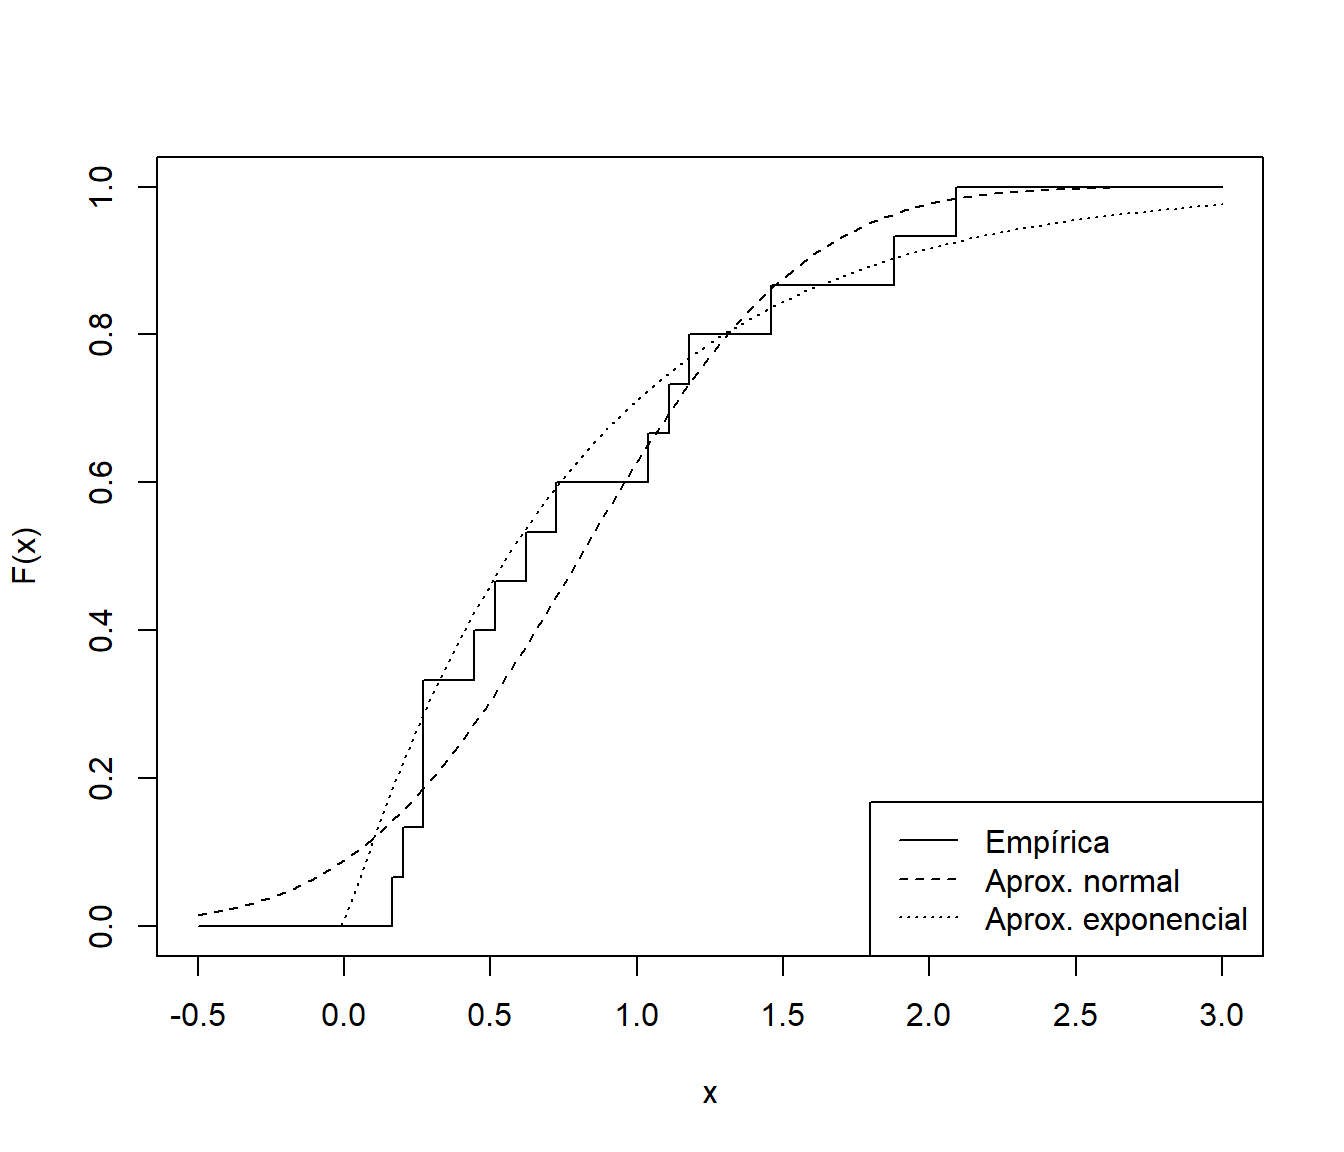
\includegraphics[width=0.7\linewidth]{04-mod_boot_unif_files/figure-latex/boot-par-aprox-1} 

}

\caption{Distribución empírica de la muestra de tiempos de vida de microorganismos y aproximaciones paramétricas.}\label{fig:boot-par-aprox}
\end{figure}

Solo tendríamos que cambiar la función que genera los datos:

\begin{Shaded}
\begin{Highlighting}[]
\NormalTok{ran.gen.exp <-}\StringTok{ }\ControlFlowTok{function}\NormalTok{(data, mle) \{}
    \CommentTok{# Función para generar muestras aleatorias exponenciales}
    \CommentTok{# mle contendrá la media de los datos originales}
\NormalTok{    out <-}\StringTok{ }\KeywordTok{rexp}\NormalTok{(}\KeywordTok{length}\NormalTok{(data), }\DecValTok{1}\OperatorTok{/}\NormalTok{mle)}
\NormalTok{    out}
\NormalTok{\}}
\end{Highlighting}
\end{Shaded}

\section{Bootstrap simetrizado}\label{bootstrap-simetrizado}

Supongamos que conocemos que la función de distribución poblacional es
simétrica entorno a cierto valor. Eso significa que existe un valor
\(c\) tal que \(F\left( c-h \right) =1-F\left( c+h \right)\) para todo
\(h>0\). Equivalentemente, una variable aleatoria es simétrica entorno a
\(c\) si su función de distribución verifica
\[F\left( x \right) = 1 - F\left( 2c - x \right)\] para todo
\(x\in \mathbb{R}\). Puede demostrarse que dicho centro de simetría,
\(c\), ha de ser la media de la distribución, \(\mu\), en caso de que
exista. Esa información (la simetría) sobre la distribución poblacional
también se debe incorporarse en el bootstrap. Así, para estimar la
función de distribución poblacional, \(F\), supuesto que es simétrica
entorno a \(\mu\), es razonable utilizar una versión simetrizada de la
distribución empírica, \(F_n^{sim}\). Ese estimador empírico simetrizado
de la función de distribución es el que otorga igual masa de
probabilidad a una muestra artificialmente construida simetrizando,
alrededor de la media muestral, la muestra original:

\[Y_i=\left\{ 
\begin{array}{ll}
X_i & \text{si } i=1,\ldots ,n \\ 
2\bar{X}-X_{i-n} &\text{si } i=n+1,\ldots ,2n
\end{array}
\right.\]

con lo cual
\[F_n^{sim}\left( x \right) =\frac{1}{2n}\sum_{i=1}^{2n}\mathbf{1}\left( Y_i\leq x \right).\]
Puede demostrarse fácilmente que
\[F_n^{sim}\left( x \right) =\frac{1}{2}\left( F_n\left( x \right)
+1-F_n\left( 2\bar{X}-x \right) \right).\]

Al diseñar el plan de remuestreo debemos utilizar \(F_n^{sim}\)
(bootstrap simetrizado), en lugar de \(F_n\) (bootstrap uniforme).

\begin{enumerate}
\def\labelenumi{\arabic{enumi}.}
\item
  Para cada \(i=1,\ldots ,n\) arrojar \(X_i^{\ast}\) a partir de
  \(F_n^{sim}\), es decir
  \(P^{\ast}\left( X_i^{\ast}=Y_j \right) =\frac{1 }{2n}\),
  \(j=1,\ldots ,2n\)
\item
  Obtener
  \(\mathbf{X}^{\ast}=\left( X_1^{\ast},\ldots ,X_n^{\ast} \right)\)
\item
  Calcular \(R^{\ast}=R\left( \mathbf{X}^{\ast},F_n^{sim} \right)\)
\end{enumerate}

Como veremos más adelante, a veces (muy poco frecuentemente) es posible
calcular exactamente la distribución bootstrap de \(R^{\ast}\). Cuando
eso no es posible, esa distribución es fácilmente aproximable por Monte
Carlo, arrojando una gran cantidad, \(B\), de réplicas de \(R^{\ast}\).
En ese caso, el algoritmo se convierte en:

\begin{enumerate}
\def\labelenumi{\arabic{enumi}.}
\item
  Para cada \(i=1,\ldots ,n\) arrojar \(X_i^{\ast}\) a partir de
  \(F_n^{sim}\)
\item
  Obtener
  \(\mathbf{X}^{\ast}=\left( X_1^{\ast},\ldots ,X_n^{\ast} \right)\)
\item
  Calcular \(R^{\ast}=R\left( \mathbf{X}^{\ast},F_n^{sim} \right)\)
\item
  Repetir \(B\) veces los pasos 1-3 para obtener las réplicas bootstrap
  \(R^{\ast (1)}\), \(\ldots\), \(R^{\ast (B)}\)
\item
  Utilizar esas réplicas bootstrap para aproximar la distribución en el
  muestreo de \(R\)
\end{enumerate}

Para llevar a cabo el paso 1 podemos proceder de dos formas
equivalentes. La primera consiste en definir explícitamente la muestra
simetrizada en torno a la media, \(\mathbf{Y}\), y luego obtener uno de
los valores de dicha muestra con equiprobabilidad. El paso 1 quedaría de
la siguiente forma:

\begin{enumerate}
\def\labelenumi{\arabic{enumi}.}
\tightlist
\item
  Para cada \(i=1,\ldots ,n\) arrojar
  \(U_i\sim \mathcal{U}\left( 0,1 \right)\) y hacer
  \(X_i^{\ast}=Y_{\left\lfloor 2nU_i\right\rfloor +1}\)
\end{enumerate}

Alternativamente podemos proceder con el paso 1 utilizando el hecho de
que la función de distribución \(F_n^{sim}\left( x \right)\) resultar
ser la distribución de una variable aleatoria obtenida en dos etapas: en
la primera etapa se genera un valor según la empírica,
\(F_n\left( x \right)\), y en la segunda se decide (con
equiprobabilidad) si el valor obtenido no se altera o bien si se refleja
alrededor de la media muestral, \(\bar{X}\). Así el paso 1 resulta:

\begin{enumerate}
\def\labelenumi{\arabic{enumi}.}
\tightlist
\item
  Para cada \(i=1,\ldots ,n\) arrojar
  \(U_i,V_i\sim \mathcal{U}\left( 0,1 \right)\). Si
  \(V_i\leq \frac{1}{2}\) entonces hacer
  \(X_i^{\ast}=X_{\left\lfloor nU_i\right\rfloor +1}\) y en caso
  contrario hacer
  \(X_i^{\ast}=2\overline{X }-X_{\left\lfloor nU_i\right\rfloor +1}\)
\end{enumerate}

La utilización de \(F_n^{sim}\left( x \right)\) en lugar de
\(F_n\left( x \right)\) altera las propiedades conocidas de la
distribución (empírica) de la que se remuestrea en el bootstrap
uniforme. Así, en primer lugar, \(F_n^{sim}\left( x \right)\) es
simétrica (como se desea) con lo cual todos los momentos impares de esta
distribución con respecto a \(\bar{X}\) son cero. En particular la media
de \(F_n^{sim}\left(x \right)\) es \[\begin{aligned}
\int x~dF_n^{sim}\left( x \right) &= \frac{1}{2n}\sum_{i=1}^{2n}Y_i=\frac{
1}{2n}\left[ \sum_{i=1}^{n}X_i+\sum_{i=1}^{n}\left( 2\bar{X}
-X_i \right) \right] \\
&= \frac{1}{2n}\left( n\bar{X}+2n\bar{X}-n\bar{X} \right) =
\bar{X}.\end{aligned}\] También se conservan los momentos centrales de
orden par:

\[\begin{aligned}
\int \left( x-\bar{X} \right)^{2k}~dF_n^{sim}\left( x \right) &= \frac{
1}{2n}\sum_{i=1}^{2n}\left( Y_i-\bar{X} \right)^{2k} \\
&= \frac{1}{2n}\left[ \sum_{i=1}^{n}\left( X_i-\bar{X} \right)
^{2k}+\sum_{i=1}^{n}\left[ \left( 2\bar{X}-X_i \right) -\bar{X}
\right]^{2k}\right] \\
&= \frac{1}{2n}\left[ \sum_{i=1}^{n}\left( X_i-\bar{X} \right)
^{2k}+\sum_{i=1}^{n}\left( \bar{X}-X_i \right)^{2k}\right] \\
&= \frac{1}{n}\sum_{i=1}^{n}\left( X_i-\bar{X} \right)^{2k}.
\end{aligned}\]

En particular, la varianza de \(F_n^{sim}\left( x \right)\) coincide con
la de \(F_n\left( x \right)\), que es \(S_n^2\).

En general, cuando la distribución de partida es simétrica, es más
adecuado utilizar el bootstrap simetrizado que el bootstrap uniforme.
Aún así, cuando se realiza inferencia sobre algún estadístico (como
\(\sqrt{n}(\bar{X}-\mu)/\sigma\)) cuya distribución asintótica ya es
simétrica (como la normal), la aproximación bootstrap uniforme para
distribuciones de partida simétricas, ya es especialmente buena y, por
tanto, la ganancia del bootstrap simétrizado aporta una mejora difícil
de detectar en la práctica. Ese no es el caso de otros estadísticos
(como los asociados a inferencia sobre la varianza) con distribución más
alejada de la simetría.

\BeginKnitrBlock{exercise}[Inferencia sobre la media con varianza conocida empleando bootstrap simetrizado]
\protect\hypertarget{exr:media-dt-conocida-sim}{}{\label{exr:media-dt-conocida-sim}
\iffalse (Inferencia sobre la media con varianza conocida empleando
bootstrap simetrizado) \fi{} } Modificar adecuadamente el código del
Ejemplo \ref{exm:media-dt-conocida}, para implementar un método
bootstrap simetrizado, con el objeto de calcular un intervalo de
confianza para la media con desviación típica conocida. Qué diferencias
se observan entre los intervalos obtenidos por el bootstrap uniforme y
por el simetrizado?
\EndKnitrBlock{exercise}

\section{Bootstrap suavizado}\label{cap4-boot-suav}

Cuando la distribución poblacional, \(F\), es continua es lógico
incorporar dicha información al bootstrap. Eso significa que la función
de distribución tiene una función de densidad asociada, relacionadas
mediante la expresión:
\(f\left( x \right) =F^{\prime}\left( x \right)\). Para ello, debemos
utilizar un método bootstrap que remuestree de un universo bootstrap
continuo. En otras palabras debemos utilizar un estimador de la función
de densidad y remuestrear de él.

Pasamos a considerar brevemente el problema de estimar, no
paramétricamente, la función de densidad, \(f\), de una población, a
partir de una muestra, \(\left( X_1,X_2,\ldots ,X_n \right)\),
procedente de la misma. En ese contexto es bien conocido el método
histograma (basado en el cual sería posible idear un método bootstrap)
aunque es más recomendable utilizar el estimador tipo núcleo propuesto
por Parzen (1962) y Rosenblatt (1956), que viene dado por

\[\hat{f}_{h}\left( x \right) =\frac{1}{nh}\sum_{i=1}^{n}K\left( \frac{x-X_i}{
h} \right) =\frac{1}{n}\sum_{i=1}^{n}K_{h}\left( x-X_i \right),\]

donde \[K_{h}\left( u \right) =\frac{1}{h}K\left( \frac{u}{h} \right),\]
\(K\) es una función núcleo (normalmente una densidad simétrica en torno
al cero) y \(h>0\) es una parámetro de suavizado, llamado ventana, que
regula el tamaño del entorno que se usa para llevar a cabo la
estimación. Este estimador generaliza el bien conocido histograma y, más
concretamente, su versión histograma móvil. Así, eligiendo como función
\(K\) la densidad de una \(\mathcal{U}\left( -1,1 \right)\), el
estimador de Parzen-Rosenblatt resulta: \[\begin{aligned}
\frac{1}{nh}\sum_{i=1}^{n}\frac{1}{2}\mathbf{1}\left\{ \frac{x-X_i}{h}\in
\left( -1,1 \right) \right\} &= \frac{1}{2nh}\sum_{i=1}^{n}\mathbf{1}\left\{
X_i\in \left( x-h,x+h \right) \right\} \\
&= \frac{\#\left\{ X_i\in \left( x-h,x+h \right) \right\} }{2nh},
\end{aligned}\] que no es más que la frecuencia relativa de datos
\(X_i\) en el intervalo \(\left( x-h,x+h \right)\) dividida entre la
longitud del intervalo en cuestión (\(2h\)).

Es habitual exigir que la función núcleo \(K\) sea no negativa y su
integral sea uno:
\[K\left( u \right) \geq 0,~\forall u,~\int_{-\infty }^{\infty }K\left(u \right) du=1.\]
Además también es frecuente exigir que \(K\) sea una función simétrica
(\(K\left( -u \right) =K\left( u \right)\)).

Aunque la elección de la función \(K\) no tiene gran impacto en las
propiedades del estimador (salvo sus condiciones de regularidad:
continuidad, diferenciabilidad, etc.) la elección del parámetro de
suavizado sí es muy importante para una correcta estimación. En otras
palabras, el tamaño del entorno usado para la estimación no paramétrica
debe ser adecuado (ni demasiado grande ni demasiado pequeño).

En \texttt{R} podemos emplear la función \texttt{density()} del paquete
base para obtener una estimación tipo núcleo de la densidad (con la
ventana determinada por el parámetro \texttt{bw}), aunque podríamos
emplear implementaciones de otros paquetes (como el paquete \texttt{ks},
que admite estimación multidimensional). Por ejemplo, considerando el
conjunto de datos \texttt{precip} (que contiene el promedio de
precipitación, en pulgadas de lluvia, de 70 ciudades de Estados Unidos),
podríamos utilizar el siguiente código {[}Figura \ref{fig:density}{]}:

\begin{Shaded}
\begin{Highlighting}[]
\NormalTok{x <-}\StringTok{ }\NormalTok{precip}
\NormalTok{npden <-}\StringTok{ }\KeywordTok{density}\NormalTok{(x)}
\CommentTok{# npden <- density(x, bw = "SJ")}

\CommentTok{# plot(npden)}
\NormalTok{bandwidth <-}\StringTok{ }\NormalTok{npden}\OperatorTok{$}\NormalTok{bw}
\KeywordTok{hist}\NormalTok{(x, }\DataTypeTok{freq =} \OtherTok{FALSE}\NormalTok{, }\DataTypeTok{main =} \StringTok{"Kernel density estimation"}\NormalTok{, }
     \DataTypeTok{xlab =} \KeywordTok{paste}\NormalTok{(}\StringTok{"Bandwidth ="}\NormalTok{, }\KeywordTok{formatC}\NormalTok{(bandwidth)), }\DataTypeTok{lty =} \DecValTok{2}\NormalTok{, }
     \DataTypeTok{border =} \StringTok{"darkgray"}\NormalTok{, }\DataTypeTok{xlim =} \KeywordTok{c}\NormalTok{(}\DecValTok{0}\NormalTok{, }\DecValTok{80}\NormalTok{), }\DataTypeTok{ylim =} \KeywordTok{c}\NormalTok{(}\DecValTok{0}\NormalTok{, }\FloatTok{0.08}\NormalTok{))}
\KeywordTok{lines}\NormalTok{(npden, }\DataTypeTok{lwd =} \DecValTok{2}\NormalTok{)}
\KeywordTok{rug}\NormalTok{(x, }\DataTypeTok{col =} \StringTok{"darkgray"}\NormalTok{)}
\end{Highlighting}
\end{Shaded}

\begin{figure}[!htb]

{\centering 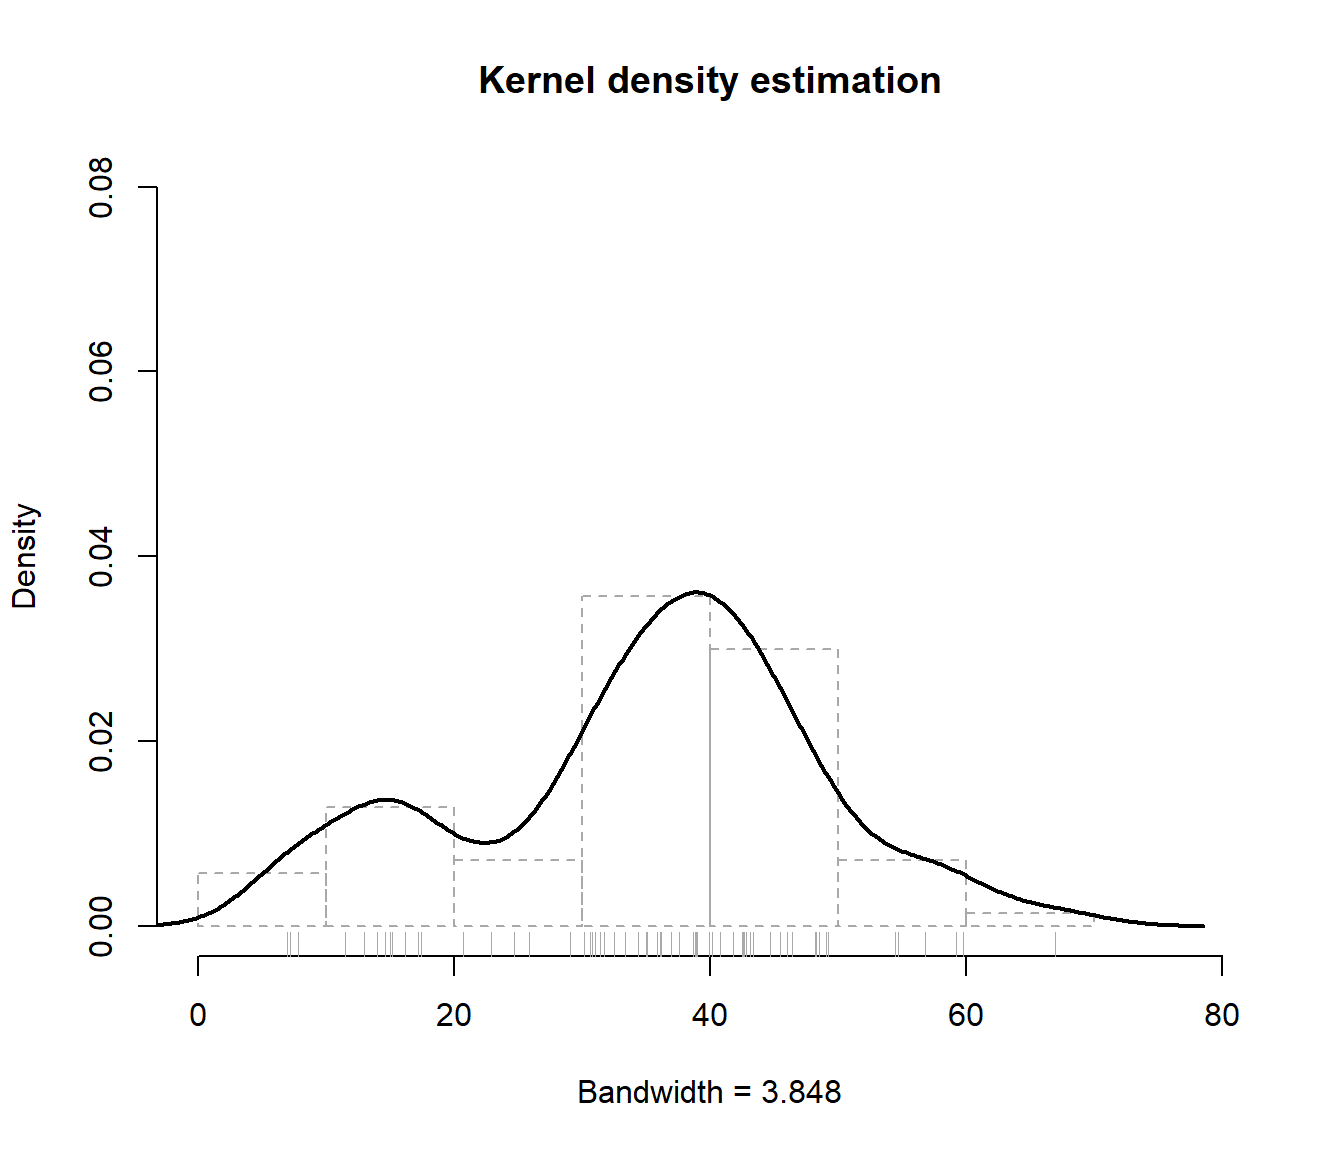
\includegraphics[width=0.7\linewidth]{04-mod_boot_unif_files/figure-latex/density-1} 

}

\caption{Estimación tipo núcleo de la densidad de `precip`. }\label{fig:density}
\end{figure}

La sensibilidad del estimador tipo núcleo al parámetro de suavizado
puede observarse ejecutando el siguiente código (ver Figura
\ref{fig:bandwidth-movie},
\href{./bandwidth-movie.gif}{bandwidth-movie.gif}):

\begin{Shaded}
\begin{Highlighting}[]
\NormalTok{bws <-}\StringTok{ }\DecValTok{2}\OperatorTok{^}\KeywordTok{seq}\NormalTok{(}\KeywordTok{log2}\NormalTok{(bandwidth }\OperatorTok{*}\StringTok{ }\FloatTok{0.01}\NormalTok{), }\KeywordTok{log2}\NormalTok{(bandwidth }\OperatorTok{*}\StringTok{ }\DecValTok{20}\NormalTok{), }\DataTypeTok{len =} \DecValTok{50}\NormalTok{)}
\NormalTok{bws <-}\StringTok{ }\KeywordTok{c}\NormalTok{(bws, }\KeywordTok{rev}\NormalTok{(bws))}
\ControlFlowTok{for}\NormalTok{ (bw }\ControlFlowTok{in}\NormalTok{ bws)}
  \KeywordTok{plot}\NormalTok{(}\KeywordTok{density}\NormalTok{(x, }\DataTypeTok{bw =}\NormalTok{ bw) , }\DataTypeTok{main =} \StringTok{"Kernel density estimation"}\NormalTok{, }
         \DataTypeTok{xlab =} \KeywordTok{paste}\NormalTok{(}\StringTok{"Bandwidth ="}\NormalTok{, }\KeywordTok{formatC}\NormalTok{(bw)), }
         \DataTypeTok{xlim =} \KeywordTok{c}\NormalTok{(}\DecValTok{0}\NormalTok{, }\DecValTok{80}\NormalTok{), }\DataTypeTok{ylim =} \KeywordTok{c}\NormalTok{(}\DecValTok{0}\NormalTok{, }\FloatTok{0.08}\NormalTok{))}
\end{Highlighting}
\end{Shaded}

\begin{figure}[!htb]

{\centering \includegraphics[width=0.7\linewidth]{04-mod_boot_unif_files/figure-latex/bandwidth-movie-1} 

}

\caption{Efecto de cambio en la ventana en la estimación tipo núcleo de la densidad.}\label{fig:bandwidth-movie}
\end{figure}

La función de distribución asociada al estimador tipo núcleo de la
función de densidad viene dada por \[\begin{aligned}
\hat{F}_{h}\left( x \right) &= \int_{-\infty }^{x}\hat{f}_{h}\left( y \right) dy
=\int_{-\infty }^{x}\frac{1}{n}\sum_{i=1}^{n}\frac{1}{h}
K\left( \frac{y-X_i}{h} \right) dy \\
&= \frac{1}{nh}\sum_{i=1}^{n}\int_{-\infty }^{x}
K\left( \frac{y-X_i}{h} \right) dy \\
&= \frac{1}{n}\sum_{i=1}^{n}\int_{-\infty }^{\frac{x-X_i}{h}}K\left( u \right) du
=\frac{1}{n}\sum_{i=1}^{n}\mathbb{K}\left( \frac{x-X_i}{h} \right)
\end{aligned}\] donde \(\mathbb{K}\) es la función de distribución
asociada al núcleo \(K\), es decir
\[\mathbb{K}\left( t \right) =\int_{-\infty }^{t}K\left(
u \right) du.\]

El método bootstrap suavizado procede de la siguiente forma:

\begin{enumerate}
\def\labelenumi{\arabic{enumi}.}
\item
  A partir de la muestra \(\left( X_1,X_2,\ldots ,X_n \right)\) y
  utilizando un valor \(h>0\) como parámetro de suavizado, se calcula el
  estimador de Parzen-Rosenblatt \(\hat{f}_{h}\)
\item
  Se arrojan remuestras bootstrap
  \(\mathbf{X}^{\ast}=\left( X_1^{\ast},X_2^{\ast},\ldots ,X_n^{\ast} \right)\)
  a partir de la densidad \(\hat{f}_{h}\)
\item
  Calcular \(R^{\ast}=R\left( \mathbf{X}^{\ast},\hat{F}_{h} \right)\)
\item
  Repetir \(B\) veces los pasos 2-3 para obtener las réplicas bootstrap
  \(R^{\ast (1)}\), \(\ldots\), \(R^{\ast (B)}\)
\end{enumerate}

Para llevar a cabo un bootstrap que remuestree a partir del estimador
\(\hat{f}_{h}\left( x \right)\) es útil pensar en dicho estimador como
una combinación lineal convexa de funciones de densidad,
\(K_{h}\left( x-X_i \right)\), cada una con coeficiente \(\frac{1}{n}\)
en dicha combinación lineal. Gracias a esa representación podemos
simular valores, \(X^{\ast}\), procedentes de
\(\hat{f}_{h}\left( x \right)\) en dos pasos.

En un primer paso elegiremos (aleatoriamente y con equiprobabilidad)
cuál de los índices \(i\in \left\{ 1,\ldots ,n\right\}\) vamos a
considerar y en un segundo paso simularemos \(X^{\ast}\) a partir de la
densidad \(K_{h}\left( \cdot -X_i \right)\). Esta última fase puede
relacionarse fácilmente con la simulación de un valor, \(V\), con
densidad \(K\), sin más que hacer \(X_i+hV\). Así, el paso 2 del
algoritmo previo puede llevarse a cabo mediante el siguiente
procedimiento:

\begin{enumerate}
\def\labelenumi{\arabic{enumi}.}
\setcounter{enumi}{1}
\tightlist
\item
  Para cada \(i=1,\ldots ,n\) arrojar
  \(U_i\sim \mathcal{U}\left( 0,1 \right)\) y \(V_i\) con densidad \(K\)
  y hacer \(X_i^{\ast}=X_{\left\lfloor nU_i\right\rfloor +1}+hV_i\)
\end{enumerate}

La equivalencia de ambas presentaciones del paso 2 viene dada por el
siguiente razonamiento. Denotando
\(U\sim \mathcal{U}\left( 0,1 \right)\),
\(I=\left\lfloor nU\right\rfloor +1\) y \(V\sim K\), independiente de
\(U\), se tiene:

\[\begin{aligned}
P^{\ast}\left( X^{\ast}\leq x \right) &= \sum_{i=1}^{n}P^{\ast}\left(
\left. X^{\ast}\leq x\right\vert _{I=i} \right) P^{\ast}\left( I=i \right) \\
&= \sum_{i=1}^{n}P^{\ast}\left( \left. X_i+hV\leq x\right\vert
_{I=i} \right) P^{\ast}\left( I=i \right) \\
&= \sum_{i=1}^{n}P^{\ast}\left( \left. V\leq \frac{x-X_i}{h}
\right\vert _{X_i} \right) \frac{1}{n}=\frac{1}{n}\sum_{i=1}^{n}\mathbb{K}
\left( \frac{x-X_i}{h} \right),
\end{aligned}\]

cuya función de densidad es, como ya sabemos,
\(\hat{f}_{h}\left( x \right)\). Esto justifica la presentación
alternativa del paso 2, de forma que el bootstrap suavizado puede
pensarse, a partir del bootstrap uniforme
(\(X_i^{\ast}=X_{\left\lfloor nU_i\right\rfloor +1}\)) añadiendo al
mismo una perturbación (\(hV_i\)) cuya magnitud viene dada por el
parámetro de suavizado (\(h\)) y cuya forma imita a la de una variable
aleatoria (\(V_i\)) con densidad \(K\).

Por ejemplo, la función \texttt{density()} emplea por defecto un núcleo
gaussiano, y como se muestra en la ayuda de esta función, podemos
emplear un código como el siguiente para obtener \texttt{nsim}
simulaciones (ver Figura \ref{fig:density-sim}):

\begin{Shaded}
\begin{Highlighting}[]
\NormalTok{## simulation from a density() fit:}
\CommentTok{# a kernel density fit is an equally-weighted mixture.}
\NormalTok{nsim <-}\StringTok{ }\FloatTok{1e6}
\KeywordTok{set.seed}\NormalTok{(}\DecValTok{1}\NormalTok{)}
\CommentTok{# x_boot <- sample(x, nsim, replace = TRUE)}
\CommentTok{# x_boot <- x_boot + bandwidth * rnorm(nsim)}
\NormalTok{x_boot <-}\StringTok{ }\KeywordTok{rnorm}\NormalTok{(nsim, }\KeywordTok{sample}\NormalTok{(x, nsim, }\DataTypeTok{replace =} \OtherTok{TRUE}\NormalTok{), bandwidth)}

\KeywordTok{plot}\NormalTok{(npden)}
\KeywordTok{lines}\NormalTok{(}\KeywordTok{density}\NormalTok{(x_boot), }\DataTypeTok{col =} \StringTok{"blue"}\NormalTok{, }\DataTypeTok{lwd =} \DecValTok{2}\NormalTok{, }\DataTypeTok{lty =} \DecValTok{2}\NormalTok{)}
\end{Highlighting}
\end{Shaded}

\begin{figure}[!htb]

{\centering 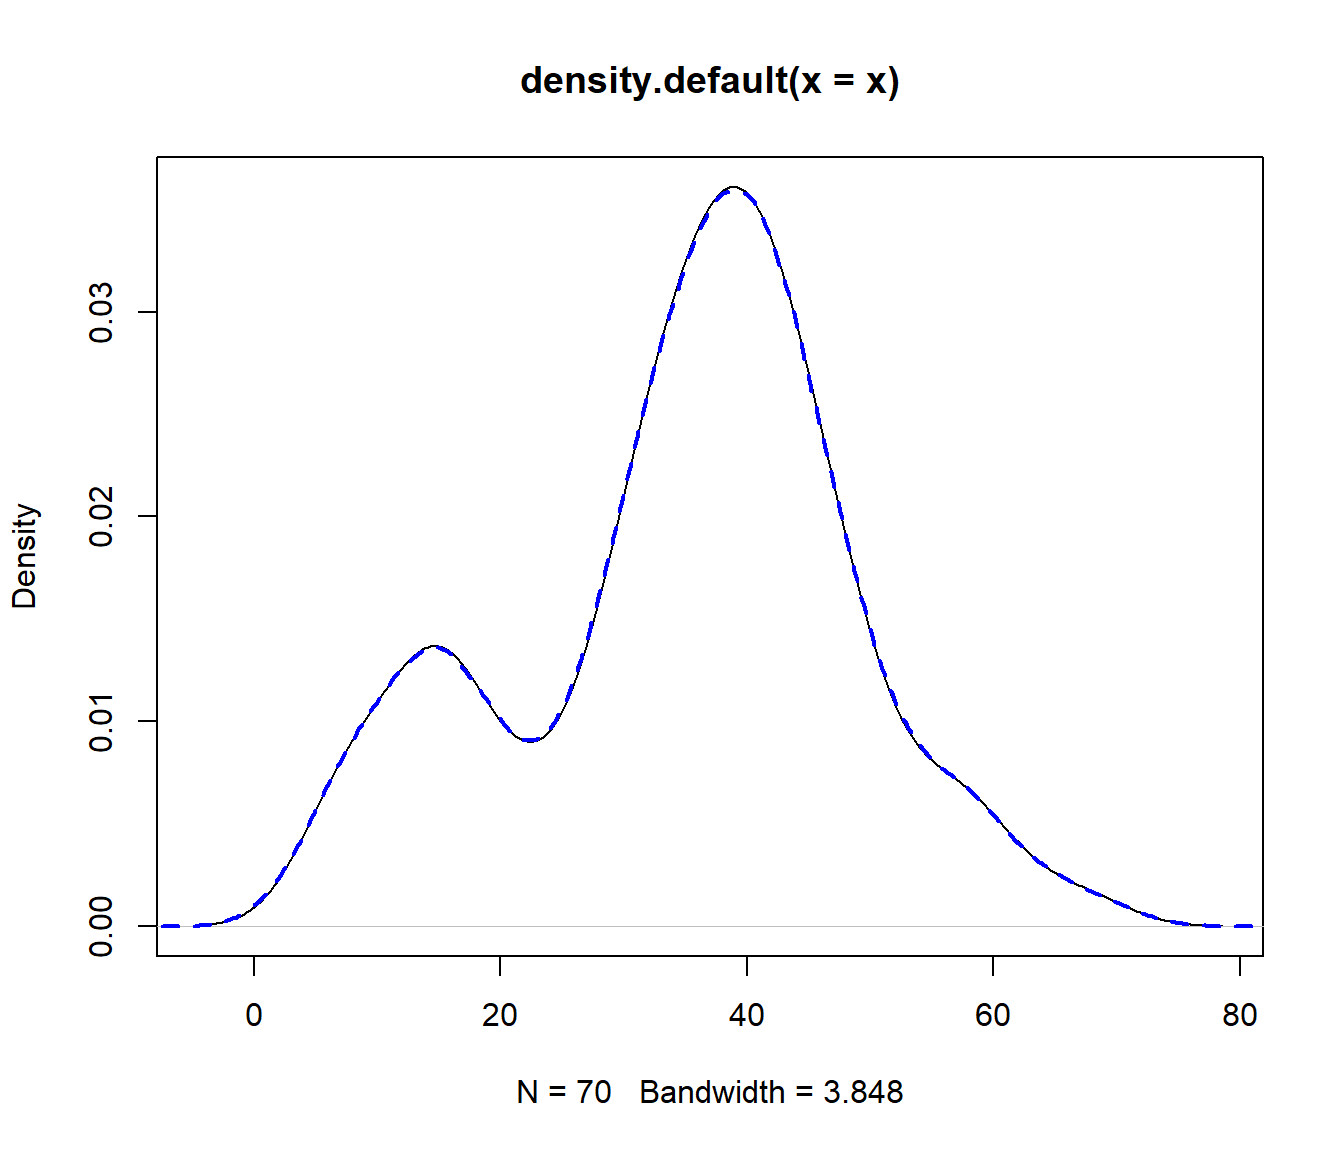
\includegraphics[width=0.7\linewidth]{04-mod_boot_unif_files/figure-latex/density-sim-1} 

}

\caption{Estimaciónes tipo núcleo de las densidades de `precip` y de una simulación.}\label{fig:density-sim}
\end{figure}

Es fácil percatarse de que los posibles valores que puede tomar una
observación \(X_i^{\ast}\) de cada remuestra bootstrap son infinitos,
pues la variable \(V\) puede tomar infinitos posibles valores, según la
densidad de probabilidad \(K\). Esto significa que la distribución en el
remuestreo de la remuestra bootstrap, \(\mathbf{X}^{\ast}\), es mucho
más complicada que para el bootstrap uniforme. En particular no es
discreta y por tanto no puede caracterizarse a partir de vectores de
remuestreo sobre la muestra original. Un problema importante es la
elección del parámetro de suavizado, \(h\), en este procedimiento de
remuestreo. En la práctica es razonable elegir \(h\) como un valor
bastante pequeño, en relación con la desviación típica de la muestra. Es
fácil observar que en el caso extremo \(h=0\) este método de remuestreo
se reduce al bootstrap uniforme.

\BeginKnitrBlock{example}[Inferencia sobre la media con varianza conocida, continuación]
\protect\hypertarget{exm:media-dt-conocida-suav}{}{\label{exm:media-dt-conocida-suav}
\iffalse (Inferencia sobre la media con varianza conocida, continuación)
\fi{} } Continuando con el ejemplo de tiempo de vida de microorganismos,
podemos modificar fácilmente el código mostrado en el Ejemplo
\ref{exm:media-dt-conocida}, para implementar bootstrap suavizado con
función núcleo gaussiana, para calcular un intervalo de confianza para
la media poblacional con desviación típica conocida:
\EndKnitrBlock{example}

\begin{Shaded}
\begin{Highlighting}[]
\NormalTok{muestra <-}\StringTok{ }\KeywordTok{c}\NormalTok{(}\FloatTok{0.143}\NormalTok{, }\FloatTok{0.182}\NormalTok{, }\FloatTok{0.256}\NormalTok{, }\FloatTok{0.26}\NormalTok{, }\FloatTok{0.27}\NormalTok{, }\FloatTok{0.437}\NormalTok{, }\FloatTok{0.509}\NormalTok{, }
             \FloatTok{0.611}\NormalTok{, }\FloatTok{0.712}\NormalTok{, }\FloatTok{1.04}\NormalTok{, }\FloatTok{1.09}\NormalTok{, }\FloatTok{1.15}\NormalTok{, }\FloatTok{1.46}\NormalTok{, }\FloatTok{1.88}\NormalTok{, }\FloatTok{2.08}\NormalTok{)}
\NormalTok{n <-}\StringTok{ }\KeywordTok{length}\NormalTok{(muestra)}
\NormalTok{sigma <-}\StringTok{ }\FloatTok{0.6}

\NormalTok{alfa <-}\StringTok{ }\FloatTok{0.05}
\NormalTok{x_barra <-}\StringTok{ }\KeywordTok{mean}\NormalTok{(muestra)}

\CommentTok{# Remuestreo}
\KeywordTok{set.seed}\NormalTok{(}\DecValTok{1}\NormalTok{)}
\NormalTok{B <-}\StringTok{ }\DecValTok{1000}
\CommentTok{# h <- 1e-08}
\NormalTok{h <-}\StringTok{ }\KeywordTok{bw.SJ}\NormalTok{(muestra)}\OperatorTok{/}\DecValTok{2}
\NormalTok{estadistico_boot <-}\StringTok{ }\KeywordTok{numeric}\NormalTok{(B)}
\ControlFlowTok{for}\NormalTok{ (k }\ControlFlowTok{in} \DecValTok{1}\OperatorTok{:}\NormalTok{B) \{}
    \CommentTok{# remuestra <- sample(muestra, n, replace = TRUE)}
    \CommentTok{# remuestrasu <- remuestra + h * rnorm(n, 0, 1)}
\NormalTok{    remuestrasu <-}\StringTok{ }\KeywordTok{rnorm}\NormalTok{(n, }\KeywordTok{sample}\NormalTok{(muestra, n, }\DataTypeTok{replace =} \OtherTok{TRUE}\NormalTok{), h)}
\NormalTok{    x_barra_boot <-}\StringTok{ }\KeywordTok{mean}\NormalTok{(remuestrasu)}
\NormalTok{    estadistico_boot[k] <-}\StringTok{ }\KeywordTok{sqrt}\NormalTok{(n) }\OperatorTok{*}\StringTok{ }\NormalTok{(x_barra_boot }\OperatorTok{-}\StringTok{ }\NormalTok{x_barra)}\OperatorTok{/}\NormalTok{sigma}
\NormalTok{\}}

\CommentTok{# Aproximación bootstrap de los ptos críticos}
\NormalTok{pto_crit <-}\StringTok{ }\KeywordTok{quantile}\NormalTok{(estadistico_boot, }\KeywordTok{c}\NormalTok{(alfa}\OperatorTok{/}\DecValTok{2}\NormalTok{, }\DecValTok{1} \OperatorTok{-}\StringTok{ }\NormalTok{alfa}\OperatorTok{/}\DecValTok{2}\NormalTok{))}

\CommentTok{# Construcción del IC}
\NormalTok{ic_inf_boot <-}\StringTok{ }\NormalTok{x_barra }\OperatorTok{-}\StringTok{ }\NormalTok{pto_crit[}\DecValTok{2}\NormalTok{] }\OperatorTok{*}\StringTok{ }\NormalTok{sigma}\OperatorTok{/}\KeywordTok{sqrt}\NormalTok{(n)}
\NormalTok{ic_sup_boot <-}\StringTok{ }\NormalTok{x_barra }\OperatorTok{-}\StringTok{ }\NormalTok{pto_crit[}\DecValTok{1}\NormalTok{] }\OperatorTok{*}\StringTok{ }\NormalTok{sigma}\OperatorTok{/}\KeywordTok{sqrt}\NormalTok{(n)}
\NormalTok{IC_boot <-}\StringTok{ }\KeywordTok{c}\NormalTok{(ic_inf_boot, ic_sup_boot)}
\KeywordTok{names}\NormalTok{(IC_boot) <-}\StringTok{ }\KeywordTok{paste0}\NormalTok{(}\DecValTok{100}\OperatorTok{*}\KeywordTok{c}\NormalTok{(alfa}\OperatorTok{/}\DecValTok{2}\NormalTok{, }\DecValTok{1}\OperatorTok{-}\NormalTok{alfa}\OperatorTok{/}\DecValTok{2}\NormalTok{), }\StringTok{"%"}\NormalTok{)}
\NormalTok{IC_boot}
\end{Highlighting}
\end{Shaded}

\begin{verbatim}
##      2.5%     97.5% 
## 0.4592311 1.1103890
\end{verbatim}

Con el paquete \texttt{boot}, la recomendación es implementarlo como un
bootstrap paramétrico:

\begin{Shaded}
\begin{Highlighting}[]
\KeywordTok{library}\NormalTok{(boot)}
\NormalTok{ran.gen.smooth <-}\StringTok{ }\ControlFlowTok{function}\NormalTok{(data, mle) \{}
    \CommentTok{# Función para generar muestras aleatorias mediante }
    \CommentTok{# bootstrap suavizado con función núcleo gaussiana,}
    \CommentTok{# mle contendrá la ventana.}
\NormalTok{    n <-}\StringTok{ }\KeywordTok{length}\NormalTok{(data)}
\NormalTok{    h <-}\StringTok{ }\NormalTok{mle}
\NormalTok{    out <-}\StringTok{ }\KeywordTok{rnorm}\NormalTok{(n, }\KeywordTok{sample}\NormalTok{(data, n, }\DataTypeTok{replace =} \OtherTok{TRUE}\NormalTok{), h)}
\NormalTok{    out}
\NormalTok{\}}

\NormalTok{statistic <-}\StringTok{ }\ControlFlowTok{function}\NormalTok{(data)\{}
    \KeywordTok{c}\NormalTok{(}\KeywordTok{mean}\NormalTok{(data), sigma}\OperatorTok{^}\DecValTok{2}\OperatorTok{/}\KeywordTok{length}\NormalTok{(data))}
\NormalTok{\}}

\KeywordTok{set.seed}\NormalTok{(}\DecValTok{1}\NormalTok{)}
\NormalTok{res.boot <-}\StringTok{ }\KeywordTok{boot}\NormalTok{(muestra, statistic, }\DataTypeTok{R =}\NormalTok{ B, }\DataTypeTok{sim =} \StringTok{"parametric"}\NormalTok{,}
                 \DataTypeTok{ran.gen =}\NormalTok{ ran.gen.smooth, }\DataTypeTok{mle =}\NormalTok{ h)}

\KeywordTok{boot.ci}\NormalTok{(res.boot, }\DataTypeTok{type =} \StringTok{"stud"}\NormalTok{)}
\end{Highlighting}
\end{Shaded}

\begin{verbatim}
## BOOTSTRAP CONFIDENCE INTERVAL CALCULATIONS
## Based on 1000 bootstrap replicates
## 
## CALL : 
## boot.ci(boot.out = res.boot, type = "stud")
## 
## Intervals : 
## Level    Studentized     
## 95%   ( 0.4580,  1.1132 )  
## Calculations and Intervals on Original Scale
\end{verbatim}

\section{Bootstrap ponderado y bootstrap
sesgado}\label{bootstrap-ponderado-y-bootstrap-sesgado}

Mediante el nombre bootstrap ponderado se incluyen todos aquellos
métodos de remuestreo bootstrap en los que la distribución de la que se
remuestrea es discreta y asigna probabilidades sólo a los datos de la
muestra:
\[\hat{F}\left( X_i \right) -\hat{F}\left( X_i^{-} \right) = p_i
\text{, para }i=1,\ldots, n\] siendo \(p_i\geq 0\) y
\(\sum_{i=1}^{n}p_i=1\). En el caso particular \(p_i= \frac{1}{n}\) para
todo \(i=1,\ldots ,n\), se tiene el bootstrap uniforme. Veremos más
adelante casos particulares de métodos bootstrap ponderados en el
contexto de datos censurados y también para datos dependientes.

El bootstrap ponderado da lugar al bootstrap sesgado cuando los pesos,
\(p_i\), se eligen de forma que el vector \(\mathbf{p}\) minimice la
distancia al vector de pesos del bootstrap uniforme
\(\left( \frac{1}{n},\ldots ,\frac{1}{n} \right)\), sujeto a una serie
de restricciones inherentes al problema en estudio. Este método fue
propuesto por Hall (1998).

\section{Deficiencias del bootstrap
uniforme}\label{deficiencias-del-bootstrap-uniforme}

Supongamos un contexto paramétrico en el que la distribución
poblacional, \(F\), es la \(\mathcal{U}\left( 0,\theta \right)\).
Nuestro interés será hacer inferencia acerca del parámetro \(\theta\),
para lo cual, dada una muestra observada,
\(\mathbf{X}=\left( X_1,X_2,\ldots ,X_n \right)\), consideraremos el
estimador máximo verosímil en este contexto: \(\hat{\theta}=X_{(n)}\).
Para realizar dicha inferencia estaremos interesados en aproximar la
distribución de \(R\left( \mathbf{X},F \right) =\hat{\theta}-\theta\)

La función de distribución en el muestreo, \(G\left( x \right)\), de
\(\hat{\theta}\) puede calcularse de forma sencilla:\[\begin{aligned}
G\left( x \right) &= P\left( \hat{\theta}\leq x \right) =P\left( X_{\left(
n \right)}\leq x \right) =P\left( X_i\leq x\,,\forall i\in \left\{ 1,\ldots
n\right\} \right) \\
&= \prod_{i=1}^{n}P\left( X_i\leq x \right) =F\left( x \right)^{n}=\left( 
\frac{x}{\theta } \right)^{n},\text{ si }x\in \left[ 0,\theta \right]\end{aligned}\]

con lo cual su función de densidad viene dada por
\[g\left( x \right) =\frac{n}{\theta }\left( \frac{x}{\theta } \right)^{n-1},
\text{ si }x\in \left[ 0,\theta \right] .\] Tomando, por ejemplo,
\(\theta =1\) y \(n=50\), esta función de densidad resulta {[}Figura
\ref{fig:den-max}{]}:

\begin{Shaded}
\begin{Highlighting}[]
\NormalTok{theta <-}\StringTok{ }\DecValTok{1}
\NormalTok{n <-}\StringTok{ }\DecValTok{50}
\KeywordTok{curve}\NormalTok{(n}\OperatorTok{/}\NormalTok{theta }\OperatorTok{*}\StringTok{ }\NormalTok{(x}\OperatorTok{/}\NormalTok{theta)}\OperatorTok{^}\NormalTok{(n }\OperatorTok{-}\StringTok{ }\DecValTok{1}\NormalTok{), }\DecValTok{0}\NormalTok{, theta, }\DataTypeTok{ylab =} \StringTok{"Density"}\NormalTok{)}
\end{Highlighting}
\end{Shaded}

\begin{figure}[!htb]

{\centering 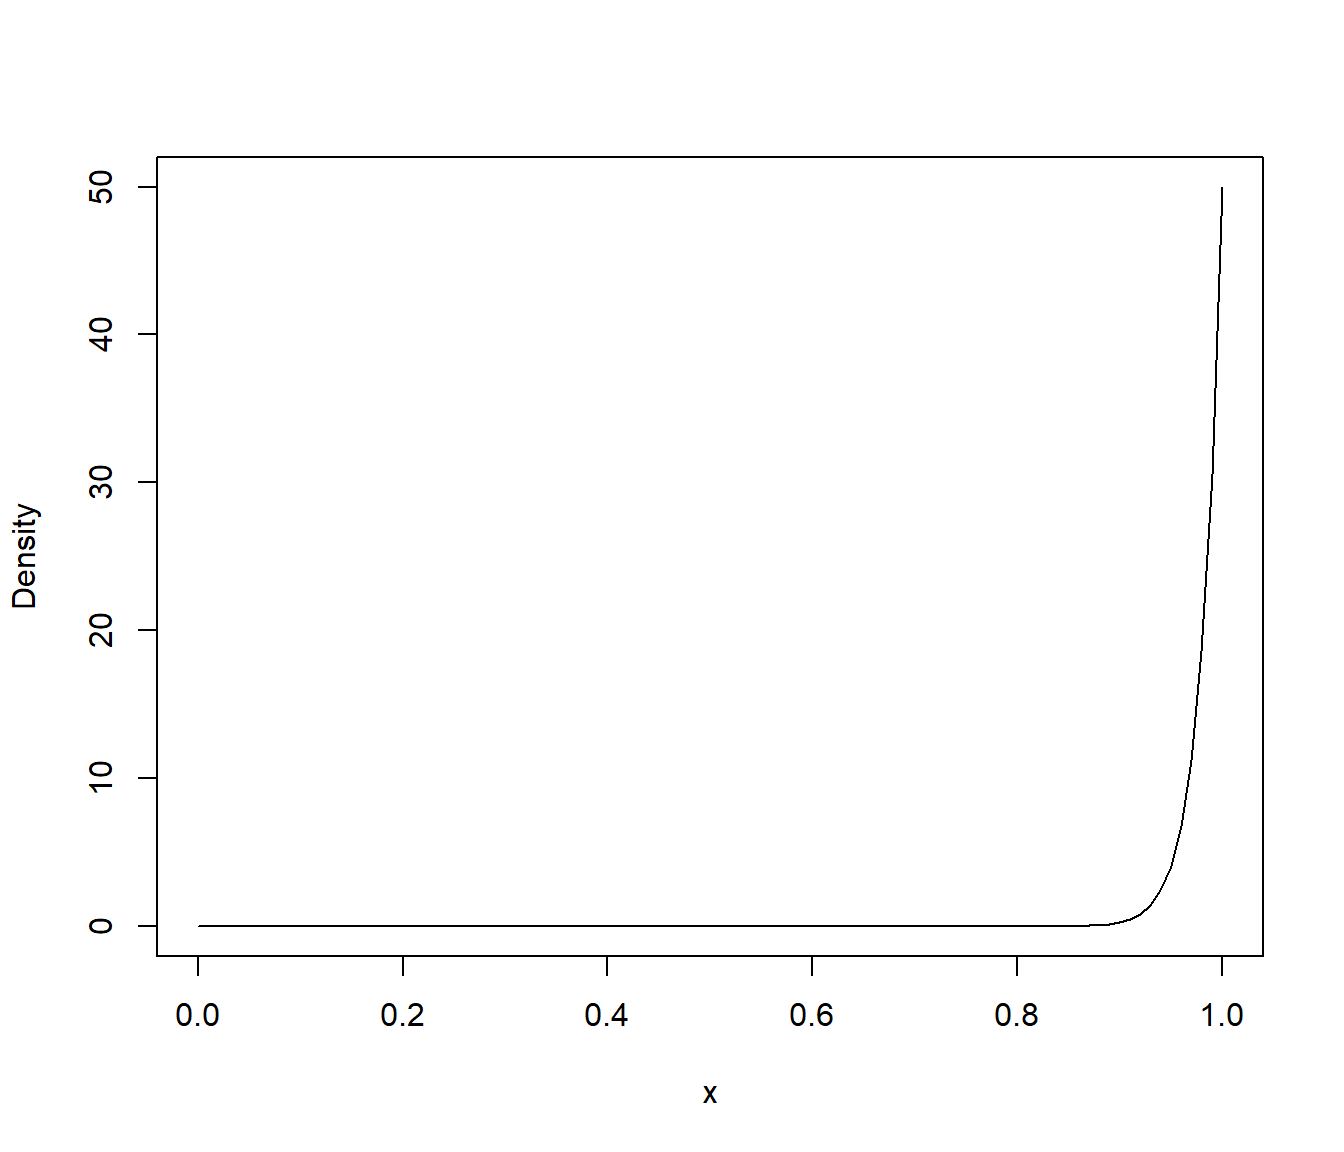
\includegraphics[width=0.7\linewidth]{04-mod_boot_unif_files/figure-latex/den-max-1} 

}

\caption{Función de densidad del máximo de una muestra procedente de una uniforme.}\label{fig:den-max}
\end{figure}

Como consecuencia podemos hallar fácilmente el sesgo del estimador
\(\hat{\theta}\), ya que
\[E\left( \hat{\theta} \right) =\int_{0}^{\theta }x\frac{n}{\theta }\left( 
\frac{x}{\theta } \right)^{n-1}dx=\left[ \frac{n}{n+1}\frac{x^{n+1}}{\theta
^{n}}\right] _{x=0}^{x=\theta }=\frac{n}{n+1}\theta ,\] con lo cual
\[Sesgo\left( \hat{\theta} \right) =E\left( \hat{\theta} \right)
-\theta = -\frac{\theta }{n+1}.\] Se ve claramente que \(\hat{\theta}\)
es un estimador sesgado de \(\theta\), puesto que se tiene que
\(\hat{\theta}\leq \theta\) con probabilidad 1.

Si deseamos aproximar mediante bootstrap la distribución en el muestreo
de \(\hat{\theta}\) (o la de \(R\)) y utilizamos un bootstrap uniforme
(naïve), la versión bootstrap del estimador resulta ser
\(\hat{\theta}^{\ast }=X_{(n)}^{\ast}\), siendo
\(\mathbf{X}^{\ast}=\left( X_1^{\ast}\text{, }X_2^{\ast}\text{, }\ldots \text{, }X_n^{\ast } \right)\)
una remuestra bootstrap obtenida a partir de la distribución empírica
\(F_n\). La distribución en el remuestreo de \(\hat{\theta} ^{\ast}\,\)
resulta un poco más complicada pues es discreta y sólo puede tomar
cualquiera de los valores de la muestra.

Suponiendo que no hay empates en las observaciones de la muestra, es
fácil darse cuenta de que
\[P^{\ast}\left( \hat{\theta}^{\ast}\leq X_{(j)} \right)
=P^{\ast}\left( X_{(n)}^{\ast}\leq X_{(j)
} \right) =P^{\ast}\left( X_i^{\ast}\leq X_{(j)}\,,
 1 \leq i \leq n \right) =\left( \frac{j}{n} \right)^{n}\] y, por tanto,
su masa de probabilidad viene dada por
\[P^{\ast}\left( \hat{\theta}^{\ast}=X_{(j)} \right) =\left( 
\frac{j}{n} \right)^{n}-\left( \frac{j-1}{n} \right)^{n}\text{, }j=1,\ldots,n.\]

En particular,
\[P^{\ast}\left( \hat{\theta}^{\ast}=X_{(n)} \right) =1-\left( 1-
\frac{1}{n} \right)^{n}\rightarrow 1-\frac{1}{e}\simeq 0.6321,\] con lo
cual la distribución en remuestreo de
\(R^{\ast}=R\left( \mathbf{X}^{\ast},F_n \right) =\hat{\theta}^{\ast}-X_{\left( n \right)}\)
tiene un átomo de probabilidad en el valor \(0\) cuya probabilidad
tiende a \(1-\frac{1}{e}\) cuando el tamaño muestral tiende a infinito,
es decir

\[\lim_{n\rightarrow \infty }P^{\ast}\left( R^{\ast}=0 \right) =1-\frac{1}{e},\]

cosa que no ocurre con la distribución en el muestreo de \(R\), que es
continua con densidad:
\[g_R\left( x \right) =\frac{n}{\theta }\left( \frac{x + \theta}{\theta } \right)^{n-1},
\text{ si }x\in \left[ -\theta, 0\right].\]. De esta forma vemos que el
bootstrap uniforme (no paramétrico) es inconsistente.

\BeginKnitrBlock{example}[Inferencia sobre el máximo de una distribución uniforme]
\protect\hypertarget{exm:boot-maximo-uniforme}{}{\label{exm:boot-maximo-uniforme}
\iffalse (Inferencia sobre el máximo de una distribución uniforme) \fi{}
}
\EndKnitrBlock{example}

El siguiente código implementa el método bootstrap uniforme (también
llamado naïve) para aproximar la distribución del estadístico
\(R=\hat{\theta}-\theta\), para una muestra de tamaño \(n=50\),
proveniente de una población con distribución
\(\mathcal{U}\left( 0,1\right)\) {[}Figura
\ref{fig:boot-uniforme-maximo}{]}:

\begin{Shaded}
\begin{Highlighting}[]
\NormalTok{theta <-}\StringTok{ }\DecValTok{1}
\NormalTok{n <-}\StringTok{ }\DecValTok{50}
\KeywordTok{set.seed}\NormalTok{(}\DecValTok{1}\NormalTok{)}
\NormalTok{muestra <-}\StringTok{ }\KeywordTok{runif}\NormalTok{(}\DecValTok{50}\NormalTok{) }\OperatorTok{*}\StringTok{ }\NormalTok{theta}
\NormalTok{theta_est <-}\StringTok{ }\KeywordTok{max}\NormalTok{(muestra)}
\CommentTok{# Remuestreo}
\NormalTok{B <-}\StringTok{ }\DecValTok{2000}
\NormalTok{maximo <-}\StringTok{ }\KeywordTok{numeric}\NormalTok{(B)}
\NormalTok{estadistico <-}\StringTok{ }\KeywordTok{numeric}\NormalTok{(B)}
\ControlFlowTok{for}\NormalTok{ (k }\ControlFlowTok{in} \DecValTok{1}\OperatorTok{:}\NormalTok{B) \{}
\NormalTok{    remuestra <-}\StringTok{ }\KeywordTok{sample}\NormalTok{(muestra, n, }\DataTypeTok{replace =} \OtherTok{TRUE}\NormalTok{)}
\NormalTok{    maximo[k] <-}\StringTok{ }\KeywordTok{max}\NormalTok{(remuestra)}
\NormalTok{    estadistico[k] <-}\StringTok{ }\NormalTok{maximo[k] }\OperatorTok{-}\StringTok{ }\NormalTok{theta_est}
\NormalTok{\}}
\CommentTok{# Distribución estadístico}
\NormalTok{xlim <-}\StringTok{ }\KeywordTok{c}\NormalTok{(}\OperatorTok{-}\NormalTok{theta}\OperatorTok{/}\DecValTok{2}\NormalTok{, }\DecValTok{0}\NormalTok{) }\CommentTok{# c(-theta, 0)}
\KeywordTok{hist}\NormalTok{(estadistico, }\DataTypeTok{freq =} \OtherTok{FALSE}\NormalTok{, }\DataTypeTok{main =} \StringTok{""}\NormalTok{, }\DataTypeTok{lty =} \DecValTok{2}\NormalTok{, }
     \DataTypeTok{border =} \StringTok{"darkgray"}\NormalTok{, }\DataTypeTok{xlim =}\NormalTok{ xlim)}
\KeywordTok{lines}\NormalTok{(}\KeywordTok{density}\NormalTok{(estadistico))}
\KeywordTok{rug}\NormalTok{(estadistico, }\DataTypeTok{col =} \StringTok{"darkgray"}\NormalTok{)}
\KeywordTok{curve}\NormalTok{(n}\OperatorTok{/}\NormalTok{theta }\OperatorTok{*}\StringTok{ }\NormalTok{((x }\OperatorTok{+}\StringTok{ }\NormalTok{theta)}\OperatorTok{/}\NormalTok{theta)}\OperatorTok{^}\NormalTok{(n }\OperatorTok{-}\StringTok{ }\DecValTok{1}\NormalTok{), }\DataTypeTok{col =} \StringTok{"blue"}\NormalTok{, }\DataTypeTok{lty =} \DecValTok{2}\NormalTok{, }\DataTypeTok{lwd =} \DecValTok{2}\NormalTok{, }\DataTypeTok{add =} \OtherTok{TRUE}\NormalTok{)}
\end{Highlighting}
\end{Shaded}

\begin{figure}[!htb]

{\centering 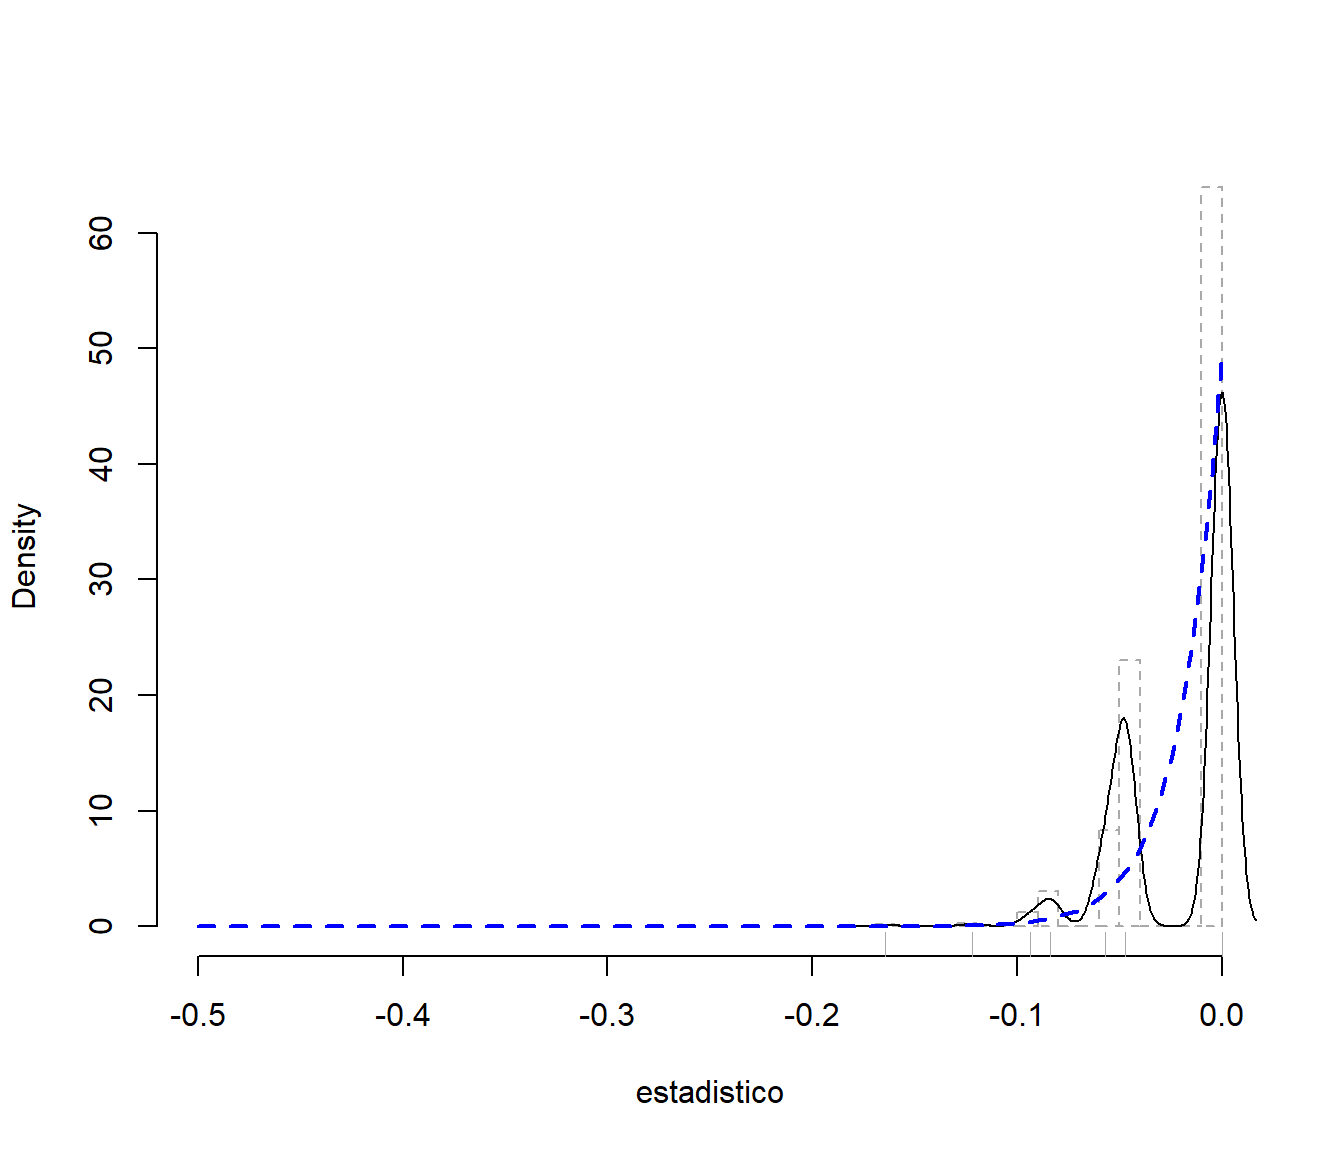
\includegraphics[width=0.7\linewidth]{04-mod_boot_unif_files/figure-latex/boot-uniforme-maximo-1} 

}

\caption{Distribución de las réplicas bootstrap (uniforme) del estadístico y distribución poblacional.}\label{fig:boot-uniforme-maximo}
\end{figure}

\subsection{Ejemplo (método
alternativo)}\label{ejemplo-metodo-alternativo}

En este contexto, al conocer la familia paramétrica
(\(\mathcal{U}\left( 0,\theta \right)\)) a la cual pertenece la
distribución de la población de partida, lo natural sería utilizar un
bootstrap paramétrico, consistente en obtener las remuestras bootstrap a
partir de una distribución uniforme con parámetro estimado:
\[\mathbf{X}^{\ast}=\left( X_1^{\ast}\text{, }X_2^{\ast}\text{, 
}\ldots \text{, }X_n^{\ast} \right), \text{ con } X_i^{\ast} \sim \mathcal{U}\left( 0,\hat{\theta}\right).\]
En estas circunstancias es muy sencillo obtener la distribución en el
remuestreo de \(\hat{\theta}^{\ast}\), ya que su deducción es totalmente
paralela a la de la distribución en el muestreo de \(\hat{\theta}\).
Así, la función de densidad de \(\hat{\theta}^{\ast}\) es
\[\hat{g}\left( x \right) =\frac{n}{\hat{\theta}}\left( \frac{x}{\hat{\theta}}
 \right)^{n-1},\text{ si }x\in \left[ 0,\hat{\theta}\right] .\]

Con lo cual, al utilizar un bootstrap paramétrico, la distribución en el
remuestreo de
\(R^{\ast}=R\left( \mathbf{X}^{\ast},F_{\hat{ \theta}} \right) =\hat{\theta}^{\ast}-\hat{\theta}\)
imita a la distribución en muestreo de
\(R=R\left( \mathbf{X},F \right) =\hat{\theta}-\theta\).

\BeginKnitrBlock{example}[Inferencia sobre el máximo de una distribución uniforme, continuación]
\protect\hypertarget{exm:boot-maximo-parametrico}{}{\label{exm:boot-maximo-parametrico}
\iffalse (Inferencia sobre el máximo de una distribución uniforme,
continuación) \fi{} }
\EndKnitrBlock{example}

Para emplear el bootstrap paramétrico (que remuestrea de una
distribución uniforme con parámetro estimado) podríamos emplear un
código muy similar al del Ejemplo \ref{exm:boot-maximo-uniforme}
{[}Figura \ref{fig:boot-parametrico-maximo}{]}:

\begin{Shaded}
\begin{Highlighting}[]
\CommentTok{# Remuestreo}
\NormalTok{B <-}\StringTok{ }\DecValTok{2000}
\NormalTok{maximo <-}\StringTok{ }\KeywordTok{numeric}\NormalTok{(B)}
\NormalTok{estadistico <-}\StringTok{ }\KeywordTok{numeric}\NormalTok{(B)}
\ControlFlowTok{for}\NormalTok{ (k }\ControlFlowTok{in} \DecValTok{1}\OperatorTok{:}\NormalTok{B) \{}
\NormalTok{    remuestra <-}\StringTok{ }\KeywordTok{runif}\NormalTok{(n) }\OperatorTok{*}\StringTok{ }\NormalTok{theta_est}
\NormalTok{    maximo[k] <-}\StringTok{ }\KeywordTok{max}\NormalTok{(remuestra)}
\NormalTok{    estadistico[k] <-}\StringTok{ }\NormalTok{maximo[k] }\OperatorTok{-}\StringTok{ }\NormalTok{theta_est}
\NormalTok{\}}
\CommentTok{# Distribución estadístico}
\NormalTok{xlim <-}\StringTok{ }\KeywordTok{c}\NormalTok{(}\OperatorTok{-}\NormalTok{theta}\OperatorTok{/}\DecValTok{2}\NormalTok{, }\DecValTok{0}\NormalTok{) }\CommentTok{# c(-theta, 0)}
\KeywordTok{hist}\NormalTok{(estadistico, }\DataTypeTok{freq =} \OtherTok{FALSE}\NormalTok{, }\DataTypeTok{main =} \StringTok{""}\NormalTok{, }\DataTypeTok{lty =} \DecValTok{2}\NormalTok{, }
     \DataTypeTok{border =} \StringTok{"darkgray"}\NormalTok{, }\DataTypeTok{xlim =}\NormalTok{ xlim)}
\KeywordTok{lines}\NormalTok{(}\KeywordTok{density}\NormalTok{(estadistico))}
\KeywordTok{rug}\NormalTok{(estadistico, }\DataTypeTok{col =} \StringTok{"darkgray"}\NormalTok{)}
\KeywordTok{curve}\NormalTok{(n}\OperatorTok{/}\NormalTok{theta }\OperatorTok{*}\StringTok{ }\NormalTok{((x }\OperatorTok{+}\StringTok{ }\NormalTok{theta)}\OperatorTok{/}\NormalTok{theta)}\OperatorTok{^}\NormalTok{(n }\OperatorTok{-}\StringTok{ }\DecValTok{1}\NormalTok{), }\DataTypeTok{col =} \StringTok{"blue"}\NormalTok{, }\DataTypeTok{lty =} \DecValTok{2}\NormalTok{, }\DataTypeTok{lwd =} \DecValTok{2}\NormalTok{, }\DataTypeTok{add =} \OtherTok{TRUE}\NormalTok{)}
\end{Highlighting}
\end{Shaded}

\begin{figure}[!htb]

{\centering 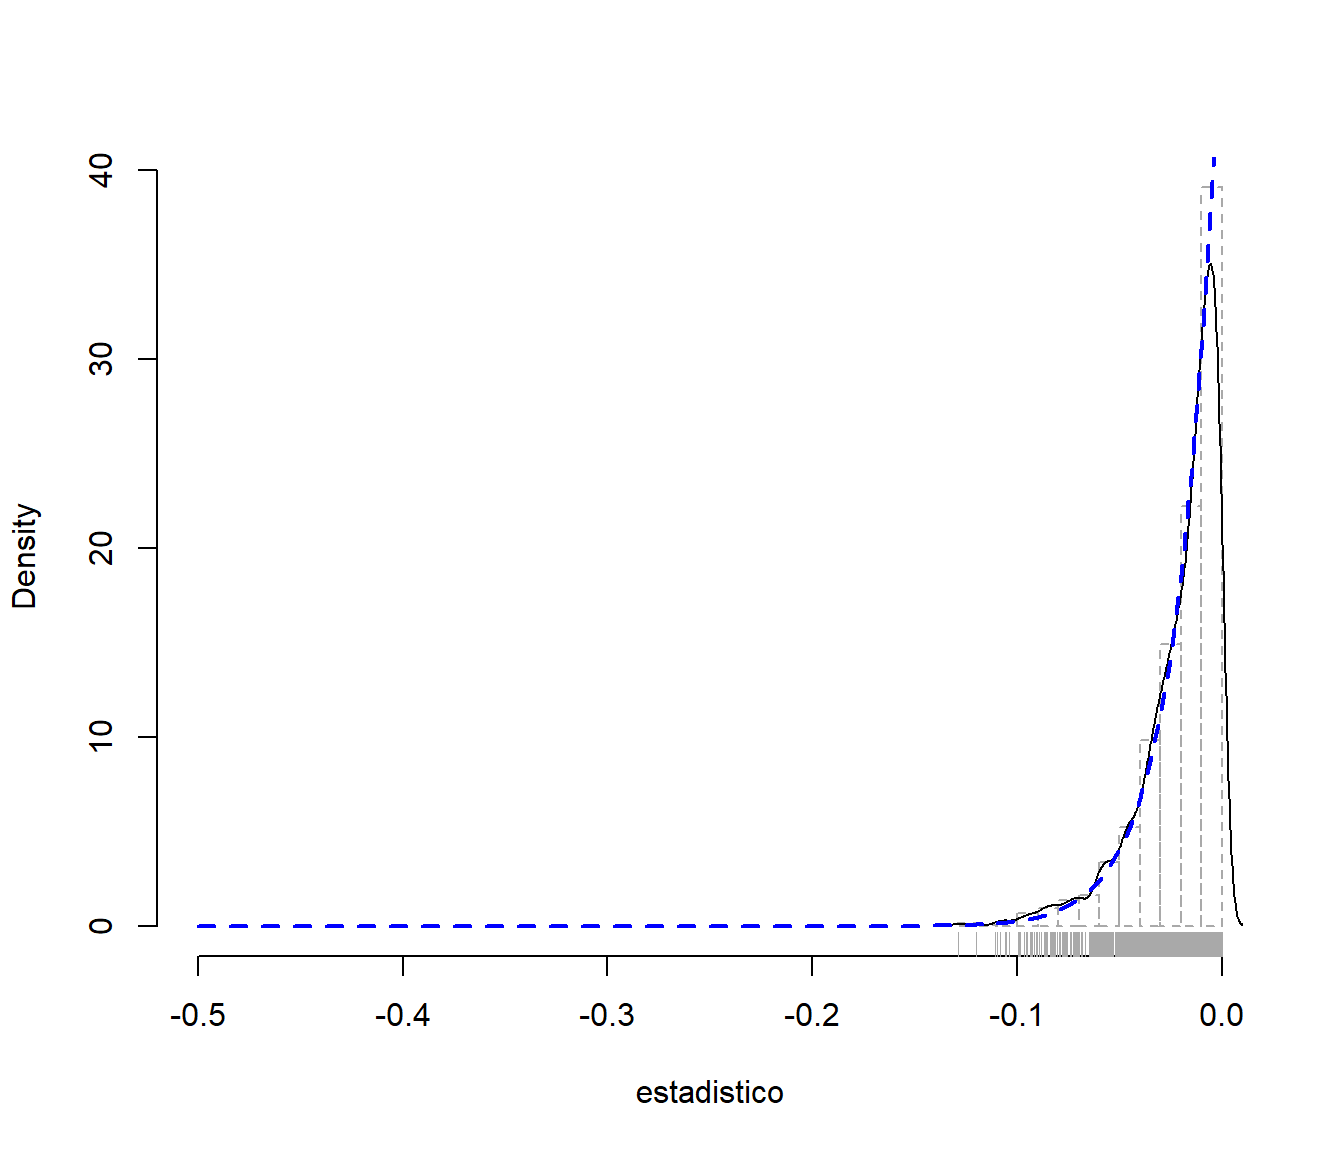
\includegraphics[width=0.7\linewidth]{04-mod_boot_unif_files/figure-latex/boot-parametrico-maximo-1} 

}

\caption{Distribución bootstrap paramétrica y distribución poblacional.}\label{fig:boot-parametrico-maximo}
\end{figure}

\section{Validez de la aproximación
Bootstrap}\label{validez-de-la-aproximacion-bootstrap}

Trataremos ahora de dar una justificación teórica del buen
funcionamiento del bootstrap uniforme. Para ello, por simplicidad, nos
centraremos en el problema de aproximar la distribución en el muestreo
del estadístico
\[R=R\left( \mathbf{X},F \right) =\sqrt{n}\frac{\bar{X}-\mu }{\sigma },\]
donde \(\mathbf{X}=\left( X_1,X_2,\ldots ,X_n \right)\) es una m.a.s.
procedente de una distribución \(F\), con media \(\mu\) y desviación
típica \(\sigma\). Sabemos que, bajo ciertas condiciones, el teorema
central del límite permite obtener la distribución asintótica de \(R\),
que es una \(\mathcal{N}\left( 0,1 \right)\), es decir
\[\lim_{n\rightarrow \infty }P\left( R\leq u \right) =\Phi \left( u \right),
\quad\forall u\in \mathbb{R},\] siendo \(\Phi\) la función de
distribución de una normal estándar, cuya función de densidad
denotaremos por \(\phi\).

Para ver cómo de buena es la aproximación por normal del estadístico
\(R\), debemos razonar cómo de rápida es la convergencia en el límite
anteriormente expuesto. La respuesta a esa pregunta viene dada por el
Teorema de Cramer que usa los llamados desarrollos de Edgeworth de un
estadístico para aproximarlo por una suma de términos, el primero es la
función de distribución normal estándar y los siguientes irán tendiendo
a cero sucesivamente más rápido cuando el tamaño muestral tiende a
infinito. Enunciemos ese resultado.

\BeginKnitrBlock{theorem}[Cramer]
\protect\hypertarget{thm:aprox-cramer}{}{\label{thm:aprox-cramer}
\iffalse (Cramer) \fi{} } \vspace{0.5cm}

Consideremos variables aleatorias \(X_1,X_2,\ldots ,X_n,\ldots\)
independientes e idénticamente distribuidas procedentes de una
distribución \(F\), con media \(\mu\) y desviación típica \(\sigma\).
Supongamos que existe cierto \(j\), natural, para el cual
\(E\left( \left\vert X\right\vert^{j+2} \right) <\infty \,\), y que
\(\lim_{\left\vert t\right\vert \rightarrow \infty }\left\vert \alpha \left( t \right) \right\vert <1\),
siendo \(\alpha \left( t \right) =E\left( e^{itX} \right)\) la función
característica de la población. Entonces: \[\begin{aligned}
P\left( R\leq u \right) &=P\left( \sqrt{n}\frac{\bar{X}-\mu }{\sigma }
\leq u \right) \\
&= \Phi \left( u \right) +n^{-\frac{1}{2}}p_1\left( u \right) \phi \left(
u \right) +\cdots +n^{-\frac{j-1}{2}}p_{j-1}\left( u \right) \phi \left(
u \right) +O\left( n^{-\frac{j}{2}} \right),
\end{aligned}\] siendo los \(p_i\left( u \right)\) polinomios de grado
\(3i-1\) cuyos coeficientes dependen de los momentos de \(X\) de orden
menor o igual que \(i+2\). En particular \[\begin{aligned}
p_1\left( u \right) &= -\frac{1}{6}\frac{k_3}{\sigma^{3}}\left(
u^2-1 \right), \\
p_2\left( u \right) &= -u\left[ \frac{1}{24}\frac{k_4}{\sigma^{4}}\left(
u^2-3 \right) +\frac{1}{72}\left( \frac{k_3}{\sigma^{3}} \right)
^2\left( u^{4}-10u^2+15 \right) \right] ,
\end{aligned}\]

siendo \(k_j\) el \(j\)-ésimo cumulante, es decir el términos que
acompaña a \(\frac{\left( it \right)^{j}}{j!}\) en el desarrollo en
serie del logaritmo de la función característica:
\[\log \alpha \left( t \right) =\sum_{j=1}^{\infty }k_j\frac{\left( it \right)
^{j}}{j!}.\]

Además dichos polinomios tienen paridad alternada, es decir, \(p_1\) es
simétrico, \(p_2\) es antisimétrico, \(p_3\) es simétrico, y así
sucesivamente:
\[p_1\left( -u \right) = p_1\left( u \right),\quad p_2\left( -u \right)
= -p_2\left( u \right),\quad p_3\left( -u \right) = p_3\left( u \right)
,\cdots\]
\EndKnitrBlock{theorem}

Existen ecuaciones que relacionan todos los cumulantes hasta cierto
orden con todos los momentos poblacionales hasta ese mismo orden. Dichas
ecuaciones permiten expresar los cumulantes en función de los momentos y
viceversa.

Como consecuencia de este resultado teórico, el grado de aproximación
entre la distribución de \(R\) y la normal estándar límite es
\(O (n^{-\frac{1}{2}})\). Sin embargo, puede razonarse fácilmente que
este orden de aproximación mejorará cuando utilizamos el bootstrap
uniforme, en lugar de la normal estándar, para aproximar la distribución
de \(R\). Un desarrollo de Edgeworth para la distribución en el
remuestreo de \(R^{\ast}\) permite obtener la siguiente expresión:
\[\begin{aligned}
P^{\ast}\left( R^{\ast}\leq u \right) &= \Phi \left( u \right) +n^{-\frac{1}{2}
}\hat{p}_1\left( u \right) \phi \left( u \right) +\cdots +n^{-\frac{j-1}{2}}
\hat{p}_{j-1}\left( u \right) \phi \left( u \right) \\
&+ O_{P}\left( n^{-\frac{j}{2}} \right),
\end{aligned}\]

donde los polinomios \(\hat{p}_i\left( u \right)\) tienen la misma
estructura que los \(p_i\left( u \right)\) pero reemplazando los
cumulantes teóricos por los empíricos y la desviación típica teórica por
la empírica. Así pues el grado de aproximación entre cada polinomio
\(\hat{p}_i( u )\) y su análogo teórico \(p_i( u )\) es
\(\hat{p}_i( u ) -p_i( u ) = O_{P}( n^{-\frac{1}{2}} )\). Como
consecuencia, puede obtenerse el orden de aproximación entre la
distribución en el muestreo de \(R\) y la distribución en el remuestreo
de \(R^{\ast}\): \[\begin{aligned}
P\left( R\leq u \right) -P^{\ast}\left( R^{\ast}\leq u \right) &=  n^{-\frac{1}{
2}}\left[ p_1\left( u \right) -\hat{p}_1\left( u \right) \right] \phi
\left( u \right) +O_{P}\left( n^{-1} \right) \\
&=  O_{P}\left( n^{-1} \right),\end{aligned}\]que es mejor que el orden
de aproximación de la normal estándar límite. Dichos órdenes pueden
resumirse en la siguiente tabla.

\begin{longtable}[]{@{}ll@{}}
\toprule
Aproximación & Orden\tabularnewline
\midrule
\endhead
Normal límite & \(O\left( n^{-\frac{1}{2}} \right)\)\tabularnewline
Boot. uniforme & \(O_{P}\left( n^{-1} \right)\)\tabularnewline
\bottomrule
\end{longtable}

Usando razonamiento similares pueden encontrarse los órdenes de
aproximación, tanto de la normal límite, como del bootstrap uniforme y
del bootstrap simetrizado, cuando la distribucional de partida es
simétrica. En ese caso, \(p_1\left( u \right) =0\), ya que \(k_3\) es
cero debido a la simetría de la distribución poblacional. Sin embargo
\(\hat{p}_1\left( u \right)\) no es cero cuando se usa el bootstrap
uniforme, aunque sí lo es en el caso del bootstrap simetrizado. La
siguiente tabla recoge los órdenes de las distintas aproximaciones.

\begin{longtable}[]{@{}ll@{}}
\toprule
Aproximación & Orden\tabularnewline
\midrule
\endhead
Normal límite & \(O\left( n^{-1} \right)\)\tabularnewline
Boot. uniforme & \(O_{P}\left( n^{-1} \right)\)\tabularnewline
Boot. simetrizado &
\(O_{P}\left( n^{-\frac{3}{2}} \right)\)\tabularnewline
\bottomrule
\end{longtable}

El siguiente resultado permite generalizar los desarrollos de Edgeworth
(Teorema \ref{thm:aprox-cramer}) a otros estadísticos (estandarizados o
studentizados) obtenidos para otros estimadores arbitrarios,
\(\hat{\theta}\), no necesariamente iguales a la media muestral.

\BeginKnitrBlock{theorem}[Bhattacharya-Ghosh]
\protect\hypertarget{thm:aprox-bhat-gho}{}{\label{thm:aprox-bhat-gho}
\iffalse (Bhattacharya-Ghosh) \fi{} } \vspace{0.5cm}

Consideremos variables aleatorias \(X_1,X_2,\ldots ,X_n,\ldots\)
independientes e idénticamente distribuidas procedentes de una
distribución \(F\). Sea \(\theta =\theta \left( F \right)\) un parámetro
de dicha distribución y \(\hat{\theta}\) un estimador de dicho
parámetro. Supongamos además
que\[\sqrt{n}\left( \hat{\theta}-\theta \right) \rightarrow \mathcal{N}\left( 0,\sigma
_{\theta }^2 \right),\] en distribución. Entonces, bajo ciertas
condiciones de regularidad (pueden verse en Bhattacharya y Ghosh, 1978)
se tiene: \[\begin{aligned}
P\left( \sqrt{n}\frac{\hat{\theta}-\theta }{\sigma _{\theta }}\leq u \right)
= &\ \Phi \left( u \right) +n^{-\frac{1}{2}}p_1\left( u \right) \phi \left(
u \right) +\cdots \\
& +n^{-\frac{j-1}{2}}p_{j-1}\left( u \right) \phi \left( u \right) +O\left(
n^{-\frac{j}{2}} \right), \\
P\left( \sqrt{n}\frac{\hat{\theta}-\theta }{\hat{\sigma}_{\theta }}\leq
u \right) = &\ \Phi \left( u \right) +n^{-\frac{1}{2}}q_1\left( u \right) \phi
\left( u \right) +\cdots \\
& +n^{-\frac{j-1}{2}}q_{j-1}\left( u \right) \phi \left( u \right) +O\left(
n^{-\frac{j}{2}} \right),\end{aligned}\]

siendo los \(p_i\left( u \right)\) y \(q_i\left( u \right)\) polinomios
de grado \(3i-1\) con paridad alternada, es decir, \(p_1\) y \(q_1\) son
simétricos, \(p_2\) y \(q_2\) son antisimétricos, \(p_3\) y \(q_3\) son
simétricos y así sucesivamente.
\EndKnitrBlock{theorem}

\chapter{Intervalos de confianza bootstrap}\label{cap5}

Consideremos el problema de construcción, mediante bootstrap, de un
intervalo de confianza bilateral, con nivel de confianza \(1-\alpha\),
para un parámetro \(\theta\) de la distribución \(F\). Una vez elegido
el método bootstrap adecuado a la información disponible en el contexto
del que se trate, un aspecto importante es el de la posible corrección
de los intervalos de confianza bootstrap, aproximados por el método de
Monte Carlo, al objeto de que la probabilidad de cobertura sea lo más
parecida posible al nivel nominal \(1-\alpha\). Comenzaremos analizando
el error de cobertura de los intervalos de confianza clásicos, los
basados en la distribución normal asintótica.

\section{Intervalos basados en la distribución normal
asintótica}\label{cap5_norm}

Consideremos primeramente el caso más sencillo (y poco realista) de
construcción de un intervalo de confianza para la media, \(\mu \,\), con
desviación típica, \(\sigma\), conocida. El estadístico usado para
construir el intervalo de confianza es
\[R=\sqrt{n}\frac{\bar{X}-\mu }{\sigma }\]que cuando
\(n\rightarrow \infty\) tiende en distribución a una
\(N\left( 0,1 \right)\). El intervalo de confianza basado en dicha
aproximación normal es
\(\hat{I}=\left( \bar{X}-\frac{\sigma }{\sqrt{n}}z_{\alpha /2}, \bar{X}+\frac{\sigma }{\sqrt{n}}z_{\alpha /2} \right)\).
Mediante el desarrollo de Edgeworth dado por el Teorema de Cramer es
fácil obtener una cota para el error de cobertura de dicho intervalo:

\[\begin{aligned}
P\left( \mu \in \hat{I} \right) -\left( 1-\alpha \right) =&\  P\left(
R<z_{\alpha /2} \right) -P\left( R\leq -z_{\alpha /2} \right) \\
&-\left( \Phi \left( z_{\alpha /2} \right) -\Phi \left( -z_{\alpha
/2} \right) \right) \\
=&\ \ n^{-\frac{1}{2}}p_1\left( z_{\alpha /2} \right) \phi \left( z_{\alpha
/2} \right) +O\left( n^{-1} \right) \\
&-\left( n^{-\frac{1}{2}}p_1\left( -z_{\alpha /2} \right) \phi \left(
-z_{\alpha /2} \right) +O\left( n^{-1} \right) \right) \\
=&\  O\left( n^{-1} \right),\end{aligned}\]

ya que por la simetría de las funciones \(p_1\left( u \right)\) y
\(\phi \left( u \right)\) se tiene
\[p_1\left( -z_{\alpha /2} \right) \phi \left( -z_{\alpha /2} \right)
=p_1\left( z_{\alpha /2} \right) \phi \left( z_{\alpha /2} \right).\] De
esta forma, el orden del error de cobertura del intervalo de confianza
bilateral con desviación típica poblacional conocida es
\(O\left( n^{-1} \right)\). Puede obtenerse fácilmente el orden del
error de cobertura de los intervalos unilaterales que resulta ser
\(O\left( n^{-\frac{1}{2}} \right)\).

En el caso más realista en que la desviación típica, \(\sigma\), sea
desconocida, el intervalo de confianza resulta \[\hat{I}_{0}=\left( 
\bar{X}-\frac{S_n}{\sqrt{n}}z_{\alpha /2},\bar{X}+\frac{S_n}{
\sqrt{n}}z_{\alpha /2} \right).\] Ahora, el estadístico en el que se
basa la inferencia resulta: \[R_1=\sqrt{n}\frac{\bar{X}-\mu }{S_n}.\] Un
desarrollo de Edgeworth del tipo del obtenido en el Teorema de
Bhattacharya-Ghosh permite acotar el error de cobertura de este
intervalo: \[\begin{aligned}
P\left( \mu \in \hat{I}_{0} \right) -\left( 1-\alpha \right) =&\ P\left(
R_1<z_{\alpha /2} \right) -P\left( R_1\leq -z_{\alpha /2} \right) \\
&-\left( \Phi \left( z_{\alpha /2} \right) -\Phi \left( -z_{\alpha
/2} \right) \right) \\
=&\ n^{-\frac{1}{2}}q_1\left( z_{\alpha /2} \right) \phi \left( z_{\alpha
/2} \right) +O\left( n^{-1} \right) \\
&-\left( n^{-\frac{1}{2}}q_1\left( -z_{\alpha /2} \right) \phi \left(
-z_{\alpha /2} \right) +O\left( n^{-1} \right) \right) \\
=&\ O\left( n^{-1} \right).
\end{aligned}\]

De esta forma, el orden del error de cobertura del intervalo de
confianza bilateral con desviación típica desconocida es
\(O\left( n^{-1} \right)\). El orden del error de cobertura para el
intervalo de confianza unilateral resulta
\(O\left( n^{-\frac{1}{2}} \right)\).

Si el parámetro de interés fuese otro arbitrario:
\(\theta =\theta \left( F \right)\), no necesariamente la media, puede
obtenerse, análogamente un intervalo de confianza basado en la normal
asintótica:
\[\hat{I}_{0}=\left( \hat{\theta}-\frac{\hat{\sigma}_{\theta }}{\sqrt{n}}
z_{\alpha /2},\hat{\theta}+\frac{\hat{\sigma}_{\theta }}{\sqrt{n}}
z_{\alpha/2} \right),\] que está basado en el estadístico
\[R_1=\sqrt{n}\frac{\hat{\theta}-\theta }{\hat{\sigma}_{\theta }}.\] De
forma análoga a lo ya razonado para la media muestral, puede deducirse
que el error de cobertura del intervalo de confianza bilateral tiene un
orden de \(O\left( n^{-1} \right)\), mientras que para intervalos
unilaterales el orden es \(O\left( n^{-\frac{1}{2}} \right)\).

\section{Método percentil (básico)}\label{cap5_basic}

Este método se basa en la construcción del intervalo de confianza,
mediante bootstrap, a partir del estadístico no estandarizado
\[R_2=\sqrt{n}\left( \hat{\theta}-\theta \right).\] Una vez realizado el
correspondiente remuestreo (uniforme, suavizado, simetrizado, \ldots{}),
a partir de cierto estimador, \(\hat{F}\,\), de la distribución
poblacional, \(F\), la distribución en el muestreo de \(R_2\) se
aproxima mediante la distribución bootstrap de
\[R_2^{\ast}=\sqrt{n}\left( \hat{\theta}^{\ast}-\theta \left( \hat{F}
 \right) \right).\] Así se obtienen valores \(x_{\alpha /2}\) y
\(x_{1-\alpha /2}\), siendo \(x_{\beta }\), tal que
\(P^{\ast}\left( R_2^{\ast }\leq x_{\beta } \right) =\beta\), y a partir
de ellos sabemos que \[\begin{aligned}
1-\alpha &= 1-\frac{\alpha }{2}-\frac{\alpha }{2}=P^{\ast}\left(
R_2^{\ast}<x_{1-\alpha /2} \right) -P^{\ast}\left( R_2^{\ast}\leq
x_{\alpha /2} \right) \\
&= P^{\ast}\left( x_{\alpha /2}<R_2^{\ast}<x_{1-\alpha /2} \right),
\end{aligned}\] con lo cual decimos que también ha de ser
aproximadamente igual a \(1-\alpha\) la siguiente
probabilidad\[\begin{aligned}
P\left( x_{\alpha /2}<R_2<x_{1-\alpha /2} \right) &= P\left( x_{\alpha /2}<
\sqrt{n}\left( \hat{\theta}-\theta \right) <x_{1-\alpha /2} \right) \\
&= P\left( \hat{\theta}-\frac{x_{1-\alpha /2}}{\sqrt{n}}<\theta <\hat{\theta}
-\frac{x_{\alpha /2}}{\sqrt{n}} \right).\end{aligned}\] Ello da pie a
definir el intervalo de confianza bootstrap calculado por el método
percentil como
\[\hat{I}_1=\left( \hat{\theta}-\frac{x_{1-\alpha /2}}{\sqrt{n}},\hat{\theta}
-\frac{x_{\alpha /2}}{\sqrt{n}} \right).\]

Para estudiar el error de cobertura de este intervalo de confianza
conviene ver antes qué grado de aproximación existe entre la
distribución en el muestreo de \(R_2\) y la distribución bootstrap de
\(R_2^{\ast}\). A partir del Teorema de Bhattacharya-Ghosh se
tiene\[\begin{aligned}
P\left( R_2\leq v \right) &= P\left( \sqrt{n}\left( \hat{\theta}-\theta
 \right) \leq v \right) =P\left( \sqrt{n}\frac{\hat{\theta}-\theta }{\sigma
_{\theta }}\leq \frac{v}{\sigma _{\theta }} \right) \\
&= \Phi \left( \frac{v}{\sigma _{\theta }} \right) +O\left( n^{-\frac{1}{2}
} \right) \\
P^{\ast}\left( R_2^{\ast}\leq v \right) &= P^{\ast}\left( \sqrt{n}\left( 
\hat{\theta}^{\ast}-\theta \left( \hat{F} \right) \right) \leq v \right)
\\
&=  P^{\ast}\left( \sqrt{n}\frac{\hat{\theta}^{\ast}-\theta \left( \hat{F}
 \right)}{\sigma _{\hat{\theta}}}\leq \frac{v}{\sigma _{\hat{\theta}}} \right)
=\Phi \left( \frac{v}{\sigma _{\hat{\theta}}} \right) +O_{P}\left( n^{-
\frac{1}{2}} \right).
\end{aligned}\]

Como consecuencia
\[P^{\ast}\left( R_2^{\ast}\leq v \right) -P\left( R_2\leq v \right) =\Phi
\left( \frac{v}{\sigma _{\hat{\theta}}} \right) -\Phi \left( \frac{v}{\sigma
_{\theta }} \right) +O_{P}\left( n^{-\frac{1}{2}} \right) =O_{P}\left( n^{-
\frac{1}{2}} \right),\] ya que, típicamente,
\(\sigma _{\hat{\theta}}-\sigma _{\theta} = O_{P}\left( n^{-\frac{1}{2}} \right)\).
En resumen, la distribución en el muestreo de \(R_2\) y la distribución
bootstrap de \(R_2^{\ast}\) se aproximan, una a la otra, a la velocidad
\(O_{P}\left( n^{-\frac{1}{2} } \right)\), cuando
\(n\rightarrow \infty\).

El error de cobertura del intervalo de confianza bilateral calculado
mediante bootstrap por el método percentil es \[\begin{aligned}
P\left( \theta \in \hat{I}_1 \right) -\left( 1-\alpha \right) =&\ P\left(
R_2<x_{1-\alpha /2} \right) -P\left( R_2\leq x_{\alpha /2} \right) \\
&-\left[ P^{\ast}\left( R_2^{\ast}<x_{1-\alpha /2} \right) -P^{\ast
}\left( R_2^{\ast}\leq x_{\alpha /2} \right) \right] \\
=&\ P\left( R_2<x_{1-\alpha /2} \right) -P^{\ast}\left( R_2^{\ast
}<x_{1-\alpha /2} \right) \\
&-\left[ P\left( R_2\leq x_{\alpha /2} \right) -P^{\ast}\left(
R_2^{\ast}\leq x_{\alpha /2} \right) \right] \\
=&\ O_{P}\left( n^{-\frac{1}{2}} \right)
\end{aligned}\]

De esta forma el error de cobertura para los intervalos de confianza
bilaterales bootstrap obtenidos mediante el método percentil es
\(O\left( n^{-\frac{1}{2}} \right)\). Puede deducirse que ese es también
el orden para los intervalos unilaterales obtenidos por este método. Así
pues el orden del error de cobertura para el método percentil cuando se
construyen intervalos de confianza unilaterales coincide con el de los
construidos usando la normal asintótica pero el orden del error de
cobertura de los intervalos bilaterales bootstrap constuidos por el
método percentil es peor que el de los basados en la normal asintótica,
que es del orden \(O\left( n^{-1} \right)\).

\BeginKnitrBlock{example}[Inferencia sobre la media con varianza desconocida, continuación]
\protect\hypertarget{exm:media-dt-desconocida-perc}{}{\label{exm:media-dt-desconocida-perc}
\iffalse (Inferencia sobre la media con varianza desconocida,
continuación) \fi{} } \vspace{0.5cm}

Continuando con el ejemplo de los tiempos de vida de microorganismos
(sin asumir varianza conocida), supongamos que queremos obtener una
estimación por intervalo de confianza de su vida media empleando este
método. El código necesario sería muy similar al del Ejemplo
\ref{exm:media-dt-desconocida}:
\EndKnitrBlock{example}

\begin{Shaded}
\begin{Highlighting}[]
\NormalTok{muestra <-}\StringTok{ }\KeywordTok{c}\NormalTok{(}\FloatTok{0.143}\NormalTok{, }\FloatTok{0.182}\NormalTok{, }\FloatTok{0.256}\NormalTok{, }\FloatTok{0.26}\NormalTok{, }\FloatTok{0.27}\NormalTok{, }\FloatTok{0.437}\NormalTok{, }\FloatTok{0.509}\NormalTok{, }
             \FloatTok{0.611}\NormalTok{, }\FloatTok{0.712}\NormalTok{, }\FloatTok{1.04}\NormalTok{, }\FloatTok{1.09}\NormalTok{, }\FloatTok{1.15}\NormalTok{, }\FloatTok{1.46}\NormalTok{, }\FloatTok{1.88}\NormalTok{, }\FloatTok{2.08}\NormalTok{)}
\NormalTok{n <-}\StringTok{ }\KeywordTok{length}\NormalTok{(muestra)}
\NormalTok{alfa <-}\StringTok{ }\FloatTok{0.05}
\NormalTok{x_barra <-}\StringTok{ }\KeywordTok{mean}\NormalTok{(muestra)}

\CommentTok{# Remuestreo}
\KeywordTok{set.seed}\NormalTok{(}\DecValTok{1}\NormalTok{)}
\NormalTok{B <-}\StringTok{ }\DecValTok{1000}
\NormalTok{remuestra <-}\StringTok{ }\KeywordTok{numeric}\NormalTok{(n)}
\NormalTok{x_barra_boot <-}\StringTok{ }\KeywordTok{numeric}\NormalTok{(B) }
\NormalTok{estadistico_boot <-}\StringTok{ }\KeywordTok{numeric}\NormalTok{(B)}
\ControlFlowTok{for}\NormalTok{ (k }\ControlFlowTok{in} \DecValTok{1}\OperatorTok{:}\NormalTok{B) \{}
\NormalTok{  remuestra <-}\StringTok{ }\KeywordTok{sample}\NormalTok{(muestra, n, }\DataTypeTok{replace =} \OtherTok{TRUE}\NormalTok{)}
\NormalTok{  x_barra_boot[k] <-}\StringTok{ }\KeywordTok{mean}\NormalTok{(remuestra)}
\NormalTok{  estadistico_boot[k] <-}\StringTok{ }\KeywordTok{sqrt}\NormalTok{(n) }\OperatorTok{*}\StringTok{ }\NormalTok{(x_barra_boot[k] }\OperatorTok{-}\StringTok{ }\NormalTok{x_barra)}
\NormalTok{\}}

\CommentTok{# Aproximación bootstrap de los ptos críticos}
\NormalTok{pto_crit <-}\StringTok{ }\KeywordTok{quantile}\NormalTok{(estadistico_boot, }\KeywordTok{c}\NormalTok{(alfa}\OperatorTok{/}\DecValTok{2}\NormalTok{, }\DecValTok{1} \OperatorTok{-}\StringTok{ }\NormalTok{alfa}\OperatorTok{/}\DecValTok{2}\NormalTok{))}

\CommentTok{# Construcción del IC}
\NormalTok{ic_inf_boot <-}\StringTok{ }\NormalTok{x_barra }\OperatorTok{-}\StringTok{ }\NormalTok{pto_crit[}\DecValTok{2}\NormalTok{]}\OperatorTok{/}\KeywordTok{sqrt}\NormalTok{(n)}
\NormalTok{ic_sup_boot <-}\StringTok{ }\NormalTok{x_barra }\OperatorTok{-}\StringTok{ }\NormalTok{pto_crit[}\DecValTok{1}\NormalTok{]}\OperatorTok{/}\KeywordTok{sqrt}\NormalTok{(n)}
\NormalTok{IC_boot <-}\StringTok{ }\KeywordTok{c}\NormalTok{(ic_inf_boot, ic_sup_boot)}
\KeywordTok{names}\NormalTok{(IC_boot) <-}\StringTok{ }\KeywordTok{paste0}\NormalTok{(}\DecValTok{100}\OperatorTok{*}\KeywordTok{c}\NormalTok{(alfa}\OperatorTok{/}\DecValTok{2}\NormalTok{, }\DecValTok{1}\OperatorTok{-}\NormalTok{alfa}\OperatorTok{/}\DecValTok{2}\NormalTok{), }\StringTok{"%"}\NormalTok{)}
\NormalTok{IC_boot}
\end{Highlighting}
\end{Shaded}

\begin{verbatim}
##     2.5%    97.5% 
## 0.457700 1.092293
\end{verbatim}

Aunque en este caso también podemos obtener el intervalo a partir de las
réplicas bootstrap del estimador:

\begin{Shaded}
\begin{Highlighting}[]
\NormalTok{pto_crit <-}\StringTok{ }\KeywordTok{quantile}\NormalTok{(x_barra_boot, }\KeywordTok{c}\NormalTok{(alfa}\OperatorTok{/}\DecValTok{2}\NormalTok{, }\DecValTok{1} \OperatorTok{-}\StringTok{ }\NormalTok{alfa}\OperatorTok{/}\DecValTok{2}\NormalTok{))}
\NormalTok{ic_inf_boot <-}\StringTok{ }\DecValTok{2}\OperatorTok{*}\NormalTok{x_barra }\OperatorTok{-}\StringTok{ }\NormalTok{pto_crit[}\DecValTok{2}\NormalTok{]}
\NormalTok{ic_sup_boot <-}\StringTok{ }\DecValTok{2}\OperatorTok{*}\NormalTok{x_barra }\OperatorTok{-}\StringTok{ }\NormalTok{pto_crit[}\DecValTok{1}\NormalTok{]}
\NormalTok{IC_boot <-}\StringTok{ }\KeywordTok{c}\NormalTok{(ic_inf_boot, ic_sup_boot)}
\KeywordTok{names}\NormalTok{(IC_boot) <-}\StringTok{ }\KeywordTok{paste0}\NormalTok{(}\DecValTok{100}\OperatorTok{*}\KeywordTok{c}\NormalTok{(alfa}\OperatorTok{/}\DecValTok{2}\NormalTok{, }\DecValTok{1}\OperatorTok{-}\NormalTok{alfa}\OperatorTok{/}\DecValTok{2}\NormalTok{), }\StringTok{"%"}\NormalTok{)}
\NormalTok{IC_boot}
\end{Highlighting}
\end{Shaded}

\begin{verbatim}
##     2.5%    97.5% 
## 0.457700 1.092293
\end{verbatim}

Esta forma de proceder es la que emplea el paquete \texttt{boot} para
obtener el que denomina intervalo de confianza \emph{bootstrap básico}
(estableciendo \texttt{type="basic"} en la llamada a la función
\texttt{boot.ci()}):

\begin{Shaded}
\begin{Highlighting}[]
\KeywordTok{library}\NormalTok{(boot)}
\NormalTok{statistic <-}\StringTok{ }\ControlFlowTok{function}\NormalTok{(data, i) }\KeywordTok{mean}\NormalTok{(data[i])}

\KeywordTok{set.seed}\NormalTok{(}\DecValTok{1}\NormalTok{)}
\NormalTok{res.boot <-}\StringTok{ }\KeywordTok{boot}\NormalTok{(muestra, statistic, }\DataTypeTok{R =} \DecValTok{1000}\NormalTok{)}
\NormalTok{res <-}\StringTok{ }\KeywordTok{boot.ci}\NormalTok{(res.boot, }\DataTypeTok{type =} \StringTok{"basic"}\NormalTok{)}
\NormalTok{res}
\end{Highlighting}
\end{Shaded}

\begin{verbatim}
## BOOTSTRAP CONFIDENCE INTERVAL CALCULATIONS
## Based on 1000 bootstrap replicates
## 
## CALL : 
## boot.ci(boot.out = res.boot, type = "basic")
## 
## Intervals : 
## Level      Basic         
## 95%   ( 0.4945,  1.1121 )  
## Calculations and Intervals on Original Scale
\end{verbatim}

\begin{Shaded}
\begin{Highlighting}[]
\NormalTok{IC_boot <-}\StringTok{ }\NormalTok{res}\OperatorTok{$}\NormalTok{basic[}\DecValTok{4}\OperatorTok{:}\DecValTok{5}\NormalTok{]}
\NormalTok{IC_boot}
\end{Highlighting}
\end{Shaded}

\begin{verbatim}
## [1] 0.494535 1.112066
\end{verbatim}

Además del paquete \texttt{boot}, otros autores también denominan a este
método \emph{bootstrap básico} (\emph{bootstrap percentil básico} o
incluso \emph{bootstrap natural}), y utilizan la terminología
\emph{bootstrap percentil} cuando se emplea directamente el estimador
como estadístico (\(R = \hat \theta\)) para realizar inferencia. Con el
paquete \texttt{boot} habrá que establecer \texttt{type="perc"} en la
llamada a la función \texttt{boot.ci()} para obtener el intervalo
correspondiente:

\begin{Shaded}
\begin{Highlighting}[]
\KeywordTok{boot.ci}\NormalTok{(res.boot, }\DataTypeTok{type =} \StringTok{"perc"}\NormalTok{)}
\end{Highlighting}
\end{Shaded}

\begin{verbatim}
## BOOTSTRAP CONFIDENCE INTERVAL CALCULATIONS
## Based on 1000 bootstrap replicates
## 
## CALL : 
## boot.ci(boot.out = res.boot, type = "perc")
## 
## Intervals : 
## Level     Percentile     
## 95%   ( 0.4986,  1.1161 )  
## Calculations and Intervals on Original Scale
\end{verbatim}

En este método se emplean directamente los cuantiles de las réplicas
bootstrap del estadístico:

\begin{Shaded}
\begin{Highlighting}[]
\CommentTok{# IC_boot <-  quantile(res.boot$t, c(alfa/2, 1 - alfa/2)) # type = 7}
\NormalTok{IC_boot <-}\StringTok{  }\KeywordTok{quantile}\NormalTok{(res.boot}\OperatorTok{$}\NormalTok{t, }\KeywordTok{c}\NormalTok{(alfa}\OperatorTok{/}\DecValTok{2}\NormalTok{, }\DecValTok{1} \OperatorTok{-}\StringTok{ }\NormalTok{alfa}\OperatorTok{/}\DecValTok{2}\NormalTok{), }\DataTypeTok{type =} \DecValTok{6}\NormalTok{)}
\NormalTok{IC_boot }
\end{Highlighting}
\end{Shaded}

\begin{verbatim}
##      2.5%     97.5% 
## 0.4985983 1.1161317
\end{verbatim}

Asintóticamente ambos métodos son equivalentes, aunque en general es
preferible (evita sesgos) el bootstrap percentil básico.

\section{\texorpdfstring{Método
percentil-\emph{t}}{Método percentil-t}}\label{cap5-perc-t}

Este método bootstrap, construye un intervalo de confianza bootstrap a
partir del estadístico studentizado:
\[R_1=\sqrt{n}\frac{\hat{\theta}-\theta }{\hat{\sigma}_{\theta }}.\] Su
distribución en el muestreo se aproxima mediante la distribución
bootstrap de
\[R_1^{\ast}=\sqrt{n}\frac{\hat{\theta}^{\ast}-\theta \left( \hat{F}
 \right)}{\hat{\sigma}_{\theta }^{\ast}}.\] En este caso, los valores
\(x_{\alpha /2}\) y \(x_{1-\alpha /2}\), se obtienen a partir de esta
última distribución bootstrap, es decir, \(x_{\beta }\) se define a
partir de \(P^{\ast}\left( R_1^{\ast}\leq x_{\beta } \right) =\beta\).
Como
\[1-\alpha =P^{\ast}\left( x_{\alpha /2}<R_1^{\ast}<x_{1-\alpha /2} \right),\]
razonamos que también ha de ser aproximadamente igual a \(1-\alpha\) la
siguiente probabilidad \[\begin{aligned}
P\left( x_{\alpha /2}<R_1<x_{1-\alpha /2} \right) &= P\left( x_{\alpha /2}<
\sqrt{n}\frac{\hat{\theta}-\theta }{\hat{\sigma}_{\theta }}<x_{1-\alpha
/2} \right) \\
&= P\left( \hat{\theta}-\frac{\hat{\sigma}_{\theta }}{\sqrt{n}}x_{1-\alpha
/2}<\theta <\hat{\theta}-\frac{\hat{\sigma}_{\theta }}{\sqrt{n}}x_{\alpha
/2} \right).
\end{aligned}\] Con lo cual, el intervalo de confianza bootstrap
calculado por el método percentil-\(t\) se define como
\[\hat{I}_2=\left( \hat{\theta}-\frac{\hat{\sigma}_{\theta }}{\sqrt{n}}
x_{1-\alpha /2},\hat{\theta}-\frac{\hat{\sigma}_{\theta }}{\sqrt{n}}
x_{\alpha /2} \right).\]

Utilizando el Teorema de Bhattacharya-Ghosh puede acotarse el error de
aproximación entre la distribución en el muestreo de \(R_1\) y la
distribución bootstrap de \(R_1^{\ast}\): \[\begin{aligned}
P^{\ast}\left( R_1^{\ast}\leq u \right) -P\left( R_1\leq u \right)
=&\ P^{\ast}\left( \sqrt{n}\frac{\hat{\theta}^{\ast}-\theta \left( \hat{F}
 \right)}{\hat{\sigma}_{\theta }^{\ast}}\leq u \right)-P\left( \sqrt{n}
\frac{\hat{\theta}-\theta }{\hat{\sigma}_{\theta }}\leq u \right)  \\
=&\  \Phi \left( u \right) +n^{-\frac{1}{2}}\hat{q}_1\left( u \right) \phi
\left( u \right) +O_{P}\left( n^{-1} \right) \\
&-\left[ \Phi \left( u \right) +n^{-\frac{1}{2}}q_1\left( u \right) \phi
\left( u \right) +O\left( n^{-1} \right) \right] \\
=&\  n^{-\frac{1}{2}}\left[ \hat{q}_1\left( u \right) -q_1\left( u \right) 
\right] \phi \left( u \right) +O_{P}\left( n^{-1} \right) \\
=&\ O_{P}\left( n^{-1} \right),
\end{aligned}\] ya que los coeficientes que aparecen en el polinomio
\(\hat{q}_1\left( u \right)\) son estimadores \(\sqrt{n}\)-consistentes
de los coeficientes del polinomio \(q_1\left( u \right)\). Los de éste
último dependen de los momentos poblacionales y los del primero son sus
correspondientes versiones empíricas.

Así pues, el error de cobertura del intervalo de confianza bootstrap
bilateral calculado por el método percentil-\(t\) es \[\begin{aligned}
P\left( \theta \in \hat{I}_2 \right) -\left( 1-\alpha \right) =&\  P\left(
R_1<x_{1-\alpha /2} \right) -P\left( R_1\leq x_{\alpha /2} \right) \\
& -\left[ P^{\ast}\left( R_1^{\ast}<x_{1-\alpha /2} \right) -P^{\ast
}\left( R_1^{\ast}\leq x_{\alpha /2} \right) \right] \\
=&\  P\left( R_1<x_{1-\alpha /2} \right) -P^{\ast}\left( R_1^{\ast
}<x_{1-\alpha /2} \right) \\
&-\left[ P\left( R_1\leq x_{\alpha /2} \right) -P^{\ast}\left(
R_1^{\ast}\leq x_{\alpha /2} \right) \right] \\
=&\  O_{P}\left( n^{-1} \right)
\end{aligned}\]

Se tiene entonces que el error de cobertura para los intervalos de
confianza bilaterales bootstrap obtenidos mediante el método
percentil-\(t\) es \(O\left( n^{-1} \right)\). Puede deducirse que ese
es también el orden para los intervalos unilaterales obtenidos por este
método. Así pues el orden del error de cobertura para el método
percentil-\(t\) cuando se construyen intervalos de confianza
unilaterales mejora al de los intervalos unilaterales basados en la
normal asintótica, con un error de cobertura de orden
\(O\left( n^{-\frac{1}{2}} \right)\). En el caso de los intervalos de
confianza bilaterales, el orden del error de cobertura usando la normal
asintótica o bien el bootstrap por el método percentil-\(t\) es el
mismo, \(O\left( n^{-1} \right)\) en ambos casos.

En el Ejemplo \ref{exm:media-dt-desconocida}, se implementó este método
para obtener una estimación por intervalo de confianza del tiempo de
vida medio de microorganismos. En el Ejemplo
\ref{exm:media-dt-desconocida-boot} se mostró como calcular este
intervalo empleando el paquete \texttt{boot} (haciendo que la función
\texttt{statistic} devuelva también la varianza del estadístico y
estableciendo \texttt{type="stud"} en la llamada a la función
\texttt{boot.ci()}).

\section{\texorpdfstring{Método percentil-\emph{t}
simetrizado}{Método percentil-t simetrizado}}\label{cap5-perc-t-sim}

Es un método análogo al percentil-\(t\). Sólo difiere de él en la forma
de seleccionar los cuantiles de la distribución bootstrap. En lugar de
tomar cuantiles que dejen colas iguales (\(\frac{\alpha }{2}\) a la
izquierda y a la derecha, respectivamente), se eligen los cuantiles de
forma que sean simétricos. Así, dado el estadístico \(R_1\) y su versión
bootstrap \(R_1^{\ast}\), se considera el valor \(y_{1-\alpha }\) que
cumple
\(P^{\ast}\left( \left\vert R_1^{\ast}\right\vert \leq y_{1-\alpha } \right) =1-\alpha\).
Así se tiene que
\[1-\alpha =P^{\ast}\left( -y_{1-\alpha }\leq R_1^{\ast}
\leq y_{1-\alpha} \right).\] De esa forma se razona que también ha de
ser aproximadamente igual a \(1-\alpha\) la siguiente probabilidad
\[\begin{aligned}
P\left( -y_{1-\alpha }<R_1<y_{1-\alpha } \right) &= P\left( -y_{1-\alpha }
< \sqrt{n}\frac{\hat{\theta}-\theta }{\hat{\sigma}_{\theta }}
< y_{1-\alpha} \right) \\
&= P\left( \hat{\theta}-\frac{\hat{\sigma}_{\theta }}{\sqrt{n}}y_{1-\alpha
}<\theta <\hat{\theta}+\frac{\hat{\sigma}_{\theta }}{\sqrt{n}}y_{1-\alpha
} \right).
\end{aligned}\]

Con lo cual, el intervalo de confianza bootstrap calculado por el método
percentil-\(t\) simetrizado se define como
\[\hat{I}_3=\left( \hat{\theta}-\frac{\hat{\sigma}_{\theta }}{\sqrt{n}}
y_{1-\alpha },\hat{\theta}+\frac{\hat{\sigma}_{\theta }}{\sqrt{n}}
y_{1-\alpha } \right).\]

Utilizando el Teorema de Bhattacharya-Ghosh con desarrollos hasta el
orden \(n^{-1}\) se tiene: \[\begin{aligned}
P^{\ast}\left( R_1^{\ast}\leq u \right) -P\left( R_1\leq u \right) 
=&\ P^{\ast}\left( \sqrt{n}\frac{\hat{\theta}^{\ast}-\theta \left( \hat{F}
 \right)}{\hat{\sigma}_{\theta }^{\ast}}\leq u \right) -P\left( \sqrt{n}
\frac{\hat{\theta}-\theta }{\hat{\sigma}_{\theta }}\leq u \right) \\
=&\ \Phi \left( u \right) +n^{-\frac{1}{2}}\hat{q}_1\left( u \right) \phi
\left( u \right) +n^{-1}\hat{q}_2\left( u \right) \phi \left( u \right)
+O_{P}\left( n^{-\frac{3}{2}} \right) \\
& -\left[ \Phi \left( u \right) +n^{-\frac{1}{2}}q_1\left( u \right) \phi
\left( u \right) +n^{-1}q_2\left( u \right) \phi \left( u \right) +O\left(
n^{-\frac{3}{2}} \right) \right] \\
=&\ n^{-\frac{1}{2}}\left[ \hat{q}_1\left( u \right) -q_1\left( u \right) 
\right] \phi \left( u \right) 
+n^{-1}\left[ \hat{q}_2\left( u \right) -q_2\left( u \right) \right] \phi
\left( u \right) +O_{P}\left( n^{-\frac{3}{2}} \right).
\end{aligned}\]

Como consecuencia, el error de cobertura del intervalo de confianza
bootstrap bilateral calculado por el método percentil-\(t\) simetrizado
es \[\begin{aligned}
P\left( \theta \in \hat{I}_3 \right) -\left( 1-\alpha \right) 
=&\ P\left(-y_{1-\alpha }<R_1<y_{1-\alpha } \right) -P^{\ast}\left( -y_{1-\alpha
}<R_1^{\ast}<y_{1-\alpha } \right) \\
=&\ P\left( R_1<y_{1-\alpha } \right) -P^{\ast}\left( R_1^{\ast
}<y_{1-\alpha } \right) - \\
&-\left[ P\left( R_1\leq -y_{1-\alpha } \right) -P^{\ast}\left( R_1^{\ast
}\leq -y_{1-\alpha } \right) \right] \\
=&\ n^{-\frac{1}{2}}\left[ q_1\left( y_{1-\alpha } \right) -\hat{q}_1\left(
y_{1-\alpha } \right) \right] \phi \left( y_{1-\alpha } \right) \\
&+n^{-1}\left[ q_2\left( y_{1-\alpha } \right) -\hat{q}_2\left(
y_{1-\alpha } \right) \right] \phi \left( y_{1-\alpha } \right) \\
&-n^{-\frac{1}{2}}\left[ q_1\left( -y_{1-\alpha } \right) -\hat{q}_1\left(
-y_{1-\alpha } \right) \right] \phi \left( -y_{1-\alpha } \right) \\
&-n^{-1}\left[ q_2\left( -y_{1-\alpha } \right) -\hat{q}_2\left(
-y_{1-\alpha } \right) \right] \phi \left( -y_{1-\alpha } \right) +O_{P}\left(
n^{-\frac{3}{2}} \right) \\
=&\ 2n^{-1}\left[ q_2\left( y_{1-\alpha } \right) -\hat{q}_2\left(
y_{1-\alpha } \right) \right] \phi \left( y_{1-\alpha } \right) +O_{P}\left(
n^{-\frac{3}{2}} \right) \\
=&\ O_{P}\left( n^{-\frac{3}{2}} \right)
\end{aligned}\]

ya que los polinomios \(q_1\left( u \right)\) y
\(\hat{q}_1\left( u \right)\) son simétricos, \(q_2\left( u \right)\) y
\(\hat{q}_2\left( u \right)\) son antisimétricos, la función
\(\phi \left( u \right)\) es simétrica y los coeficientes que aparecen
en el polinomio \(\hat{q}_2\left( u \right)\) son estimadores
\(\sqrt{n}\)-consistentes de los coeficientes del polinomio
\(q_2\left( u \right)\). Como consecuencia, el error de cobertura para
los intervalos de confianza bilaterales bootstrap obtenidos mediante el
método percentil-\(t\) simetrizado es
\(O\left( n^{-\frac{3}{2}} \right)\). Puede deducirse que el orden para
los intervalos unilaterales obtenidos por este método es
\(O\left( n^{-1} \right)\). Así pues el orden del error de cobertura
para el método percentil-\(t\) simetrizado cuando se construyen
intervalos de confianza unilaterales mejora al de los intervalos
unilaterales basados en la normal asintótica, con un error de cobertura
de orden \(O\left( n^{-\frac{1}{2}} \right)\), e iguala al orden del
error de cobertura de los obtenidos mediante el percentil-\(t\). En el
caso de los intervalos de confianza bilaterales, el orden del error de
cobertura usando el método percentil-\(t\) simetrizado es
\(O\left( n^{-\frac{3}{2}} \right)\), el cual mejora el orden
\(O\left( n^{-1} \right)\), que es el que presentan los intervalos
basados en la normal asintótica o bien en el método percentil-\(t\).

\section{Tabla resumen de los errores de
cobertura}\label{cap5_err_cober}

\begin{longtable}[]{@{}lll@{}}
\toprule
Tipo de I.C. & Unilateral & Bilateral\tabularnewline
\midrule
\endhead
Percentil & \(O_{P}\left( n^{-\frac{1}{2}}\right)\) &
\(O_{P}\left(n^{-\frac{1}{2}} \right)\)\tabularnewline
Percentil-\(t\) & \(O_{P}\left( n^{-1} \right)\) &
\(O_{P}\left( n^{-1} \right)\)\tabularnewline
Percentil-\(t\) simetrizado & \(O_{P}\left( n^{-1} \right)\) &
\(O_{P}\left( n^{-\frac{3}{2}} \right)\)\tabularnewline
\bottomrule
\end{longtable}

\section{Ejemplos}\label{cap5_ejem}

\BeginKnitrBlock{example}[Inferencia sobre la media con varianza desconocida, continuación]
\protect\hypertarget{exm:media-dt-desconocida-persim}{}{\label{exm:media-dt-desconocida-persim}
\iffalse (Inferencia sobre la media con varianza desconocida,
continuación) \fi{} } \vspace{0.5cm}

Continuando con el ejemplo de los tiempos de vida de microorganismos
(sin asumir varianza conocida), para obtener una estimación por
intervalo de confianza de su vida media empleando el método bootstrap
percentil-\emph{t} simetrizado se podría utilizar (ver Ejemplo
\ref{exm:media-dt-desconocida}):
\EndKnitrBlock{example}

\begin{Shaded}
\begin{Highlighting}[]
\NormalTok{muestra <-}\StringTok{ }\KeywordTok{c}\NormalTok{(}\FloatTok{0.143}\NormalTok{, }\FloatTok{0.182}\NormalTok{, }\FloatTok{0.256}\NormalTok{, }\FloatTok{0.26}\NormalTok{, }\FloatTok{0.27}\NormalTok{, }\FloatTok{0.437}\NormalTok{, }\FloatTok{0.509}\NormalTok{, }
             \FloatTok{0.611}\NormalTok{, }\FloatTok{0.712}\NormalTok{, }\FloatTok{1.04}\NormalTok{, }\FloatTok{1.09}\NormalTok{, }\FloatTok{1.15}\NormalTok{, }\FloatTok{1.46}\NormalTok{, }\FloatTok{1.88}\NormalTok{, }\FloatTok{2.08}\NormalTok{)}
\NormalTok{n <-}\StringTok{ }\KeywordTok{length}\NormalTok{(muestra)}
\NormalTok{alfa <-}\StringTok{ }\FloatTok{0.05}
\NormalTok{x_barra <-}\StringTok{ }\KeywordTok{mean}\NormalTok{(muestra)}
\NormalTok{cuasi_dt <-}\StringTok{ }\KeywordTok{sd}\NormalTok{(muestra)}

\CommentTok{# Remuestreo}
\KeywordTok{set.seed}\NormalTok{(}\DecValTok{1}\NormalTok{)}
\NormalTok{B <-}\StringTok{ }\DecValTok{1000}
\NormalTok{remuestra <-}\StringTok{ }\KeywordTok{numeric}\NormalTok{(n)}
\NormalTok{estadistico_boot <-}\StringTok{ }\KeywordTok{numeric}\NormalTok{(B)}
\ControlFlowTok{for}\NormalTok{ (k }\ControlFlowTok{in} \DecValTok{1}\OperatorTok{:}\NormalTok{B) \{}
\NormalTok{  remuestra <-}\StringTok{ }\KeywordTok{sample}\NormalTok{(muestra, n, }\DataTypeTok{replace =} \OtherTok{TRUE}\NormalTok{)}
\NormalTok{  x_barra_boot <-}\StringTok{ }\KeywordTok{mean}\NormalTok{(remuestra)}
\NormalTok{  cuasi_dt_boot <-}\StringTok{ }\KeywordTok{sd}\NormalTok{(remuestra)}
\NormalTok{  estadistico_boot[k] <-}\StringTok{ }\KeywordTok{sqrt}\NormalTok{(n) }\OperatorTok{*}\StringTok{ }\KeywordTok{abs}\NormalTok{(x_barra_boot }\OperatorTok{-}\StringTok{ }\NormalTok{x_barra)}\OperatorTok{/}\NormalTok{cuasi_dt_boot}
\NormalTok{\}}

\CommentTok{# Aproximación bootstrap del pto crítico}
\NormalTok{pto_crit <-}\StringTok{ }\KeywordTok{quantile}\NormalTok{(estadistico_boot, }\DecValTok{1} \OperatorTok{-}\StringTok{ }\NormalTok{alfa)}

\CommentTok{# Construcción del IC}
\NormalTok{ic_inf_boot <-}\StringTok{ }\NormalTok{x_barra }\OperatorTok{-}\StringTok{ }\NormalTok{pto_crit }\OperatorTok{*}\StringTok{ }\NormalTok{cuasi_dt}\OperatorTok{/}\KeywordTok{sqrt}\NormalTok{(n)}
\NormalTok{ic_sup_boot <-}\StringTok{ }\NormalTok{x_barra }\OperatorTok{+}\StringTok{ }\NormalTok{pto_crit }\OperatorTok{*}\StringTok{ }\NormalTok{cuasi_dt}\OperatorTok{/}\KeywordTok{sqrt}\NormalTok{(n)}
\NormalTok{IC_boot <-}\StringTok{ }\KeywordTok{c}\NormalTok{(ic_inf_boot, ic_sup_boot)}
\KeywordTok{names}\NormalTok{(IC_boot) <-}\StringTok{ }\KeywordTok{paste0}\NormalTok{(}\DecValTok{100}\OperatorTok{*}\KeywordTok{c}\NormalTok{(alfa}\OperatorTok{/}\DecValTok{2}\NormalTok{, }\DecValTok{1}\OperatorTok{-}\NormalTok{alfa}\OperatorTok{/}\DecValTok{2}\NormalTok{), }\StringTok{"%"}\NormalTok{)}
\NormalTok{IC_boot}
\end{Highlighting}
\end{Shaded}

\begin{verbatim}
##      2.5%     97.5% 
## 0.4293376 1.1813290
\end{verbatim}

\BeginKnitrBlock{example}[Estudio de simulación]
\protect\hypertarget{exm:estudio-sim-exp}{}{\label{exm:estudio-sim-exp}
\iffalse (Estudio de simulación) \fi{} } \vspace{0.5cm}

El siguiente código permite realizar estudios de simulación comparando
las probabilidades de cobertura y las longitudes de los intervalos de
confianza clásicos (basados en normalidad), bootstrap percentil,
bootstrap percentil-\(t\) y bootstrap percentil-\(t\) simetrizado para
la media, en el caso de muestras procedentes de una distribución
\(\exp \left( \lambda \right)\). En este caso se obtienen las
estimaciones Monte Carlo a partir de 500 simulaciones con
\(\lambda = 0.01\), tamaño muestral \(n=100\) y \(B=1000\) réplicas
bootstrap para un nivel de confianza nominal del 90\%
(\(\alpha =0.10\)).
\EndKnitrBlock{example}

\begin{Shaded}
\begin{Highlighting}[]
\NormalTok{t.ini <-}\StringTok{ }\KeywordTok{proc.time}\NormalTok{()}
\NormalTok{rate <-}\StringTok{ }\FloatTok{0.01}
\NormalTok{mu <-}\StringTok{ }\DecValTok{1}\OperatorTok{/}\NormalTok{rate}
\NormalTok{n <-}\StringTok{ }\DecValTok{100}

\NormalTok{alfa <-}\StringTok{ }\FloatTok{0.1}
\NormalTok{namesI <-}\StringTok{ }\KeywordTok{paste0}\NormalTok{(}\DecValTok{100}\OperatorTok{*}\KeywordTok{c}\NormalTok{(alfa}\OperatorTok{/}\DecValTok{2}\NormalTok{, }\DecValTok{1}\OperatorTok{-}\NormalTok{alfa}\OperatorTok{/}\DecValTok{2}\NormalTok{), }\StringTok{"%"}\NormalTok{)}

\NormalTok{B <-}\StringTok{ }\DecValTok{1000}
\NormalTok{percentil <-}\StringTok{ }\KeywordTok{numeric}\NormalTok{(B)}
\NormalTok{percentilt <-}\StringTok{ }\KeywordTok{numeric}\NormalTok{(B)}
\NormalTok{percentilts <-}\StringTok{ }\KeywordTok{numeric}\NormalTok{(B)}

\NormalTok{nsim <-}\StringTok{ }\DecValTok{500}
\NormalTok{resultados <-}\StringTok{ }\KeywordTok{array}\NormalTok{(}\DataTypeTok{dim =} \KeywordTok{c}\NormalTok{(nsim, }\DecValTok{2}\NormalTok{, }\DecValTok{4}\NormalTok{))}
\KeywordTok{dimnames}\NormalTok{(resultados) <-}\StringTok{ }\KeywordTok{list}\NormalTok{(}\OtherTok{NULL}\NormalTok{, }\KeywordTok{c}\NormalTok{(}\StringTok{"Cobertura"}\NormalTok{, }\StringTok{"Longitud"}\NormalTok{),}
        \KeywordTok{c}\NormalTok{(}\StringTok{"Normal"}\NormalTok{, }\StringTok{"Percentil"}\NormalTok{, }\StringTok{"Percentil-t"}\NormalTok{, }\StringTok{"Percentil-t simetrizado"}\NormalTok{))}
\CommentTok{# Bucle simulación}
\KeywordTok{set.seed}\NormalTok{(}\DecValTok{1}\NormalTok{)}
\ControlFlowTok{for}\NormalTok{ (isim }\ControlFlowTok{in} \DecValTok{1}\OperatorTok{:}\NormalTok{nsim) \{}
    \CommentTok{# Aproximación clásica}
\NormalTok{    muestra <-}\StringTok{ }\KeywordTok{rexp}\NormalTok{(n, }\DataTypeTok{rate =} \FloatTok{0.01}\NormalTok{)}
\NormalTok{    media <-}\StringTok{ }\KeywordTok{mean}\NormalTok{(muestra)}
\NormalTok{    desv <-}\StringTok{ }\KeywordTok{sd}\NormalTok{(muestra)}
\NormalTok{    z <-}\StringTok{ }\KeywordTok{qnorm}\NormalTok{(}\DecValTok{1} \OperatorTok{-}\StringTok{ }\NormalTok{alfa}\OperatorTok{/}\DecValTok{2}\NormalTok{)}
\NormalTok{    ic_inf <-}\StringTok{ }\NormalTok{media }\OperatorTok{-}\StringTok{ }\NormalTok{z}\OperatorTok{*}\NormalTok{desv}\OperatorTok{/}\KeywordTok{sqrt}\NormalTok{(n)}
\NormalTok{    ic_sup <-}\StringTok{ }\NormalTok{media }\OperatorTok{+}\StringTok{ }\NormalTok{z}\OperatorTok{*}\NormalTok{desv}\OperatorTok{/}\KeywordTok{sqrt}\NormalTok{(n)}
\NormalTok{    I0 <-}\StringTok{ }\KeywordTok{c}\NormalTok{(ic_inf, ic_sup)}
    \CommentTok{# names(I0) <- namesI}
\NormalTok{    resultados[isim, }\DecValTok{1}\NormalTok{, }\DecValTok{1}\NormalTok{] <-}\StringTok{ }\NormalTok{(I0[}\DecValTok{1}\NormalTok{] }\OperatorTok{<}\StringTok{ }\NormalTok{mu) }\OperatorTok{&&}\StringTok{ }\NormalTok{(mu }\OperatorTok{<}\StringTok{ }\NormalTok{I0[}\DecValTok{2}\NormalTok{])}
\NormalTok{    resultados[isim, }\DecValTok{2}\NormalTok{, }\DecValTok{1}\NormalTok{] <-}\StringTok{ }\NormalTok{I0[}\DecValTok{2}\NormalTok{] }\OperatorTok{-}\StringTok{ }\NormalTok{I0[}\DecValTok{1}\NormalTok{]}
    
    \CommentTok{# Remuestreo bootstrap}
    \ControlFlowTok{for}\NormalTok{ (k }\ControlFlowTok{in} \DecValTok{1}\OperatorTok{:}\NormalTok{B) \{}
\NormalTok{        remuestra <-}\StringTok{ }\KeywordTok{sample}\NormalTok{(muestra, n, }\DataTypeTok{replace =} \OtherTok{TRUE}\NormalTok{)}
\NormalTok{        percentil[k] <-}\StringTok{ }\KeywordTok{sqrt}\NormalTok{(n) }\OperatorTok{*}\StringTok{ }\NormalTok{(}\KeywordTok{mean}\NormalTok{(remuestra) }\OperatorTok{-}\StringTok{ }\NormalTok{media)}
\NormalTok{        percentilt[k] <-}\StringTok{ }\NormalTok{percentil[k]}\OperatorTok{/}\KeywordTok{sd}\NormalTok{(remuestra)}
\NormalTok{        percentilts[k] <-}\StringTok{ }\KeywordTok{abs}\NormalTok{(percentilt[k])}
\NormalTok{    \}}
    
    \CommentTok{# Aproximación bootstrap percentil}
\NormalTok{    pto_crit <-}\StringTok{ }\KeywordTok{quantile}\NormalTok{(percentil, }\KeywordTok{c}\NormalTok{(alfa}\OperatorTok{/}\DecValTok{2}\NormalTok{, }\DecValTok{1} \OperatorTok{-}\StringTok{ }\NormalTok{alfa}\OperatorTok{/}\DecValTok{2}\NormalTok{))}
    \CommentTok{# Construcción del IC}
\NormalTok{    ic_inf_boot <-}\StringTok{ }\NormalTok{media }\OperatorTok{-}\StringTok{ }\NormalTok{pto_crit[}\DecValTok{2}\NormalTok{]}\OperatorTok{/}\KeywordTok{sqrt}\NormalTok{(n)}
\NormalTok{    ic_sup_boot <-}\StringTok{ }\NormalTok{media }\OperatorTok{-}\StringTok{ }\NormalTok{pto_crit[}\DecValTok{1}\NormalTok{]}\OperatorTok{/}\KeywordTok{sqrt}\NormalTok{(n)}
\NormalTok{    I1 <-}\StringTok{ }\KeywordTok{c}\NormalTok{(ic_inf_boot, ic_sup_boot)}
    \CommentTok{# names(I1) <- namesI}
\NormalTok{    resultados[isim, }\DecValTok{1}\NormalTok{, }\DecValTok{2}\NormalTok{] <-}\StringTok{ }\NormalTok{(I1[}\DecValTok{1}\NormalTok{] }\OperatorTok{<}\StringTok{ }\NormalTok{mu) }\OperatorTok{&&}\StringTok{ }\NormalTok{(mu }\OperatorTok{<}\StringTok{ }\NormalTok{I1[}\DecValTok{2}\NormalTok{])}
\NormalTok{    resultados[isim, }\DecValTok{2}\NormalTok{, }\DecValTok{2}\NormalTok{] <-}\StringTok{ }\NormalTok{I1[}\DecValTok{2}\NormalTok{] }\OperatorTok{-}\StringTok{ }\NormalTok{I1[}\DecValTok{1}\NormalTok{]}
    
    \CommentTok{# Aproximación bootstrap percentil-t}
\NormalTok{    pto_crit <-}\StringTok{ }\KeywordTok{quantile}\NormalTok{(percentilt, }\KeywordTok{c}\NormalTok{(alfa}\OperatorTok{/}\DecValTok{2}\NormalTok{, }\DecValTok{1} \OperatorTok{-}\StringTok{ }\NormalTok{alfa}\OperatorTok{/}\DecValTok{2}\NormalTok{))}
    \CommentTok{# Construcción del IC}
\NormalTok{    ic_inf_boot <-}\StringTok{ }\NormalTok{media }\OperatorTok{-}\StringTok{ }\NormalTok{pto_crit[}\DecValTok{2}\NormalTok{] }\OperatorTok{*}\StringTok{ }\NormalTok{desv}\OperatorTok{/}\KeywordTok{sqrt}\NormalTok{(n)}
\NormalTok{    ic_sup_boot <-}\StringTok{ }\NormalTok{media }\OperatorTok{-}\StringTok{ }\NormalTok{pto_crit[}\DecValTok{1}\NormalTok{] }\OperatorTok{*}\StringTok{ }\NormalTok{desv}\OperatorTok{/}\KeywordTok{sqrt}\NormalTok{(n)}
\NormalTok{    I2 <-}\StringTok{ }\KeywordTok{c}\NormalTok{(ic_inf_boot, ic_sup_boot)}
    \CommentTok{# names(I2) <- namesI}
\NormalTok{    resultados[isim, }\DecValTok{1}\NormalTok{, }\DecValTok{3}\NormalTok{] <-}\StringTok{ }\NormalTok{(I2[}\DecValTok{1}\NormalTok{] }\OperatorTok{<}\StringTok{ }\NormalTok{mu) }\OperatorTok{&&}\StringTok{ }\NormalTok{(mu }\OperatorTok{<}\StringTok{ }\NormalTok{I2[}\DecValTok{2}\NormalTok{])}
\NormalTok{    resultados[isim, }\DecValTok{2}\NormalTok{, }\DecValTok{3}\NormalTok{] <-}\StringTok{ }\NormalTok{I2[}\DecValTok{2}\NormalTok{] }\OperatorTok{-}\StringTok{ }\NormalTok{I2[}\DecValTok{1}\NormalTok{]}
    
    \CommentTok{# Aproximación bootstrap percentil-t simetrizado}
\NormalTok{    pto_crit <-}\StringTok{ }\KeywordTok{quantile}\NormalTok{(percentilts, }\DecValTok{1} \OperatorTok{-}\StringTok{ }\NormalTok{alfa)}
    \CommentTok{# Construcción del IC}
\NormalTok{    ic_inf_boot <-}\StringTok{ }\NormalTok{media }\OperatorTok{-}\StringTok{ }\NormalTok{pto_crit }\OperatorTok{*}\StringTok{ }\NormalTok{desv}\OperatorTok{/}\KeywordTok{sqrt}\NormalTok{(n)}
\NormalTok{    ic_sup_boot <-}\StringTok{ }\NormalTok{media }\OperatorTok{+}\StringTok{ }\NormalTok{pto_crit }\OperatorTok{*}\StringTok{ }\NormalTok{desv}\OperatorTok{/}\KeywordTok{sqrt}\NormalTok{(n)}
\NormalTok{    I3 <-}\StringTok{ }\KeywordTok{c}\NormalTok{(ic_inf_boot, ic_sup_boot)}
    \CommentTok{# names(I3) <- namesI}
\NormalTok{    resultados[isim, }\DecValTok{1}\NormalTok{, }\DecValTok{4}\NormalTok{] <-}\StringTok{ }\NormalTok{(I3[}\DecValTok{1}\NormalTok{] }\OperatorTok{<}\StringTok{ }\NormalTok{mu) }\OperatorTok{&&}\StringTok{ }\NormalTok{(mu }\OperatorTok{<}\StringTok{ }\NormalTok{I3[}\DecValTok{2}\NormalTok{])}
\NormalTok{    resultados[isim, }\DecValTok{2}\NormalTok{, }\DecValTok{4}\NormalTok{] <-}\StringTok{ }\NormalTok{I3[}\DecValTok{2}\NormalTok{] }\OperatorTok{-}\StringTok{ }\NormalTok{I3[}\DecValTok{1}\NormalTok{]}
\NormalTok{\}}

\NormalTok{t.fin <-}\StringTok{ }\KeywordTok{proc.time}\NormalTok{() }\OperatorTok{-}\StringTok{ }\NormalTok{t.ini}
\NormalTok{t.fin}
\end{Highlighting}
\end{Shaded}

\begin{verbatim}
##    user  system elapsed 
##   25.18    0.02   25.22
\end{verbatim}

\begin{Shaded}
\begin{Highlighting}[]
\KeywordTok{apply}\NormalTok{(resultados, }\KeywordTok{c}\NormalTok{(}\DecValTok{2}\NormalTok{, }\DecValTok{3}\NormalTok{), mean)}
\end{Highlighting}
\end{Shaded}

\begin{verbatim}
##             Normal Percentil Percentil-t Percentil-t simetrizado
## Cobertura  0.89200   0.88600     0.91200                 0.90400
## Longitud  32.24304  32.05088    33.39516                33.34209
\end{verbatim}

\begin{Shaded}
\begin{Highlighting}[]
\CommentTok{# knitr::kable(t(apply(resultados, c(2, 3), mean)), digits = 3)}
\end{Highlighting}
\end{Shaded}

\begin{longtable}[]{@{}lrr@{}}
\toprule
Aproximación & Cobertura & Longitud\tabularnewline
\midrule
\endhead
Normal & 0.892 & 32.243\tabularnewline
Percentil & 0.886 & 32.051\tabularnewline
Percentil-t & 0.912 & 33.395\tabularnewline
Percentil-t simetrizado & 0.904 & 33.342\tabularnewline
\bottomrule
\end{longtable}

La siguiente tabla recoge las probabilidades de cobertura, estimadas por
Monte Carlo, en una ejecución con tamaño muestral \(n=100\), \(N=10000\)
trials y \(B=1000\) réplicas bootstrap para un nivel de confianza
nominal del 90\% (\(\alpha =0.10\)).

\begin{longtable}[]{@{}ll@{}}
\toprule
Aproximación & Cobertura IC\tabularnewline
\midrule
\endhead
Normal & 88.60\%\tabularnewline
Boot. percentil & 88.60\%\tabularnewline
Boot. percentil-\(t\) & 89.76\%\tabularnewline
Boot. percentil-\(t\) simetrizado & 89.46\%\tabularnewline
\bottomrule
\end{longtable}

\chapter{Bootstrap y estimación no paramétrica de la
densidad}\label{cap6}

En este capítulo se presentarán diversos métodos bootstrap adecuados
para realizar inferencia en algunos problemas en el contexto de la
estimación no paramétrica de la densidad. Concretamente, se abordará el
problema de construcción de intervalos de confianza para la funciones de
densidad en un punto dado, así como la selección del parámetro de
suavizado para el estimador tipo núcleo de la función de densidad. A
continuación se incluye una breve introducción a estos métodos no
paramétricos de estimación de curvas.

\section{Estimación no paramétrica de la función de
densidad}\label{estimacion-no-parametrica-de-la-funcion-de-densidad}

Como ya se introdujo en la Sección \ref{cap4-boot-suav}, si
\(\left( X_1, X_2, \ldots, X_n \right)\) es una muestra aleatoria simple
(m.a.s.),, de una población con función de distribución \(F\),
absolutamente continua, y función de densidad \(f\), el estimador tipo
núcleo propuesto por Parzen (1962) y Rosenblatt (1956) viene dado por
\[\hat{f}_{h}\left( x \right) =\frac{1}{nh}\sum_{i=1}^{n}K\left( \frac{x-X_i}{
h} \right) =\frac{1}{n}\sum_{i=1}^{n}K_{h}\left( x-X_i \right),\] donde
\(K_{h}\left( u \right) =\frac{1}{h}K\left( \frac{u}{h} \right)\), \(K\)
es una función núcleo (normalmente una densidad simétrica en torno al
cero) y \(h>0\) es una parámetro de suavizado, llamado ventana, que
regula el tamaño del entorno que se usa para llevar a cabo la
estimación. Es habitual exigir que la función núcleo \(K\) sea no
negativa y su integral sea uno:
\[K\left( u \right) \geq 0,~\forall u,~\int_{-\infty }^{\infty }
K\left( u \right) du=1.\] Además también es frecuente exigir que \(K\)
sea una función simétrica (\(K\left( -u \right) =K\left( u \right)\)).

\section{Sesgo, varianza y error cuadrático
medio}\label{sesgo-varianza-y-error-cuadratico-medio}

\subsection{Sesgo}\label{sesgo}

Mediante cálculos sencillos puede obtenerse el sesgo del estimador de
Parzen-Rosenblatt: \[\begin{aligned}
Sesgo\left( \hat{f}_{h}\left( x \right) \right) &= E\left( \hat{f}_{h}\left(
x \right) \right) -f\left( x \right) =\int \frac{1}{h}K\left( \frac{x-y}{h}
 \right) f\left( y \right) dy-f\left( x \right) \\
&= \left( K_{h}\ast f \right) \left( x \right) -f\left( x \right),
\end{aligned}\] siendo \(\ast\) el operador convolución:
\[\left( f\ast g \right) \left( x \right) 
= \int f\left( x-y \right) g\left( y \right) dy.\] A partir de la
expresión del sesgo puede obtenerse otra asintótica para el mismo:
\[E\left( \hat{f}_{h}\left( x \right) \right) -f\left( x \right) =\frac{d_{K}}{2}
h^2f^{\prime \prime }\left( x \right) +O\left( h^{4} \right),\]con
\(d_{K}=\int t^2K\left( t \right) dt\).

\subsection{Varianza}\label{varianza}

La varianza puede tratarse análogamente: \[\begin{aligned}
Var\left( \hat{f}_{h}\left( x \right) \right) &= \frac{1}{nh^2}Var\left(
K\left( \frac{x-X_1}{h} \right) \right) \\
&= \frac{1}{nh^2}\left[ \int K\left( \frac{x-y}{h} \right)^2f\left(
y \right) dy-\left( \int K\left( \frac{x-y}{h} \right) f\left( y \right)
dy \right)^2\right] \\
&= \frac{1}{n}\left[ \left( \left( K_{h} \right)^2\ast f \right) \left(
x \right) -\left( \left( K_{h}\ast f \right) \left( x \right) \right)^2
\right] \\
&= \frac{1}{nh}\left[ \left( K^2 \right) _{h}\ast f\right] \left( x \right) -
\frac{1}{n}\left[ \left( K_{h}\ast f \right) \left( x \right) \right]^2.\end{aligned}\]Su
expresión asintótica resulta:
\[Var\left( \hat{f}_{h}\left( x \right) \right) =\frac{c_{K}}{nh}f\left(
x \right) - \frac{1}{n}f\left( x \right)^2 + O\left( \frac{h}{n} \right),\]
con \(c_{K}=\int K\left( t \right)^2dt\).

\subsection{Error cuadrático medio}\label{error-cuadratico-medio}

Como consecuencia el error cuadrático medio del estimador es:
\[\begin{aligned}
MSE\left( \hat{f}_{h}\left( x \right) \right) =&\ E\left( \hat{f}_{h}\left(
x \right) -f\left( x \right) \right)^2=Sesgo\left( \hat{f}_{h}\left(
x \right) \right)^2+Var\left( \hat{f}_{h}\left( x \right) \right) \\
=&\ \left[ \left( K_{h}\ast f \right) \left( x \right) -f\left( x \right) \right]
^2+\frac{1}{nh}\left[ \left( K^2 \right) _{h}\ast f\right] \left( x \right) \\
&-\frac{1}{n}\left[ \left( K_{h}\ast f \right) \left( x \right) \right]^2.
\end{aligned}\] Además, su expresión asintótica
es:\[MSE\left( \hat{f}_{h}\left( x \right) \right) =\frac{d_{K}^2}{4}
h^{4}f^{\prime \prime }\left( x \right)^2+\frac{c_{K}}{nh}f\left( x \right)
-\frac{1}{n}f\left( x \right)^2+O\left( h^{6} \right) +O\left( \frac{h}{n}
 \right).\]

\subsection{Error cuadrático medio integrado
(MISE)}\label{error-cuadratico-medio-integrado-mise}

Una medida global (no para un \(x\) particular) del error cometido por
el estimador es el error cuadrático medio integrado: \[\begin{aligned}
& & MISE\left( \hat{f}_{h}\left( x \right) \right) =\int E\left[ \left( \hat{f}
_{h}\left( x \right) -f\left( x \right) \right)^2\right] dx=\int MSE\left( 
\hat{f}_{h}\left( x \right) \right) dx= \\
&&\int \left[ \left( K_{h}\ast f \right) \left( x \right) -f\left( x \right) 
\right]^2dx+\frac{c_{K}}{nh}-\frac{1}{n}\int \left[ \left( K_{h}\ast
f \right) \left( x \right) \right]^2dx.
\end{aligned}\] Una expresión asintótica para el mismo es la siguiente:
\[\begin{aligned}
MISE\left( \hat{f}_{h}\left( x \right) \right) =&\ \frac{d_{K}^2}{4}h^4\int
f^{\prime \prime }\left( x \right)^2dx+\frac{c_{K}}{nh}-\frac{1}{n}\int
f\left( x \right)^2dx \\
&+O\left( h^{6} \right) +O \left( \frac{h}{n} \right).
\end{aligned}\] En ella se puede ver el efecto negativo de tomar
ventanas (\(h\)) demasiado grandes o demasiado pequeñas.

\section{Aproximación Bootstrap de la distribución del estimador de
Parzen-Rosenblatt}\label{aproximacion-bootstrap-de-la-distribucion-del-estimador-de-parzen-rosenblatt}

Antes de proceder a abordar el bootstrap en este contexto conviene
presentar la distribución asintótica del estimador y otras
aproximaciones posibles. Pueden encontrarse más detalles sobre estos
resultados en Cao (1990).

\subsection{Distribución asintótica del estimador de
Parzen-Rosenblatt}\label{distribucion-asintotica-del-estimador-de-parzen-rosenblatt}

Las condiciones mínimas necesarias para que el sesgo y la varianza del
estimador tiendan a cero cuando el tamaño muestral tiende a infinito son
\(h\rightarrow 0\), \(nh\rightarrow \infty\). En tales circunstancias se
tiene
\[\sqrt{nh}\left( \hat{f}_{h}\left( x \right) -f\left( x \right) \right) \overset
{d}{\rightarrow }\mathcal{N}\left( B,V \right) \text{.}\]Además, puede
probarse que el valor asintóticamente óptimo de \(h\), en el sentido del
\(MSE\), es \(h=c_{0}n^{-1/5}\), con
\[c_{0}=\left( \frac{c_{K}f\left( x \right)}{d_{K}^2f^{\prime \prime }\left(
x \right)^2} \right)^{1/5}.\]

Con esa elección de \(h\) los valores de media y varianza de la
distribución normal límite son\[\begin{aligned}
B &= \frac{1}{2}c_{0}^{5/2}d_{K}f^{\prime \prime }\left( x \right), \\
V &= c_{K}f\left( x \right).\end{aligned}\]

Para utilizar la distribución asintótica anterior en la construcción de
intervalos de confianza para \(f\left( x \right)\) podemos

\begin{enumerate}
\def\labelenumi{\arabic{enumi}.}
\item
  Estimar \(B\) y \(V\) y utilizarlos en la correspondiente distribución
  normal (\textbf{metodo plug-in}).
\item
  Diseñar un plan de remuestreo y utilizar el \textbf{método bootstrap}.
\end{enumerate}

\subsection{Aproximación plug-in}\label{aproximacion-plug-in}

Pasa por estimar \(B\) y \(V\) mediante\[\begin{aligned}
\hat{B} &= \frac{1}{2}\hat{c}_{0}^{5/2}d_{K}\hat{f}_{g}^{\prime \prime
}\left( x \right), \\
\hat{V} &= c_{K}\hat{f}_{h}\left( x \right),\end{aligned}\]siendo \(g\)
una ventana adecuada para estimar la derivada segunda de la función de
densidad. Utilizando la desigualdad de Berry-Esséen se obtiene el
siguiente orden de
convergencia:\[\sup_{z\in \boldsymbol{R}}\left\vert P\left[ \sqrt{nh}\left( \hat{f}
_{h}\left( x \right) -f\left( x \right) \right) \leq z\right] -\Phi \left( 
\frac{z-\hat{B}}{\hat{V}^{1/2}} \right) \right\vert =O_{P}\left(
n^{-1/5} \right),\]

que empeora la tasa teórica de la aproximación normal basada en la media
y varianza exactas
(\(B_n=E\left[ \sqrt{nh}\left( \hat{f}_{h}\left( x \right) -f\left( x \right) \right) \right]\)
y
\(V_n=Var\left[ \sqrt{nh} \left( \hat{f}_{h}\left( x \right) -f\left( x \right) \right) \right]\)):
\[\sup_{z\in \boldsymbol{R}}\left\vert P\left[ \sqrt{nh}\left( \hat{f}
_{h}\left( x \right) -f\left( x \right) \right) \leq z\right] -\Phi \left( 
\frac{z-B_n}{V_n^{1/2}} \right) \right\vert =O\left( n^{-2/5} \right),\]
aunque no la de la normal asintótica, \(\mathcal{N}\left( B,V \right)\),
cuya tasa es igualmente de orden \(O_{P}\left( n^{-1/5} \right)\).

\subsection{Aproximación bootstrap}\label{aproximacion-bootstrap}

Se procede según el siguiente plan de remuestreo.

\begin{enumerate}
\def\labelenumi{\arabic{enumi}.}
\item
  A partir de la muestra \(\left( X_1,X_2,\ldots ,X_n \right)\) y
  utilizando una \textbf{ventana piloto} \(g\), se calcula el estimador
  de Parzen-Rosenblatt \(\hat{f}_{g}\).
\item
  Se arrojan remuestras bootstrap
  \(\left( X_1^{\ast},X_2^{\ast },\ldots ,X_n^{\ast} \right)\) a partir
  de la densidad \(\hat{f}_{g}\).
\item
  Se construye el análogo bootstrap del estimador de Parzen-Rosenblatt
  \[\hat{f}_{h}^{\ast}\left( x \right) =\frac{1}{nh}\sum_{i=1}^{n}K\left( \frac{
  x-X_i^{\ast}}{h} \right).\]
\item
  Se aproxima la distribución en el muestreo de
  \(\sqrt{nh}\left( \hat{f}_{h}\left( x \right) -f\left( x \right) \right)\)
  por la distribución en el remuestreo de
  \(\sqrt{nh}\left( \hat{f}_{h}^{\ast}\left( x \right) - \hat{f}_{g}\left( x \right) \right)\).
\end{enumerate}

Si nuestro interés estuviese en el sesgo o la varianza de
\(\hat{f} _{h}\left( x \right)\) entonces utilizaríamos, en el paso 4
del algoritmo anterior, los análogos bootstrap del sesgo o la varianza:
\(E^{\ast}\left( \hat{f}_{h}^{\ast }\left( x \right) -\hat{f}_{g}\left( x \right) \right)\)
o \(Var^{\ast}\left( \hat{f}_{h}^{\ast}\left( x \right) \right)\).

En el algoritmo anterior, la ventana \(g\) ha de ser asintóticamente
mayor que \(h\). De hecho, una elección razonable para \(g\) es aquella
que minimiza
\(E\left[ \left( \hat{f}_{g}^{\prime \prime }\left( x \right) -f^{\prime \prime }\left( x \right) \right)^2\right]\).
Asintóticamente esa ventana viene dada por
\[g\simeq \left( \frac{5f\left( x \right) \int K^{\prime \prime }\left( t
\right)^2dt}{d_{K}^2f^{\left( 4 \right)}\left( x \right)^2n} \right)^{1/9}.\]

El orden de convergencia de para la aproximación bootstrap viene dado
por \[\begin{aligned}
&\sup_{z\in \boldsymbol{R}}\left\vert P\left[ \sqrt{nh}\left( \hat{f}
_{h}\left( x \right) -f\left( x \right) \right) \leq z\right] -P^{\ast}\left[ 
\sqrt{nh}\left( \hat{f}_{h}^{\ast}\left( x \right) -\hat{f}_{g}\left(
x \right) \right) \leq z\right] \right\vert \\
&= O_{P}\left( n^{-2/9} \right),\end{aligned}\]que mejora los ofrecidos
por la aproximación normal teórica y el método plug-in.

\section{El Bootstrap en la selección del parámetro de
suavizado.}\label{el-bootstrap-en-la-seleccion-del-parametro-de-suavizado.}

\subsection{Expresión asintótica de la ventana
óptima}\label{expresion-asintotica-de-la-ventana-optima}

El \(MISE\) tiene una expresión asintótica que puede usarse como
criterio para obtener un valor óptimo del parámetro de
suavizado:\[MISE\left( h \right) =AMISE\left( h \right) +O\left( h^{6} \right) +O\left( 
\frac{h}{n} \right),\]con\[AMISE\left( h \right) =\frac{d_{K}^2}{4}h^{4}\int f^{\prime \prime }\left(
x \right)^2dx+\frac{c_{K}}{nh}-\frac{1}{n}\int f\left( x \right)^2dx.\]El
parámetro de suavizado que minimiza el \(AMISE\)
es\[h_{AMISE}=\left( \frac{c_{K}}{nd_{K}^2\int f^{\prime \prime }\left(
x \right)^2dx} \right)^{1/5}.\]

Existen multitud de métodos encaminados a dar respuesta al problema de
selección del parámetro de suavizado. Entre ellos destacamos los métodos
plug-in, los de validación cruzada (suavizada o no) y, desde luego, los
métodos bootstrap (ver, por ejemplo, Marron (1992)).

\subsection{\texorpdfstring{Análogo bootstrap del
\(MISE\)}{Análogo bootstrap del MISE}}\label{analogo-bootstrap-del-mise}

La idea básica (Cao (1993)) consiste en diseñar un plan de remuestreo,
del tipo bootstrap suavizado, para estimar el \(MISE\):

\begin{enumerate}
\def\labelenumi{\arabic{enumi}.}
\item
  A partir de la muestra \(\left( X_1,X_2,\ldots ,X_n \right)\) y
  utilizando una ventana piloto \(g\), se calcula el estimador de
  Parzen-Rosenblatt \(\hat{f}_{g}\).
\item
  Se arrojan remuestras bootstrap
  \(\left( X_1^{\ast},X_2^{\ast },\ldots ,X_n^{\ast} \right)\) de la
  densidad \(\hat{f}_{g}\).
\item
  Para cada \(h>0\), se obtiene el análogo bootstrap del estimador de
  Parzen-Rosenblatt
  \[\hat{f}_{h}^{\ast}\left( x \right) =\frac{1}{nh}\sum_{i=1}^{n}K\left( \frac{
  x-X_i^{\ast}}{h} \right).\]
\item
  Se construye la versión bootstrap del
  \(MISE\):\[MISE^{\ast}\left( h \right) =\int E^{\ast}\left[ \left( \hat{f}_{h}^{\ast
  }\left( x \right) -\hat{f}_{g}\left( x \right) \right)^2\right] dx.\]
\item
  Se minimiza \(MISE^{\ast}\left( h \right)\) en \(h>0\) y se obtiene el
  selector bootstrap:
  \[h_{MISE}^{\ast}=\arg \min_{h>0}MISE^{\ast}\left( h \right)\]
\end{enumerate}

\subsection{\texorpdfstring{Expresión cerrada para
\(MISE^{\ast}\)}{Expresión cerrada para MISE\^{}\{\textbackslash{}ast\}}}\label{expresion-cerrada-para-miseast}

A diferencia de lo que es habitual, en este contexto es posible obtener
una expresión cerrada para el análogo bootstrap del \(MISE\):
\[\begin{aligned}
MISE^{\ast}\left( h \right) =&\ \int \left[ \left( K_{h}\ast 
\hat{f}_{g} \right) \left( x \right) -\hat{f}_{g}\left( x \right) \right]^2dx \\
&+\frac{c_{K}}{nh}-\frac{1}{n}\int \left[ \left( K_{h}\ast 
\hat{f}_{g} \right) \left( x \right) \right]^2dx \\
=&\ \frac{c_{K}}{nh}-\frac{1}{n^{3}}\sum_{i,j=1}^{n}\left[ \left( K_{h}\ast
K_{g} \right) \ast \left( K_{h}\ast K_{g} \right) \right] \left(
X_i-X_j \right) \\
&+\frac{1}{n^2}\sum_{i,j=1}^{n}\left[ \left( K_{h}\ast K_{g}-K_{g} \right)
\ast \left( K_{h}\ast K_{g}-K_{g} \right) \right] \left( X_i-X_j \right).\end{aligned}\]

\subsection{Elección de la ventana
piloto}\label{eleccion-de-la-ventana-piloto}

De nuevo ocurre que el problema de elección óptima de la ventana piloto,
\(g\), viene ligado al de estimación óptima de la curvatura de la
función de densidad. Así, una buena elección de \(g\) es la que
minimiza\[E\left[ \left( \int \hat{f}_{g}^{\prime \prime }\left( x \right)^2dx-\int
f^{\prime \prime }\left( x \right)^2dx \right)^2\right] .\]El valor
asintótico de dicha ventana \(g\)
es\[g_{0}=\left( \frac{\int K^{\prime \prime }\left( t \right)^2dt}{nd_{K}\int
f^{\left( 3 \right)}\left( x \right)^2dx} \right)^{1/7}.\]

\subsection{Resultados teóricos}\label{resultados-teoricos}

Utilizando cualquier ventana piloto determinística que cumpla
\(\frac{g-g_{0}}{g_{0}}=O\left( n^{-1/14} \right)\), se tiene
\[\begin{aligned}
\frac{h_{MISE}^{\ast}-h_{MISE}}{h_{MISE}} &= O_{P}\left( n^{-5/14} \right),\\
\frac{MISE\left( h_{MISE}^{\ast} \right) -MISE\left( h_{MISE} \right)}{
MISE\left( h_{MISE} \right)} &= O_{P}\left( n^{-5/7} \right).
\end{aligned}\]

Mediante técnicas más sofisticadas que permiten que \(g\) dependa de
\(h\) pueden obtenerse tasas ligeramente
mejores:\[\frac{h_{MISE}^{\ast}-h_{MISE}}{h_{MISE}}=O_{P}\left( n^{-1/2} \right).\]

\subsection{Caso particular de núcleo
gaussiano}\label{caso-particular-de-nucleo-gaussiano}

Cuando el núcleo \(K\) es la función de densidad de una
\(\mathcal{N}\left( 0,1 \right)\):

\begin{itemize}
\item
  \(K_{h}\) es la densidad de una \(\mathcal{N}\left( 0,h^2 \right)\)
\item
  \(K_{g}\) es la densidad de una \(\mathcal{N}\left( 0,g^2 \right)\)
\item
  \(K_{h}\ast K_{g}\) es la densidad de una
  \(\mathcal{N}\left( 0,h^2+g^2 \right)\)
\item
  \(\left( K_{h}\ast K_{g} \right) \ast \left( K_{h}\ast K_{g} \right)\)
  es la densidad de una \(\mathcal{N}\left( 0,2h^2+2g^2 \right)\)
\item
  \(\left( K_{h}\ast K_{g} \right) \ast K_{g}\) es la densidad de una
  \(\mathcal{N}\left( 0,h^2+2g^2 \right)\)
\item
  \(K_{g}\ast K_{g}\) es la densidad de una
  \(\mathcal{N}\left( 0,2g^2 \right)\)
\end{itemize}

con lo cual \[\begin{aligned}
MISE^{\ast}\left( h \right) =&\ \frac{c_{K}}{nh}-\frac{1}{n^{3}}
\sum_{i,j=1}^{n}K_{\sqrt{2h^2+2g^2}}\left( X_i-X_j \right) \\
&+\frac{1}{n^2}\sum_{i,j=1}^{n}\left[ K_{\sqrt{2h^2+2g^2}}\left(
X_i-X_j \right) \right. \\
&\left. -2K_{\sqrt{h^2+2g^2}}\left( X_i-X_j \right) +K_{\sqrt{2g^2}
}\left( X_i-X_j \right) \right] .
\end{aligned}\]

\subsection{Comparación con otros
selectores}\label{comparacion-con-otros-selectores}

El método bootstrap presentado es muy semejante al de validación cruzada
suavizada (SCV) propuesto por Hall, Marron y Park (1992). En estudios de
simulación comparativos (ver Cao, Cuevas y González-Manteiga (1993))
puede verse como este método ofrece resultados muy competitivos con
otros métodos de selección del parámetro de suavizado. En general es el
que mejor comportamiento ofrece junto con el método plug-in tipo
solve-the-equation de Sheather y Jones (1991) y el método SCV.

Otros selectores bootstrap con mucho peor comportamiento son:

\begin{itemize}
\item
  Hall (1990), en el que se remuestrea de la distribución empírica, con
  lo cual no se imita el sesgo.
\item
  Faraway y Jhun (1990), que eligen \(g\) como la ventana de validación
  cruzada, que resulta ser demasiado pequeña.
\item
  Taylor (1989), que elige \(g=h\) , con lo cual
  \(MISE^{\ast}\left( h \right) \rightarrow 0\), cuando
  \(h\rightarrow \infty\), lo cual produce un mínimo global de
  \(MISE^{\ast}\) inconsistente con \(h_{MISE}\).
\end{itemize}

\chapter{Bootstrap y regresión no paramétrica}\label{cap7}

\section{Estimación no paramétrica de la función de
regresión}\label{estimacion-no-parametrica-de-la-funcion-de-regresion}

Sea
\(\left\{ \left( X_1,Y_1 \right),\left( X_2,Y_2 \right),\ldots ,\left( X_n,Y_n \right) \right\}\)
una m.a.s. de una población bidimensional \(\left( X,Y \right)\), con
\(E\left( \left\vert Y\right\vert  \right) <\infty\), para la cual
queremos estimar la función de regresión de \(Y\) dada \(X\):
\[m\left( x \right) =E\left( \left. Y\right\vert_{X=x} \right).\] La
función de regresión puede escribirse así: \[\begin{aligned}
m\left( x \right) &= \int yf_{2|1}\left( \left. y\right\vert _{x} \right)
dy=\int y\frac{f\left( x,y \right)}{f_1\left( x \right)}dy=\frac{\int
yf\left( x,y \right) dy}{f_1\left( x \right)} \\
&= \frac{\int yf_{1|2}\left( \left. x\right\vert _{y} \right) f_2\left(
y \right) dy}{f_1\left( x \right)}=\frac{\Psi \left( x \right)}{f_1\left(
x \right)},
\end{aligned}\] siendo \(f_1\left( x \right)\) la función de densidad
marginal de \(X\) y
\[\Psi \left( x \right) =\int yf_{1|2}\left( \left. x\right\vert _{y} \right)
f_2\left( y \right) dy=E\left( Yf_{1|2}\left( \left. x\right\vert_{Y} \right)
\right).\]

Las funciones \(\Psi \left( x \right)\) y \(f_1\left( x \right)\) pueden
estimarse mediante el método núcleo: \[\begin{aligned}
\hat{f}_{1,h}\left( x \right) &= \frac{1}{nh}\sum_{i=1}^{n}K\left( \frac{
x-X_i}{h} \right), \\
\hat{\Psi}_{h}\left( x \right) &= \frac{1}{nh}\sum_{i=1}^{n}K\left( \frac{
x-X_i}{h} \right) Y_i,
\end{aligned}\] resultando así el estimador tipo núcleo de
Nadaraya-Watson (ver Nadaraya (1964) y Watson (1964)):
\[\hat{m}_{h}\left( x \right) =\frac{\hat{\Psi}_{h}\left( x \right)}{\hat{f}
_{1,h}\left( x \right)}=\frac{\frac{1}{n}\sum_{i=1}^{n}K_{h}\left(
x-X_i \right) Y_i}{\frac{1}{n}\sum_{i=1}^{n}K_{h}\left( x-X_i \right)}.\]

Para este estimador se pueden probar propiedades semejantes a las
mencionadas para el estimador de Parzen-Rosenblatt de la función de
densidad.

En esta sección se presentarán métodos de remuestreo bootstrap adecuados
para el contexto de la función de regresión. El objetivo es aproximar la
distribución en el muestreo del estimador de Nadaraya-Watson. Los
resultados reflejan el comportamiento de los métodos de remuestreo
bootstrap, tanto en un aspecto condicional a la muestra de la variable
explicativa como incondicionalmente.

\subsection{Distribución asintótica del estimador de
Nadaraya-Watson}\label{distribucion-asintotica-del-estimador-de-nadaraya-watson}

Antes de proceder a abordar el bootstrap en este contexto conviene
presentar la distribución asintótica del estimador de Nadaraya-Watson,
dado por
\[\hat{m}_{h}\left( x \right) =\frac{\frac{1}{n}\sum_{i=1}^{n}K_{h}\left(
x-X_i \right) Y_i}{\frac{1}{n}\sum_{i=1}^{n}K_{h}\left( x-X_i \right)}.\]

De forma semejante al caso de la densidad, puede comprobarse que las
condiciones mínimas necesarias para la consistencia del estimador, en
términos del parámetro de suavizado, son \(h\rightarrow 0\),
\(nh\rightarrow \infty\), cuando \(n\rightarrow \infty\). En tales
circunstancias se tiene
\[\sqrt{nh}\left( \hat{m}_{h}\left( x \right) -m\left( x \right) \right) \overset
{d}{\rightarrow }\mathcal{N}\left( B,V \right) \text{.}\]

Además, puede probarse que el valor asintóticamente óptimo de \(h\), en
el sentido del \(MSE\), es de la forma \(h=c_{0}n^{-1/5}\). En tal caso,
los valores de media y varianza de la distribución normal límite son
\[\begin{aligned}
B &= \frac{1}{2}c_{0}^{5/2}d_{K}\frac{m^{\prime \prime }\left( x \right)
f\left( x \right) +2m^{\prime}\left( x \right) f^{\prime}\left( x \right)}{
f\left( x \right)}, \\
V &= c_{K}\frac{\sigma^2\left( x \right)}{f\left( x \right)},
\end{aligned}\] siendo \(f\left( x \right)\) la función de densidad
marginal de \(X\) y
\(\sigma^2\left( x \right) =Var\left( \left. Y\right\vert _{X=x} \right)\)
la varianza condicional de \(Y\) dado \(X=x\).

Al igual que en el caso de la densidad, para utilizar la distribución
asintótica anterior en la construcción de intervalos de confianza para
\(m\left( x \right)\) podemos

\begin{enumerate}
\def\labelenumi{\arabic{enumi}.}
\item
  Estimar \(B\) y \(V\) y utilizarlos en la correspondiente distribución
  normal (\textbf{metodo plug-in}).
\item
  Diseñar un plan de remuestreo y utilizar el \textbf{método bootstrap}.
\end{enumerate}

\subsection{Órdenes de convergencia de la distribución del estimador de
Nadaraya-Watson a su distribución
asintótica}\label{ordenes-de-convergencia-de-la-distribucion-del-estimador-de-nadaraya-watson-a-su-distribucion-asintotica}

Los órdenes de convergencia de la aproximación de la distribución
(condicional o incondicional) del estadístico a la distribución normal
límite vienen dados por: \[\begin{aligned}
\sup_{z\in \boldsymbol{R}}\left\vert P^{\left. Y\right\vert _{X}}\left[ 
\sqrt{nh}\left( \hat{m}_{h}\left( x \right) -m\left( x \right) \right) \leq z
\right] -\Phi \left( \frac{z-B}{V^{1/2}} \right) \right\vert &= O_{P}\left(
n^{-1/5} \right), \\
\sup_{z\in \boldsymbol{R}}\left\vert P\left[ \sqrt{nh}\left( \hat{m}
_{h}\left( x \right) -m\left( x \right) \right) \leq z\right] -\Phi \left( 
\frac{z-B}{V^{1/2}} \right) \right\vert &= O\left( n^{-2/5} \right),
\end{aligned}\] donde \(P^{\left. Y\right\vert_{X}}\left( A \right)\)
denota \(P\left( \left. A \right\vert_{X_1,X_2,\ldots ,X_n} \right)\).

\subsection{Aproximación plug-in}\label{aproximacion-plug-in-1}

Consiste en estimar \(B\) y \(V\) mediante estimadores apropiados de
\(f\left(x \right)\), \(f^{\prime}\left( x \right)\),
\(m\left( x \right)\), \(m^{\prime}\left( x \right)\),
\(m^{\prime \prime }\left( x \right)\) y \(\sigma^2\left( x \right)\).
Usando, para cada una de estas seis curvas, selectores de los parámetros
de suavizado encaminados a aproximar las ventanas óptimas para cada una
de ellas (proceso bastante laborioso), pueden obtenerse estimadores del
sesgo, \(\hat{B}\), y la varianza, \(\hat{V}\), que cumplen
\(\hat{B}-B=O_{P}\left( n^{-2/9} \right)\) y
\(\hat{V}-V=O_{P}\left( n^{-2/5} \right)\). Como consecuencia se tienen
los siguientes órdenes de convergencia (condicional e incondicional)
para la aproximación plug-in: \[\begin{aligned}
\sup_{z\in \boldsymbol{R}}\left\vert P^{\left. Y\right\vert _{X}}\left[ 
\sqrt{nh}\left( \hat{m}_{h}\left( x \right) -m\left( x \right) \right) \leq z
\right] -\Phi \left( \frac{z-\hat{B}}{\hat{V}^{1/2}} \right) \right\vert
&= O_{P}\left( n^{-1/5} \right), \\
\sup_{z\in \boldsymbol{R}}\left\vert P\left[ \sqrt{nh}\left( \hat{m}
_{h}\left( x \right) -m\left( x \right) \right) \leq z\right] -\Phi \left( 
\frac{z-\hat{B}}{\hat{V}^{1/2}} \right) \right\vert &= O_{P}\left(
n^{-2/9} \right).
\end{aligned}\] que iguala y empeora, respectivamente, la tasa teórica
de la aproximación normal límite (ver Cao (1991)).

\section{Distintos métodos de remuestreo y resultados para
ellos}\label{distintos-metodos-de-remuestreo-y-resultados-para-ellos}

\subsection{Wild bootstrap}\label{wild-bootstrap}

Este método de remuestreo bootstrap, propuesto por Wu (1986) y estudiado
por Härdle y Marron (1991), procede del siguiente modo:

\begin{enumerate}
\def\labelenumi{\arabic{enumi}.}
\item
  A partir del estimador de Nadaraya-Watson de \(m\left( x \right)\) y
  tomando el parámetro ventana de partida, \(h\), se construyen los
  residuos
  \(\hat{\varepsilon}_i = Y_i - \hat{m}_{h}\left( X_i \right)\),
  \(i=1, 2, \ldots, n\).
\item
  Para cada índice \(i=1,2,\ldots ,n\), se arroja, condicionalmente a la
  muestra observada,
  \(\left\{ \left( X_1,Y_1 \right), \ \left( X_2,Y_2 \right),\right.\)
  \(\left.\ldots ,\ \left( X_n,Y_n \right) \right\}\), un residuo
  bootstrap \(\hat{\varepsilon}_i^{\ast}\) de una distribución de
  probabilidad que cumpla,
  \(E^{\ast}\left( \hat{\varepsilon}_i^{\ast} \right) =0\),
  \(E^{\ast}\left( \hat{\varepsilon}_i^{\ast 2} \right) =\hat{ \varepsilon}_i^2\)
  y
  \(E^{\ast}\left( \hat{\varepsilon}_i^{\ast 3} \right) =\hat{\varepsilon}_i^{3}\).
  Aunque la condición del momento de orden 3 no es estrictamente
  necesaria, es útil para las demostraciones de validez del método.
\item
  Usando una ventana piloto \(g\), asintóticamente mayor que \(h\) (i.e.
  \(g/h\rightarrow \infty\)), se arrojan análogos bootstrap de las
  observaciones de la variable respuesta:
  \(Y_i^{\ast}=\hat{m}_{g}\left(X_i \right)  +\hat{\varepsilon}_i^{\ast}\),
  \(i=1,2,\ldots ,n\).
\item
  A partir de la remuestra bootstrap
  \(\left\{ \left( X_1,Y_1^{\ast } \right),\left( X_2,Y_2^{\ast} \right),\ldots ,\left( X_n,Y_n^{\ast} \right) \right\}\)
  se construye el análogo bootstrap del estimador de Nadaraya-Watson:
  \[\hat{m}_{h}^{\ast}\left( x \right) =\frac{\frac{1}{n}\sum_{i=1}^{n}K_{h}
  \left( x-X_i \right) Y_i^{\ast}}{\frac{1}{n}\sum_{i=1}^{n}K_{h}\left(
  x-X_i \right)}.\]
\item
  Se aproxima la distribución en el muestreo de
  \(\sqrt{nh}\left( \hat{m}_{h}\left( x \right) -m\left( x \right) \right)\)
  por la distribución en el remuestreo de
  \(\sqrt{nh}\left( \hat{m}_{h}^{\ast}\left( x \right) - \hat{m}_{g}\left( x \right) \right)\).
\end{enumerate}

El paso 2 suele llevarse a cabo encontrando una variable aleatoria,
\(V^{\ast}\), que cumpla \(E^{\ast}\left( V^{\ast} \right) =0\),
\(E^{\ast}\left( V^{\ast 2} \right) =1\) y
\(E^{\ast}\left( V^{\ast 3} \right) =1\), arrojando una muestra de
tamaño \(n\) de la misma,
\(\left( V_1^{\ast},V_n^{\ast},\ldots ,V_n^{\ast} \right)\), y luego
definiendo \(\hat{\varepsilon}_i^{\ast}=\hat{\varepsilon}_iV_i^{\ast}\)
para \(i=1, 2, \ldots, n\).

Una de las elecciones más habituales para la distribución de
\(V^{\ast}\) es la distribución discreta con masa de probabilidad en dos
puntos (\(P^{\ast}\left( V^{\ast}=a \right) =p\) y
\(P^{\ast}\left( V^{\ast}=b \right) =1-p\)) que es solución del sistema
de tres ecuaciones dadas por los tres primeros momentos:
\[\begin{aligned}
ap+b\left( 1-p \right) &= 0, \\
a^2p+b^2\left( 1-p \right) &= 1, \\
a^{3}p+b^{3}\left( 1-p \right) &= 1.
\end{aligned}\] Esto da lugar al llamado bootstrap de la sección aurea
(golden section bootstrap), con \(a=\frac{1-\sqrt{5}}{2}\),
\(b=\frac{1+\sqrt{5}}{2}\), \(p=\frac{ 5+\sqrt{5}}{10}\), es decir
\[\begin{aligned}
P^{\ast}\left( V^{\ast}=\frac{1-\sqrt{5}}{2} \right) &= \frac{5+\sqrt{5}}{10} \\
P^{\ast}\left( V^{\ast}=\frac{1+\sqrt{5}}{2} \right) &= \frac{5-\sqrt{5}}{10}
\end{aligned}\]

La elección de la ventana \(g\), que aparece en el paso 3, guarda
relación con la estimación de \(m^{\prime \prime }\left( x \right)\),
pues esa es la cantidad crítica a la hora de estimar \(B\) y \(V\).
Tomando una ventana piloto de orden óptimo en ese sentido,
\(g_{0}\simeq d_{0}n^{-1/9}\), se obtienen las siguientes tasas de
convergencia (condicionales e incondicionales) para la aproximación dada
por el wild bootstrap: \[\begin{gathered}
\sup_{z\in \boldsymbol{R}} \left\vert P^{\left. Y\right\vert _{X}}\left[ 
\sqrt{nh}\left( \hat{m}_{h}\left( x \right) -m\left( x \right) \right) \leq z
\right] - P^{\ast}\left[ \sqrt{nh}\left( \hat{m}_{h}^{\ast}\left( x \right) -
\hat{m}_{g}\left( x \right) \right) \leq z\right] \right\vert = O_{P}\left( n^{-2/9} \right), 
\\
\sup_{z\in \boldsymbol{R}} \left\vert P\left[ \sqrt{nh}\left( \hat{m}
_{h}\left( x \right) -m\left( x \right) \right) \leq z\right] 
 - P^{\ast}\left[ \sqrt{nh}\left( \hat{m}_{h}^{\ast}\left( x \right) -\hat{m}_{g}\left(
x \right) \right) \leq z\right] \right\vert = O_{P}\left( n^{-1/5} \right).
\end{gathered}\]

\subsection{Bootstrap suavizado en la variable
explicativa}\label{bootstrap-suavizado-en-la-variable-explicativa}

La idea es tratar, por un lado, de considerar la variabilidad inherente
a la variable explicativa (en el wild bootstrap esa parte de la
remuestra se mantiene fija) y, por otro, que la distribución en el
remuestreo de \(\left. Y^{\ast}\right\vert _{X^{\ast}=X_i}\) no sea
degenerada (como sí lo sería en un bootstrap naïve bidimensional).

El plan de remuestreo, propuesto por Cao y González-Manteiga (1993)
consta de los siguientes pasos:

\begin{enumerate}
\def\labelenumi{\arabic{enumi}.}
\item
  Dada la muestra
  \(\left\{ \left( X_1,Y_1 \right),\left( X_2,Y_2 \right),\ldots ,\left( X_n,Y_n \right) \right\}\),
  se construye un estimador (empírico en la variable respuesta y
  suavizado en la explicativa) de la distribución conjunta de
  \(\left( X,Y \right)\):
  \[\hat{F}_{g}\left( x,y \right) =\frac{1}{n}\sum_{i=1}^{n}\mathbf{1}_{\left\{
  Y_i\leq y\right\} }\int_{-\infty }^{x}K_{g}\left( t-X_i \right) dt.\]
\item
  Se arrojan remuestras bootstrap,
  \(\left\{ \left( X_1^{\ast },Y_1^{\ast} \right),\left( X_2^{\ast},Y_2^{\ast} \right),\ldots ,\left( X_n^{\ast},Y_n^{\ast} \right) \right\}\),
  con distribución \(\hat{F}_{g}\left( x,y \right)\).
\item
  Se construye el análogo bootstrap del estimador de Nadaraya-Watson:
  \[\hat{m}_{h}^{\ast}\left( x \right) =\frac{\frac{1}{n}\sum_{i=1}^{n}K_{h}
  \left( x-X_i^{\ast} \right) Y_i^{\ast}}{\frac{1}{n}\sum_{i=1}^{n}K_{h}
  \left( x-X_i^{\ast} \right)}.\]
\item
  Se utiliza la distribución en el remuestreo de
  \(\sqrt{nh}\left( \hat{m}_{h}^{\ast}\left( x \right) -\hat{m}_{g}\left( x \right) \right)\)
  para aproximar la distribución del estadístico de interés:
  \(\sqrt{nh}\left( \hat{m}_{h}\left( x \right) -m\left( x \right) \right)\).
\end{enumerate}

La ventana piloto, \(g\), óptima vuelve a ser de orden \(n^{-1/9}\), es
decir asintóticamente mayor que \(h\).

La distribución bidimensional de la que se remuestrea en el paso 2,
\(\hat{F}_{g}\left( x,y \right)\), puede sustituirse por una
distribución suavizada en ambas variables:
\[\tilde{F}_{g}\left( x,y \right) =\frac{1}{n}\sum_{i=1}^{n}
\int_{-\infty}^{y}K_{g}\left( s-Y_i \right) ds \int_{-\infty }^{x}
K_{g}\left( t-X_i \right) dt.\] Esto es lo mismo que remuestrear de la
densidad bidimensional
\[\hat{f}_{g}\left( x,y \right) = \frac{1}{n}\sum_{i=1}^{n}
K_{g}\left( x-X_i \right) K_{g}\left( y-Y_i \right),\] que es el
estimador tipo núcleo de Parzen-Rosenblatt de la variable bidimensional
\(\left( X,Y \right)\).

Cálculos sencillos permiten demostrar que si
\(\left( X^{\ast},Y^{\ast} \right)\) tiene distribución
\(\hat{F}_{g}\left( x,y \right)\), entonces,

\begin{itemize}
\item
  \(X^{\ast}\) tiene densidad marginal bootstrap
  \(\hat{f}_{g}\left( x \right)\).
\item
  La distribución marginal bootstrap de \(Y^{\ast}\) es la empírica de
  las \(Y_i\):
  \(\hat{F}_n^{Y}\left( y \right) =\frac{1}{n} \sum_{i=1}^{n}\mathbf{1}_{\left\{ Y_i\leq y\right\} }\).
\item
  La función de regresión del plan de remuestreo bootstrap coincide con
  la estimación de Nadaraya-Watson con ventana \(g\), es decir,
  \[E^{\ast}\left( \left. Y^{\ast}\right\vert _{X^{\ast}=x} \right)
  =\hat{m}_{g}\left( x \right).\]
\item
  De hecho, la distribución condicional
  \(\left. Y^{\ast}\right\vert _{X^{\ast}=x}\) es
  \[\hat{F}_{g}\left( \left. y\right\vert _{x} \right) =\frac{\frac{1}{n}
  \sum_{i=1}^{n}K_{g}\left( x-X_i \right) \mathbf{1}_{\left\{ Y_i\leq
  y\right\} }}{\frac{1}{n}\sum_{i=1}^{n}K_{g}\left( x-X_i \right)},\] es
  decir, el estimador tipo núcleo Nadaraya-Watson de la distribución
  condicional.
\end{itemize}

Esta última observación da pie a diseñar un método que permita simular
valores de \(\left( X^{\ast},Y^{\ast} \right)\), tal y como se requiere
en el paso 2 del plan de remuestreo. Para ello basta con simular
\(X^{\ast}\) a partir del estimador de Parzen-Rosenblatt construído con
la muestra de la variable explicativa (es decir, el bootstrap suavizado
clásico) y luego simular \(Y^{\ast}\) a partir de la distribución
discreta que da a cada dato \(Y_i\) la probabilidad
\[w_i\left( X^{\ast} \right) =\frac{\frac{1}{n}K_{g}\left( X^{\ast}
-X_i \right)}{\frac{1}{n}\sum_{j=1}^{n}K_{g}\left( X^{\ast}-X_j \right)}
\text{, }i=1,2,\ldots ,n\text{.}\]

Las tasas de convergencia de la aproximación bootstrap proporcionadas
por este método resultan: \[\begin{gathered}
\sup_{z\in \boldsymbol{R}}\left\vert P^{\left. Y\right\vert _{X}}\left[ 
\sqrt{nh}\left( \hat{m}_{h}\left( x \right) -m\left( x \right) \right) \leq z
\right]  -P^{\left. Y^{\ast}\right\vert _{X^{\ast}}}\left[ \sqrt{nh}\left( 
\hat{m}_{h}^{\ast}\left( x \right) -\hat{m}_{g}\left( x \right) \right) \leq z
\right] \right\vert \\
=O_{P^{\ast}}\left( n^{-2/9} \right) \text{, en probabilidad }P, \\
\sup_{z\in \boldsymbol{R}}\left\vert P\left[ \sqrt{nh}\left( \hat{m}
_{h}\left( x \right) -m\left( x \right) \right) \leq z\right] -P^{\ast}\left[ 
\sqrt{nh}\left( \hat{m}_{h}^{\ast}\left( x \right) -\hat{m}_{g}\left(
x \right) \right) \leq z\right] \right\vert \\
=O_{P}\left( n^{-2/9} \right).
\end{gathered}\]

\subsection{Resumen comparativo}\label{resumen-comparativo}

La siguiente tabla recoge un resumen de las tasas de convergencia
obtenidas con cada una de las aproximaciones estudiadas:

\begin{longtable}[]{@{}lll@{}}
\toprule
\begin{minipage}[b]{0.25\columnwidth}\raggedright\strut
Aproximación\strut
\end{minipage} & \begin{minipage}[b]{0.37\columnwidth}\raggedright\strut
condicional\strut
\end{minipage} & \begin{minipage}[b]{0.29\columnwidth}\raggedright\strut
incondicional\strut
\end{minipage}\tabularnewline
\midrule
\endhead
\begin{minipage}[t]{0.25\columnwidth}\raggedright\strut
Normal teórica\strut
\end{minipage} & \begin{minipage}[t]{0.37\columnwidth}\raggedright\strut
\(O_{P}\left( n^{-1/5}\right)\)\strut
\end{minipage} & \begin{minipage}[t]{0.29\columnwidth}\raggedright\strut
\(O\left(n^{-2/5}\right)\)\strut
\end{minipage}\tabularnewline
\begin{minipage}[t]{0.25\columnwidth}\raggedright\strut
Plug-in\strut
\end{minipage} & \begin{minipage}[t]{0.37\columnwidth}\raggedright\strut
\(O_{P}\left( n^{-1/5}\right)\)\strut
\end{minipage} & \begin{minipage}[t]{0.29\columnwidth}\raggedright\strut
\(O_{P}\left( n^{-2/9}\right)\)\strut
\end{minipage}\tabularnewline
\begin{minipage}[t]{0.25\columnwidth}\raggedright\strut
Wild bootstrap\strut
\end{minipage} & \begin{minipage}[t]{0.37\columnwidth}\raggedright\strut
\(O_{P}\left( n^{-2/9}\right)\)\strut
\end{minipage} & \begin{minipage}[t]{0.29\columnwidth}\raggedright\strut
\(O_{P}\left(n^{-1/5}\right)\)\strut
\end{minipage}\tabularnewline
\begin{minipage}[t]{0.25\columnwidth}\raggedright\strut
Bootstrap suavizado en la variable explicativa\strut
\end{minipage} & \begin{minipage}[t]{0.37\columnwidth}\raggedright\strut
\(O_{P^{\ast}}\left( n^{-2/9}\right)\) en probabilidad \(P\)\strut
\end{minipage} & \begin{minipage}[t]{0.29\columnwidth}\raggedright\strut
\(O_{P}\left(n^{-2/9}\right)\)\strut
\end{minipage}\tabularnewline
\bottomrule
\end{longtable}

Exceptuando las tasas de convergencia de la normal teórica (aproximación
inutilizable en la práctica) se observa que el método bootstrap
suavizado en la variable explicativa presenta órdenes que igualan o
mejoran al resto de los métodos, tanto en un aspecto condicional como
condicionalmente. Así, condicionalmente los dos remuestreos bootstrap
son los que ofrecen una mejor tasa de convergencia (\(n^{-2/9}\), frente
a \(n^{-1/5}\) de la aproximación plug-in). En el sentido incondicional
el bootstrap suavizado en la variable explicativa y la aproximación
plug-in son los que presentan un mejor orden (\(n^{-2/9}\), frente a
\(n^{-1/5}\) del wild bootstrap).

\chapter{El Bootstrap con datos censurados}\label{cap8}

En este capítulo se hace una introducción a los datos censurados y se
presentan diversos métodos de remuestreo para este contexto, analizando
la validez de los mismos.

\section{Introducción a los datos
censurados}\label{introduccion-a-los-datos-censurados}

Considérese una variable de interés, \(X\), no negativa que no siempre
es posible observar (por ejemplo un tiempo de vida) pues, en ocasiones,
ocurre otro fenómeno previo, cuyo tiempo hasta su ocurrencia, \(C\),
puede ser anterior a la variable de interés (es decir, \(C<X\)). Cuando
\(X\) es un tiempo de vida ante una enfermedad mortal, la variable \(C\)
suele representar el tiempo hasta el fin del estudio, el tiempo hasta
que el individuo fallezca por otra causa o el tiempo hasta que se
produce una pérdida de seguimiento. Es habitual definir el indicador de
no censura \(\delta =\mathbf{1}_{\left\{ X\leq C\right\} }\). Si \(C<X\)
diremos que la observación es censurada y sólo seremos capaces de
observar \(C\) junto con el valor de \(\delta\). Cuando \(X\leq C\)
entonces somos capaces de observar la variable de interés y además el
valor de \(\delta\).

En resumen, en lugar de observar la muestra
\(\left( X_1, X_2, \ldots, X_n \right)\), sólo podemos observar
\[\left( \left( T_1, \delta _1 \right), \left( T_2, \delta _2 \right),
\ldots ,\left( T_n, \delta_n \right) \right),\] siendo
\(T_i=\min \left\{ X_i,C_i\right\}\) los tiempos de vida observados y
\[\delta _i=\mathbf{1}_{\left\{ X_i\leq
C_i\right\} }=\mathbf{1}_{\left\{ T_i=X_i\right\} }\] los indicadores de
censura, para \(i=1,2,\ldots ,n\). En el modelo de censura aleatoria por
la derecha, que es el más habitual, se supone que \(X_i\) y \(C_i\)
(\(i=1,2,\ldots ,n\)) son independientes. Además
\(\left( X_1, X_2, \ldots ,X_n \right)\) son mutuamente independientes,
como también lo son \(\left( C_1, C_2,\ldots ,C_n \right)\).

Denotando por \(F\) (respectivamente \(G\) y \(H\)) la función de
distribución de la variable aleatoria \(X\) (respectivamente \(C\) y
\(T\)), la condición de independencia implica que
\[1-H\left( t \right) =\left( 1-F\left(
t \right) \right) \left( 1-G\left( t \right) \right).\]

\subsection{Estimador de Kaplan-Meier}\label{estimador-de-kaplan-meier}

Puede verse fácilmente que, bajo censura aleatoria por la derecha, la
distribución empírica
\(F_n\left( t \right) =\frac{1}{n} \sum_{i=1}^{n}\mathbf{1}_{\left\{ T_i\leq t\right\} }\)
deja de ser consistente. En este contexto el estimador no paramétrico de
máxima verosimilitud de la función de distribución es el estimador
límite-producto, propuesto por Kaplan y Meier (1958), obtenido a partir
de la función de supervivencia
(\(S\left( t \right) = 1-F\left( t \right)\)):
\[\hat{S}\left( t \right) = 1-\hat{F}\left( t \right) =
\prod_{T_{(i)}\leq t}\left( \frac{n-i}{n-i+1} \right)^{\delta _{(i)}},\]
siendo
\(\left( T_{(1)},T_{\left( 2 \right)},\ldots ,T_{\left( n \right)} \right)\)
la muestra de estadísticos ordenados de los tiempos de vida observados y
\(\left( \delta _{(1)},\delta _{\left(2 \right)}, \ldots ,\delta _{(n)} \right)\)
los correspondientes concomitantes.

\BeginKnitrBlock{example}[Estimación de Kaplan-Meier]
\protect\hypertarget{exm:kaplan-meier}{}{\label{exm:kaplan-meier}
\iffalse (Estimación de Kaplan-Meier) \fi{} } \vspace{0.5cm}

Se observan los datos censurados: \(\left( 2.1,0 \right)\),
\(\left(3.2,1 \right)\), \(\left( 1.2,1 \right)\),
\(\left( 4.3,0 \right)\), \(\left( 1.8,1 \right)\),
\(\left( 3.9,1 \right)\), \(\left( 2.7,0 \right)\),
\(\left( 2.5,1 \right)\). El estimador resulta:

\[\hat{F}\left( t \right) =\left\{ 
\begin{array}{ll}
0& \text{si } t<1.2 \\ 
0.125& \text{si } 1.2\leq t<1.8 \\ 
0.25& \text{si } 1.8\leq t<2.5 \\ 
0.4& \text{si } 2.5\leq t<3.2 \\ 
0.6& \text{si } 3.2\leq t<3.9 \\ 
0.8& \text{si } 3.9\leq t
\end{array}
\right.\]
\EndKnitrBlock{example}

En \texttt{R} se recomienda emplear el paquete \texttt{survival} para el
análisis de datos censurados. Podemos utilizar la función
\texttt{survfit()} para obtener la estimación Kaplan-Meier de la función
de supervivencia (y a partir de ella la de la distribución). En este
caso podríamos utilizar el siguiente código {[}Figura
\ref{fig:survival}{]}:

\begin{Shaded}
\begin{Highlighting}[]
\NormalTok{datcen <-}\StringTok{ }\KeywordTok{data.frame}\NormalTok{(}\DataTypeTok{t =} \KeywordTok{c}\NormalTok{(}\FloatTok{2.1}\NormalTok{, }\FloatTok{3.2}\NormalTok{, }\FloatTok{1.2}\NormalTok{, }\FloatTok{4.3}\NormalTok{, }\FloatTok{1.8}\NormalTok{, }\FloatTok{3.9}\NormalTok{, }\FloatTok{2.7}\NormalTok{, }\FloatTok{2.5}\NormalTok{), }
                 \DataTypeTok{cen =} \KeywordTok{c}\NormalTok{(}\DecValTok{0}\NormalTok{, }\DecValTok{1}\NormalTok{, }\DecValTok{1}\NormalTok{, }\DecValTok{0}\NormalTok{, }\DecValTok{1}\NormalTok{, }\DecValTok{1}\NormalTok{, }\DecValTok{0}\NormalTok{, }\DecValTok{1}\NormalTok{))}

\KeywordTok{library}\NormalTok{(survival)}
\NormalTok{fit <-}\StringTok{ }\KeywordTok{survfit}\NormalTok{(}\KeywordTok{Surv}\NormalTok{(t, cen)}\OperatorTok{~}\DecValTok{1}\NormalTok{, }\DataTypeTok{data =}\NormalTok{ datcen)}
\KeywordTok{summary}\NormalTok{(fit)}
\end{Highlighting}
\end{Shaded}

\begin{verbatim}
## Call: survfit(formula = Surv(t, cen) ~ 1, data = datcen)
## 
##  time n.risk n.event survival std.err lower 95% CI upper 95% CI
##   1.2      8       1    0.875   0.117       0.6734            1
##   1.8      7       1    0.750   0.153       0.5027            1
##   2.5      5       1    0.600   0.182       0.3315            1
##   3.2      3       1    0.400   0.203       0.1477            1
##   3.9      2       1    0.200   0.174       0.0363            1
\end{verbatim}

\begin{Shaded}
\begin{Highlighting}[]
\NormalTok{old.par <-}\StringTok{ }\KeywordTok{par}\NormalTok{(}\DataTypeTok{mfrow =} \KeywordTok{c}\NormalTok{(}\DecValTok{1}\NormalTok{, }\DecValTok{2}\NormalTok{))}
\KeywordTok{plot}\NormalTok{(fit, }\DataTypeTok{main =} \StringTok{"Método plot de un objeto 'survfit'"}\NormalTok{)}
\KeywordTok{legend}\NormalTok{(}\StringTok{"bottomleft"}\NormalTok{,  }\KeywordTok{c}\NormalTok{(}\StringTok{"supervivencia"}\NormalTok{, }\StringTok{"conf.int"}\NormalTok{), }\DataTypeTok{lty =} \DecValTok{1}\OperatorTok{:}\DecValTok{2}\NormalTok{)}

\KeywordTok{with}\NormalTok{(fit, \{}
  \KeywordTok{plot}\NormalTok{(}\KeywordTok{c}\NormalTok{(}\DecValTok{0}\NormalTok{, time), }\KeywordTok{c}\NormalTok{(}\DecValTok{1}\NormalTok{, surv), }\DataTypeTok{type =} \StringTok{"s"}\NormalTok{, }\DataTypeTok{lty =} \DecValTok{2}\NormalTok{,}
       \DataTypeTok{main =} \StringTok{"Estimaciones funciones supervicencia y distribución", }
\StringTok{       xlab = "}\NormalTok{t}\StringTok{", ylab = "", ylim = c(0, 1))}
\StringTok{  lines(c(0, time), 1 - c(1, surv), type = "}\NormalTok{s}\StringTok{")}
\StringTok{  legend("}\NormalTok{bottomright}\StringTok{",  c("}\NormalTok{supervivencia}\StringTok{", "}\NormalTok{distribución"), lty =}\StringTok{ }\DecValTok{2}\OperatorTok{:}\DecValTok{1}\ErrorTok{)}
\NormalTok{\})}
\end{Highlighting}
\end{Shaded}

\begin{figure}[!htb]

{\centering 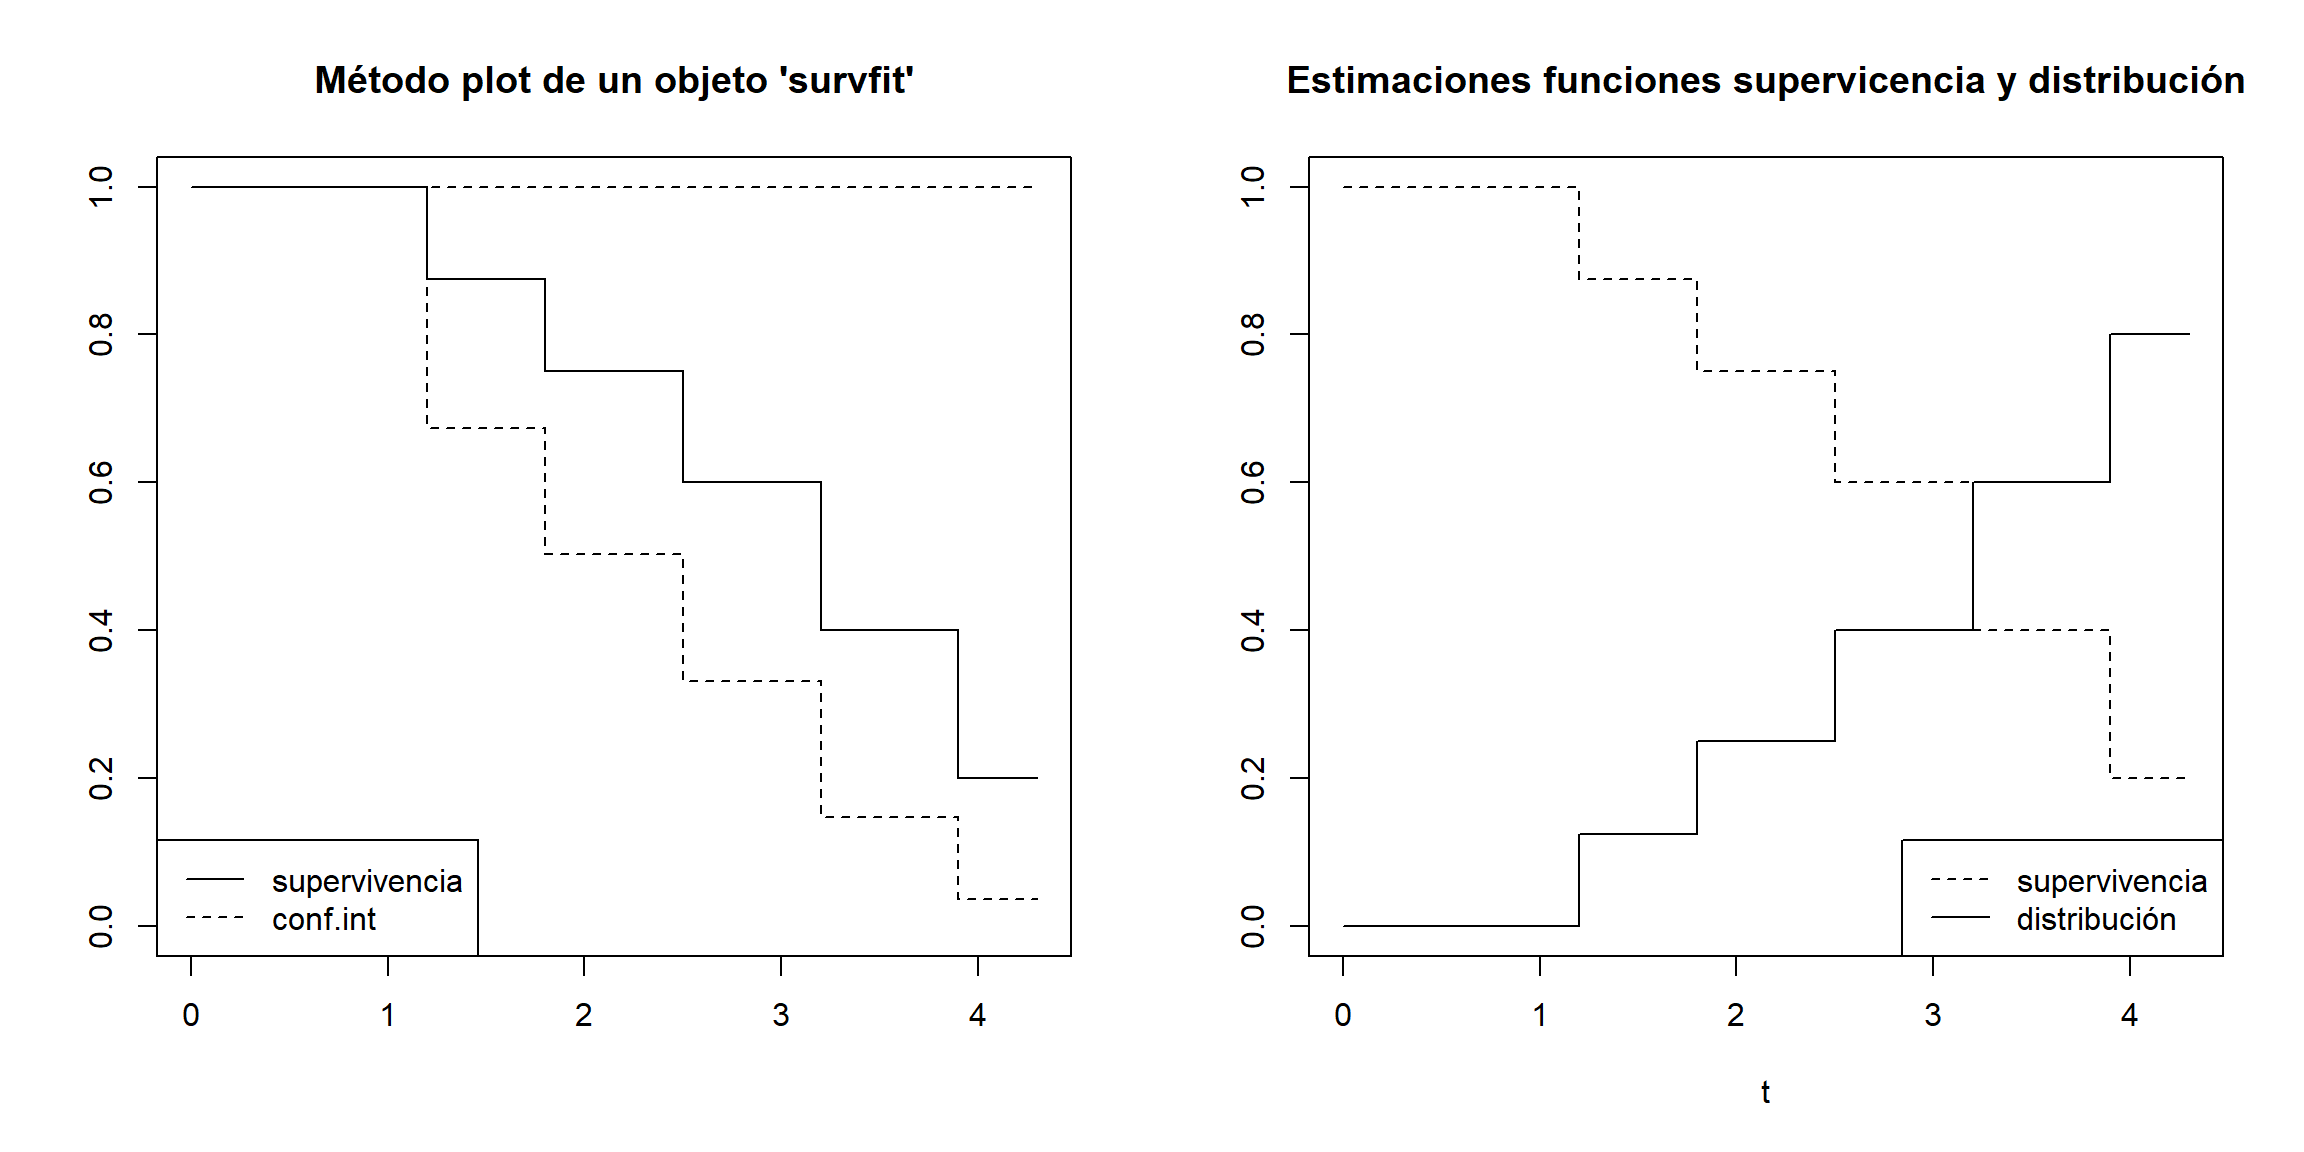
\includegraphics[width=0.7\linewidth]{08-dat_cen_files/figure-latex/survival-1} 

}

\caption{Estimaciones Kaplan-Meier de la función de supervivencia y de la función de distribución.}\label{fig:survival}
\end{figure}

\begin{Shaded}
\begin{Highlighting}[]
\KeywordTok{par}\NormalTok{(old.par)}
\end{Highlighting}
\end{Shaded}

\subsection{Distribución asintótica del estimador de
Kaplan-Meier}\label{distribucion-asintotica-del-estimador-de-kaplan-meier}

El estimador de Kaplan-Meier sólo otorga pesos positivos a los datos no
censurados, aunque la forma de distribuirse los datos censurados en
medio de los no censurados afecta a los pesos de estos últimos. Por otra
parte, en ausencia de censura (es decir \(\delta _i=1\),
\(i=1,2,\ldots ,n\)), el estimador de Kaplan-Meier coincide con la
distribución empírica.

La obtención de la propiedades de sesgo y varianza asintóticos y
distribución límite del estimador de Kaplan-Meier es mucho más laboriosa
que en el caso de la distribución empírica, en un contexto sin censura.
Esto es así porque el estimador de Kaplan-Meier deja de ser una suma de
variables iid, como sí ocurre con la empírica.

Breslow y Crowley (1974) obtienen el siguiente resultado para la
distribución límite para el estimador de Kaplan-Meier:
\[\sqrt{n}\left( \hat{F}\left( t \right) -F\left( t \right) \right) 
\overset{d}{\longrightarrow} \mathcal{N}\left( 0,\sigma^2\left( t \right)
\right),\] siendo \[\begin{aligned}
\sigma^2\left( t \right) &= \left( 1-F\left( t \right) \right)
^2\int_{0}^{t}\frac{dH_1\left( u \right)}{\left( 1-H\left( u \right)
 \right)^2}\text{, }t\leq H^{-1}(1) , \\
H_1\left( u \right) &= P\left( X\leq u,X\leq C \right) =P\left( T\leq
u,\delta =1 \right).
\end{aligned}\] También existen resultados de convergencia en
distribución del proceso estocástico
\[\left\{ \sqrt{n}\left( \hat{F}\left( t \right) - F\left( t \right)
 \right) : t \in \left[ 0,H^{-1}(1) \right] \right\}\] a un proceso
gaussiano límite.

\section{Remuestreos Bootstrap en presencia de
censura}\label{remuestreos-bootstrap-en-presencia-de-censura}

Estos métodos tratan del mecanismo bootstrap para aproximar la
distribución de un estadístico,
\(R\left( \mathbf{T}, \boldsymbol{\delta} \right)\), siendo
\(\mathbf{T}=\left( T_1, T_2, \ldots,T_n \right)\) y
\(\boldsymbol{\delta}=\left( \delta _1,\delta_2, \ldots ,\delta _n \right)\).
Los dos siguientes métodos de remuestreo fueron propuestos por Efron
(1981).

\subsection{El bootstrap simple}\label{el-bootstrap-simple}

Procede de la siguiente forma:

\begin{enumerate}
\def\labelenumi{\arabic{enumi}.}
\item
  Construir la distribución empírica bidimensional, \(F_n^{T,\delta }\),
  de la muestra
  \(\left\{ \left( T_1,\delta _1 \right), \left( T_2,\delta _2 \right), \ldots, \left( T_n,\delta _n \right) \right\}\).
\item
  Arrojar remuestras
  \(\left\{ \left( T_1^{\ast},\delta _1^{\ast} \right), \left( T_2^{\ast},\delta _2^{\ast} \right), \ldots, \left( T_n^{\ast},\delta _n^{\ast} \right) \right\}\)
  a partir de dicha distribución empírica. Esto es tanto como decir
  que\[P^{\ast}\left( \left( T^{\ast},\delta^{\ast} \right) =\left( T_i,\delta
  _i \right) \right) =\frac{1}{n}\text{, para }i=1,2,\ldots ,n\text{.}\]
\item
  Evaluar el estadístico de interés en el vector que contiene la
  remuestra bootstrap:
  \(R^{\ast}=R\left( \mathbf{T}^{\ast}, \boldsymbol{\delta}^{\ast} \right)\),
  con
  \(\mathbf{T}^{\ast} =\left( T_1^{\ast},T_2^{\ast},\ldots ,T_n^{\ast} \right)\)
  y

  \(\boldsymbol{\delta}^{\ast}=\left( \delta _1^{\ast},\delta _2^{\ast},\ldots ,\delta _n^{\ast} \right)\).
\item
  Aproximar la distribución en el muestreo del estadístico
  \(R\left( \mathbf{T}, \boldsymbol{\delta} \right)\) por la
  distribución en el remuestreo de
  \(R\left( \mathbf{T}^{\ast},\boldsymbol{\delta}^{\ast} \right)\).
\end{enumerate}

Este método es de muy rápida implementación y ejecución.

\subsection{El bootstrap obvio}\label{cap8-obvio}

Para detallar el método es necesario definir el estimador de
Kaplan-Meier, \(\hat{G}\left( t \right)\), de la variable censurante, a
partir
de\[1-\hat{G}\left( t \right) =\prod_{T_{(i)}\leq t}\left( \frac{n-i
}{n-i+1} \right)^{1-\delta _{(i)}}.\] Observemos que este estimador es
totalmente semejante al de Kaplan-Meier de la variable de interés pero
simplemente reemplazando cada valor \(\delta _{(i)}\) por
\(1-\delta _{(i)}\).

El mecanismo de remuestreo procede como sigue:

\begin{enumerate}
\def\labelenumi{\arabic{enumi}.}
\item
  Construir los estimadores de Kaplan-Meier de las distribuciones de la
  variable de interés, \(\hat{F}\left( t \right)\), y de la variable
  censurante, \(\hat{G}\left( t \right)\).
\item
  Para cada índice \(i=1,2,\ldots ,n\), arrojar observaciones bootstrap
  independientes, \(X_i^{\ast}\) con distribución \(\hat{F}\ \)y
  \(C_i^{\ast}\) con distribución \(\hat{G}\).
\item
  Definir \(T_i^{\ast}=\min \left\{ X_i^{\ast},C_i^{\ast}\right\}\) y
  \(\delta_i^{\ast}=\mathbf{1}_{\left\{ X_i^{\ast}\leq C_i^{\ast}\right\}}\),
  para \(i = 1, 2, \ldots, n\), y considerar la remuestra bootstrap
  \(\left( \mathbf{T}^{\ast},\boldsymbol{\delta}^{\ast}\right)\), con
  \(\mathbf{T}^{\ast}=\left( T_1^{\ast},T_2^{\ast}, \ldots, T_n^{\ast} \right)\)
  y
  \(\boldsymbol{\delta}^{\ast} = \left( \delta_1^{\ast}, \delta_2^{\ast},\ldots ,\delta_n^{\ast} \right)\).
\item
  Aproximar la distribución en el muestreo del estadístico
  \(R\left( \mathbf{T},\boldsymbol{\delta} \right)\) por la distribución
  en el remuestreo de su análogo bootstrap,
  \(R\left( \mathbf{T}^{\ast},\boldsymbol{\delta}^{\ast} \right)\).
\end{enumerate}

Obviamente, este método de remuestreo imita fielmente el modelo de datos
censurados por la derecha. Su ejecución es considerablemente más lenta
que la del método simple, pues necesita de la construcción de los
estimadores de Kaplan-Meier, de la obtención de remuestras a partir de
ellos y de algunos cálculos adicionales.

\section{Relaciones entre los métodos de remuestreo bajo
censura}\label{relaciones-entre-los-metodos-de-remuestreo-bajo-censura}

\subsection{Equivalencia entre el bootstrap simple y el
obvio}\label{equivalencia-entre-el-bootstrap-simple-y-el-obvio}

Es fácil demostrar que el bootstrap simple y el obvio son planes de
remuestreo equivalentes (cuando se supone que en la muestra no existe
ninguna observación no censurada que esté empatada con otra censurada).
Esta equivalencia se establece en el sentido de que la distribución
bootstrap de \(\left( T^{\ast},\delta^{\ast} \right)\) es la misma para
cualquiera de los dos métodos.

Así, si \(\left( T^{\ast},\delta^{\ast} \right)\) se genera mediante el
método obvio, entonces

\[\begin{aligned}
P^{\ast}\left( T^{\ast}>t \right) &= P^{\ast}\left( X^{\ast}>t,C^{\ast
}>t \right) \\
&= P^{\ast}\left( X^{\ast}>t \right) P^{\ast}\left( C^{\ast}>t \right)
=\left( 1-\hat{F}\left( t \right) \right) \left( 1-\hat{G}\left( t \right)
 \right) \\
&= \left[ \prod_{T_{(i)}\leq t}\left( \frac{n-i}{n-i+1} \right)
^{\delta _{(i)}}\right] \left[ \prod_{T_{(i)}\leq
t}\left( \frac{n-i}{n-i+1} \right)^{1-\delta _{(i)}}\right] \\
&= \prod_{T_{(i)}\leq t}\frac{n-i}{n-i+1}=\prod_{i=1}^{\#\left
\{ T_{(j)}\leq t\right\} }\frac{n-i}{n-i+1} \\
&= \frac{n-1}{n}\cdot \frac{n-2}{n-1}\cdot \cdots \cdot \frac{n-\#\left\{
T_{(j)}\leq t\right\} }{n-\#\left\{ T_{(j)}\leq
t\right\} +1} \\
&= \frac{n-\#\left\{ T_{(j)}\leq t\right\} }{n}=1-H_n\left(
t \right) =\frac{\#\left\{ T_{(j)}>t\right\} }{n},
\end{aligned}\]

siendo \(H_n\left( t \right)\) la distribución empírica de la muestra
\(\left( T_1,T_2,\ldots ,T_n \right)\).

Esto demuestra que la distribución bootstrap marginal de \(T^{\ast}\) es
la misma para ambos remuestreos. Sólo resta probar pues que la
distribución condicionada
\(\left. \delta^{\ast}\right\vert _{T^{\ast}=T_i}\) es idéntica en ambos
casos. Pero esto es inmediato ya que, en los dos remuestreos esa
distribución condicionada es la degenerada en el valor \(\delta _i\).

\subsection{El bootstrap de Reid}\label{cap8-reid}

Es otro método alternativo propuesto por Reid (1981). Consta de los
siguientes pasos:

\begin{enumerate}
\def\labelenumi{\arabic{enumi}.}
\item
  Construir el estimador de Kaplan-Meier, \(\hat{F}\left( t \right)\),
  de la muestra original.
\item
  Arrojar remuestras bootstrap (todas formadas por observaciones no
  censuradas, \(T_i^{\ast}\), \(i=1,2,\ldots ,n\)) a partir de
  \(\hat{F}\left(t \right)\).
\item
  Aproximar la distribución en el muestreo de
  \(R\left( \mathbf{T},\boldsymbol{\delta} \right)\), por la
  distribución bootstrap de
  \(R\left( \mathbf{T}^{\ast},\mathbf{1} \right)\), siendo
  \(\mathbf{1}\) el vector formado por \(n\) unos.
\end{enumerate}

\subsection{Validez de los planes de
remuestreo}\label{validez-de-los-planes-de-remuestreo}

Akritas (1986) demuestra que los procesos bootstrap \[\begin{aligned}
\sqrt{n}\left( \hat{F}^{\ast}_{Efron}\left( t \right) 
- \hat{F}\left( t \right) \right) \\ 
\sqrt{n}\left( \hat{F}^{\ast}_{Reid} \left( t \right) 
- \hat{F}\left( t \right) \right)
\end{aligned}\] tienden a sendos procesos límite distintos. Aquí
\(\hat{F}^{\ast}_{Efron}\) denota la versión bootstrap del estimador de
Kaplan-Meier bajo el remuestreo de Efron (cualquiera de ellos, ya que el
remuestreo simple y el obvio son equivalentes) y
\(\hat{F}^{\ast}_{Reid}\) es la correspondiente versión bootstrap del
estimador de Kaplan-Meier bajo el remuestreo de Reid (una distribución
empírica, al fin y al cabo, porque en el remuestreo de Reid todas las
observaciones son no censuradas).

Además el proceso límite del estimador de Kaplan-Meier,
\(\sqrt{n} \left( \hat{F}\left( t \right) -F\left( t \right) \right)\),
es el mismo que el del bootstrap de Efron. Como consecuencia el
remuestreo de Efron es consistente y el de Reid es inconsistente.

\section{\texorpdfstring{Implementación en \texttt{R} (con los paquetes
\texttt{boot} y
\texttt{survival})}{Implementación en R (con los paquetes boot y survival)}}\label{implementacion-en-r-con-los-paquetes-boot-y-survival}

La función \texttt{censboot()} del paquete \texttt{boot} implementa
distintos métodos de remuestreo para datos censurados. Por defecto
utiliza el bootstrap simple (\texttt{sim\ =\ "ordinary"}) y su uso es
prácticamente igual al del bootstrap uniforme con la función
\texttt{boot()} (descrita en la Sección \ref{cap1-pkgboot}), la única
diferencia es que la función \texttt{statistic} solo tiene los datos
como único parámetro (aunque en este caso podríamos emplear también la
función \texttt{boot()}).

\subsection{Bootstrap simple}\label{bootstrap-simple}

Como ejemplo utilizaremos el conjunto de datos \texttt{channing} del
paquete \texttt{boot}, que contiene la edad de entrada y de partida o
muerte de las personas que pasaron por el centro de retiro `Channing
House' (Palo Alto, California), desde su apertura en 1964 hasta el 1 de
julio de 1975 (ver Sección 3.5 y `Practical 3.2', de Davison y Hinkley,
1997). En primer lugar consideraremos únicamente la muestra de hombres:

\begin{Shaded}
\begin{Highlighting}[]
\CommentTok{# Datos}
\KeywordTok{library}\NormalTok{(boot)}
\KeywordTok{data}\NormalTok{(channing)}
\CommentTok{# Calcular edad (de partida o muerte) en años}
\NormalTok{channing}\OperatorTok{$}\NormalTok{age <-}\StringTok{ }\NormalTok{(channing}\OperatorTok{$}\NormalTok{entry }\OperatorTok{+}\StringTok{ }\NormalTok{channing}\OperatorTok{$}\NormalTok{time)}\OperatorTok{/}\DecValTok{12}
\CommentTok{# Seleccionar hombres (y de paso hacer que `index = c(1, 2)` para `censboot()`)}
\NormalTok{chan <-}\StringTok{ }\KeywordTok{subset}\NormalTok{(channing, sex}\OperatorTok{==}\StringTok{"Male"}\NormalTok{, }\KeywordTok{c}\NormalTok{(age, cens))}

\CommentTok{# Estimación supervivencia}
\KeywordTok{library}\NormalTok{(survival)}
\NormalTok{chan.F <-}\StringTok{ }\KeywordTok{survfit}\NormalTok{(}\KeywordTok{Surv}\NormalTok{(age, cens)}\OperatorTok{~}\DecValTok{1}\NormalTok{, }\DataTypeTok{data =}\NormalTok{ chan)}
\NormalTok{chan.F}
\end{Highlighting}
\end{Shaded}

\begin{verbatim}
## Call: survfit(formula = Surv(age, cens) ~ 1, data = chan)
## 
##       n  events  median 0.95LCL 0.95UCL 
##    97.0    46.0    87.0    85.8    90.4
\end{verbatim}

\begin{Shaded}
\begin{Highlighting}[]
\CommentTok{# plot(chan.F)}
\CommentTok{# Estimaciones de interés}
\KeywordTok{with}\NormalTok{(chan.F, }
    \KeywordTok{c}\NormalTok{(}\DataTypeTok{s75 =} \KeywordTok{max}\NormalTok{(surv[time }\OperatorTok{>}\StringTok{ }\DecValTok{75}\NormalTok{]), }\DataTypeTok{s85 =} \KeywordTok{max}\NormalTok{(surv[time }\OperatorTok{>}\StringTok{ }\DecValTok{85}\NormalTok{]),}
      \DataTypeTok{p75 =} \KeywordTok{min}\NormalTok{(time[surv }\OperatorTok{<=}\StringTok{ }\FloatTok{0.75}\NormalTok{]), }\DataTypeTok{p50 =} \KeywordTok{min}\NormalTok{(time[surv }\OperatorTok{<=}\StringTok{ }\FloatTok{0.5}\NormalTok{])) }
\NormalTok{)}
\end{Highlighting}
\end{Shaded}

\begin{verbatim}
##        s75        s85        p75        p50 
##  0.9160745  0.6347541 82.4166667 87.0000000
\end{verbatim}

\begin{Shaded}
\begin{Highlighting}[]
\CommentTok{# Bootstrap}
\CommentTok{# library(boot)}
\NormalTok{chan.stat <-}\StringTok{ }\ControlFlowTok{function}\NormalTok{(data) \{}
\NormalTok{    s <-}\StringTok{ }\KeywordTok{survfit}\NormalTok{(}\KeywordTok{Surv}\NormalTok{(age, cens)}\OperatorTok{~}\DecValTok{1}\NormalTok{, }\DataTypeTok{data =}\NormalTok{ data)}
    \KeywordTok{with}\NormalTok{(s, }\KeywordTok{c}\NormalTok{(}\DataTypeTok{s75 =} \KeywordTok{max}\NormalTok{(surv[time }\OperatorTok{>}\StringTok{ }\DecValTok{75}\NormalTok{]), }\DataTypeTok{s85 =} \KeywordTok{max}\NormalTok{(surv[time }\OperatorTok{>}\StringTok{ }\DecValTok{85}\NormalTok{]),}
            \DataTypeTok{p75 =} \KeywordTok{min}\NormalTok{(time[surv }\OperatorTok{<=}\StringTok{ }\FloatTok{0.75}\NormalTok{]), }\DataTypeTok{p50 =} \KeywordTok{min}\NormalTok{(time[surv }\OperatorTok{<=}\StringTok{ }\FloatTok{0.5}\NormalTok{])))}
\NormalTok{\}}
\KeywordTok{set.seed}\NormalTok{(}\DecValTok{1}\NormalTok{)}
\NormalTok{chan.boot <-}\StringTok{ }\KeywordTok{censboot}\NormalTok{(chan, chan.stat, }\DataTypeTok{R =} \DecValTok{199}\NormalTok{) }\CommentTok{# sim = "ordinary"}
\NormalTok{chan.boot}
\end{Highlighting}
\end{Shaded}

\begin{verbatim}
## 
## CASE RESAMPLING BOOTSTRAP FOR CENSORED DATA
## 
## 
## Call:
## censboot(data = chan, statistic = chan.stat, R = 199)
## 
## 
## Bootstrap Statistics :
##       original       bias    std. error
## t1*  0.9160745 -0.010197967  0.03107258
## t2*  0.6347541 -0.006979654  0.05572596
## t3* 82.4166667 -0.061139028  1.23839853
## t4* 87.0000000  0.195142379  1.09877565
\end{verbatim}

\subsection{Otros métodos de
remuestreo}\label{otros-metodos-de-remuestreo}

La función \texttt{censboot()} implementa otros dos métodos de
remuestreo, \texttt{sim\ =\ c("cond",\ "weird")}, aunque en ambos casos
hay que establecer en el parámetro \texttt{F.surv} la estimación de
Kaplan-Meier de la supervivencia y, si \texttt{sim\ =\ "cond"}, la
correspondiente a la variable censurante en \texttt{G.surv}. Se
recomienda estimarlas con la función \texttt{survfit()} del paquete
\texttt{survival} (ver Figura \ref{fig:survfit-f-g}):

\begin{Shaded}
\begin{Highlighting}[]
\CommentTok{# Estimación supervivencia variable censurante}
\NormalTok{chan.G <-}\StringTok{ }\KeywordTok{survfit}\NormalTok{(}\KeywordTok{Surv}\NormalTok{(age, }\DecValTok{1}\OperatorTok{-}\NormalTok{cens)}\OperatorTok{~}\DecValTok{1}\NormalTok{, }\DataTypeTok{data =}\NormalTok{ chan)}
\CommentTok{# Representación}
\NormalTok{old.par <-}\StringTok{ }\KeywordTok{par}\NormalTok{(}\DataTypeTok{mfrow =} \KeywordTok{c}\NormalTok{(}\DecValTok{1}\NormalTok{, }\DecValTok{2}\NormalTok{))}
\KeywordTok{plot}\NormalTok{(chan.F, }\DataTypeTok{main =} \StringTok{"Supervivencia (edad)"}\NormalTok{, }\DataTypeTok{mark.time =} \OtherTok{TRUE}\NormalTok{, }
    \DataTypeTok{xlim =} \KeywordTok{c}\NormalTok{(}\DecValTok{60}\NormalTok{, }\DecValTok{100}\NormalTok{))}
\KeywordTok{plot}\NormalTok{(chan.G, }\DataTypeTok{main =} \StringTok{"Supervivencia variable censurante (partida)"}\NormalTok{, }
     \DataTypeTok{mark.time =} \OtherTok{TRUE}\NormalTok{, }\DataTypeTok{xlim =} \KeywordTok{c}\NormalTok{(}\DecValTok{60}\NormalTok{, }\DecValTok{100}\NormalTok{))}
\end{Highlighting}
\end{Shaded}

\begin{figure}[!htb]

{\centering 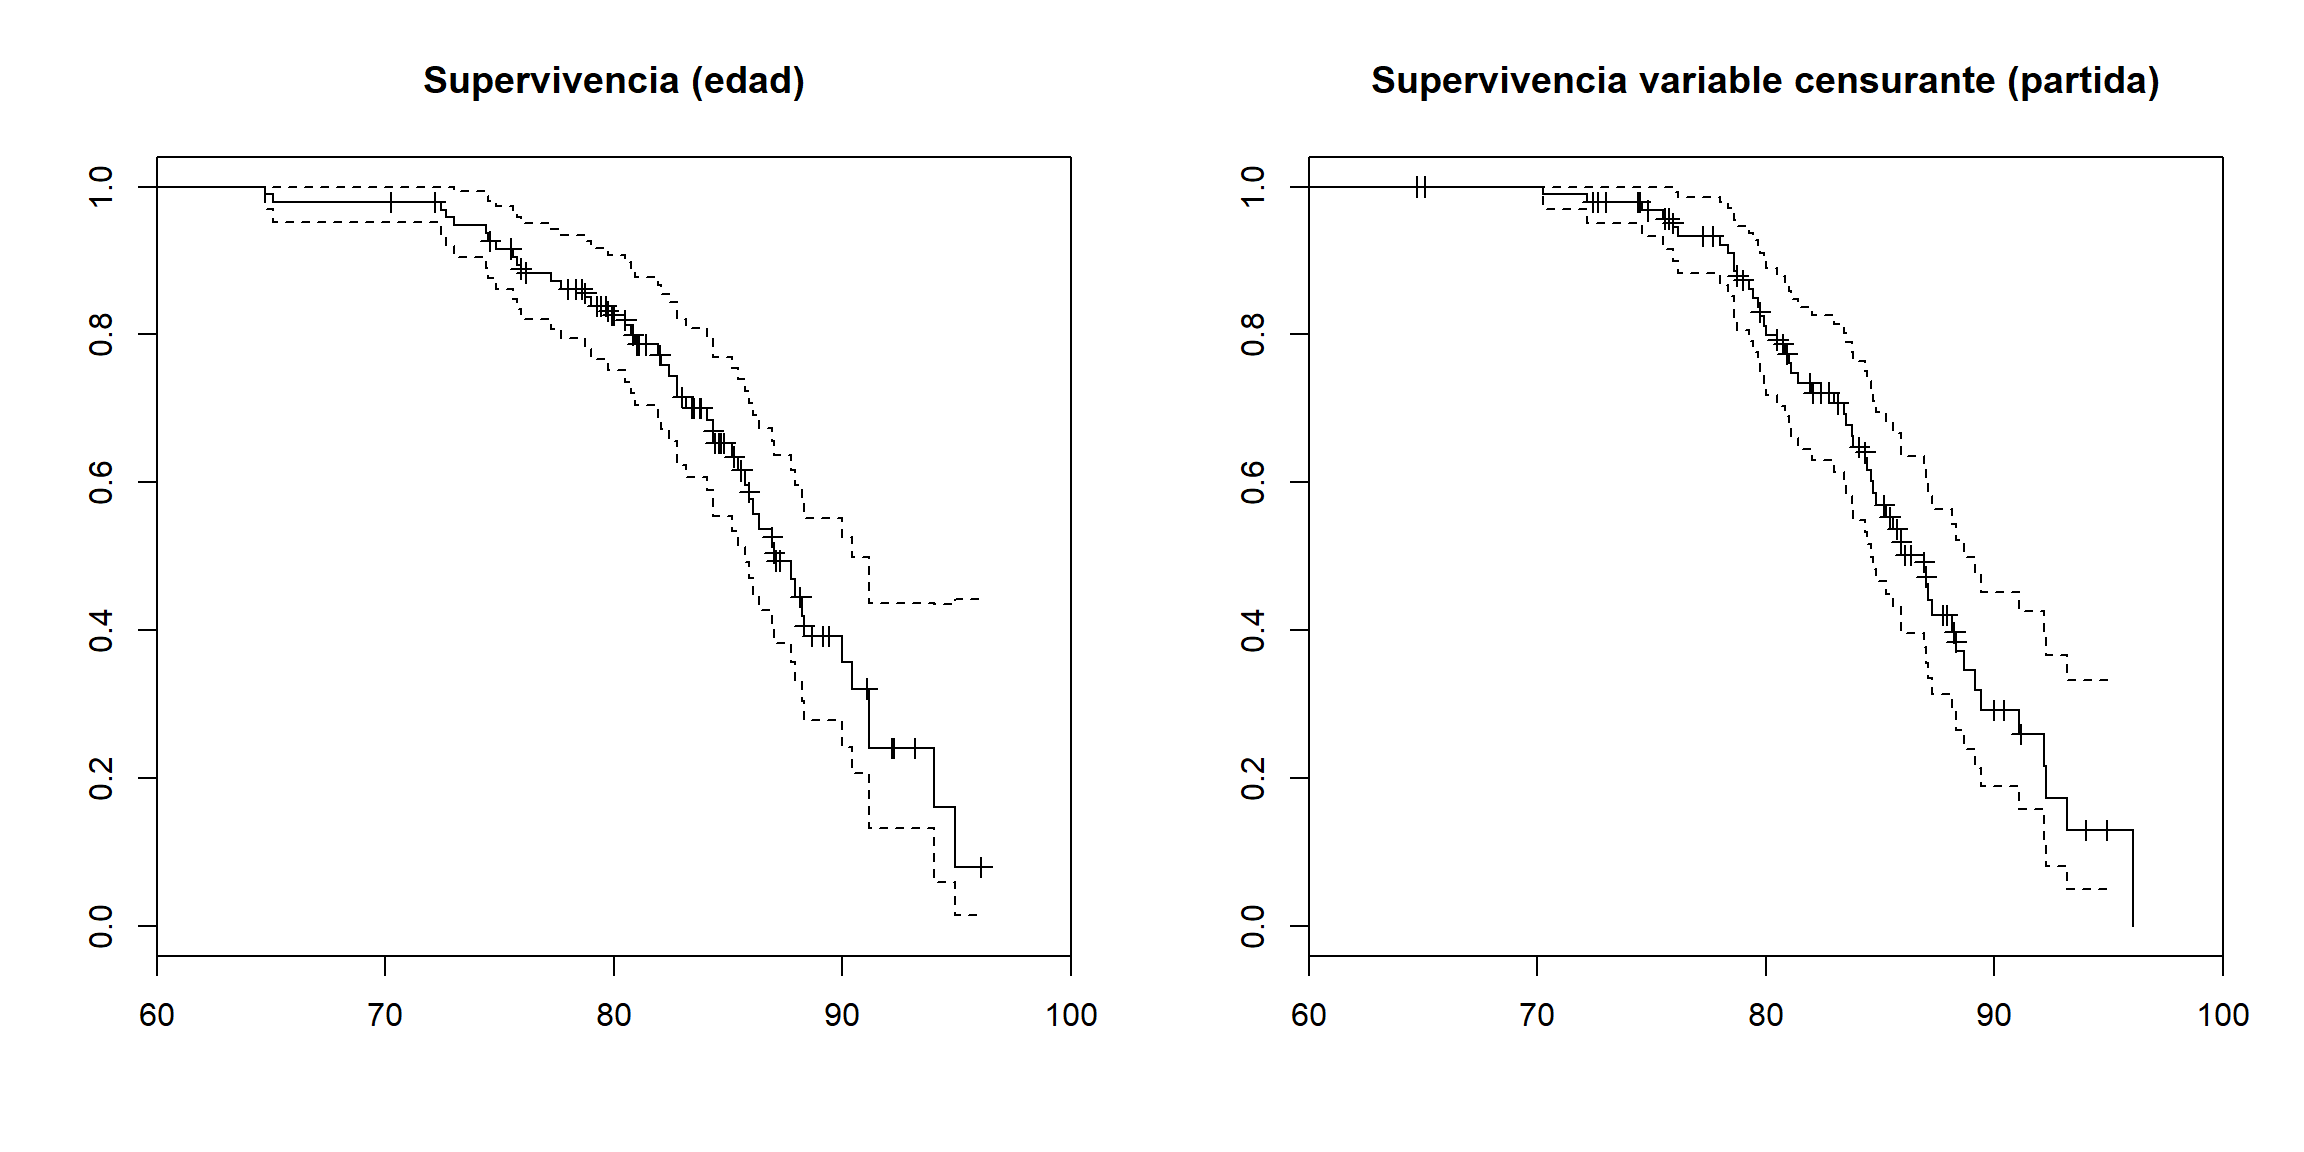
\includegraphics[width=0.7\linewidth]{08-dat_cen_files/figure-latex/survfit-f-g-1} 

}

\caption{Estimaciones de la supervivencia (izquierda; indicando los tiempos de las observaciones censuradas) y de la variable censurante (derecha; indicando los de las no censuradas).}\label{fig:survfit-f-g}
\end{figure}

\begin{Shaded}
\begin{Highlighting}[]
\KeywordTok{par}\NormalTok{(old.par)}
\end{Highlighting}
\end{Shaded}

En el \emph{boostrap condicional} (\texttt{sim\ =\ "cond"}) se
condiciona el muestreo al patrón de censura observado (en lugar de
fijarlo a \(\mathbf{1}\) como en el bootstrap de Reid; Sección
\ref{cap8-reid}). El mecanismo es similar al del bootstrap obvio
(Sección \ref{cap8-obvio}):

\begin{enumerate}
\def\labelenumi{\arabic{enumi}.}
\item
  Construir los estimadores de Kaplan-Meier de las distribuciones de la
  variable de interés, \(\hat{F}\left( t \right)\), y de la variable
  censurante, \(\hat{G}\left( t \right)\).
\item
  Para cada índice \(i=1,2,\ldots ,n\), generar \(X_i^{\ast}\)
  independientes con distribución \(\hat{F}\).
\item
  Si la \(i\)-ésima observación está censurada (\(\delta_i=0\)) se toma
  \(C_i^{\ast}=X_i\) y si no (\(\delta_i=1\)) se genera un valor de la
  estimación de la distribución de la variable censurante condicionada a
  \(C > X_i\):
  \[\hat G \left(\left. t \ \right\vert_{\ t > X_i} \right) 
  = \frac{\hat G(t) - \hat G(X_i)}{1- \hat G(X_i)}.\]
\item
  Definir \(T_i^{\ast}=\min \left\{ X_i^{\ast},C_i^{\ast}\right\}\) y
  \(\delta_i^{\ast}=\mathbf{1}_{\left\{ X_i^{\ast}\leq C_i^{\ast}\right\}}\),
  para \(i = 1, 2, \ldots, n\), y considerar la remuestra bootstrap
  \(\left( \mathbf{T}^{\ast},\boldsymbol{\delta}^{\ast}\right)\), con
  \(\mathbf{T}^{\ast}=\left( T_1^{\ast},T_2^{\ast}, \ldots, T_n^{\ast} \right)\)
  y
  \(\boldsymbol{\delta}^{\ast} = \left( \delta_1^{\ast}, \delta_2^{\ast},\ldots ,\delta_n^{\ast} \right)\).
\end{enumerate}

El otro método (\texttt{sim\ =\ "weird"}) es el denominado \emph{weird
bootstrap} (Andersen et al., 1993) que emplea la estimación de
Nelson-Aalen de la función de riesgo acumulada para generar los valores
(e.g.~Sección 3.5.2 de Davison y Hinkley, 1997).

El siguiente código muestra un ejemplo de la aplicación de ambos
métodos:

\begin{Shaded}
\begin{Highlighting}[]
\NormalTok{chan.boot2 <-}\StringTok{ }\KeywordTok{censboot}\NormalTok{(chan, chan.stat, }\DataTypeTok{R =} \DecValTok{199}\NormalTok{, }\DataTypeTok{F.surv =}\NormalTok{ chan.F, }
                  \DataTypeTok{G.surv =}\NormalTok{ chan.G, }\DataTypeTok{sim =} \StringTok{"cond"}\NormalTok{)}
\NormalTok{chan.boot2}
\end{Highlighting}
\end{Shaded}

\begin{verbatim}
## 
## CONDITIONAL BOOTSTRAP FOR CENSORED DATA
## 
## 
## Call:
## censboot(data = chan, statistic = chan.stat, R = 199, F.surv = chan.F, 
##     G.surv = chan.G, sim = "cond")
## 
## 
## Bootstrap Statistics :
##       original       bias    std. error
## t1*  0.9160745  0.001487588  0.02733430
## t2*  0.6347541 -0.002352270  0.05369653
## t3* 82.4166667  0.056113903  1.09585116
## t4* 87.0000000  0.311557789  1.07687814
\end{verbatim}

\begin{Shaded}
\begin{Highlighting}[]
\NormalTok{chan.boot3 <-}\StringTok{ }\KeywordTok{censboot}\NormalTok{(chan, chan.stat, }\DataTypeTok{R =} \DecValTok{199}\NormalTok{, }\DataTypeTok{F.surv =}\NormalTok{ chan.F, }
                  \DataTypeTok{sim =} \StringTok{"weird"}\NormalTok{)}
\NormalTok{chan.boot3}
\end{Highlighting}
\end{Shaded}

\begin{verbatim}
## 
## WEIRD BOOTSTRAP FOR CENSORED DATA
## 
## 
## Call:
## censboot(data = chan, statistic = chan.stat, R = 199, F.surv = chan.F, 
##     sim = "weird")
## 
## 
## Bootstrap Statistics :
##       original        bias    std. error
## t1*  0.9160745 -0.0009515623  0.02451369
## t2*  0.6347541 -0.0046012462  0.04549111
## t3* 82.4166667 -0.0477386935  1.05510180
## t4* 87.0000000  0.2985762144  0.94422869
\end{verbatim}

\section{Ejercicios}\label{ejercicios}

\BeginKnitrBlock{exercise}[Bootstrap censurado por estratos]
\protect\hypertarget{exr:censboot-strata-ej}{}{\label{exr:censboot-strata-ej}
\iffalse (Bootstrap censurado por estratos) \fi{} } Analizar el conjunto
de datos \texttt{channing} completo, teniendo en cuenta el sexo como
estrato (i.e. \texttt{Surv(age,\ cens)\ \textasciitilde{}\ sex} y
\texttt{strata\ =\ chan\$sex})
\EndKnitrBlock{exercise}

\begin{Shaded}
\begin{Highlighting}[]
\CommentTok{# Datos}
\KeywordTok{data}\NormalTok{(channing)}
\CommentTok{# Calcular edad (de partida o muerte) en años}
\NormalTok{channing}\OperatorTok{$}\NormalTok{age <-}\StringTok{ }\NormalTok{(channing}\OperatorTok{$}\NormalTok{entry }\OperatorTok{+}\StringTok{ }\NormalTok{channing}\OperatorTok{$}\NormalTok{time)}\OperatorTok{/}\DecValTok{12}
\CommentTok{# Seleccionar variables}
\NormalTok{chan <-channing[}\KeywordTok{c}\NormalTok{(}\StringTok{"age"}\NormalTok{, }\StringTok{"cens"}\NormalTok{, }\StringTok{"sex"}\NormalTok{)]}

\CommentTok{# Estimación supervivencia}
\KeywordTok{library}\NormalTok{(survival)}
\NormalTok{chan.F <-}\StringTok{ }\KeywordTok{survfit}\NormalTok{(}\KeywordTok{Surv}\NormalTok{(age, cens) }\OperatorTok{~}\StringTok{ }\NormalTok{sex, }\DataTypeTok{data =}\NormalTok{ chan)}
\NormalTok{chan.F}
\end{Highlighting}
\end{Shaded}

\begin{verbatim}
## Call: survfit(formula = Surv(age, cens) ~ sex, data = chan)
## 
##              n events median 0.95LCL 0.95UCL
## sex=Female 365    130     88    86.7    89.5
## sex=Male    97     46     87    85.8    90.4
\end{verbatim}

\begin{Shaded}
\begin{Highlighting}[]
\KeywordTok{plot}\NormalTok{(chan.F, }\DataTypeTok{lty =} \DecValTok{1}\OperatorTok{:}\DecValTok{2}\NormalTok{, }\DataTypeTok{xlim =} \KeywordTok{c}\NormalTok{(}\DecValTok{60}\NormalTok{, }\DecValTok{100}\NormalTok{))}
\end{Highlighting}
\end{Shaded}

\begin{figure}[!htb]

{\centering 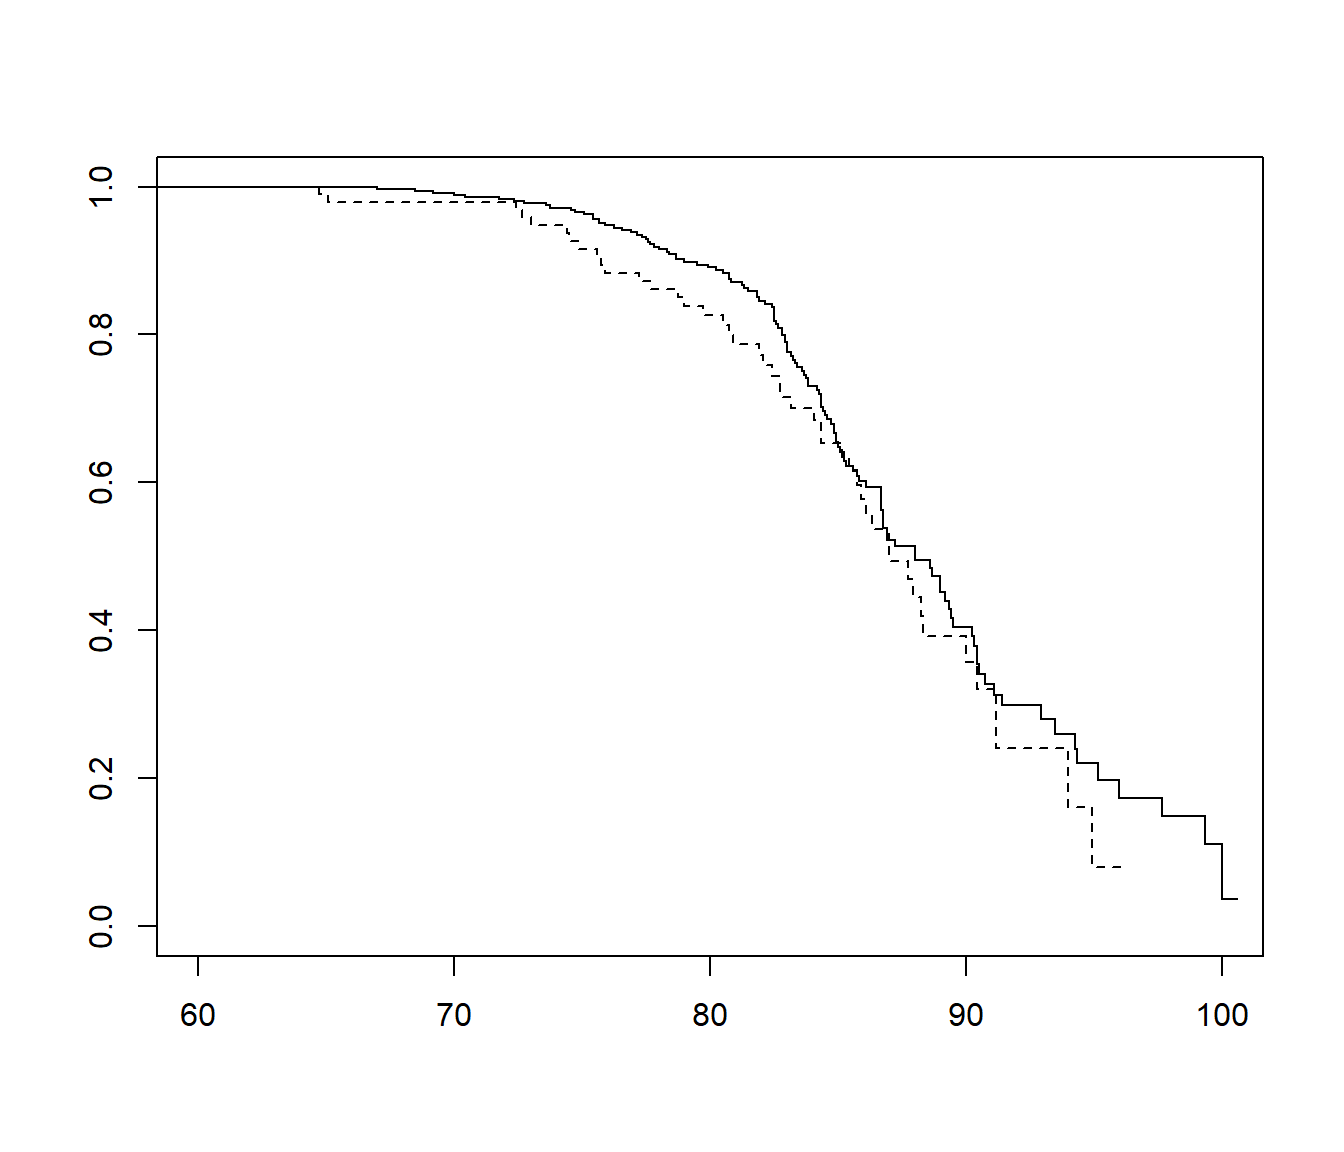
\includegraphics[width=0.7\linewidth]{08-dat_cen_files/figure-latex/surv-strata-1} 

}

\caption{Estimaciones de la supervivencia.}\label{fig:surv-strata}
\end{figure}

\begin{Shaded}
\begin{Highlighting}[]
\NormalTok{res <-}\StringTok{ }\KeywordTok{summary}\NormalTok{(chan.F)}
\CommentTok{# res}
\KeywordTok{str}\NormalTok{(res)}
\end{Highlighting}
\end{Shaded}

\begin{verbatim}
## List of 16
##  $ n            : int [1:2] 365 97
##  $ time         : num [1:146] 67 68.5 69.2 70 70.4 ...
##  $ n.risk       : num [1:146] 364 359 355 353 352 346 344 340 335 334 ...
##  $ n.event      : num [1:146] 1 1 1 1 1 1 1 1 1 1 ...
##  $ n.censor     : num [1:146] 2 3 3 1 0 6 0 3 4 0 ...
##  $ surv         : num [1:146] 0.997 0.994 0.992 0.989 0.986 ...
##  $ type         : chr "right"
##  $ strata       : Factor w/ 2 levels "sex=Female","sex=Male": 1 1 1 1 1 1 1 1 1 1 ...
##  $ std.err      : num [1:146] 0.00274 0.0039 0.00479 0.00554 0.00619 ...
##  $ lower        : num [1:146] 0.992 0.987 0.982 0.978 0.974 ...
##  $ upper        : num [1:146] 1 1 1 1 0.998 ...
##  $ conf.type    : chr "log"
##  $ conf.int     : num 0.95
##  $ call         : language survfit(formula = Surv(age, cens) ~ sex, data = chan)
##  $ table        : num [1:2, 1:9] 365 97 365 97 365 ...
##   ..- attr(*, "dimnames")=List of 2
##   .. ..$ : chr [1:2] "sex=Female" "sex=Male"
##   .. ..$ : chr [1:9] "records" "n.max" "n.start" "events" ...
##  $ rmean.endtime: num [1:2] 98.3 98.3
##  - attr(*, "class")= chr "summary.survfit"
\end{verbatim}

\begin{Shaded}
\begin{Highlighting}[]
\CommentTok{# Estimaciones de interés}
\NormalTok{res}\OperatorTok{$}\NormalTok{table[, }\KeywordTok{c}\NormalTok{(}\StringTok{"*rmean"}\NormalTok{, }\StringTok{"median"}\NormalTok{)]}
\end{Highlighting}
\end{Shaded}

\begin{verbatim}
##              *rmean median
## sex=Female 88.21716     88
## sex=Male   86.71872     87
\end{verbatim}

\begin{Shaded}
\begin{Highlighting}[]
\KeywordTok{as.numeric}\NormalTok{(res}\OperatorTok{$}\NormalTok{table[, }\KeywordTok{c}\NormalTok{(}\StringTok{"*rmean"}\NormalTok{, }\StringTok{"median"}\NormalTok{)])}
\end{Highlighting}
\end{Shaded}

\begin{verbatim}
## [1] 88.21716 86.71872 88.00000 87.00000
\end{verbatim}

\BeginKnitrBlock{exercise}[Bootstrap censurado con riesgo proporcional de Cox]
\protect\hypertarget{exr:censboot-cox-ej}{}{\label{exr:censboot-cox-ej}
\iffalse (Bootstrap censurado con riesgo proporcional de Cox) \fi{} }
Reproducir el ejemplo en Canty (2002,
\href{http://cran.fhcrc.org/doc/Rnews/Rnews_2002-3.pdf}{Rnews\_2002-3})
del modelo de riesgo proporcional de Cox (Cox, 1972):
\EndKnitrBlock{exercise}

\begin{Shaded}
\begin{Highlighting}[]
\CommentTok{# Datos}
\KeywordTok{data}\NormalTok{(melanoma)}
\NormalTok{mel <-}\StringTok{ }\NormalTok{melanoma[melanoma}\OperatorTok{$}\NormalTok{ulcer }\OperatorTok{==}\StringTok{ }\DecValTok{1}\NormalTok{, ]}
\NormalTok{mel}\OperatorTok{$}\NormalTok{cens <-}\StringTok{ }\DecValTok{1} \OperatorTok{*}\StringTok{ }\NormalTok{(mel}\OperatorTok{$}\NormalTok{status }\OperatorTok{==}\StringTok{ }\DecValTok{1}\NormalTok{)}
\CommentTok{# Estimación supervivencia}
\KeywordTok{library}\NormalTok{(survival)}
\CommentTok{# Modelo de riesgo proporcional de Cox}
\NormalTok{mel.cox <-}\StringTok{ }\KeywordTok{coxph}\NormalTok{(}\KeywordTok{Surv}\NormalTok{(time, cens) }\OperatorTok{~}\StringTok{ }\NormalTok{thickness, }\DataTypeTok{data =}\NormalTok{ mel)}
\NormalTok{mel.cox}
\end{Highlighting}
\end{Shaded}

\begin{verbatim}
## Call:
## coxph(formula = Surv(time, cens) ~ thickness, data = mel)
## 
##             coef exp(coef) se(coef)    z     p
## thickness 0.0997    1.1048   0.0405 2.46 0.014
## 
## Likelihood ratio test=5  on 1 df, p=0.03
## n= 90, number of events= 41
\end{verbatim}

\begin{Shaded}
\begin{Highlighting}[]
\CommentTok{# summary(mel.cox)}
\CommentTok{# Estadísticos de interés}
\NormalTok{mel.cox}\OperatorTok{$}\NormalTok{coefficients}
\end{Highlighting}
\end{Shaded}

\begin{verbatim}
##  thickness 
## 0.09967665
\end{verbatim}

\chapter{El Bootstrap con datos dependientes}\label{cap9}

En este capítulo se presentan gran cantidad de métodos bootstrap para
realizar inferencia, así como predicción, en el contexto de datos
dependientes. En primer lugar se hace una introducción a las condiciones
habituales de dependencia y a los modelo paramétricos de dependencia,
para luego centrarse en los métodos de remuestreo en ambos contextos.

En cada uno de los dos contextos (estimación y predicción) se estudiarán
dos situaciones drásticamente diferentes. En la primera de ellas
consideraremos modelos en los que la estructura de dependencia está
explícitamente modelizada (normalmente a través de una ecuación de
autorregresión), mientras que la segunda trata el caso en que no existe
ninguna especificación explícita de la estructura de dependencia
(simplemente se asumen condiciones mixing, por ejemplo). Una revisión
sobre los resultados principales puede verse en Cao (1999).

\section{Introducción a las condiciones de dependencia y modelos
habituales de datos
dependientes}\label{introduccion-a-las-condiciones-de-dependencia-y-modelos-habituales-de-datos-dependientes}

\subsection{Situaciones de dependencia
general}\label{situaciones-de-dependencia-general}

Consideramos un proceso estocástico en tiempo discreto y con espacio de
estados continuo (p.~ej. \(\mathbb{R}\)),
\(\left\{X_{t}\right\}_{t\in \mathbb{Z}}\), del cual observamos parte de
su trayectoria: \(\left( X_1,X_2,\ldots ,X_n \right)\), es decir una
muestra de datos dependientes. Este tipo de procesos estocásticos suelen
llamarse series temporales.

Normalmente supondremos que el proceso
\(\left\{ X_{t}\right\}_{t\in \mathbb{Z}}\) es estacionario. En
ocasiones se requerirá además que sea fuertemente mixing:
\[\sup_{A\in \mathcal{F}_1^{n},B\in \mathcal{F}_{n+k}^{\infty }}\left\vert
P\left( A\cap B \right) -P\left( A \right) P(B) \right\vert \leq
\alpha _{k}\text{, con }\alpha _{k}\rightarrow 0,\] o bien uniformemente
mixing:
\[\left\vert P\left( A\cap B \right) -P\left( A \right) P(B) \right\vert 
\leq \phi _{k}P\left( A \right) \text{, }\forall A\in \mathcal{F}_1^{n},
\forall B\in \mathcal{F}_{n+k}^{\infty }\text{, con }\phi_{k}\rightarrow 0,\]
siendo \(\mathcal{F}_{s}^{t}\) la \(\sigma\)-algebra generada por las
variables aleatorias \(X_{s},\ldots ,X_{t}\).

Estas condiciones establecen que la dependencia entre las variables
aleatorias que conforman las observaciones de la muestra se atenúa a
medida que sus instantes temporales se distancian.

\subsection{Modelos paramétricos de
dependencia}\label{modelos-parametricos-de-dependencia}

Los modelos paramétricos más habituales para datos dependientes y
estacionarios son los autorregresivos (\(AR\left( p \right)\)):
\[X_{t}=\phi _1X_{t-1}+\phi _2X_{t-2}+\cdots +\phi _{p}X_{t-p}+a_{t}
\text{, }t\in \mathbb{Z},\] de medias móviles (\(MA\left( q \right)\)):
\[X_{t}=a_{t}-\theta _1a_{t-1}-\theta _2a_{t-2}-\cdots -\theta _{p}a_{t-q}
\text{, }t\in \mathbb{Z}\] y la mezcla de ambos
(\(ARMA\left( p,q \right)\)): \[\begin{aligned}
X_{t} =&\ \phi _1X_{t-1}+\phi _2X_{t-2}+\cdots +\phi _{p}X_{t-p} \\
&+a_{t}-\theta _1a_{t-1}-\theta _2a_{t-2}-\cdots -\theta _{q}a_{t-q},\end{aligned}\]
En las anteriores expresiones los
\(\left\{ a_{t}\right\} _{t\in \mathbb{Z}}\) representan una sucesión de
variables independientes con la misma distribución (ruido blanco),
habitualmente con distribución normal.

\section{El bootstrap en la estimación con datos
dependientes}\label{el-bootstrap-en-la-estimacion-con-datos-dependientes}

El objetivo de esta sección es mostrar distintos métodos de remuestreo
para realizar inferencia sobre los parámetros de una serie temporal.
Comenzaremos tratando los modelos de dependencia explícita para luego
abordar la situación en que tan sólo existen condiciones generales de
dependencia.

\subsection{Modelos paramétricos de
dependencia}\label{modelos-parametricos-de-dependencia-1}

Consideremos uno de los casos más simples, dado por el modelo \(AR(p)\):
\[X_{t}=\phi _1X_{t-1}+\phi _2X_{t-2}+\cdots +\phi _{p}X_{t-p}+a_{t},\]donde
\(\{a_{t}\}\) es una sucesión de variables aleatorias independientes de
media cero (ruido blanco), de tal forma que \(a_{t}\) es independiente
del pasado de \(X_{t}\): \(\{X_{t-1},X_{t-2},\ldots \}\).

En el contexto de estimación error cuadrático medio de predicción
(PMSE), Stine (1987) propone un método bootstrap que mejora el estimador
clásico de sustitución del PMSE del mejor predictor lineal estimado (ver
capítulo 2 de Fuller (1976)), cuando la distribución del ruido blanco no
tiene porqué ser normal. El método procede como sigue:

\begin{enumerate}
\def\labelenumi{\arabic{enumi}.}
\item
  Obtener una estimación de los coeficientes de autorregresión:
  \[\widehat{\phi}_1,\widehat{\phi}_2,\ldots ,\widehat{\phi}_{p}.\]En el
  artículo de Stine estos estimadores se obtienen por el método de
  mínimos cuadrados.
\item
  Calcular los residuos (para aquellos índices que sea posible):
  \[\widehat{a}_{t}=X_{t}-\widehat{\phi}_1X_{t-1}-\widehat{\phi}
  _2X_{t-2}+\cdots -\widehat{\phi}_{p}X_{t-p},\quad t=p+1,p+2,\ldots ,n.\]
  Estos valores son sustitutos de los errores inobservables \(a_{t}\).
\item
  Calcular la distribución empírica de los residuos corregidos
  (recentrados y reescalados):
  \[F_n^{\widehat{a}}(x)=\frac{1}{n-p}\sum_{t=p+1}^{n}1_{\{\widehat{a}_{t}^{\prime}\leq x\}},\]
  donde \(\widehat{a}_{t}^{\prime}=\widehat{a}_{t}-\bar{a}\) y
  \(\bar{a}=\frac{1}{n-p}\sum_{t=p+1}^{n}\widehat{a}_{t}\).
\item
  Arrojar \(a_{t}^{\ast}\), \(t=1,2,\ldots ,n+k\) observaciones iid con
  distribución \(F_n^{\widehat{a}}\).
\item
  Fijar los primeros \(p\) valores de las réplicas bootstrap de la
  serie: \[X_1^{\ast},X_2^{\ast},\ldots ,X_{p}^{\ast}\] igual a cero (o
  con igual probabilidad de los \(n-p+1\) bloques posibles de
  observaciones consecutivas de la serie original) y definir:
  \[X_{t}^{\ast}=\widehat{\phi}_1X_{t-1}^{\ast}+\widehat{\phi}_2
  X_{t-2}^{\ast}+\cdots +\widehat{\phi}_{p}X_{t-p}^{\ast}+a_{t}^{\ast},
  \quad t=p+1,\ldots ,n+k.\]
\item
  A partir de la remuestra bootstrap (hasta el instante \(n\)), calcular
  las versiones bootstrap,
  \(\widehat{\phi}_1^{\ast},\widehat{\phi} _2^{\ast},\ldots ,\widehat{\phi}_{p}^{\ast}\),
  de los estimadores y obtener \(\widehat{X}_{n+k}^{\ast}\), la
  predicción de \(X_{n+k}^{\ast}\), usando la versión bootstrap de los
  estimadores de los parámetros y las últimas observaciones de la
  remuestra bootstrap.
\item
  Aproximar el PMSE mediante su análogo bootstrap:
  \[PMSE^{\ast}=E^{\ast}\left[ \left( \widehat{X}_{n+k}^{\ast}-X_{n+k}^{\ast
  } \right)^2\right] .\]
\end{enumerate}

Ferretti y Romo (1996) demuestran la consistencia de un bootstrap basado
en los residuos (en el sentido de convergencia débil de la distribución
bootstrap) para contrastes de raíz unitaria en series temporales del
tipo \(AR(1)\), tanto en el caso de errores iid como cuando el error
sigue también un modelo \(AR(1)\). Heimann y Kreiss (1996) dan un
resultado similar, sólo para el caso de errores iid, cuando el tamaño
muestral de las remuestras bootstrap es \(m_n\), de forma que
\(\frac{m_n}{n} \rightarrow 0\) (subremuestreo).

Las ideas generales sobre el bootstrap para modelos autorregresivos
pueden extenderse al bootstrap de series temporales autorregresivas y de
media móvil. Consideremos un modelo \(ARMA(p,q)\): \[\begin{aligned}
X_{t} =&\ \phi _1X_{t-1}+\phi _2X_{t-2}+\cdots +\phi _{p}X_{t-p} \\
&+a_{t}-\theta _1a_{t-1}-\theta _2a_{t-2}-\cdots -\theta _{q}a_{t-q},\end{aligned}\]o,
equivalentemente, \[\phi (B)X_{t}=\theta (B)a_{t},\] donde
\[\phi (B)=1-\phi _1B-\phi _2B^2-\cdots -\phi _{p}B^{p}\\ 
\theta(B)=1-\theta _1B-\theta _2B^2-\cdots -\theta _{q}B^{q}\] y \(B\)
es el operador retardo: \(BX_{t}=X_{t-1}\). La diferencia principal con
respecto al caso autorregresivo es que ahora se necesitan estimar los
coeficientes la parte de media móvil, al objeto de calcular los
residuos, \(\widehat{a}_{t}\). Así, el algoritmo bootstrap para una
serie \(AR(p)\) puede adaptarse a este caso de manera inmediata. En este
contexto, Kreiss y Franke (1992) usan la representación\\
\(MA(\infty )\) del proceso de error en términos de la series original,
\[a_{t}=\theta (B)^{-1}\phi(B) X_{t},\] para construir los residuos
(utilizando los parámetros estimados en la fórmula anterior) y
demuestran la validez asintótica del bootstrap (en el sentido de la
distancia de Mallows) para aproximar la distribución en el muestreo del
\(M\)-estimador de los parámetros de un modelo \(ARMA(p,q)\).

Paparoditis (1996) demuestra la validez del bootstrap para la inferencia
acerca de los parámetros de un proceso \(ARMA\) multidimensional de
orden infinito. El autor propone arrojar réplicas bootstrap de modelos
\(ARMA\) de orden finito creciente, de forma que ese orden tienda a
infinito a cierta tasa, según crece el tamaño muestral. Bühlmann (1997)
desarrolla ideas semejantes en el contexto de procesos
\(AR\left( \infty \right)\), introduciendo el llamado \emph{sieve
bootstrap}. Este método se ha extendido estimación no paramétrica de la
regresión cuando la variable explicativa sigue un modelo
\(AR\left( \infty \right)\) (ver Bühlmann (1998)).

\subsection{Situaciones de dependencia
general}\label{situaciones-de-dependencia-general-1}

En esta sección se estudia el caso en que no se asume ningún tipo de
estructura autorregresiva sobre el proceso estocástico. De hecho,
asumiremos condiciones generales de dependencia, como condiciones mixing
o de \(m\)-dependencia, por ejemplo.

El problema de no tener una ecuación explícita que relacione el valor
actual de la serie con sus valores pasados provoca que no sea posible
diseñar un plan de remuestreo a partir de un modelo de dependencia
explícita.

\subsection{El bootstrap por bloques}\label{el-bootstrap-por-bloques}

La primeras propuestas para evitar el problema de carecer de una
expresión explícita para modelizar la dependencia corresponden a Künsch
(1989) y Liu y Singh (1992), que propusieron de forma independiente el
llamado bootstrap por bloques (moving blocks bootstrap o MBB). El método
procede del siguiente modo:

\begin{enumerate}
\def\labelenumi{\arabic{enumi}.}
\item
  Fijar un entero positivo, \(b\), el tamaño del bloque, y tomar \(k\)
  igual al menor entero mayor o igual que \(\frac{n}{b}\).
\item
  Definir los bloques (o submuestras):
  \(B_{i,b}=(X_i,X_{i+1},\ldots ,X_{i+b-1})\), o simplemente \(B_i\),
  para \(i=1,2,\ldots ,q\) (\(q=n-b+1\))\(.\)
\item
  Arrojar \(k\) observaciones (bloques),
  \(\xi _1,\xi _2,\ldots ,\xi _{k}\), con distribución equiprobable
  sobre el conjunto de posibles bloques: \(\{B_1,B_2,\ldots ,B_{q}\}\).
  Cada \(\xi _i\) es un vector \(b\)-dimensional
  \((\xi _{i,1},\xi _{i,2},\ldots ,\xi _{i,b})\).
\item
  Definir \(\vec{X}^{\ast}\) como el vector formado por las \(n\)
  primeras componentes de
  \[(\xi _{1,1},\xi _{1,2},\ldots ,\xi _{1,b},\xi _{2,1},\xi _{2,2},\ldots ,\xi
  _{2,b},\ldots ,\xi _{k,1},\xi _{k,2},\ldots ,\xi _{k,b}).\]
\end{enumerate}

Si tomamos \(b=1\), entonces \(k=n\) y se obtiene el bootstrap
ordinario. Por otra parte, si \(b=n\), tenemos \(k=1\) y se obtiene el
remuestreo degenerado, ya que todas las réplicas bootstrap coincidirían
con la muestra original.

Künsch (1989) y Liu y Singh (1992) demuestran la validez asintótica de
este método bajo condiciones poco restrictivas sobre el grado de
dependencia y el tamaño del bloque. Por ejemplo, Liu y Singh (1992)
demuestran que si el proceso estocástico es \(m\)-dependiente (i.e.,
\((X_{t},X_{t+1},\ldots )\) y \((X_{s},X_{s-1},\ldots )\) son
independientes siempre que \(s+m<t\)), si \(T\) es un funcional dos
veces Frechet diferenciable y el tamaño del bloque satisface
\(b\rightarrow \infty\) y \(b\log n/n\rightarrow 0\), entonces
\[\sup_{x\in \mathbb{R}}\left\vert P^{\ast}\left\{ \sqrt{n}\left(
T(F_n^{\ast})-T\left( F_n \right) \right) \leq x\right\} -P\left\{ \sqrt{
n}\left( T(F_n)-T\left( F \right) \right) \leq x\right\} \right\vert
\rightarrow 0\mathrm{,}\]en probabilidad. Naik-Nimbalkar y Rajarshi
(1994) demuestran la consistencia del proceso empírico MBB bajo la
condición de que \(b=O(n^{1/2-\varepsilon })\), para algún
\(\varepsilon \in (\frac{1}{4},\frac{1}{2})\). Bühlmann (1994) lo
extiende al caso multivariante y debilita la condición sobre
\(\varepsilon\), siendo \(\varepsilon \in (0,\frac{1}{2})\).

Carlstein, Do, Hall, Hesterberg y Künsch (1998) propusieron una
modificación del MBB. Su idea consiste en seleccionar las remuestras de
bloques de acuerdo a una cadena de Markov. El primer bloque de la
remuestra bootstrap se genera igual que para el MBB ordinario. Una vez
que se se seleccionado en la remuestra el bloque \(B_i\), el siguiente
bloque de la remuestra bootstrap se elige dentro de todos los posibles
bloques, \(B_j\), poniendo más probabilidad a aquellos que son
precedidos por un bloque, \(B_{j-1}\), cuyo último valor, \(X_{j+b-2}\),
es más cercano al último valor, \(X_{i+b-1}\), del bloque \(B_i\). En el
caso \(j=1\), esta regla no tiene sentido, ya que no existe un bloque
anterior al \(B_1\), así que, en ese caso los autores proponen hacer que
la probabilidad dependa de la distancia entre \(X_1\) (el primer valor
del bloque \(B_1\)) y el valor siguiente al último del bloque \(B_i\),
es decir \(X_{i+b}\). De nuevo esto sólo es posible si \(i<q\). Si
\(i=q\) usan \(X_1\) en lugar de \(X_{i+b}\). Estas probabilidades se
calculan usando pesos de tipo núcleo. Estos autores demuestran la
consistencia de esta versión del MBB para el estimador bootstrap de la
varianza de la media muestral.

\subsection{\texorpdfstring{Elección de
\(b\)}{Elección de b}}\label{eleccion-de-b}

Un asunto importante en el método bootstrap por bloques es la elección
del tamaño del bloque, \(b\). Hall, Horowitz y Jing (1995) considera
este problema en el contexto de la estimación bootstrap del sesgo y la
varianza. Obtienen una expresión asintótica para el error cuadrático
medio: \[n^{-2}(C_1b^{-2}+C_2n^{-1}b),\] donde \(C_1\) y \(C_2\) son
constantes desconocidas que dependen del problema de estimación del que
se trate. Está claro entonces que el tamaño óptimo del bloque (en el
sentido del error cuadrático medio) es de orden \(n^{1/3}\).

Un resultado importante de utilidad para probar la validez del MBB en
muchos contextos es el dado por Radulović (1996). Este autor demuestra
que siempre que una sucesión de variables aleatorias fuertemente mixing
satisface el Teorema Central del Límite, dicho resultado también es
válido para la versión bootstrap por bloques.

\subsection{El bootstrap estacionario}\label{el-bootstrap-estacionario}

Consideremos el bootstrap por bloques para una muestra,
\((X_1,X_2,\ldots ,X_n)\), de tamaño \(n=100\) y el tamaño del bloque
\(b=10\). Podemos calcular fácilmente las distribuciones bootstrap
conjuntas de \((X_{10}^{\ast},X_{11}^{\ast})\) y
\((X_{9}^{\ast},X_{10}^{\ast})\): \[\begin{aligned}
P^{\ast}\left\{ (X_{10}^{\ast},X_{11}^{\ast})=(X_i,X_j)\right\} =
\frac{1}{91^2},\quad \hbox{para}\quad i &= 10,11,\ldots ,100; \\
j &= 1,2,\ldots ,91 \\
P^{\ast}\left\{ (X_{9}^{\ast},X_{10}^{\ast})=(X_i,X_j)\right\} =\frac{
1}{91},\quad \hbox{para}\quad i &= 9,10,\ldots ,99;\,\,j=i+1.\end{aligned}\]Como
estas distribuciones bootstrap son diferentes entonces el MBB no es
estacionario.

Con el fin de remediar la falta de estacionariedad del MBB, Politis y
Romano (1994a) proponen el llamado bootstrap estacionario (stationary
bootstrap, SB). El método necesita de la elección de un número
\(p\in \lbrack 0,1]\) y puede presentarse de dos formas equivalentes:

\textbf{SB1:}

\begin{enumerate}
\def\labelenumi{\arabic{enumi}.}
\item
  Arrojar \(X_1^{\ast}\) de \(F_n\), la distribución empírica construida
  con las muestra \((X_1,X_2,\ldots ,X_n).\)
\item
  Una vez que se ha arrojado el valor \(X_i^{\ast}=X_j\) (para algún
  \(j\in \{1,2,\ldots ,n-1\}\)) con \(i<n\), se define la siguiente
  observación bootstrap, \(X_{i+1}^{\ast}\), como \(X_{j+1}\), con
  probabilidad \(1-p\) y arrojada de la función de distribución empírica
  de la muestra, con probabilidad \(p\). En el caso \(j=n\), la
  observación \(X_{j+1}\) se reemplaza por \(X_1\).
\end{enumerate}

\textbf{SB2:}

\begin{enumerate}
\def\labelenumi{\arabic{enumi}.}
\item
  Definir los bloques circulares
  \(B_{i,b}=(X_i,X_{i+1},\ldots ,X_{i+b-1})\) con \(b\in \mathbb{N}\),
  \(i=1,2,\ldots ,n\) y
  \(X_{t}=X_{\left(\left( t-1 \right) \mathrm{mod\ }n \right) +1}\) si
  \(t>n\).
\item
  Arrojar realizaciones iid, \(L_1,L_2,\ldots\), con distribución
  geométrica de parámetro \(p\), i.e.
  \[P(L_1=m)=p(1-p)^{m-1},m=1,2,\ldots\]
\item
  Obtener enteros aleatorios, \(I_1,I_2,\ldots\), con distribución
  equiprobable sobre el conjunto \(\{1,2,\ldots ,n\}\).
\item
  Definir \(X_1^{\ast},X_2^{\ast},\ldots ,X_n^{\ast}\) como los \(n\)
  primeros valores obtenidos al unir los bloques
  \(B_{I_1,L_1},B_{I_2,L_2},\ldots\)
\end{enumerate}

A continuación se comentan algunos aspectos interesantes en relación con
el SB.

\begin{itemize}
\item
  El número mínimo de bloques necesario, \(k\), en el método de
  remuestreo SB2, de forma que el conjunto de bloques
  \(B_{I_1,L_1},B_{I_2,L_2},\ldots ,B_{I_{k},L_{k}}\) tenga, al menos,
  \(n\) observaciones, coincide con el menor entero \(k\) para el cual
  \(\sum_{i=1}^{k}L_i\geq n\).
\item
  Eligiendo \(p=1\) se tiene el bootstrap clásico. La elección \(p=0\)
  corresponde a una permutación circular aleatoria de la muestra, que
  conduce a una distribución bootstrap degenerada si el estadístico es
  funcional (i.e., si es sólo función de la distribución empírica, pero
  no depende del orden de los datos).
\item
  Condicionalmente a la muestra observada, el proceso bootstrap,
  \(\{X_i^{\ast}\}\), es estacionario. Más aún, si no hay datos
  empatados, entonces el proceso bootstrap es un proceso de Markov. En
  general, es un proceso markoviano de orden \(r+1\), donde
  \[r=\max \left\{ b\in \mathbb{N}\,/\,\,\exists i,j,\,\,i\neq j\quad \hbox{con}
  \quad B_{i,b}=B_{j,b}\right\} .\]
\item
  Observando el esquema de remuestreo SB2 resulta fácil generalizar el
  método a casos en los que la distribución de \(L_i\) no es geométrica
  y la distribución de los \(I_i\) no tiene porqué ser equiprobable. En
  tales casos, debe ponerse mucho cuidado en la elección de esas
  distribuciones para no destruir la estacionariedad del proceso
  bootstrap. Con esta generalización del remuestreo SB2, el MBB puede
  pensarse como un caso particular, tomando \[\begin{aligned}
  P(L_i &= m)=\left\{ 
  \begin{array}{lll}
  1 & \mathrm{si} & m=b \\ 
  0 & \mathrm{si} & m\neq b
  \end{array}
     \right. \\
  P(I_i &= j)=\left\{ 
  \begin{array}{lll}
  1/q & \mathrm{si} & j=1,2,\ldots ,q \\ 
  0 & \mathrm{si} & j=q+1,q+2,\ldots ,n
  \end{array}
     \right. \\
  \quad \hbox{con}\quad q&= n-b+1.\end{aligned}\]
\item
  Como el tamaño medio del bloque en el SB es \(\frac{1}{p}\), en cierto
  sentido el valor \(p\) juega el papel inverso del tamaño del bloque en
  el MBB (\(p=1\) es comparable con \(b=1\) y \(p=0\) con
  \(b\rightarrow \infty\)).
\end{itemize}

Dado un proceso estocástico estrictamente estacionario con función de
autocovarianza \(\gamma\), cumpliendo
\(\gamma (0)+\sum_{r}\left\vert r\gamma (r)\right\vert <\infty ,\) con
momento finito de orden \(d+2\) (para algún \(d>0\)) y la siguiente
condición para los coeficientes mixing:
\[\sum_{k}\alpha _{k}^{\frac{d}{d+2}}<\infty ,\]Politis y Romano (1994a)
demostraron la validez asintótica del bootstrap estacionario:
\[\sup_{x\in \mathbb{R}}\left\vert P^{\ast}\left\{ \sqrt{n}(\bar{X}_n^{\ast
}-\bar{X}_n)\leq x\right\} -P\left\{ \sqrt{n}(\bar{X}_n-\mu )\leq
x\right\} \right\vert \rightarrow 0,\]en probabilidad, siempre que
\(p\rightarrow 0\) y \(np\rightarrow \infty\). Estos autores también dan
una idea acerca de cómo generalizar este resultado a estadísticos
funcionales, \(T(F_n)\), donde \(T\) es un funcional Frechet
diferenciable. Politis y Romano (1994c) también demostraron que el
método funciona para una amplia clase de estimadores, incluyendo los de
mínima distancia.

\subsection{El método del submuestreo}\label{el-metodo-del-submuestreo}

Politis y Romano (1994b) proporcionan un método bootstrap que es válido
bajo condiciones minimales. Estos autores presentan dos versiones de
este método: una para datos independientes y otra para datos
dependientes.

Para enunciar el método del submuestreo de forma unificada consideremos
las observaciones, \(X_1,X_2,\ldots ,X_n\), que provienen o bien de (a)
variables aleatorias iid con distribución \(F\) o (b) un proceso
estocástico fuertemente mixing. Consideremos un parámetro
\(\theta =\theta (F)\), \(T_n=T_n(X_1,X_2,\ldots ,X_n)\) un estimador de
él, y \(J_n(\cdot ,F)\) la función de distribución en el muestreo de
\(\tau _n(T_n-\theta )\). Se fija un entero \(b<n\) y se define:

\begin{itemize}
\item
  en el caso iid, \(S_{n,i}=T_{b}(Y_i),\) \(i=1,2,\ldots ,N\), donde
  \(Y_1,Y_2,\ldots ,Y_n\) son todas las \(N=\binom{n}{b}\) posibles
  submuestras de tamaño \(b\) (sin reemplazamiento) de la muestra
  original.
\item
  en el caso de datos dependientes, \(S_{n,i}=T_{b}(B_{i,b})\),
  \(i=1,2,\ldots ,N\), donde \(B_{i,b},\) \(i=1,2,\ldots ,N\), con
  \(N=n-b+1\), son todos los posibles bloques de tamaño \(b\).
\end{itemize}

Este método propone usar la función de distribución empírica de los
valores \(\tau _{b}(S_{n,i}-T_n)\),
\[L_n(x)=\frac{1}{N}\sum_{i=1}^{N}1_{\{\tau _{b}(S_{n,i}-T_n)\leq x\}}\]como
aproximación de la distribución en el muestreo de
\(\tau _n(T_n-\theta )\). El resultado demostrado por Politis y Romano
(1994b) afirma que siempre que \(\tau _{b}/\tau _n\rightarrow 0\),
\(b\rightarrow \infty\) y \(b/n\rightarrow 0\), la condición
\(\tau _n(T_n-\theta ){ \rightarrow }^{\mathrm{d}}J(\cdot ,F)\) implica
que \(L_n(x)\rightarrow J(x,F)\) para cada \(x\), punto de continuidad
de \(J(\cdot ,F)\) y
\(\left\Vert L_n(\cdot )-J_n(\cdot ,F)\right\Vert _{\infty }\rightarrow 0\)
en probabilidad (si \(J(\cdot ,F)\) es continua). A grandes rasgos este
resultado garantiza que, bajo condiciones minimales sobre el tamaño del
bloque, el método del submuestreo es siempre asintóticamente válido,
siempre que el estadístico de interés tenga una distribución límite.

\section{El bootstrap para la predicción con datos
dependientes}\label{el-bootstrap-para-la-prediccion-con-datos-dependientes}

Dado un proceso estocástico en tiempo discreto,
\(\{X_{t}\}_{t\in \mathbb{ Z}}\), un problema importante en este
contexto es predecir un valor futuro del proceso. Habiendo observado una
trayectoria del proceso, hasta el tiempo \(n\): \(X_1,X_2,\ldots ,X_n\),
la cuestión es encontrar un predictor, tan preciso como sea posible,
para el valor del proceso a \(k\) retardos, \(X_{n+k}\). Puede
construirse un predictor puntual o un intervalo de predicción, que es
típicamente más informativo.

\subsection{Modelos de dependencia
paramétrica}\label{modelos-de-dependencia-parametrica}

Al igual que en el caso de estimación, cuando la estructura de
dependencia sigue un modelo paramétrico, esta información puede usarse
para adaptar el bootstrap ordinario al contexto de predicción. La mayor
parte de los mecanismos bootstrap presentados en la sección anterior
para la estimación en el contexto paramétrico son también válidos para
la predicción con muy pocos cambios.

Stine (1987) propone un método bootstrap (ya presentado antes) para
estimar el error cuadrático medio de predicción del mejor predictor
lineal estimado en el contexto de un modelo \(AR(p)\). Usa versiones
bootstrap de los parámetros estimados y la remuestra bootstrap para
obtener \[\widehat{X}_{n+j}^{\ast}=\widehat{\phi}_1^{\ast}\widehat{X}
_{n+j-1}^{\ast}+\widehat{\phi}_2^{\ast}\widehat{X}_{n+j-2}^{\ast
}+\cdots +\widehat{\phi}_{p}^{\ast}X_{n+j-p}^{\ast},\quad j=1,2,\ldots ,k,\]con
\(\widehat{X}_{t}^{\ast}=X_{t}^{\ast}\) para \(t\leq n\), cuya
distribución bootstrap se usa para estimar la verdadera distribución en
el muestreo del predictor.

Thombs y Schucany (1990) proponen método bootstrap primero hacia atrás y
luego hacia adelante para obtener intervalos de predicción a \(k\)
retardos para procesos \(AR(p)\). El método procede como sigue:

\begin{enumerate}
\def\labelenumi{\arabic{enumi}.}
\item
  Construir los residuos hacia
  atrás:\[\widehat{e}_i=X_i-\widehat{\phi}_1X_{i+1}-\widehat{\phi}
  _2X_{i+2}-\cdots -\widehat{\phi}_{p}X_{i+p},\quad i=1,2,\ldots ,n-p,\]y
  calcular su versión corregida, \(\widehat{e}_i^{\prime}\) (tal y como
  se hace en el método de Stine en la sección anterior).
\item
  Arrojar errores bootstrap hacia atrás, \(\widehat{e}_i^{\ast}\), de la
  función de distribución empírica de los residuos hacia atrás
  corregidos.
\item
  Definir réplicas bootstrap hacia
  atrás:\[X_i^{\ast}=\widehat{\phi}_1X_{i+1}^{\ast}+\widehat{\phi}
  _2X_{i+2}^{\ast}+\cdots +\widehat{\phi}_{p}X_{i+p}^{\ast}+\widehat{e}
  _i^{\ast},\quad i=n-p,\ldots ,1,\]con \(X_i^{\ast}=X_i\) para
  \(t=n-p+1,n-p+2,\ldots ,n\).
\item
  Calcular versiones bootstrap de los estimadores,
  \(\widehat{\phi} _1^{\ast},\widehat{\phi}_2^{\ast},\ldots ,\widehat{\phi}_{p}^{\ast}\).
\item
  Construir residuos hacia
  adelante:{\[\widehat{a}_i=X_i-\widehat{\phi}_1X_{i-1}-\widehat{\phi}
  _2X_{i-2}+\cdots -\widehat{\phi}_{p}X_{i-p},\quad i=p+1,p+2,\ldots ,n,\]}
  y su versión corregida \(\widehat{a}_i^{\prime}\).
\item
  Arrojar errores bootstrap hacia adelante, \(\widehat{a}_i^{\ast}\), de
  la función de distribución empírica de los residuos hacia adelante
  corregidos.
\item
  Definir las réplicas bootstrap hacia
  adelante:{\[X_{n+j}^{\ast}=\widehat{\phi}_1^{\ast}X_{n+j-1}^{\ast}+\widehat{\phi}
  _2^{\ast}X_{n+j-2}^{\ast}+\cdots +\widehat{\phi}_{p}^{\ast
  }X_{n+j-p}^{\ast}+\widehat{a}_{n+j}^{\ast},\quad j=1,2,\ldots ,k.\]}
\end{enumerate}

Thombs y Schucany (1990) prueban la validez asintótica del bootstrap
demostrando que, cuando el tamaño muestral, \(n\), tiende a infinito,
\[P^{\ast}\left( X_{n+k}^{\ast}\leq x \right) -P\left( X_{n+k}\leq
x|_{X_{n-p+1},X_{n-p+2},\ldots ,X_n} \right) \rightarrow 0,\]de forma
casi segura, para casi todo \(x\). Este resultado implica la validez
asintótica del intervalo de predicción bootstrap
\((x_{\alpha /2}^{\ast},x_{1-\alpha /2}^{\ast})\), donde
\(x_{\beta }^{\ast}\) se define mediante
\(P^{\ast}\left( X_{n+k}^{\ast}\leq x_{\beta }^{\ast} \right) =\beta\).
Algunos estudios de simulación muestran los beneficios de este método
sobre los métodos clásicos cuando la distribución del error no es
normal.

García-Jurado, González-Manteiga, Prada-Sánchez, Febrero-Bande y Cao
(1995) demuestran la validez del bootstrap de Thombs y Schucany para
modelos \(ARI(p,d)\). Supongamos que \(X_{t}\sim ARI(p,d)\), la idea
principal de esta extensión es la siguiente:

\begin{enumerate}
\def\labelenumi{\arabic{enumi}.}
\item
  Construir la serie de diferencias, \(Y_{t}=\nabla^{d}X_{t},\) donde

  \(\nabla\) es el operador diferencia definido por
  \(\nabla X_{t}=X_{t}-X_{t-1}\). Obviamente \(Y_{t}\) tiene una
  estructura \(AR(p)\).
\item
  Aplicar el bootstrap de Thombs y Schucany a esta serie para obtener la
  serie bootstrap \(\{Y_{t}^{\ast}\}\).
\item
  Calcular réplicas bootstrap \(X_{t}^{\ast}\) mediante \(d\)
  integraciones de la serie \(Y_{t}^{\ast}\), fijando las primeras
  observaciones bootstrap: \(X_{t}^{\ast}=X_{t}\) para \(t\leq n\).
\end{enumerate}

Cao, Febrero-Bande, González-Manteiga, Prada-Sánchez y García-Jurado
(1997) estudian un método bootstrap, alternativo al de Thombs y
Schucany, que es computacionalmente más rápido y también consistente.
Puede resumirse en los siguientes pasos:

\begin{enumerate}
\def\labelenumi{\arabic{enumi}.}
\item
  Construir la distribución empírica de los residuos hacia adelante
  corregidos, \(F_n^{\widehat{a}^{\prime}}\).
\item
  Generar \(\widehat{a}_i^{\ast}\) con distribución
  \(F_n^{ \widehat{a}^{\prime}}\).
\item
  Construir réplicas bootstrap futuras
  \[X_{n+j}^{\ast}=\widehat{\phi}_1X_{n+j-1}^{\ast}
  +\widehat{\phi}_2X_{n+j-2}^{\ast} + \cdots +\widehat{\phi}_{p}X_{n+j-p}^{\ast}
  +\widehat{a}_{n+j}^{\ast},\quad j=1,2,\ldots ,k,\] donde
  \(X_i^{\ast}=X_i\) para \(i=n,n-1,\ldots ,n-p+1.\)
\end{enumerate}

Estos autores demuestran la validez asintótica de este método bootstrap
(en el mismo sentido que Thombs y Schucany) y de una versión suavizada
en la cual se reemplaza \(F_n^{\widehat{a}^{\prime}}\) por
\(K_{h}\ast F_n^{\widehat{a}^{\prime}}\), en el paso 2. Pascual, Romo y
Ruiz (2001) proponen una variante de este método en la que se incorpora
la variabilidad en la estimación de los parámetros de la serie.

\subsection{Situaciones de dependencia
general}\label{situaciones-de-dependencia-general-2}

Cuando la estructura de dependencia de la serie no es explícita los
métodos bootstrap existentes para la estimación (como el MBB, el SB o el
método de submuestreo) no funcionan para la predicción. El motivo es que
estos métodos no estiman consistentemente la distribución condictional
\[X_{n+k}|_{X_1,X_2,\ldots ,X_n}.\] Esta situación es completamente
diferente del caso en que la dependencia se modeliza paramétricamente,
ya que en ese otro caso los métodos bootstrap usados para la estimación
permanecen válidos, en general, en el contexto de predicción.

Es poco menos que imposible estimar la distribución condicional anterior
sin hacer ninguna suposición sobre el tipo de dependencia. Sin embargo
se puede llevar a cabo una estimación cuando se supone que el proceso
estocástico es markoviano de orden \(p\), porque entonces,
\[X_{n+k}|_{X_1,X_2,\ldots ,X_n}{=}^{\mathrm{d}
}X_{n+k}|_{X_{n-p+1},X_{n-p+2},\ldots ,X_n}\]y, por tanto,
\[F_{k}(y|_{\vec{x}})=F_{k}(y|_{x_1,x_2,\ldots ,x_{p}})=P\left(
X_{n+k}\leq y|_{X_{n-p+1}=x_1,X_{n-p+2}=x_2,\ldots ,X_n=x_{p}} \right)\]puede
estimarse por medio de un estimador no paramétrico de la distribución
condicional, basado en estimadores no paramétricos de la regresión,
como, por ejemplo, mediante el estimador tipo núcleo:

\[\widehat{F}_{k,H}(y|_{\vec{x}})=\frac{\sum_{i=1}^{q-k}K_{H}(\vec{x}
-B_{i,p})\cdot 1_{\{X_{i+p+k-1}\leq y\}}}{\sum_{i=1}^{q-k}K_{H}(\vec{x}
-B_{i,p})},\]

donde \(q=n-p+1,\) \(K_{H}(\vec{u})=\det (H)^{-1}K(H^{-1}\vec{z})\),
\(K\) es una función núcleo, \(H\) es una matriz ventana diagonal
definida positiva y \(B_{i,p},\) \(i=1,2,\ldots ,q\) son los bloques
muestrales de tamaño \(p\). Este estimador podría usarse para calcular
intervalos predicción aproximados para \(X_{n+k}\) dasos los valores
observados del proceso hasta el instante \(n\).

En el caso \(p=1\) (\(\{X_{t}\}\) es un proceso de Markov) el estimador
núcleo puede escribirse
como\[\widehat{F}_{k,h}(y|_{\vec{x}})=\frac{\sum_{i=1}^{n-k}K_{h}(x-X_i)\cdot
1_{\{X_{i+k}\leq y\}}}{\sum_{i=1}^{n-k}K_{h}(x-X_i)},\]

donde \(K_{h}(u)=h^{-1}K(u/h)\) y \(h>0\). Usar este estimador para
calcular el intervalo de predicción de nivel \(\alpha\):
\(\left( \widehat{F} _{k,h}^{-1}(\alpha /2|_{\vec{x}}),\widehat{F}_{k,h}^{-1}(1-\alpha /2|_{\vec{x }}) \right)\),
es equivalente a llevar a cabo un método bootstrap de forma
que\[P\left( X_{n+k}^{\ast}=X_{i+k} \right) =\widehat{p}_i=\frac{
K_{h}(X_n-X_i)}{\sum_{j=1}^{n-k}K_{h}(X_n-X_j)}\mathrm{,}
i=1,2,\ldots ,n-k.\]

Teniendo esto en cuenta ese mecanismo bootstrap puede describirse como
sigue:

\begin{enumerate}
\def\labelenumi{\arabic{enumi}.}
\item
  Construir los bloques muestrales de tamaño \(k+1\): \(B_{i,k+1}\),
  \(i=1,2,\ldots ,n-k\).
\item
  Calcular los valores \(\widehat{p}_i\), \(i=1,2,\ldots ,n-k\).
\item
  Arrojar un bloque del conjunto
  \(\{B_{1,k+1},B_{2,k+1},\ldots ,B_{n-k,k+1}\}\) con probabilidades
  \(\widehat{p}_i\), \(i=1,2,\ldots ,n-k\) y definir \(X_{n+k}^{\ast}\)
  como la última observación de los bloques generados.
\end{enumerate}

Está claro que la precisión de este mecanismo bootstrap depende de las
propiedades del estimador tipo núcleo de la distribución condicional.
Así, por ejemplo, bajo las condiciones impuestas en el Teorema 1 de
Gannoun (1990) se obtiene que
\[\sup_{x\in C}\sup_{y\in \mathbb{R}}\left\vert P\left( X_{n+k}^{\ast}\leq
y|_{X_n=x} \right) -P\left( X_{n+k}\leq y|_{X_n=x} \right) \right\vert
\rightarrow 0\] en probabilidad.

Como consecuencia los intervalos de predicción bootstrap tienen
probabilidad de cobertura asintóticamente correcta, uniformemente, en
probabilidad, sobre la última observación de la muestra. Este resultado
puede extenderse fácilmente para procesos de Markov de orden \(p>1\).

\section{\texorpdfstring{Implementación en
\texttt{R}}{Implementación en R}}\label{implementacion-en-r}

Para simular una serie de tiempo en \texttt{R} se puede emplear la
función \texttt{arima.sim()} del paquete base \texttt{stats}. Por
ejemplo, podemos generar una serie autoregressiva con: {[}Figura
\ref{fig:arima-sim}{]}

\begin{Shaded}
\begin{Highlighting}[]
\CommentTok{# Parametros}
\NormalTok{nsim <-}\StringTok{ }\DecValTok{200}   \CommentTok{# Numero de simulaciones}
\NormalTok{xvar <-}\StringTok{ }\DecValTok{1}     \CommentTok{# Varianza}
\NormalTok{xmed <-}\StringTok{ }\DecValTok{0}     \CommentTok{# Media}
\NormalTok{rho <-}\StringTok{ }\FloatTok{0.5}    \CommentTok{# Coeficiente AR}
\NormalTok{nburn <-}\StringTok{ }\DecValTok{10}   \CommentTok{# Periodo de calentamiento (burn-in)}
\NormalTok{evar <-}\StringTok{ }\NormalTok{xvar}\OperatorTok{*}\NormalTok{(}\DecValTok{1} \OperatorTok{-}\StringTok{ }\NormalTok{rho}\OperatorTok{^}\DecValTok{2}\NormalTok{) }\CommentTok{# Varianza del error}
\CommentTok{# Simulación}
\KeywordTok{set.seed}\NormalTok{(}\DecValTok{1}\NormalTok{)}
\NormalTok{ry <-}\StringTok{ }\KeywordTok{arima.sim}\NormalTok{(}\KeywordTok{list}\NormalTok{(}\DataTypeTok{order =} \KeywordTok{c}\NormalTok{(}\DecValTok{1}\NormalTok{,}\DecValTok{0}\NormalTok{,}\DecValTok{0}\NormalTok{), }\DataTypeTok{ar =}\NormalTok{ rho), }
            \DataTypeTok{n =}\NormalTok{ nsim, }\DataTypeTok{sd =} \KeywordTok{sqrt}\NormalTok{(evar)) }\CommentTok{# n.start = nburn}
\KeywordTok{plot}\NormalTok{(ry)}
\end{Highlighting}
\end{Shaded}

\begin{figure}[!htb]

{\centering 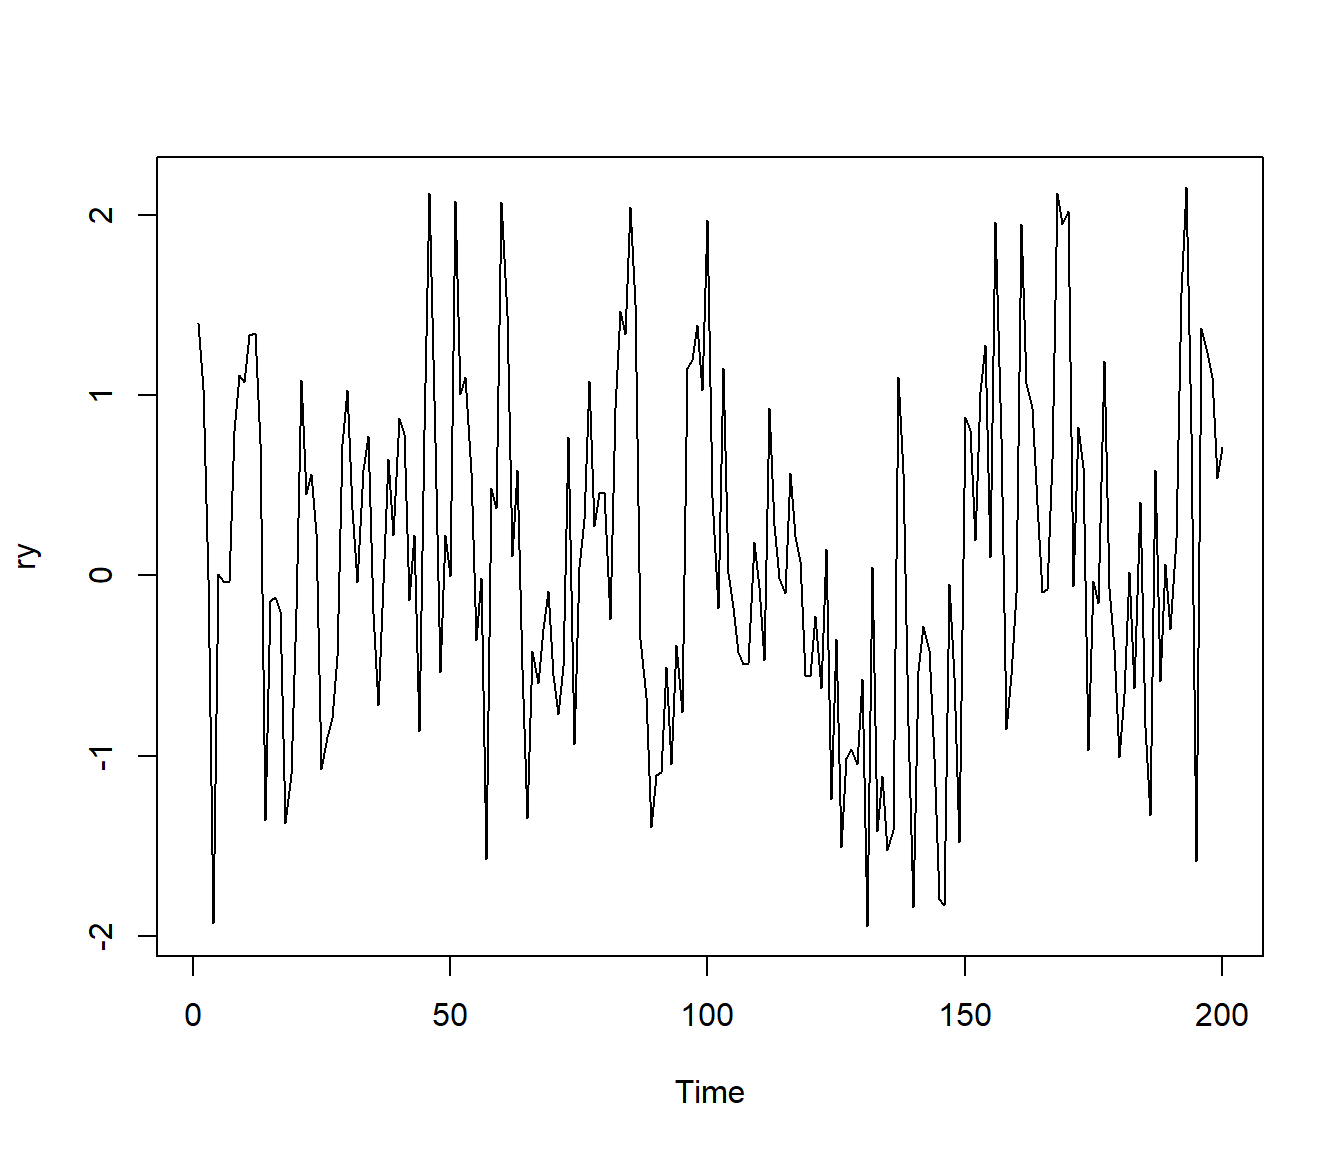
\includegraphics[width=0.7\linewidth]{09-depen_files/figure-latex/arima-sim-1} 

}

\caption{Simulación de un modelo autoregresivo.}\label{fig:arima-sim}
\end{figure}

En este caso el periodo de calentamiento se establece mediante el
parámetro \texttt{n.start} (que se fija automáticamente a un valor
adecuado). La recomendación es fijar la varianza de las series simuladas
si se quieren comparar resultados considerando distintos parámetros de
dependencia.

Otras opciones:

\begin{itemize}
\item
  \texttt{rand.gen\ =\ rnorm}
\item
  \texttt{innov\ =\ rand.gen(n,\ ...)}
\item
  \texttt{n.start\ =\ NA}
\item
  \texttt{start.innov\ =\ rand.gen(n.start,\ ...)}
\end{itemize}

Ejemplo (\texttt{?arima.sim}): {[}Figura \ref{fig:arima-sim2}{]}

\begin{Shaded}
\begin{Highlighting}[]
\NormalTok{ry2 <-}\StringTok{ }\KeywordTok{arima.sim}\NormalTok{(}\DataTypeTok{n =} \DecValTok{63}\NormalTok{, }\KeywordTok{list}\NormalTok{(}\DataTypeTok{ar =} \KeywordTok{c}\NormalTok{(}\FloatTok{0.8897}\NormalTok{, }\OperatorTok{-}\FloatTok{0.4858}\NormalTok{), }
          \DataTypeTok{ma =} \KeywordTok{c}\NormalTok{(}\OperatorTok{-}\FloatTok{0.2279}\NormalTok{, }\FloatTok{0.2488}\NormalTok{)),}
          \DataTypeTok{rand.gen =} \ControlFlowTok{function}\NormalTok{(n, ...) }\KeywordTok{sqrt}\NormalTok{(}\FloatTok{0.1796}\NormalTok{) }\OperatorTok{*}\StringTok{ }\KeywordTok{rt}\NormalTok{(n, }\DataTypeTok{df =} \DecValTok{5}\NormalTok{))}

\KeywordTok{plot}\NormalTok{(ry2)}
\end{Highlighting}
\end{Shaded}

\begin{figure}[!htb]

{\centering 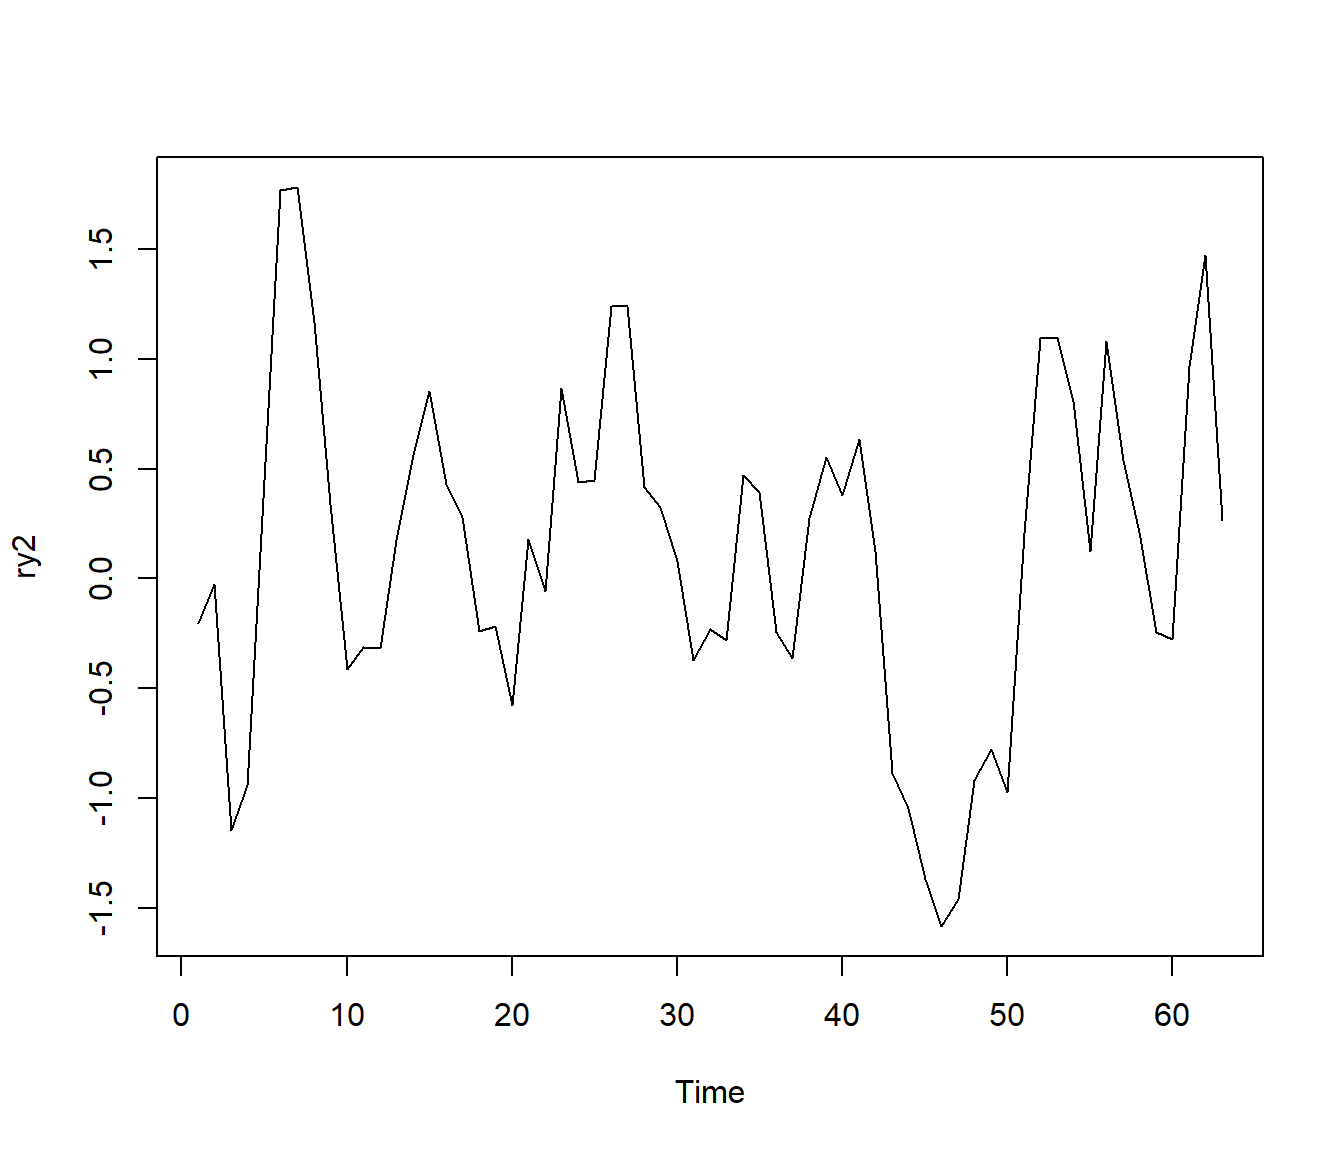
\includegraphics[width=0.7\linewidth]{09-depen_files/figure-latex/arima-sim2-1} 

}

\caption{Simulación de un modelo autoregresivo con errores con distribución *t* de Student.}\label{fig:arima-sim2}
\end{figure}

\section{\texorpdfstring{Implementación en \texttt{R} con el paquete
\texttt{boot}}{Implementación en R con el paquete boot}}\label{implementacion-en-r-con-el-paquete-boot}

La función \texttt{tsboot()} del paquete \texttt{boot} implementa
distintos métodos de remuestreo para series de tiempo.

\begin{Shaded}
\begin{Highlighting}[]
\KeywordTok{library}\NormalTok{(boot)}
\CommentTok{# ?tsboot}
\end{Highlighting}
\end{Shaded}

\subsection{Rnews 1}\label{rnews-1}

Canty, A. J. (2002).
\href{http://cran.fhcrc.org/doc/Rnews/Rnews_2002-3.pdf}{Resampling
methods in R: the boot package}. Rnews: The Newsletter of the R Project,
2 (3), pp.~2-7.

\begin{quote}
``\texttt{tsboot()} can do either of these methods by specifying
\texttt{sim="fixed"} or \texttt{sim="geom"} respectively. A simple call
to tsboot includes the time series, a function for the
\texttt{statistic} (the first argument of this function being the time
series itself), the number of bootstrap replicates, the simulation type
and the (mean) block length''.
\end{quote}

\begin{Shaded}
\begin{Highlighting}[]
\CommentTok{# Datos}
\KeywordTok{data}\NormalTok{(lynx)}
\CommentTok{# ?lynx}
\CommentTok{# Boot}
\KeywordTok{library}\NormalTok{(boot)}
\NormalTok{lynx.fun <-}\StringTok{ }\ControlFlowTok{function}\NormalTok{(tsb) \{}
\NormalTok{  fit <-}\StringTok{ }\KeywordTok{ar}\NormalTok{(tsb, }\DataTypeTok{order.max =} \DecValTok{25}\NormalTok{)}
  \KeywordTok{c}\NormalTok{(fit}\OperatorTok{$}\NormalTok{order, }\KeywordTok{mean}\NormalTok{(tsb)) }
\NormalTok{\}}
\CommentTok{# tsboot}
\KeywordTok{set.seed}\NormalTok{(}\DecValTok{1}\NormalTok{)}
\KeywordTok{tsboot}\NormalTok{(}\KeywordTok{log}\NormalTok{(lynx), lynx.fun, }\DataTypeTok{R =} \DecValTok{199}\NormalTok{, }\DataTypeTok{sim =} \StringTok{"geom"}\NormalTok{, }\DataTypeTok{l =} \DecValTok{20}\NormalTok{)}
\end{Highlighting}
\end{Shaded}

\begin{verbatim}
## 
## STATIONARY BOOTSTRAP FOR TIME SERIES
## 
## Average Block Length of 20 
## 
## Call:
## tsboot(tseries = log(lynx), statistic = lynx.fun, R = 199, l = 20, 
##     sim = "geom")
## 
## 
## Bootstrap Statistics :
##      original       bias    std. error
## t1* 11.000000 -6.216080402   2.8210147
## t2*  6.685933  0.004037546   0.1133995
\end{verbatim}

\subsection{Rnews 2}\label{rnews-2}

Canty, A. J. (2002).
\href{http://cran.fhcrc.org/doc/Rnews/Rnews_2002-3.pdf}{Resampling
methods in R: the boot package}. Rnews: The Newsletter of the R Project,
2 (3), pp.~2-7.

\begin{quote}
``An alternative to the block bootstrap is to use model based
resampling. In this case a model is fitted to the time series so that
the errors are i.i.d. The observed residuals are sampled as an i.i.d.
series and then a bootstrap time series is reconstructed. In
constructing the bootstrap time series from the residuals, it is
recommended to generate a long time series and then discard the initial
burn-in stage. Since the length of burn-in required is problem specific,
\texttt{tsboot} does not actually do the resampling. Instead the user
should give a function which will return the bootstrap time series. This
function should take three arguments, the time series as supplied to
\texttt{tsboot}, a value \texttt{n.sim} which is the length of the time
series required and the third argument containing any other information
needed by the random generation function such as coefficient estimates.
When the random generation function is called it will be passed the
arguments \texttt{data}, \texttt{n.sim} and \texttt{ran.args} passed to
\texttt{tsboot} or their defaults.

One problem with the model-based bootstrap is that it is critically
dependent on the correct model being fitted to the data. Davison and
Hinkley (1997) suggest post-blackening as a compromise between the block
bootstrap and the model-based bootstrap. In this method a simple model
is fitted and the residuals are found. These residuals are passed as the
dataset to \texttt{tsboot} and are resampled using the block (or
stationary) bootstrap. To create the bootstrap time series the resampled
residuals should be put back through the fitted model filter. The
function \texttt{ran.gen} can be used to do this''.
\end{quote}

\begin{Shaded}
\begin{Highlighting}[]
\CommentTok{# Datos}
\NormalTok{lynx1 <-}\StringTok{ }\KeywordTok{log}\NormalTok{(lynx)}
\CommentTok{# Modelo}
\NormalTok{lynx.ar <-}\StringTok{ }\KeywordTok{ar}\NormalTok{(lynx1)}
\CommentTok{# Residuos}
\NormalTok{lynx.res <-}\StringTok{ }\KeywordTok{with}\NormalTok{(lynx.ar, resid[}\OperatorTok{!}\KeywordTok{is.na}\NormalTok{(resid)])}
\NormalTok{lynx.res <-}\StringTok{ }\NormalTok{lynx.res }\OperatorTok{-}\StringTok{ }\KeywordTok{mean}\NormalTok{(lynx.res)}
\CommentTok{# Boot}
\KeywordTok{library}\NormalTok{(boot)}
\NormalTok{lynx.ord <-}\StringTok{ }\KeywordTok{c}\NormalTok{(lynx.ar}\OperatorTok{$}\NormalTok{order, }\DecValTok{0}\NormalTok{, }\DecValTok{0}\NormalTok{)}
\NormalTok{lynx.mod <-}\StringTok{ }\KeywordTok{list}\NormalTok{(}\DataTypeTok{order =}\NormalTok{ lynx.ord, }\DataTypeTok{ar =}\NormalTok{ lynx.ar}\OperatorTok{$}\NormalTok{ar)}
\NormalTok{lynx.args <-}\StringTok{ }\KeywordTok{list}\NormalTok{(}\DataTypeTok{mean =} \KeywordTok{mean}\NormalTok{(lynx1), }\DataTypeTok{model =}\NormalTok{ lynx.mod)}
\NormalTok{lynx.black <-}\StringTok{ }\ControlFlowTok{function}\NormalTok{(res, n.sim, ran.args) \{}
\NormalTok{    m <-}\StringTok{ }\NormalTok{ran.args}\OperatorTok{$}\NormalTok{mean}
\NormalTok{    ts.mod <-}\StringTok{ }\NormalTok{ran.args}\OperatorTok{$}\NormalTok{model}
\NormalTok{    m }\OperatorTok{+}\StringTok{ }\KeywordTok{filter}\NormalTok{(res, ts.mod}\OperatorTok{$}\NormalTok{ar, }\DataTypeTok{method =} \StringTok{"recursive"}\NormalTok{) }
\NormalTok{\}}
\CommentTok{# tsboot}
\KeywordTok{set.seed}\NormalTok{(}\DecValTok{1}\NormalTok{)}
\KeywordTok{tsboot}\NormalTok{(lynx.res, lynx.fun, }\DataTypeTok{R =} \DecValTok{199}\NormalTok{, }\DataTypeTok{l =} \DecValTok{20}\NormalTok{, }
        \DataTypeTok{sim =} \StringTok{"fixed"}\NormalTok{, }\DataTypeTok{n.sim =} \DecValTok{114}\NormalTok{,}
        \DataTypeTok{ran.gen =}\NormalTok{ lynx.black, }\DataTypeTok{ran.args =}\NormalTok{ lynx.args)}
\end{Highlighting}
\end{Shaded}

\begin{verbatim}
## 
## POST-BLACKENED BLOCK BOOTSTRAP FOR TIME SERIES
## 
## Fixed Block Length of 20 
## 
## Call:
## tsboot(tseries = lynx.res, statistic = lynx.fun, R = 199, l = 20, 
##     sim = "fixed", n.sim = 114, ran.gen = lynx.black, ran.args = lynx.args)
## 
## 
## Bootstrap Statistics :
##       original   bias    std. error
## t1* 0.0000e+00 9.954774  3.24628223
## t2* 6.1989e-18 6.678628  0.09172397
\end{verbatim}

\section{Ejercicios}\label{ejercicios-1}

\BeginKnitrBlock{exercise}[Practical 8.1, Lynx data: Davison y Hinkley, 1997]
\protect\hypertarget{exr:tsboot-lynx}{}{\label{exr:tsboot-lynx}
\iffalse (Practical 8.1, Lynx data: Davison y Hinkley, 1997) \fi{} }
Reproducir el ``Practical 8.1 (Lynx data)'' en Davison, A. C., y
Hinkley, D. V. (1997). Bootstrap methods and their application.
Cambridge university press, \url{http://statwww.epfl.ch/davison/BMA}
(\href{http://webcache.googleusercontent.com/search?q=cache:a4nFL5ymMMoJ:statwww.epfl.ch/davison/BMA/+\&cd=1\&hl=gl\&ct=clnk\&gl=es}{caché}):
\EndKnitrBlock{exercise}

\begin{quote}
``Dataframe lynx contains the Canadian lynx data, to the logarithm of
which we fit the autoregressive model that minimizes AIC:
\end{quote}

{[}Figura \ref{fig:lynx-data}{]}

\begin{Shaded}
\begin{Highlighting}[]
\KeywordTok{ts.plot}\NormalTok{(}\KeywordTok{log}\NormalTok{(lynx))}
\end{Highlighting}
\end{Shaded}

\begin{figure}[!htb]

{\centering 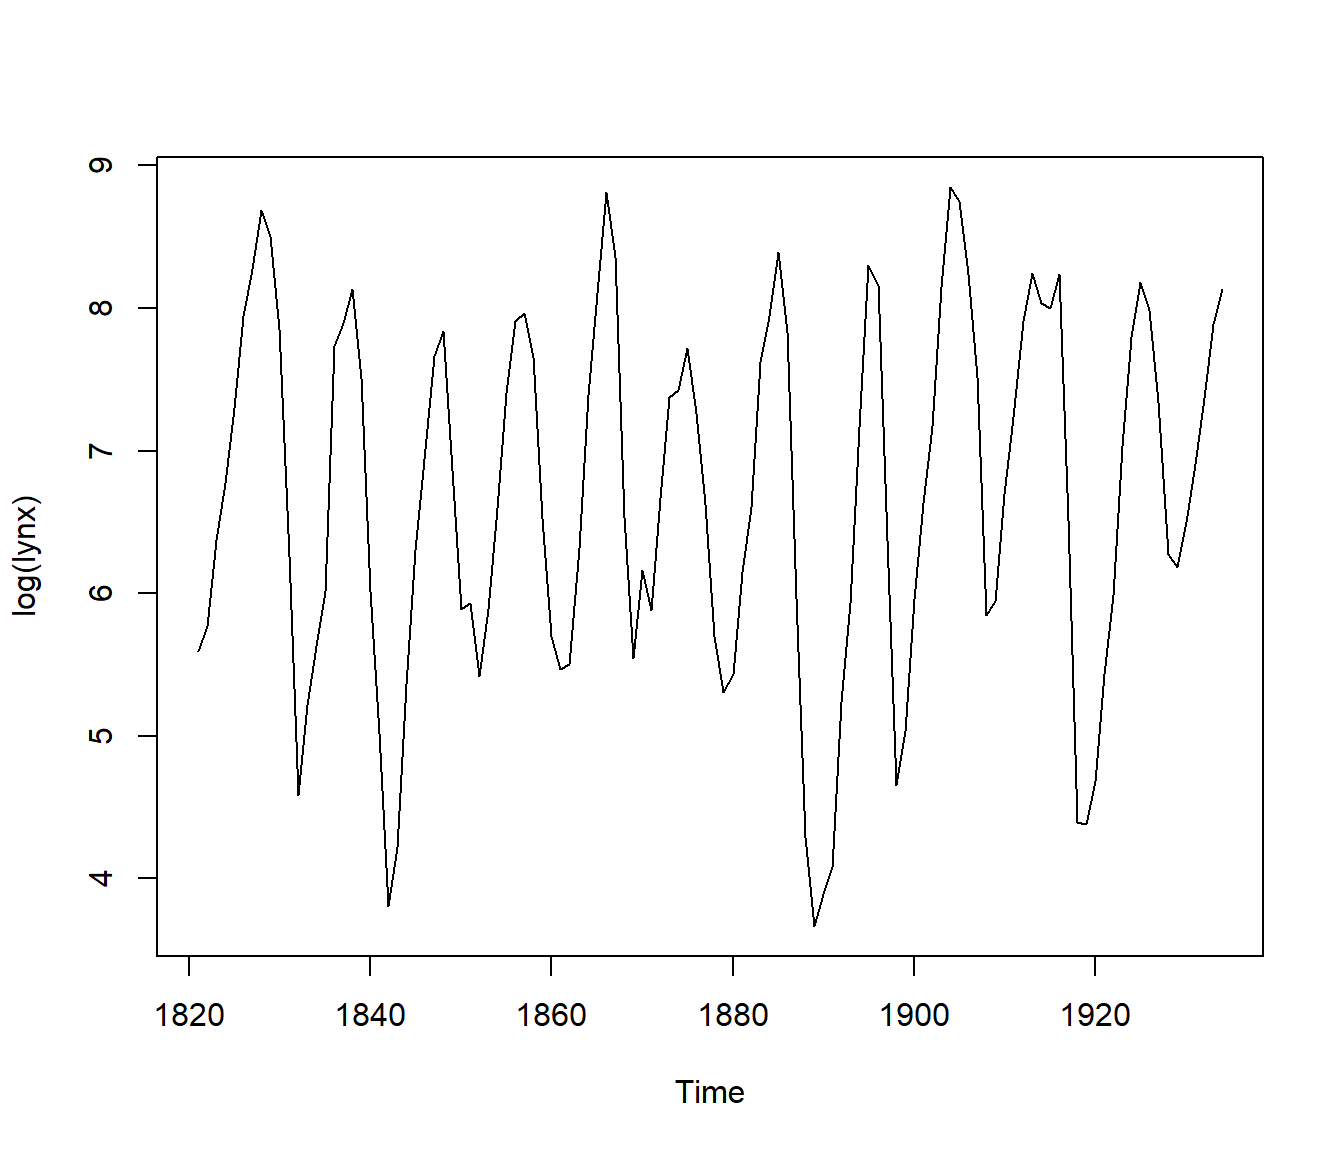
\includegraphics[width=0.7\linewidth]{09-depen_files/figure-latex/lynx-data-1} 

}

\caption{Lynx data (logarithmic scale).}\label{fig:lynx-data}
\end{figure}

\begin{Shaded}
\begin{Highlighting}[]
\NormalTok{lynx.ar <-}\StringTok{ }\KeywordTok{ar}\NormalTok{(}\KeywordTok{log}\NormalTok{(lynx))}
\NormalTok{lynx.ar}\OperatorTok{$}\NormalTok{order}
\end{Highlighting}
\end{Shaded}

\begin{verbatim}
## [1] 11
\end{verbatim}

\begin{quote}
The best model is AR(11). How well determined is this, and what is the
variance of the series average? We bootstrap to see, using
\texttt{lynx.fun} (given below), which calculates the order of the
fitted autoregressive model, the series average, and saves the series
itself.
\end{quote}

\begin{quote}
Here are results for fixed-block bootstraps with block length
\(l = 20\):
\end{quote}

\begin{Shaded}
\begin{Highlighting}[]
\KeywordTok{set.seed}\NormalTok{(DNI)}
\NormalTok{lynx.fun <-}\StringTok{ }\ControlFlowTok{function}\NormalTok{(tsb) \{ }
\NormalTok{  ar.fit <-}\StringTok{ }\KeywordTok{ar}\NormalTok{(tsb, }\DataTypeTok{order.max=}\DecValTok{25}\NormalTok{)}
  \KeywordTok{c}\NormalTok{(ar.fit}\OperatorTok{$}\NormalTok{order, }\KeywordTok{mean}\NormalTok{(tsb), tsb) }
\NormalTok{\}}
\NormalTok{lynx.}\DecValTok{1}\NormalTok{ <-}\StringTok{ }\KeywordTok{tsboot}\NormalTok{(}\KeywordTok{log}\NormalTok{(lynx), lynx.fun, }\DataTypeTok{R=}\DecValTok{99}\NormalTok{, }\DataTypeTok{l=}\DecValTok{20}\NormalTok{, }\DataTypeTok{sim=}\StringTok{"fixed"}\NormalTok{)}
\NormalTok{lynx.}\DecValTok{1}
\KeywordTok{ts.plot}\NormalTok{(}\KeywordTok{ts}\NormalTok{(lynx.}\DecValTok{1}\OperatorTok{$}\NormalTok{t[}\DecValTok{1}\NormalTok{,}\DecValTok{3}\OperatorTok{:}\DecValTok{116}\NormalTok{],}\DataTypeTok{start=}\KeywordTok{c}\NormalTok{(}\DecValTok{1821}\NormalTok{,}\DecValTok{1}\NormalTok{)),}
        \DataTypeTok{main=}\StringTok{"Block simulation, l=20"}\NormalTok{)}
\KeywordTok{boot.array}\NormalTok{(lynx.}\DecValTok{1}\NormalTok{)[}\DecValTok{1}\NormalTok{,]}
\KeywordTok{table}\NormalTok{(lynx.}\DecValTok{1}\OperatorTok{$}\NormalTok{t[,}\DecValTok{1}\NormalTok{])}
\KeywordTok{var}\NormalTok{(lynx.}\DecValTok{1}\OperatorTok{$}\NormalTok{t[,}\DecValTok{2}\NormalTok{])}
\KeywordTok{qqnorm}\NormalTok{(lynx.}\DecValTok{1}\OperatorTok{$}\NormalTok{t[,}\DecValTok{2}\NormalTok{]);}
\KeywordTok{abline}\NormalTok{(}\KeywordTok{mean}\NormalTok{(lynx.}\DecValTok{1}\OperatorTok{$}\NormalTok{t[,}\DecValTok{2}\NormalTok{]),}\KeywordTok{sqrt}\NormalTok{(}\KeywordTok{var}\NormalTok{(lynx.}\DecValTok{1}\OperatorTok{$}\NormalTok{t[,}\DecValTok{2}\NormalTok{])),}\DataTypeTok{lty=}\DecValTok{2}\NormalTok{)}
\end{Highlighting}
\end{Shaded}

\begin{quote}
To obtain similar results for the stationary bootstrap with mean block
length \(l = 20\):
\end{quote}

\begin{Shaded}
\begin{Highlighting}[]
\NormalTok{.Random.seed <-}\StringTok{ }\NormalTok{lynx.}\DecValTok{1}\OperatorTok{$}\NormalTok{seed}
\NormalTok{lynx.}\DecValTok{2}\NormalTok{ <-}\StringTok{ }\KeywordTok{tsboot}\NormalTok{(}\KeywordTok{log}\NormalTok{(lynx), lynx.fun, ...}
\CommentTok{# lynx.2}
\end{Highlighting}
\end{Shaded}

\begin{quote}
See if the results look different from those above. Do the simulated
series using blocks look like the original? Compare the estimated
variances under the two resampling schemes. Try different block lengths,
and see how the variances of the series average change.
\end{quote}

\begin{quote}
For model-based resampling we need to store results from the original
model:
\end{quote}

\begin{quote}
Check the orders of the fitted models for this scheme.
\end{quote}

\begin{quote}
For post-blackening we need to define yet another function:
\end{quote}

\begin{quote}
Compare these results with those above, and try the post-blackened
bootstrap with \texttt{sim="geom"}. (Sections 8.2.2, 8.2.3)''.
\end{quote}

\BeginKnitrBlock{exercise}[Practical 8.2, Beaver data: Davison y Hinkley, 1997]
\protect\hypertarget{exr:tsboot-beaver}{}{\label{exr:tsboot-beaver}
\iffalse (Practical 8.2, Beaver data: Davison y Hinkley, 1997) \fi{} }
Reproducir el ``Practical 8.2 (Beaver data)'' en Davison, A. C., y
Hinkley, D. V. (1997). Bootstrap methods and their application.
Cambridge university press, \url{http://statwww.epfl.ch/davison/BMA}
(\href{http://webcache.googleusercontent.com/search?q=cache:a4nFL5ymMMoJ:statwww.epfl.ch/davison/BMA/+\&cd=1\&hl=gl\&ct=clnk\&gl=es}{caché}):
\EndKnitrBlock{exercise}

\begin{quote}
``The data in beaver consist of a time series of \(n = 100\)
observations on the body temperature \(y_1, \ldots, y_n\) and an
indicator \(x_1, \ldots, x_n\) of activity of a female beaver, Castor
canadensis.
\end{quote}

{[}Figura \ref{fig:beaver-data}{]}

\begin{Shaded}
\begin{Highlighting}[]
\CommentTok{# ?beaver}
\KeywordTok{plot}\NormalTok{(beaver)}
\end{Highlighting}
\end{Shaded}

\begin{figure}[!htb]

{\centering 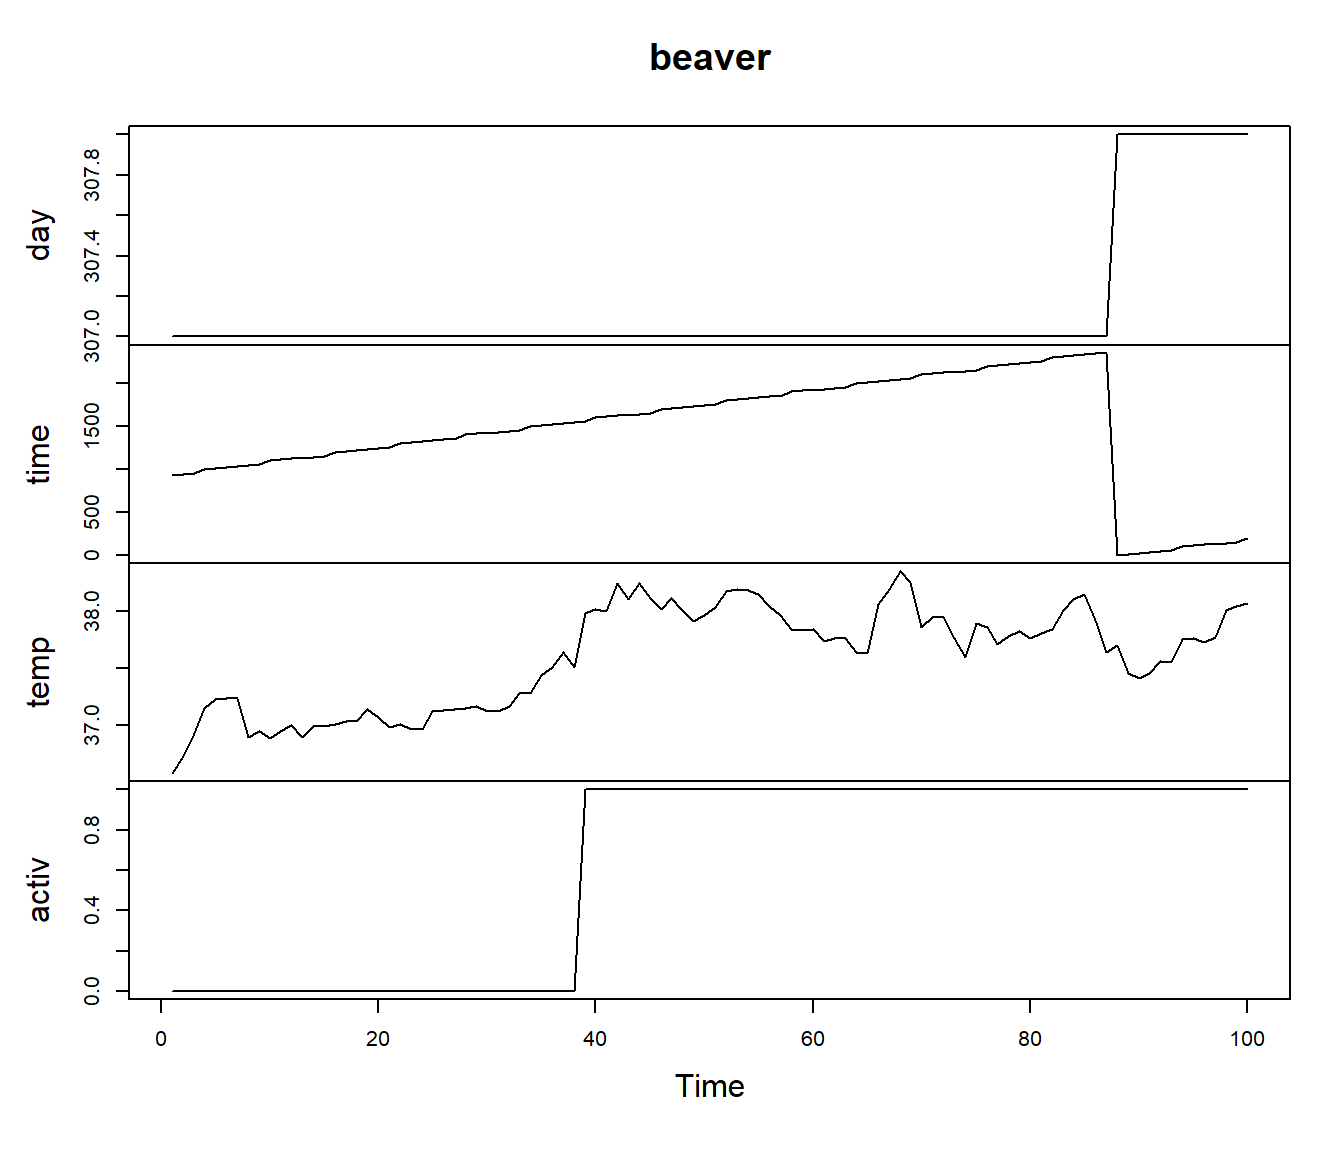
\includegraphics[width=0.7\linewidth]{09-depen_files/figure-latex/beaver-data-1} 

}

\caption{Beaver data}\label{fig:beaver-data}
\end{figure}

\begin{Shaded}
\begin{Highlighting}[]
\KeywordTok{class}\NormalTok{(beaver)}
\end{Highlighting}
\end{Shaded}

\begin{verbatim}
## [1] "mts" "ts"
\end{verbatim}

\begin{Shaded}
\begin{Highlighting}[]
\KeywordTok{str}\NormalTok{(beaver) }
\end{Highlighting}
\end{Shaded}

\begin{verbatim}
##  Time-Series [1:100, 1:4] from 1 to 100: 307 307 307 307 307 307 307 307 307 307 ...
##  - attr(*, "dimnames")=List of 2
##   ..$ : NULL
##   ..$ : chr [1:4] "day" "time" "temp" "activ"
\end{verbatim}

\begin{quote}
We want to estimate and give an uncertainty measure for the body
temperature of the beaver. The simplest model that allows for the clear
autocorrelation of the series is \ldots{}
\end{quote}

\begin{quote}
To fit the original model and to generate a new series:
\end{quote}

\begin{Shaded}
\begin{Highlighting}[]
\NormalTok{data <-}\StringTok{ }\NormalTok{beaver}
\CommentTok{# fit <- function( data )\{ }
\CommentTok{#   #  X <- cbind(rep(1,100),data$activ) # ErrorR}
\CommentTok{#   X <- cbind(rep(1, 100), data[,"activ"])}
\CommentTok{#   para <- list(X = X, data = data)}
\CommentTok{#   # assign("para",para, frame=1) # ErrorR}
\CommentTok{#   # assign("para", para, envir = .GlobalEnv)}
\CommentTok{#   para <<- para}
\CommentTok{#   # arima.mle # ErrorR}
\CommentTok{# ----------------------------}
\CommentTok{#   d <- arima.mle(x = para$data$temp,}
\CommentTok{#               model = list(ar = c(0.8)), xreg = para$X)}
\CommentTok{#   res <- arima.diag(d, plot = F, std.resid = T)$std.resid}
\CommentTok{#   res <- res[!is.na(res)]}
\CommentTok{#   list(}
\CommentTok{#     paras = c(d$model$ar, d$reg.coef, sqrt(d$sigma2)),}
\CommentTok{#     res = res - mean(res),}
\CommentTok{#     fit = X %*% d$reg.coef)  }
\CommentTok{# \}}
\CommentTok{# }
\CommentTok{# beaver.args <- fit(beaver)}
\CommentTok{# white.noise <- function(n.sim, ts) }
\CommentTok{#     sample(ts, size = n.sim, replace = TRUE)}
\CommentTok{# beaver.gen <- function(ts, n.sim, ran.args)\{}
\CommentTok{#     tsb <- ran.args$res}
\CommentTok{#     fit <- ran.args$fit}
\CommentTok{#     coeff <- ran.args$paras}
\CommentTok{#     ts$temp <- fit + coeff[4] * arima.sim(model = list(ar = coeff[1]),}
\CommentTok{#         n = n.sim, rand.gen = white.noise, ts = tsb)}
\CommentTok{#     ts}
\CommentTok{# \}}
\CommentTok{# new.beaver <- beaver.gen( beaver, 100, beaver.args )}
\end{Highlighting}
\end{Shaded}

\begin{quote}
Now we are able to generate data, we can bootstrap and see the results
of \texttt{beaver.boot} as follows:
\end{quote}

\begin{Shaded}
\begin{Highlighting}[]
\CommentTok{# beaver.fun <- function(ts) fit(ts)$paras}
\CommentTok{# beaver.boot <- tsboot( beaver, beaver.fun, R=99,sim="model", }
\CommentTok{#         n.sim=100,ran.gen=beaver.gen,ran.args=beaver.args) }
\CommentTok{# names(beaver.boot)}
\CommentTok{# beaver.boot$t0}
\CommentTok{# beaver.boot$t[1:10,]}
\end{Highlighting}
\end{Shaded}

\begin{quote}
showing the original value of \texttt{beaver.fun} and its value for the
first 10 replicate series. Are the estimated mean temperatures for the
\texttt{R\ =\ 99} simulations normal? Use \texttt{boot.ci} to obtain
normal and basic bootstrap confidence intervals for the resting and
active temperatures. In this analysis we have assumed that the linear
model with AR(1) errors is appropriate. How would you proceed if it were
not? (Section 8.2; Reynolds, 1994)''.
\end{quote}

\BeginKnitrBlock{exercise}[Practical 8.3, Sunspot data: Davison y Hinkley, 1997]
\protect\hypertarget{exr:tsboot-sunspot}{}{\label{exr:tsboot-sunspot}
\iffalse (Practical 8.3, Sunspot data: Davison y Hinkley, 1997) \fi{} }
Reproducir el ``Practical 8.3 (Sunspot data)'' en Davison, A. C., y
Hinkley, D. V. (1997). Bootstrap methods and their application.
Cambridge university press, \url{http://statwww.epfl.ch/davison/BMA}
(\href{http://webcache.googleusercontent.com/search?q=cache:a4nFL5ymMMoJ:statwww.epfl.ch/davison/BMA/+\&cd=1\&hl=gl\&ct=clnk\&gl=es}{caché}):
\EndKnitrBlock{exercise}

\begin{quote}
``Consider scrambling the phases of the sunspot data. To see the
original data,
\end{quote}

{[}Figura \ref{fig:sunspot}{]}

\begin{Shaded}
\begin{Highlighting}[]
\KeywordTok{data}\NormalTok{(sunspot.year)  }\CommentTok{# WarningR: data set 'sunspot' not found}
\CommentTok{# ?sunspot.year}
\NormalTok{yl <-}\StringTok{ }\KeywordTok{c}\NormalTok{(}\OperatorTok{-}\DecValTok{50}\NormalTok{, }\DecValTok{200}\NormalTok{)}
\KeywordTok{plot}\NormalTok{(sunspot.year, }\DataTypeTok{ylim =}\NormalTok{ yl)}
\KeywordTok{abline}\NormalTok{(}\DataTypeTok{h =} \DecValTok{0}\NormalTok{, }\DataTypeTok{lty =} \DecValTok{2}\NormalTok{)}
\end{Highlighting}
\end{Shaded}

\begin{figure}[!htb]

{\centering 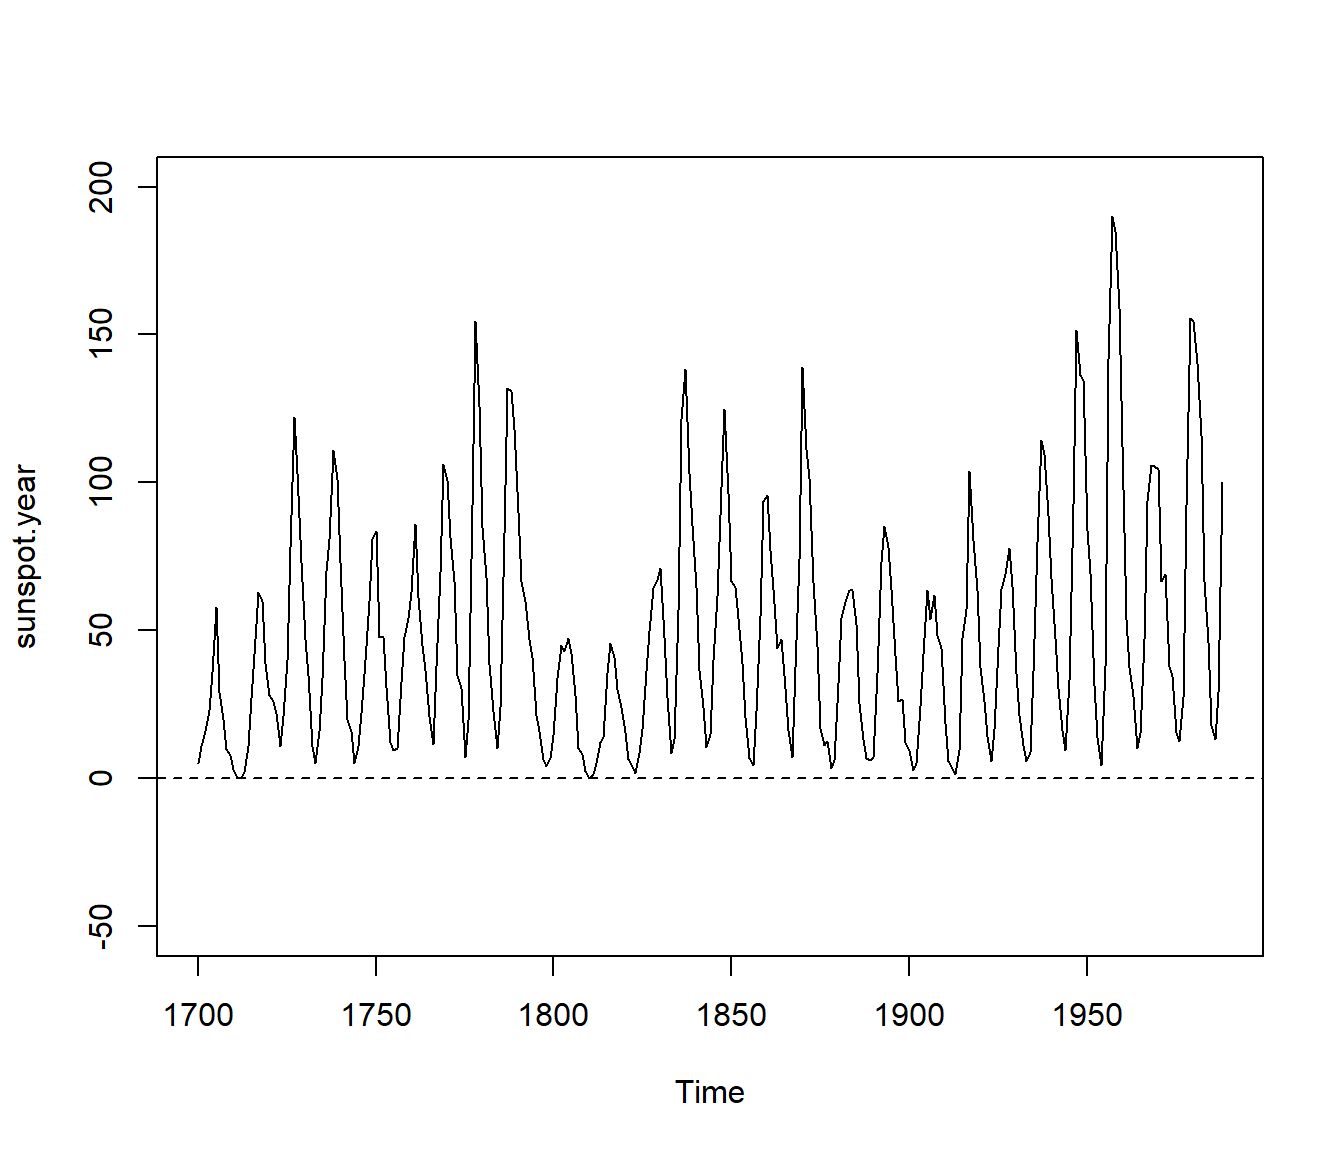
\includegraphics[width=0.7\linewidth]{09-depen_files/figure-latex/sunspot-1} 

}

\caption{Sunspot data (yearly numbers).}\label{fig:sunspot}
\end{figure}

\begin{quote}
two replicates generated using ordinary phase scrambling, and two phase
scrambled series whose marginal distribution is the same as that of the
original data:
\end{quote}

\begin{Shaded}
\begin{Highlighting}[]
\KeywordTok{set.seed}\NormalTok{(DNI)}
\NormalTok{sunspot.}\DecValTok{1}\NormalTok{ <-}\StringTok{ }\KeywordTok{tsboot}\NormalTok{(sunspot.year, ...}
\NormalTok{.Random.seed <-}\StringTok{ }\NormalTok{sunspot.}\DecValTok{1}\OperatorTok{$}\NormalTok{seed }\CommentTok{# set.seed(DNI)}
\NormalTok{sunspot.}\DecValTok{2}\NormalTok{ <-}\StringTok{ }\KeywordTok{tsboot}\NormalTok{(sunspot.year, ...}
\end{Highlighting}
\end{Shaded}

\begin{quote}
What features of the original data are preserved by the two algorithms?
(You may find it helpful to experiment with different shapes for the
figures.) (Section 8.2.4; Problem 8.4; Theiler et al, 1992)''.
\end{quote}

\section{\texorpdfstring{Implementación en \texttt{R} con el paquete
\texttt{forecast}}{Implementación en R con el paquete forecast}}\label{implementacion-en-r-con-el-paquete-forecast}

\subsection{Bootstrap condicional (a partir de un modelo
ajustado)}\label{bootstrap-condicional-a-partir-de-un-modelo-ajustado}

En la práctica normalmente se ajusta un modelo a los datos observados y
posteriormente se obtienen las simulaciones condicionadas empleando el
modelo ajustado.

Por ejemplo, en el caso de series de tiempo, se puede emplear la función
\texttt{simulate} del paquete \texttt{forecast}: {[}Figura
\ref{fig:co2}{]}

\begin{Shaded}
\begin{Highlighting}[]
\KeywordTok{library}\NormalTok{(forecast)}
\CommentTok{# ?co2}
\NormalTok{data <-}\StringTok{ }\KeywordTok{window}\NormalTok{(co2, }\DecValTok{1990}\NormalTok{) }\CommentTok{# datos de co2 desde 1990 (hasta 1997)}
\KeywordTok{plot}\NormalTok{(data, }\DataTypeTok{ylab =} \KeywordTok{expression}\NormalTok{(}\StringTok{"Atmospheric concentration of CO"}\NormalTok{[}\DecValTok{2}\NormalTok{]), }
     \DataTypeTok{xlim=}\KeywordTok{c}\NormalTok{(}\DecValTok{1990}\NormalTok{,}\DecValTok{2000}\NormalTok{), }\DataTypeTok{ylim=}\KeywordTok{c}\NormalTok{(}\DecValTok{350}\NormalTok{, }\DecValTok{375}\NormalTok{))}
\NormalTok{data2 <-}\StringTok{ }\KeywordTok{window}\NormalTok{(co2, }\DecValTok{1990}\NormalTok{, }\DecValTok{1996}\NormalTok{) }\CommentTok{# datos de co2 desde 1990 hasta 1996}
\NormalTok{fit <-}\StringTok{ }\KeywordTok{ets}\NormalTok{(data2)}
\CommentTok{# Simulación condicional}
\KeywordTok{set.seed}\NormalTok{(}\DecValTok{1}\NormalTok{)}
\NormalTok{ry <-}\StringTok{ }\KeywordTok{simulate}\NormalTok{(fit, }\DecValTok{12}\OperatorTok{*}\DecValTok{4}\NormalTok{)}
\KeywordTok{lines}\NormalTok{(ry, }\DataTypeTok{col=}\StringTok{"red"}\NormalTok{)}
\end{Highlighting}
\end{Shaded}

\begin{figure}[!htb]

{\centering 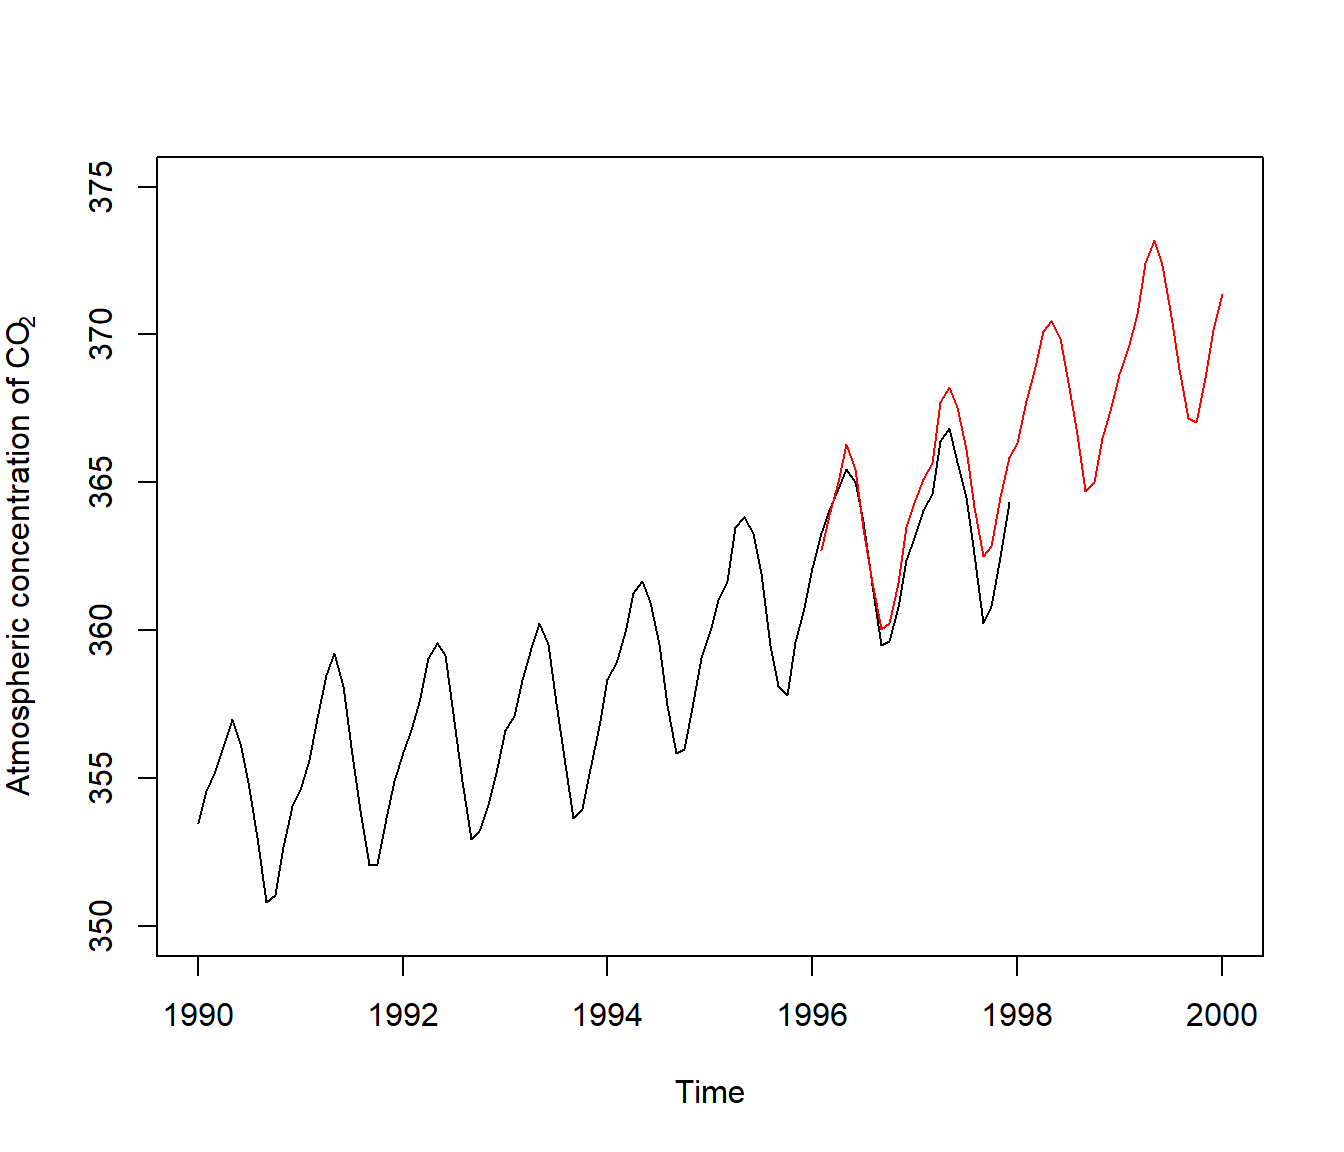
\includegraphics[width=0.7\linewidth]{09-depen_files/figure-latex/co2-1} 

}

\caption{Datos de co2 (1990-1997) y simulación condicional (a partir de las observaciones desde 1990 hasta 1996).}\label{fig:co2}
\end{figure}

\begin{Shaded}
\begin{Highlighting}[]
\KeywordTok{plot}\NormalTok{(}\KeywordTok{forecast}\NormalTok{(fit, }\DataTypeTok{h=}\DecValTok{12}\OperatorTok{*}\DecValTok{4}\NormalTok{), }\DataTypeTok{col=}\StringTok{"blue"}\NormalTok{)}
\KeywordTok{lines}\NormalTok{(ry, }\DataTypeTok{col=}\StringTok{"red"}\NormalTok{)}
\end{Highlighting}
\end{Shaded}

\begin{figure}[!htb]

{\centering 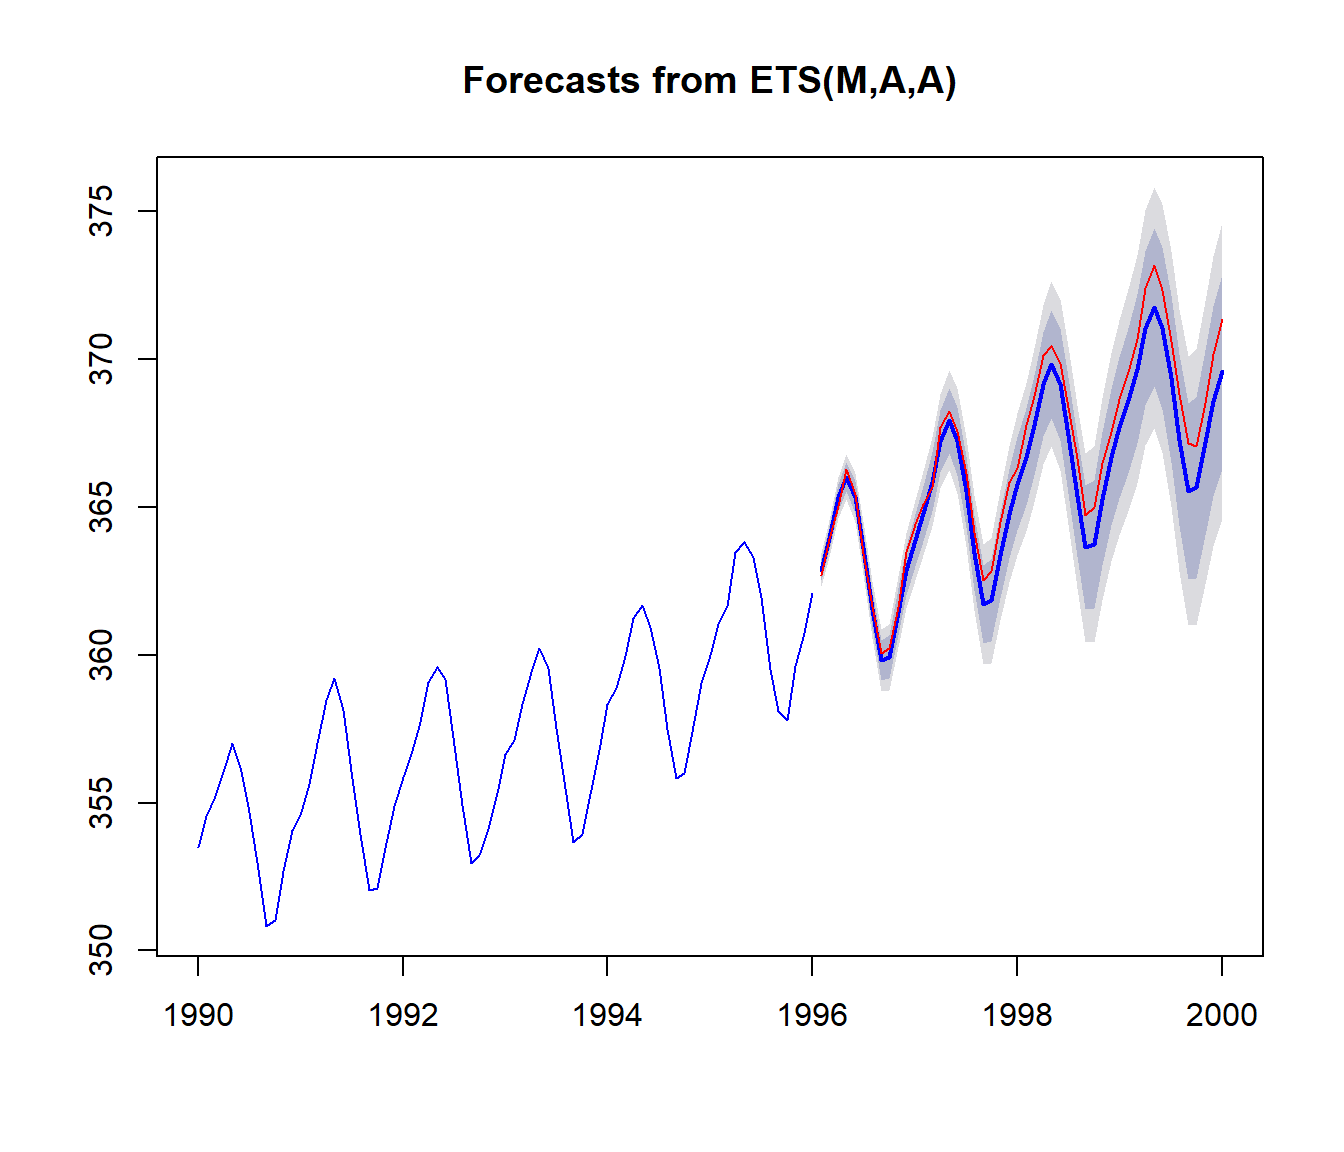
\includegraphics[width=0.7\linewidth]{09-depen_files/figure-latex/co22-1} 

}

\caption{Predicción de los valores de co2 y simulación condicional (ambas a partir de las observaciones entre 1990 y 1996).}\label{fig:co22}
\end{figure}

{[}Figura \ref{fig:co22}{]}

Ver enlaces en apéndice \ref{forecast-links}.

\section{Spatial data}\label{spatial-data}

Ver enlaces en apéndice \ref{spatial-links}.

\chapter*{Referencias}\label{referencias}
\addcontentsline{toc}{chapter}{Referencias}

Akritas, M. G. (1986).
\href{https://www.tandfonline.com/doi/abs/10.1080/01621459.1986.10478369}{Bootstrapping
the Kaplan--Meier estimator}. \emph{J. Amer. Stat. Assoc.} \textbf{81},
1032--1038.

Beran, R. (1987). Prepivoting to reduce level error of confidence sets.
\emph{Biometrika} \textbf{74}, 457-468.

Bhattacharya, R.N. and Ghosh, J.K. (1978). On the validity of the formal
Edgeworth expansion. \emph{Ann. Statist.} \textbf{6}, 434--451.

Bickel, P.J. and Freedman, D.A. (1981). Some Asymptotic theory for the
bootstrap. \emph{Ann. Statist.} \textbf{12} 2, 470-482.

Bowman, A., Hall, P. and Prvan, T. (1998). Bandwidth selection for the
smoothing of distribution functions. \emph{Biometrika} \textbf{85} 4,
799-808.

Breslow, N. and Crowley, J. (1974). A large sample study of the life
table and product limit estimates under random censorship. \emph{Ann.
Statist.} \textbf{2}, 437--453.

Bühlmann, P. (1994). Blockwise bootstrap empirical processes for
stationary sequences. \emph{Ann. Statist.} \textbf{22}, 995-1012.

Bühlmann, P. (1997). Sieve bootstrap for time series. \emph{Bernoulli}
\textbf{3}, 123-148.

Bühlmann, P. (1998). Sieve bootstrap for smoothing in nonstationary time
series. \emph{Ann. Statist.} \textbf{26}, 48-83.

Canty, A. J. (2002).
\href{http://cran.fhcrc.org/doc/Rnews/Rnews_2002-3.pdf}{Resampling
methods in R: the boot package}. \emph{The Newsletter of the R Project}
\textbf{2}, 2-7.

Cao, R. (1990). Órdenes de convergencia para las aproximaciones normal y
bootstrap en la estimación no paramétrica de la función de densidad.
\emph{Trabajos de Estadística}, vol. \textbf{5}, 2, 23-32.

Cao, R. (1991). Rate of convergence for the wild bootstrap in
nonparametric regression. \emph{Ann. Statist} \textbf{19}, 2226-2231.

Cao, R. (1993). Bootstrapping the mean integrated squared error.
\emph{Jr. Mult. Anal.} \textbf{45}, 137--160.

Cao, R. (1999). An overview of bootstrap methods for estimating and
predicting in time series. \emph{Test} \textbf{8}, 95-116.

Cao, R., Cuevas, A. and González-Manteiga, W. (1993). A comparative
study of several smoothing methods in density estimation. \emph{Comp.
Statist. Data Anal.} \textbf{17}, 153--176.

Cao, R., Febrero-Bande, M., González-Manteiga, W., Prada-Sánchez, J.M.
and García-Jurado, I. (1997). Saving computer time in constructing
consistent bootstrap prediction intervals for autoregressive processes.
\emph{Commun. Statist. Simula.} \textbf{26}, 961-978.

Cao, R. and González-Manteiga, W. (1993). Bootstrap methods in
regression smoothing. \emph{Journal of Nonparametric Statistics}
\textbf{2}, 379-388.

Cao, R. and Prada-Sánchez, J.M. (1993). Bootstrapping the mean of a
symmetric population. \emph{Statistics \& Probability Letters}
\textbf{17}, 43-48.

Castillo-Páez, S., Fernández-Casal, R. and García-Soidán, P. (2019).
\href{https://www.sciencedirect.com/science/article/pii/S0167947319300325?via\%3Dihub}{A
nonparametric bootstrap method for spatial data}, \emph{Computational
Statistics and Data Analysis} \textbf{137}, 1-15.

Carlstein, E., Do, K. A., Hall, P., Hesterberg, T., and Künsch, H. R.
(1998).
\href{https://projecteuclid.org/euclid.bj/1174324983}{Matched-block
bootstrap for dependent data .} \emph{Bernoulli} \textbf{4} 3, 305-328.

Cox, D. R. (1972).
\href{https://rss.onlinelibrary.wiley.com/doi/abs/10.1111/j.2517-6161.1972.tb00899.x}{Regression
Models and Life Tables} (with discussion), \emph{Journal of the Royal
Statistical Society series B} \textbf{34}, 187--220.

Davison, A.C. and Hinkley, D.V. (1997). \emph{Bootstrap Methods and
their Application}. Cambridge University Press.

Efron, B. (1979). Bootstrap Methods: Another look at the Jackknife.
\emph{Ann. Statist.} \textbf{7}, 1-26.

Efron, B. (1981). Censored data and the bootstrap. \emph{J. Amer.
Statist. Assoc.} \textbf{76}, 312--319.

Efron, B. (1982). The Jackknife, the Bootstrap and other Resampling
Plans. CBMS-NSF. \emph{Regional Conference series in applied
mathematics}.

Efron, B. (1983). Estimating the error rate of a prediction rule:
improvements on cross-validation. \emph{J. Amer. Stat. Assoc.}
\textbf{78}, 316-331.

Efron, B. (1987). Better Bootstrap confidence intervals (with
discussion). \emph{J. Amer. Stat. Assoc.} \textbf{82}, 171-200.

Efron, B. (1990). More Efficient Bootstrap Computations. \emph{J. Amer.
Statist. Assoc.} \textbf{85}, 79-89.

Efron, B. and Tibshirani, R. (1986). Bootstrap methods for standard
errors, confidence intervals, and other measures of statistical
accuracy. \emph{Statistical Science} \textbf{1}, 54-77.

Efron, B. and Tibshirani, R.J. (1993). \emph{An Introduction to the
Bootstrap}. Chapman and Hall.

Faraway, J.J. and Jhun, M. (1990). Bootstrap choice of bandwidth for
density estimation. \emph{Jr. Amer. Statist. Assoc.} \textbf{85},
1119--1122.

Ferretti, N. and Romo, J. (1996). Unit root bootstrap test for AR(1)
models. \emph{Biometrika} \textbf{83}, 849-860.

Freedman, D.A. (1981). Bootstrapping regression models. \emph{Ann.
Statis.} \textbf{9} 6, 118-1228.

Fuller, W.A. (1976). \emph{Introduction to statistical time series}. New
York: Wiley.

Gannoun, A. (1990). Estimation non paramétrique de la médiane
conditionnelle. Application à la prévision. \emph{C. R. Acad. Sci.
Paris} \textbf{310}, 295-298.

García-Jurado, I. González-Manteiga, W., Prada-Sánchez, J.M.,
Febrero-Bande, M. and Cao, R. (1995). Predicting using Box-Jenkins,
nonparametric and bootstrap techniques. \emph{Technometrics}
\textbf{37}, 303-310.

González-Manteiga, W. and Prada-Sánchez, J.M. (1985). Una aplicación de
los métodos de suavización no paramétricos en la técnica bootstrap.
\emph{Proceedings Jornadas Hispano-Lusas de Matemáticas}. Murcia, 1985.

González-Manteiga, W., Prada-Sánchez, J.M. and Romo, J. (1994). The
Bootstrap-A Review. \emph{Computational Statistics} \textbf{9}, 165-205.

Hall, P. (1986). On the bootstrap and confidence intervals. \emph{Ann.
Statist.} \textbf{14}, 1431-1452.

Hall, P. (1988-a) Theoretical comparison of bootstrap confidence
intervals. \emph{Ann. Statist.} \textbf{16}, 927-953.

Hall, P. (1988-b). Rate of convergence in bootstrap approximations.
\emph{Ann. Probab.} \textbf{16} 4, 1665-1684.

Hall, P. (1990). Using the bootstrap to estimate mean squared error and
select smoothing parameter in nonparametric problems. \emph{J.
Multivariate Anal.} \textbf{32}, 177--203.

Hall. P. (1992).
\href{https://books.google.es/books?hl=es\&lr=\&id=CwLaBwAAQBAJ\&oi=fnd\&pg=PR11\&dq=The+Bootstrap+and+Edgeworth+Expansion}{\emph{The
Bootstrap and Edgeworth Expansion}}. Springer Verlag.

Hall, P., Horowitz, J.L. and Jing, B-Y. (1995). On blocking rules for
the bootstrap with dependent data. \emph{Biometrika} \textbf{82},
561-574.

Hall, P., Marron, J.S. and Park, B. (1992). Smoothed cross-validation.
\emph{Probab. Theor. Rel. Fields} \textbf{92}, 1--20.

Hall, P. and Martin, M.A. (1988). On bootstrap resampling and iteration.
\emph{Biometrika} \textbf{75}, 661-671.

Härdle, W. and Mammen, E. (1993). Comparing nonparametric versus
parametric regression fits. \emph{Ann. Statist.} \textbf{21}, 1926-1947.

Härdle, W. and Marron, J. S. (1991). Bootstrap simultaneous error bars
for nonparametric regression. \emph{Ann. Statist.} \textbf{19},
778--796.

Hartigan, J.A. (1969). Using subsample values as typical values. J.
\emph{Amer. Statist. Assoc.} \textbf{64}, 1303-1317.

Heimann, G. and Kreiss, J-P. (1996). Bootstrapping general first order
autoregression. \emph{Statist. Prob. Lett.} \textbf{30}, 87-98.

Kaplan, E. L. and P. Meier, Nonparametric estimation from incomplete
observations, \emph{J. Amer. Stat. Assoc.} \textbf{53} (1958) 457--481.

Kreiss, J-P. and Franke, J. (1992). Bootstrapping stationary
autoregressive moving average models. \emph{J. Time Ser. Anal.}
\textbf{13}, 297-317.

Künsch, H.R. (1989). The jackknife and the bootstrap for general
stationary observations. \emph{Ann. Statist.} \textbf{17}, 1217-1241.

Liu, R.Y. and Singh, K. (1992). Moving blocks jackknife and bootstrap
capture weak dependence. In
\href{https://books.google.es/books?hl=es\&lr=\&id=ZJzIpNZNVLgC\&oi=fnd\&pg=PA3\&dq=Exploring+the+limits+of+the+bootstrap}{\emph{Exploring
the limits of bootstrap}} (R. LePage and L Billard, Eds.), pp.~225-248.
New York: Wiley.

Mammen, E. (1992).
\href{https://books.google.es/books?hl=es\&lr=\&id=zpDfBwAAQBAJ\&oi=fnd\&pg=PP8\&dq=When+does+Bootstrap+Work\%3F}{\emph{When
does Bootstrap Work?}}. Springer Verlag.

Maritz, J.S. (1979). A note on exact robust confidence intervals for
location. \emph{Biometrika} \textbf{66}, 163-166.

Marron, J.S. (1992). Bootstrap bandwidth selection. In \emph{Exploring
the limits of the bootstrap}, LePage, R. and Billard, L. eds.,
pp.~249--262. New York: Wiley.

Nadaraya, E.A. (1964). On estimating regression. \emph{Theor. Probab.
Appl.} \textbf{9,} 141-142.

Naik-Nimbalkar, U.V. and Rajarshi, M.B. (1994). Validity of blockwise
bootstrap for empirical processes with stationary observations.
\emph{Ann. Statist.} \textbf{22}, 980-994.

Navidi, W. (1989). Edgeworth expansions for bootstrapping regression
models. \emph{Ann. Statist.} \textbf{17} 4, 1472-1478.

Paparoditis, E. (1996). Bootstrapping autoregressive and moving average
parameters estimates of infinite order vector autoregressive processes.
\emph{J. Mult. Anal.} \textbf{57}, 277-296.

Parzen, E. (1962). On estimation of a probability density function and
mode. \emph{Ann. Math. Statist.} \textbf{33}, 1065--1076.

Pascual, L., Romo, J. and Ruiz, E. (2001). Effects of parameter
estimation on prediction densities: a bootstrap approach. \emph{Int. J.
Forecasting} \textbf{17}, 83-103

Politis, D.N. and Romano, J.R. (1994a). The stationary bootstrap.
\emph{J. Amer. Statist. Assoc.} \textbf{89}, 1303-1313.

Politis, D.N. and Romano, J.R. (1994b). Large sample confidence regions
based on subsamples under minimal assumptions. \emph{Ann. Statist.}
\textbf{22}, 2031-2050.

Politis, D.N. and Romano, J.R. (1994c). Limit theorems for weakly
dependent Hilbert space valued random variables with application to the
stationary bootstrap. \emph{Statist. Sin.} \textbf{4}, 461-476.

Politis, D.N., Romano, J.P. and Wolf, M. (1999).
\href{https://books.google.es/books?hl=es\&lr=\&id=nGu6rqjE6JoC\&oi=fnd\&pg=PR7\&dq=Subsampling}{\emph{Subsampling}}.
Springer Verlag.

Prada-Sánchez, J.M. and Cotos-Yáñez, T. (1997). A Simulation Study of
Iterated and Non-iterated Bootstrap Methods for Bias Reduction and
Confidence Interval Estimation. \emph{Comm. Statist .-Simula.}
\textbf{26} 3, 927-946.

Prada-Sánchez, J.M. and Otero-Cepeda, X.L. (1989). The use of smooth
bootstrap techniques for estimating the error rate of a prediction rule.
\emph{Comm. Statist .-Simula.} \textbf{18} 3, 1169-1186.

Quenouille, M. (1949). Approximate test of correlation in time series.
\emph{J. Roy. Statist. Soc. Ser. B} \textbf{11}, 18-84.

Radulović, D. (1996). The bootstrap for the mean of strong mixing
sequences under minimal conditions. \emph{Statist. Prob. Lett.}
\textbf{28}, 65-72.

Reid, N. (1981). Estimating the median survival time. \emph{Biometrika}
\textbf{68}, 601--608.

Rizzo, M.L. (2008). \emph{Statistical Computing with R}.
Chapman\&Hall/CRC

Rosenblatt, M. (1956). Remarks on some nonparametric estimate of a
density function. \emph{Ann. Math. Statist.} \textbf{27}, 832--837.

Rubin, D.B. (1981). The Bayesian Bootstrap. \emph{Ann. Statist.}
\textbf{9} 1, 130-134.

Rubinstein, R.Y. (1981).
\href{https://books.google.es/books?hl=es\&lr=\&id=r2VODQAAQBAJ\&oi=fnd\&pg=PR1\&dq=Simulation+and+the+Monte+Carlo+Method}{\emph{Simulation
and the Monte Carlo Method}}. Wiley.

Schucany, W., Gray, H. and Owen, O. (1971). On bias reduction in
estimation. \emph{J. Amer. Stat. Assoc.} \textbf{66}, 524-533.

Shao, J. (1999).
\href{https://www.springer.com/gp/book/9780387953823}{\emph{Mathematical
Statistics}}. Springer.

Shao, J. (2006).
\href{http://www.stewartschultz.com/statistics/books/Mathematical\%20Statistics\%20-\%20Exercises\%20and\%20Solutions.pdf}{\emph{Mathematical
Statistics: exercises and solutions}}. Springer.

Sheather, S.J. and Jones, M.C. (1991). A reliable data-based bandwidth
selection method for kernel density estimation. \emph{Jr. Royal Statist.
Soc. Ser. B} \textbf{53}, 683--690.

Silverman, B.W. (1986).
\href{http://users.stat.ufl.edu/~rrandles/sta6934/smhandout.pdf}{\emph{Density
Estimation}}. Chapman and Hall.

Shao, J. and Tu, D. (1995).
\href{https://books.google.es/books?hl=es\&lr=\&id=VO3SBwAAQBAJ\&oi=fnd\&pg=PA1\&dq=The+Jackknife+and+Bootstrap}{\emph{The
Jackknife and Bootstrap}}. Springer Verlag.

Sing, K. (1981). On the asymptotic accuracy of Efron's bootstrap.
\emph{Ann. Statist.} \textbf{9} 6, 1187-1195.

Stine, R.A. (1987). Estimating properties of autoregressive forecasts.
\emph{J. Amer. Stat. Assoc.} \textbf{82}, 1072-1078.

Taylor, C. C. (1989). Bootstrap choice of the smoothing parameter in
kernel density estimation. \emph{Biometrika} \textbf{76}, 705--712.

Thombs, L.A. and Schucany, W.R. (1990). Bootstrap prediction intervals
for autoregression. \emph{J. Amer. Stat. Assoc.} \textbf{85}, 486-492.

Tukey, J. (1958). Bias and confidence in not quite large samples,
abstract, \emph{Ann. Math. Statist.} \textbf{29}, 614.

Watson, G.S. (1964).
\href{https://www.jstor.org/stable/25049340?seq=1\#page_scan_tab_contents}{Smooth
regression analysis}. \emph{Sankhy{ā}: The Indian Journal of Statistics
Ser. A} \textbf{26}, 359-372.

Wu, C.-F. J. (1986). Jackknife, bootstrap and other resampling methods
in regression analysis. \emph{Ann. Statist.} \textbf{14}, 1261--1350.

\appendix


\chapter{Enlaces}\label{links}

\textbf{Recursos para el aprendizaje de R} (
\url{https://rubenfcasal.github.io/post/ayuda-y-recursos-para-el-aprendizaje-de-r}
): A continuación se muestran algunos recursos que pueden ser útiles
para el aprendizaje de R y la obtención de ayuda\ldots{}

\textbf{\emph{Ayuda online}}:

\begin{itemize}
\item
  Ayuda en línea sobre funciones o paquetes:
  \href{https://www.rdocumentation.org/}{RDocumentation}
\item
  Buscador \href{http://rseek.org/}{RSeek}
\item
  \href{http://stackoverflow.com/questions/tagged/r}{StackOverflow}
\end{itemize}

\textbf{\emph{Cursos}}: algunos cursos gratuitos:

\begin{itemize}
\item
  \href{https://www.coursera.org/}{Coursera}:

  \begin{itemize}
  \item
    \href{https://www.coursera.org/learn/intro-data-science-programacion-estadistica-r}{Introducción
    a Data Science: Programación Estadística con R}
  \item
    \href{https://www.coursera.org/specializations/r}{Mastering Software
    Development in R}
  \end{itemize}
\end{itemize}

\begin{itemize}
\item
  \href{https://www.datacamp.com/courses}{DataCamp}:

  \begin{itemize}
  \tightlist
  \item
    \href{https://www.datacamp.com/courses/introduccion-a-r/}{Introducción
    a R}
  \end{itemize}
\end{itemize}

\begin{itemize}
\item
  \href{http://online.stanford.edu/courses}{Stanford online}:

  \begin{itemize}
  \tightlist
  \item
    \href{http://online.stanford.edu/course/statistical-learning}{Statistical
    Learning}
  \end{itemize}
\end{itemize}

\begin{itemize}
\tightlist
\item
  Curso UCA:
  \href{http://knuth.uca.es/moodle/course/view.php?id=51}{Introducción a
  R, R-commander y shiny}
\end{itemize}

\begin{itemize}
\tightlist
\item
  Udacity:
  \href{https://eu.udacity.com/course/data-analysis-with-r--ud651}{Data
  Analysis with R}
\end{itemize}

\begin{itemize}
\tightlist
\item
  \href{https://swirlstats.com/scn/title.html}{Swirl Courses}: se pueden
  hacer cursos desde el propio R con el paquete
  \href{https://swirlstats.com}{swirl}.
\end{itemize}

Para información sobre cursos en castellano se puede recurrir a la web
de \href{http://r-es.org/}{R-Hispano} en el apartado
\href{http://r-es.org/category/formacion}{formación}. Algunos de los
cursos que aparecen en entradas antiguas son gratuitos. Ver:
\href{http://r-es.org/2016/02/12/cursos-masivos-y-otra-formacion-on-line-sobre-r/}{Cursos
MOOC relacionados con R}.

\textbf{\emph{Libros}}

\begin{itemize}
\item
  \textbf{\emph{Iniciación}}:

  \begin{itemize}
  \item
    2011 - The Art of R Programming. A Tour of Statistical Software
    Design, (\href{https://www.nostarch.com/artofr.htm}{No Starch
    Press})
  \item
    R for Data Science (\href{http://r4ds.had.co.nz/}{online},
    \href{http://shop.oreilly.com/product/0636920034407.do}{O'Reilly})
  \item
    Hands-On Programming with R: Write Your Own Functions and
    Simulations, by Garrett Grolemund
    (\href{http://shop.oreilly.com/product/0636920028574.do}{O'Reilly})
  \end{itemize}
\item
  \textbf{\emph{Avanzados}}:

  \begin{itemize}
  \item
    2008 - Software for Data Analysis: Programming with R - Chambers
    (\href{http://www.springer.com/la/book/9780387759357}{Springer})
  \item
    Advanced R by Hadley Wickham (online:
    \href{http://adv-r.had.co.nz/}{1ª ed},
    \href{https://adv-r.hadley.nz/}{2ª ed},
    \href{https://www.amazon.com/dp/1466586966}{Chapman \& Hall})
  \item
    R packages by Hadley Wickham
    (\href{http://r-pkgs.had.co.nz/}{online},
    \href{http://shop.oreilly.com/product/0636920034421.do}{O'Reilly})
  \end{itemize}
\item
  \textbf{\emph{Bookdown}}: el paquete
  \href{https://bookdown.org}{\texttt{bookdown}} de R permite escribir
  libros empleando \href{http://rmarkdown.rstudio.com}{R Markdown} y
  compartirlos. En \url{https://bookdown.org} está disponible una
  selección de libros escritos con este paquete (un listado más completo
  está disponible \href{https://bookdown.org/home/archive/}{aquí}).
  Algunos libros en este formato en castellano son:

  \begin{itemize}
  \item
    \href{https://rubenfcasal.github.io/simbook}{Prácticas de
    Simulación} (disponible en el repositorio de GitHub
    \href{https://github.com/rubenfcasal/simbook}{rubenfcasal/simbook}).
  \item
    \href{https://rubenfcasal.github.io/bookdown_intro/}{Escritura de
    libros con bookdown} (disponible en el repositorio de GitHub
    \href{https://github.com/rubenfcasal/bookdown_intro}{rubenfcasal/bookdown\_intro}).
  \item
    \href{https://www.datanalytics.com/libro_r/index.html}{R para
    profesionales de los datos: una introducción}.
  \item
    \href{https://bookdown.org/aquintela/EBE}{Estadística Básica
    Edulcorada}.
  \end{itemize}
\end{itemize}

\textbf{\emph{Material online}}: en la web se puede encontrar mucho
material adicional, por ejemplo:

\begin{itemize}
\item
  \href{https://www.r-project.org/other-docs.html}{CRAN: Other R
  documentation}
\item
  \href{https://www.rstudio.com}{RStudio}:
  \href{https://www.rstudio.com/online-learning}{Online learning},
  \href{https://resources.rstudio.com/webinars}{Webinars},
  \href{http://shiny.rstudio.com}{shiny},
  \href{https://www.tidyverse.org/}{tidyverse}.

  \begin{itemize}
  \tightlist
  \item
    \href{https://resources.rstudio.com/rstudio-cheatsheets}{CheatSheets}:
    \href{https://resources.rstudio.com/rstudio-cheatsheets/rmarkdown-2-0-cheat-sheet}{RMarkdown},
    \href{https://resources.rstudio.com/rstudio-cheatsheets/shiny-cheat-sheet}{Shiny},
    \href{https://github.com/rstudio/cheatsheets/blob/master/data-transformation.pdf}{dplyr},
    \href{https://github.com/rstudio/cheatsheets/blob/master/data-import.pdf}{tidyr},
    \href{https://resources.rstudio.com/rstudio-cheatsheets/stringr-cheat-sheet}{stringr}.
  \end{itemize}
\item
  Blogs en inglés:

  \begin{itemize}
  \item
    \url{https://www.r-bloggers.com/}
  \item
    \url{https://www.littlemissdata.com/blog/rstudioconf2019}
  \item
    RStudio: \url{https://blog.rstudio.com}
  \item
    Microsoft Revolutions: \url{https://blog.revolutionanalytics.com}
  \end{itemize}
\item
  Blogs en castellano:

  \begin{itemize}
  \item
    \url{https://www.datanalytics.com}
  \item
    \url{http://oscarperpinan.github.io/R}
  \item
    \url{http://rubenfcasal.github.io}
  \end{itemize}
\item
  Listas de correo:

  \begin{itemize}
  \item
    Listas de distribución de r-project.org:
    \url{https://stat.ethz.ch/mailman/listinfo}
  \item
    Búsqueda en R-help:
    \url{http://r.789695.n4.nabble.com/R-help-f789696.html}
  \item
    Búsqueda en R-help-es: \url{https://r-help-es.r-project.narkive.com}

    \url{https://grokbase.com/g/r/r-help-es}
  \item
    Archivos de R-help-es:
    \url{https://stat.ethz.ch/pipermail/r-help-es}
  \end{itemize}
\end{itemize}

\section{Forecasting: Principles and Practice}\label{forecast-links}

\href{https://otexts.com/fpp2}{Forecasting: Principles and Practice, 2ª
ed} by Rob J. Hyndman and George Athanasopoulos:

\begin{itemize}
\item
  \href{https://otexts.com/fpp2/simple-methods.html}{3.1 Some simple
  forecasting methods}
\item
  \href{https://otexts.com/fpp2/the-forecast-package-in-r.html}{3.6 The
  forecast package in R}
\item
  \href{https://otexts.com/fpp2/bootstrap.html}{11.4 Bootstrapping and
  bagging}
\item
  \href{https://otexts.com/fpp2/appendix-for-instructors.html}{Appendix:
  For instructors}
\end{itemize}

\section{Spatial data}\label{spatial-links}

\begin{itemize}
\item
  \href{https://rubenfcasal.github.io/simbook}{Apuntes de simulación}:

  \begin{itemize}
  \item
    \href{https://rubenfcasal.github.io/simbook/simulacion-de-distribuciones-multidimensionales.html}{9
    Simulación de Distribuciones Multidimensionales}
  \item
    \href{https://rubenfcasal.github.io/simbook/simulacion-de-distribuciones-multidimensionales.html\#simulacion-condicional-e-incondicional}{9.3
    Simulación condicional e incondicional}
  \end{itemize}
\item
  Castillo-Páez, S., Fernández-Casal, R., García-Soidán, P.
  \href{https://www.sciencedirect.com/science/article/pii/S0167947319300325?via\%3Dihub}{A
  nonparametric bootstrap method for spatial data}, Computational
  Statistics and Data Analysis, 137 (2019) 1-15.
\item
  \href{./Poster_METMA9_2.pdf}{Poster bootstrap condicional (pdf)}
\item
  \href{https://rubenfcasal.github.io/npsp/index.html}{npsp},
  \href{https://rubenfcasal.github.io/post/geoestadistica-no-parametrica-con-el-paquete-npsp/}{post
  en castellano}.
\item
  \href{https://rubenfcasal.github.io/Geoestadistica_espacio-temporal.pdf}{Tesis
  geoestadística espacio-temporal (pdf)}
\end{itemize}

\bibliography{book.bib,packages.bib}


\end{document}
